% Options for packages loaded elsewhere
\PassOptionsToPackage{unicode}{hyperref}
\PassOptionsToPackage{hyphens}{url}
\PassOptionsToPackage{dvipsnames,svgnames,x11names}{xcolor}
%
\documentclass[
  12pt,
  letterpaper,
  DIV=11,
  numbers=noendperiod,
  onepage,
  openany]{scrreprt}

\usepackage{amsmath,amssymb}
\usepackage{iftex}
\ifPDFTeX
  \usepackage[T1]{fontenc}
  \usepackage[utf8]{inputenc}
  \usepackage{textcomp} % provide euro and other symbols
\else % if luatex or xetex
  \usepackage{unicode-math}
  \defaultfontfeatures{Scale=MatchLowercase}
  \defaultfontfeatures[\rmfamily]{Ligatures=TeX,Scale=1}
\fi
\usepackage[]{cabin}
\ifPDFTeX\else  
    % xetex/luatex font selection
\fi
% Use upquote if available, for straight quotes in verbatim environments
\IfFileExists{upquote.sty}{\usepackage{upquote}}{}
\IfFileExists{microtype.sty}{% use microtype if available
  \usepackage[]{microtype}
  \UseMicrotypeSet[protrusion]{basicmath} % disable protrusion for tt fonts
}{}
\makeatletter
\@ifundefined{KOMAClassName}{% if non-KOMA class
  \IfFileExists{parskip.sty}{%
    \usepackage{parskip}
  }{% else
    \setlength{\parindent}{0pt}
    \setlength{\parskip}{6pt plus 2pt minus 1pt}}
}{% if KOMA class
  \KOMAoptions{parskip=half}}
\makeatother
\usepackage{xcolor}
\usepackage[top=20mm,left=15mm,right=15mm,bottom=20mm]{geometry}
\setlength{\emergencystretch}{3em} % prevent overfull lines
\setcounter{secnumdepth}{5}
% Make \paragraph and \subparagraph free-standing
\ifx\paragraph\undefined\else
  \let\oldparagraph\paragraph
  \renewcommand{\paragraph}[1]{\oldparagraph{#1}\mbox{}}
\fi
\ifx\subparagraph\undefined\else
  \let\oldsubparagraph\subparagraph
  \renewcommand{\subparagraph}[1]{\oldsubparagraph{#1}\mbox{}}
\fi

\usepackage{color}
\usepackage{fancyvrb}
\newcommand{\VerbBar}{|}
\newcommand{\VERB}{\Verb[commandchars=\\\{\}]}
\DefineVerbatimEnvironment{Highlighting}{Verbatim}{commandchars=\\\{\}}
% Add ',fontsize=\small' for more characters per line
\usepackage{framed}
\definecolor{shadecolor}{RGB}{48,48,48}
\newenvironment{Shaded}{\begin{snugshade}}{\end{snugshade}}
\newcommand{\AlertTok}[1]{\textcolor[rgb]{1.00,0.81,0.69}{#1}}
\newcommand{\AnnotationTok}[1]{\textcolor[rgb]{0.50,0.62,0.50}{\textbf{#1}}}
\newcommand{\AttributeTok}[1]{\textcolor[rgb]{0.80,0.80,0.80}{#1}}
\newcommand{\BaseNTok}[1]{\textcolor[rgb]{0.86,0.64,0.64}{#1}}
\newcommand{\BuiltInTok}[1]{\textcolor[rgb]{0.80,0.80,0.80}{#1}}
\newcommand{\CharTok}[1]{\textcolor[rgb]{0.86,0.64,0.64}{#1}}
\newcommand{\CommentTok}[1]{\textcolor[rgb]{0.50,0.62,0.50}{#1}}
\newcommand{\CommentVarTok}[1]{\textcolor[rgb]{0.50,0.62,0.50}{\textbf{#1}}}
\newcommand{\ConstantTok}[1]{\textcolor[rgb]{0.86,0.64,0.64}{\textbf{#1}}}
\newcommand{\ControlFlowTok}[1]{\textcolor[rgb]{0.94,0.87,0.69}{#1}}
\newcommand{\DataTypeTok}[1]{\textcolor[rgb]{0.87,0.87,0.75}{#1}}
\newcommand{\DecValTok}[1]{\textcolor[rgb]{0.86,0.86,0.80}{#1}}
\newcommand{\DocumentationTok}[1]{\textcolor[rgb]{0.50,0.62,0.50}{#1}}
\newcommand{\ErrorTok}[1]{\textcolor[rgb]{0.76,0.75,0.62}{#1}}
\newcommand{\ExtensionTok}[1]{\textcolor[rgb]{0.80,0.80,0.80}{#1}}
\newcommand{\FloatTok}[1]{\textcolor[rgb]{0.75,0.75,0.82}{#1}}
\newcommand{\FunctionTok}[1]{\textcolor[rgb]{0.94,0.94,0.56}{#1}}
\newcommand{\ImportTok}[1]{\textcolor[rgb]{0.80,0.80,0.80}{#1}}
\newcommand{\InformationTok}[1]{\textcolor[rgb]{0.50,0.62,0.50}{\textbf{#1}}}
\newcommand{\KeywordTok}[1]{\textcolor[rgb]{0.94,0.87,0.69}{#1}}
\newcommand{\NormalTok}[1]{\textcolor[rgb]{0.80,0.80,0.80}{#1}}
\newcommand{\OperatorTok}[1]{\textcolor[rgb]{0.94,0.94,0.82}{#1}}
\newcommand{\OtherTok}[1]{\textcolor[rgb]{0.94,0.94,0.56}{#1}}
\newcommand{\PreprocessorTok}[1]{\textcolor[rgb]{1.00,0.81,0.69}{\textbf{#1}}}
\newcommand{\RegionMarkerTok}[1]{\textcolor[rgb]{0.80,0.80,0.80}{#1}}
\newcommand{\SpecialCharTok}[1]{\textcolor[rgb]{0.86,0.64,0.64}{#1}}
\newcommand{\SpecialStringTok}[1]{\textcolor[rgb]{0.80,0.58,0.58}{#1}}
\newcommand{\StringTok}[1]{\textcolor[rgb]{0.80,0.58,0.58}{#1}}
\newcommand{\VariableTok}[1]{\textcolor[rgb]{0.80,0.80,0.80}{#1}}
\newcommand{\VerbatimStringTok}[1]{\textcolor[rgb]{0.80,0.58,0.58}{#1}}
\newcommand{\WarningTok}[1]{\textcolor[rgb]{0.50,0.62,0.50}{\textbf{#1}}}

\providecommand{\tightlist}{%
  \setlength{\itemsep}{0pt}\setlength{\parskip}{0pt}}\usepackage{longtable,booktabs,array}
\usepackage{calc} % for calculating minipage widths
% Correct order of tables after \paragraph or \subparagraph
\usepackage{etoolbox}
\makeatletter
\patchcmd\longtable{\par}{\if@noskipsec\mbox{}\fi\par}{}{}
\makeatother
% Allow footnotes in longtable head/foot
\IfFileExists{footnotehyper.sty}{\usepackage{footnotehyper}}{\usepackage{footnote}}
\makesavenoteenv{longtable}
\usepackage{graphicx}
\makeatletter
\def\maxwidth{\ifdim\Gin@nat@width>\linewidth\linewidth\else\Gin@nat@width\fi}
\def\maxheight{\ifdim\Gin@nat@height>\textheight\textheight\else\Gin@nat@height\fi}
\makeatother
% Scale images if necessary, so that they will not overflow the page
% margins by default, and it is still possible to overwrite the defaults
% using explicit options in \includegraphics[width, height, ...]{}
\setkeys{Gin}{width=\maxwidth,height=\maxheight,keepaspectratio}
% Set default figure placement to htbp
\makeatletter
\def\fps@figure{htbp}
\makeatother

\usepackage{booktabs}
\usepackage{longtable}
\usepackage{array}
\usepackage{multirow}
\usepackage{wrapfig}
\usepackage{float}
\usepackage{colortbl}
\usepackage{pdflscape}
\usepackage{tabu}
\usepackage{threeparttable}
\usepackage{threeparttablex}
\usepackage[normalem]{ulem}
\usepackage{makecell}
\usepackage{xcolor}
\KOMAoption{captions}{tableheading,figureheading}
\makeatletter
\@ifpackageloaded{tcolorbox}{}{\usepackage[skins,breakable]{tcolorbox}}
\@ifpackageloaded{fontawesome5}{}{\usepackage{fontawesome5}}
\definecolor{quarto-callout-color}{HTML}{909090}
\definecolor{quarto-callout-note-color}{HTML}{0758E5}
\definecolor{quarto-callout-important-color}{HTML}{CC1914}
\definecolor{quarto-callout-warning-color}{HTML}{EB9113}
\definecolor{quarto-callout-tip-color}{HTML}{00A047}
\definecolor{quarto-callout-caution-color}{HTML}{FC5300}
\definecolor{quarto-callout-color-frame}{HTML}{acacac}
\definecolor{quarto-callout-note-color-frame}{HTML}{4582ec}
\definecolor{quarto-callout-important-color-frame}{HTML}{d9534f}
\definecolor{quarto-callout-warning-color-frame}{HTML}{f0ad4e}
\definecolor{quarto-callout-tip-color-frame}{HTML}{02b875}
\definecolor{quarto-callout-caution-color-frame}{HTML}{fd7e14}
\makeatother
\makeatletter
\makeatother
\makeatletter
\makeatother
\makeatletter
\@ifpackageloaded{caption}{}{\usepackage{caption}}
\AtBeginDocument{%
\ifdefined\contentsname
  \renewcommand*\contentsname{Table des matières}
\else
  \newcommand\contentsname{Table des matières}
\fi
\ifdefined\listfigurename
  \renewcommand*\listfigurename{Liste des Figures}
\else
  \newcommand\listfigurename{Liste des Figures}
\fi
\ifdefined\listtablename
  \renewcommand*\listtablename{Liste des Tables}
\else
  \newcommand\listtablename{Liste des Tables}
\fi
\ifdefined\figurename
  \renewcommand*\figurename{Figure}
\else
  \newcommand\figurename{Figure}
\fi
\ifdefined\tablename
  \renewcommand*\tablename{Table}
\else
  \newcommand\tablename{Table}
\fi
}
\@ifpackageloaded{float}{}{\usepackage{float}}
\floatstyle{ruled}
\@ifundefined{c@chapter}{\newfloat{codelisting}{h}{lop}}{\newfloat{codelisting}{h}{lop}[chapter]}
\floatname{codelisting}{Listing}
\newcommand*\listoflistings{\listof{codelisting}{Liste des Listings}}
\makeatother
\makeatletter
\@ifpackageloaded{caption}{}{\usepackage{caption}}
\@ifpackageloaded{subcaption}{}{\usepackage{subcaption}}
\makeatother
\makeatletter
\makeatother
\makeatletter
\@ifpackageloaded{tikz}{}{\usepackage{tikz}}
\makeatother
        \newcommand*\circled[1]{\tikz[baseline=(char.base)]{
          \node[shape=circle,draw,inner sep=1pt] (char) {{\scriptsize#1}};}}  
                  
\ifLuaTeX
\usepackage[bidi=basic]{babel}
\else
\usepackage[bidi=default]{babel}
\fi
\babelprovide[main,import]{french}
% get rid of language-specific shorthands (see #6817):
\let\LanguageShortHands\languageshorthands
\def\languageshorthands#1{}
\ifLuaTeX
  \usepackage{selnolig}  % disable illegal ligatures
\fi
\IfFileExists{bookmark.sty}{\usepackage{bookmark}}{\usepackage{hyperref}}
\IfFileExists{xurl.sty}{\usepackage{xurl}}{} % add URL line breaks if available
\urlstyle{same} % disable monospaced font for URLs
\hypersetup{
  pdftitle={Introduction à l'analyse biographique des durées},
  pdfauthor={Marc Thévenin},
  pdflang={fr},
  colorlinks=true,
  linkcolor={blue},
  filecolor={Maroon},
  citecolor={Blue},
  urlcolor={Blue},
  pdfcreator={LaTeX via pandoc}}

\title{Introduction à l'analyse biographique des durées}
\usepackage{etoolbox}
\makeatletter
\providecommand{\subtitle}[1]{% add subtitle to \maketitle
  \apptocmd{\@title}{\par {\large #1 \par}}{}{}
}
\makeatother
\subtitle{Support de formation 2023}
\author{\textbf{Marc Thévenin}}
\date{2023-08-21}

\begin{document}
\maketitle
\renewcommand*\contentsname{Table des matières}
{
\hypersetup{linkcolor=}
\setcounter{tocdepth}{3}
\tableofcontents
}
\listoffigures
\listoftables
\hypertarget{pruxe9sentation---bibliographie---outils}{%
\chapter{\texorpdfstring{\textbf{Présentation - bibliographie -
outils}}{Présentation - bibliographie - outils}}\label{pruxe9sentation---bibliographie---outils}}

\hypertarget{le-support}{%
\section*{Le support}\label{le-support}}
\addcontentsline{toc}{section}{Le support}

\markright{Le support}

\textbf{MISE A JOUR DU SUPPORT EN COURS}

\begin{itemize}
\item
  Le support est maintenant intégralement disponible en format pdf en
  cliquant sur l'icône au dessus de la barre de recherche.
\item
  D'ici la fin septembre 2023:

  \begin{itemize}
  \tightlist
  \item
    Une introduction du support à cet endroit.
  \item
    Quelques ajouts:

    \begin{itemize}
    \tightlist
    \item
      par l'exemple, un gros warning sur l'utilisation mal maîtrisée des
      données prospectives (on visera l'EDP - Echantillon Démographique
      Permanent), à mon sens survendu par certain.e.s, et qui peut
      aboutir sous l'angle de l'analyse de survie à des résultats bien
      étranges, et malheureusement publiés.
    \item
      j'avais retiré la courte présentation des fonctions de lien probit
      et surtout complémentaire-loglog dans les modèles à durée
      discrète\ldots.maivaise idée que j'ai eu (voir point précédent).
    \item
      Je ne pense pas avoir le temps mais on sait jamais: une première
      présentation des \emph{modèles à pseudo observations} dans la
      section annexe dans un première temps.
    \end{itemize}
  \end{itemize}
\end{itemize}

\hypertarget{bibliographie-vf}{%
\section*{Bibliographie vf}\label{bibliographie-vf}}
\addcontentsline{toc}{section}{Bibliographie vf}

\markright{Bibliographie vf}

Les éléments bibliographiques qui figurent ci-dessous proviennent du
champ des sciences sociales. Elle est courte, mais efficace. Quelle que
soit la langue, le nombre de cours ou support sont très nombreux en
médecine, qui est ici l'espace privilégié de l'ingénierie
méthodologique. On trouve également de (trop) nombreux tutoriels à
dominante \emph{mise en pratique avec R}.

\textbf{Accès en ligne}

\begin{itemize}
\tightlist
\item
  \textbf{Cours Gilbert Colletaz} (Université d'Orléans - master
  d'économétrie).

  \begin{itemize}
  \tightlist
  \item
    Le cours est mis à jour tous les ans, applications uniquement avec
    Sas.
  \item
    Dernière version 2020:
    \href{https://www.master-esa.fr/wp-content/uploads/2021/04/Econometrie-des-donnees-de-survie.pdf}{lien}
  \end{itemize}
\item
  \textbf{Document de travail de Simon Quantin} (Insee).

  \begin{itemize}
  \tightlist
  \item
    Couvre l'ensemble des techniques de base d'analyse des durées en
    durée dite continue. Il propose surement la meilleure introduction
    en langue française à la problématique de la \emph{fragilité}.
  \item
    Application en R seulement (attention au passage de la v3 du package
    \texttt{survival})
  \item
    2019 - pas de mise à jour:
    \href{https://www.insee.fr/fr/statistiques/3695681}{lien}
  \end{itemize}
\end{itemize}

\textbf{Ouvrage de référence} en démographie:\\
\textbf{\emph{L'analyse démographique des biographies}} de \emph{Daniel
Courgeau} et \emph{Eva Lelièvre} (Edition de l'Ined - 1989).

\hypertarget{outils}{%
\section*{Outils}\label{outils}}
\addcontentsline{toc}{section}{Outils}

\markright{Outils}

\begin{itemize}
\item
  Support réalisé sous \href{https://posit.co/}{Rstudio} avec le système
  de publication \href{https://quarto.org/}{Quarto}
\item
  Langages utilisés pour la partie programmation:

  \begin{itemize}
  \tightlist
  \item
    \href{https://www.r-project.org/}{R}
  \item
    \href{https://www.stata.com/}{Stata v18}
  \item
    \href{https://www.sas.com/fr_fr/home.html}{Sas}
  \item
    \href{https://www.python.org/}{Python}
  \end{itemize}
\end{itemize}

\part{Introduction}

\hypertarget{lanalyse-biographique-des-duruxe9es}{%
\chapter{\texorpdfstring{\textbf{L'analyse biographique des
durées}}{L'analyse biographique des durées}}\label{lanalyse-biographique-des-duruxe9es}}

\hypertarget{questions}{%
\section{Questions}\label{questions}}

On dispose de données dites ``longitudinales'', et on cherche à
appréhender l'occurence d'un évènement au sein d'une population. Les
problématiques se basent sur les questions suivantes:\\

\begin{itemize}
\tightlist
\item
  Observe-t-on la survenue de l'évènement pour l'ensemble des individus?
\item
  Quelle est la durée jusqu'à la survenue de l'évènement?
\item
  Quels sont les facteurs qui favorisent la survenue de cet évènement?
  Facteurs fixes ou facteurs pouvant apparaitre/changer au cours de la
  période d'observation: variables dynamiques (\textbf{TVC}: \emph{Time
  Varying Covariate})
\end{itemize}

\hypertarget{terminologies}{%
\section{Terminologies}\label{terminologies}}

\begin{longtable}[]{@{}
  >{\raggedright\arraybackslash}p{(\columnwidth - 2\tabcolsep) * \real{0.3373}}
  >{\raggedright\arraybackslash}p{(\columnwidth - 2\tabcolsep) * \real{0.6627}}@{}}
\toprule\noalign{}
\begin{minipage}[b]{\linewidth}\raggedright
Français
\end{minipage} & \begin{minipage}[b]{\linewidth}\raggedright
Anglais
\end{minipage} \\
\midrule\noalign{}
\endhead
\bottomrule\noalign{}
\endlastfoot
Modèles de durée & Duration analysis \\
Analyse de survie & Survival analysis \\
Analyse de fiabilité & Failure time data analysis \\
Analyse des transitions & Event-history analysis \\
Données de séjour & Transition analysis \\
\end{longtable}

\hypertarget{exemples-danalyse}{%
\section{Exemples d'analyse}\label{exemples-danalyse}}

\begin{itemize}
\item
  \textbf{Nuptialité, Mise en couple}: cohabiter, décohabiter, se
  marier, Rompre une union \ldots{}
\item
  \textbf{Logement}: Changement de statut (locataire
  \textless=\textgreater{} propriétaire), mobilité résidentielle
  \ldots{}
\item
  \textbf{Emploi}: Trouver un 1er emploi, changer d'emploi, entrée ou
  sortie du chômage \ldots{}
\item
  \textbf{Fécondité}: Avoir un premier enfant, avoir un nouvel enfant
  \ldots{}
\item
  \textbf{Mortalité}: Décéder après diagnostic, survivre après
  l'administration un traitement\ldots{}
\end{itemize}

\hypertarget{elements-nuxe9cessaire-uxe0-lanalyse}{%
\section{Elements nécessaire à
l'analyse}\label{elements-nuxe9cessaire-uxe0-lanalyse}}

\begin{enumerate}
\def\labelenumi{\arabic{enumi}.}
\item
  \textbf{Un processus temporel}

  \begin{itemize}
  \tightlist
  \item
    Une échelle de mesure ou métrique temprelle: minutes, heures, jours,
    mois, années\ldots.
  \item
    Une origine définissant un évènement de départ.\\
  \item
    Une définition précise de l'évènement d'étude.\\
  \item
    Une durée entre le début et la fin de la période d'observation, si
    nécessaire avec la fin de la période d'exposition au risque.
  \end{itemize}
\item
  \textbf{Une population soumise au risque} de connaître l'évènement
  (\textbf{Risk Set})
\item
  \textbf{\emph{Des variables explicatives}} ou
  \textbf{\emph{covariables}}

  \begin{itemize}
  \tightlist
  \item
    Fixes: genre, génération, niveau de diplôme, csp,\ldots\ldots{}
  \item
    Dynamiques (TVC: \emph{Time varying covariates}): Mesurées à tout
    moment entre le début et la sortie de l'observation: statut
    matrimonial, taille du ménage, statut d'activité\ldots{}
  \end{itemize}
\end{enumerate}

\hypertarget{types-danalyses}{%
\section{Types d'analyses}\label{types-danalyses}}

{[}A faire{]}

\part{Données et théorie}

\hypertarget{les-donnuxe9es}{%
\chapter{\texorpdfstring{\textbf{Les
Données}}{Les Données}}\label{les-donnuxe9es}}

On distingue deux types de données: les données prospectives et
rétrospectives:

\hypertarget{donnuxe9es-prospectives-et-ruxe9trospectives}{%
\section{\texorpdfstring{\textbf{Données prospectives et
rétrospectives}}{Données prospectives et rétrospectives}}\label{donnuxe9es-prospectives-et-ruxe9trospectives}}

\hypertarget{les-donnuxe9es-prospectives}{%
\subsection{Les données
prospectives}\label{les-donnuxe9es-prospectives}}

\begin{itemize}
\tightlist
\item
  Individus suivis à des dates successives.
\item
  Instrument de mesure identique à chaque vague (si possible).
\item
  Avantages: qualité des données (moins de biais de mémoire).\\
\item
  Inconvénients: délais pour les exploiter dans une analyse, mêmes
  hypothèses entre deux passages pas forcément respectées, attrition,
  problèmes liés aux âges d'inclusion.
\end{itemize}

A noter l'exploitation croissante des données administratives qui
peuvent regorger d'informations biographiques. Déjà disponibles, le
problème du coût de collecte est contourné. Ce type de données comprend
par exemple les informations issues des fichiers des Ressources Humaines
des entreprises, qui sont par exemples actuellement exploitées à l'Ined,
par exemple dans le cadre du projet « worklife »
(\url{https://worklife.site.ined.fr/}). Elles engendrent en revanche des
questionnements techniques liésà l'inférence ((on ne travaille
directement pas sur des échantillons).

\hypertarget{les-donnuxe9es-ruxe9trospectives}{%
\subsection{Les données
rétrospectives}\label{les-donnuxe9es-ruxe9trospectives}}

\begin{itemize}
\tightlist
\item
  Individus interrogés une seule fois.
\item
  Recueil de biographies thématiques depuis une origine jusqu'au moment
  de l'enquête.
\item
  Recueil d'informations complémentaires à la date de l'enquête (âge,
  sexe, csp au moment de l'enquête et/ou csp représentative).
\item
  Avantages: Information longitudinale immédiatement disponible.
\item
  Inconvénients: questionnaire long, informations datées qui font appel
  à la mémoire de l'enquêté.e. A de rares exceptions (enfant, mariage),
  il est difficile d'aller chercher des datations trop fines avec une
  retrospectivité assez longue.
\end{itemize}

Les deux types de recueil peuvent être mixés avec des enquêtes à
passages répétés (prospectifs) comprenant des informations
retrospectives entre 2 vagues (Exemple: la cohorte Elfe de l'Ined-Inserm
ou la Millenium-Cohort-Study en Grande Bretagne).

\hypertarget{grille-ageven}{%
\section{Grille AGEVEN}\label{grille-ageven}}

Pour recueillir des informations biographiques retrospectives, on
utilise généralement la méthode des grilles AGEVEN.\\
Il s'agit d'une grille âge-évènement, de type chronologique, avec des
repères temporels en ligne (âge, année). En colonne, sont complétés de
manière progressive et relative, les évènements relatifs à des domaines,
par exemple la biographie professionnelle, familiale,
résidentielle\ldots{}

\begin{tcolorbox}[enhanced jigsaw, arc=.35mm, bottomrule=.15mm, titlerule=0mm, colbacktitle=quarto-callout-note-color!10!white, left=2mm, opacitybacktitle=0.6, toprule=.15mm, title=\textcolor{quarto-callout-note-color}{\faInfo}\hspace{0.5em}{Références}, colframe=quarto-callout-note-color-frame, breakable, coltitle=black, opacityback=0, toptitle=1mm, bottomtitle=1mm, rightrule=.15mm, leftrule=.75mm, colback=white]

\begin{itemize}
\tightlist
\item
  Antoine P., X. Bry and P.D. Diouf, 1987 ``\textbf{La fiche Ageven : un
  outil pour la collecte des données rétrospectives}'', Statistiques
  Canada 13(2).
\item
  Vivier G, ``\textbf{Comment collecter des biographies ? De la fiche
  Ageven aux grilles biographiques, Principes de collecte et Innovations
  récentes}'', Acte des colloques de l'AIDELF, 2006.
\item
  GRAB, 1999, ``\textbf{Biographies d'enquêtes : bilan de 14 collectes
  biographiques}'', Paris, INED.
\end{itemize}

Exemple grille Ageven page 121:
\textless http://retro.erudit.org/livre/aidelf/2006/001404co.pdf\textless{}

\end{tcolorbox}

\hypertarget{enregistrement-des-donnuxe9es}{%
\section{Enregistrement des
données}\label{enregistrement-des-donnuxe9es}}

La question du format des fichiers biographiques mis à disposition n'est
pas neutre, en particulier au niveau des manipulations pour créer le
fichier d'analyse, opération qui pourra s'avérer particulièrement
chronophage et complexe si plusieurs modules doivent être appariés. On
distingue trois formats d'enregistrement.

\hypertarget{large-format-individu}{%
\subsection{Large {[}format individu{]}}\label{large-format-individu}}

Une ligne par individu, qui renseigne sur une même ligne tous les
évènements liés à un domaine : les datations et les caractéristiques des
évènements.

\emph{Exemple}: domaine : unions - échelle temporelle: année - fin de
l'observation en 1986:

\begin{longtable}[]{@{}lllllll@{}}
\toprule\noalign{}
id & debut1 & fin1 & cause1 & début2 & fin2 & cause2 \\
\midrule\noalign{}
\endhead
\bottomrule\noalign{}
\endlastfoot
A & 1979 & 1982 & décès conjoint & 1985 & . & . \\
B & 1983 & 1984 & Séparation & . & . & . \\
\end{longtable}

Inconvénients: peut générer beaucoup de vecteurs colonnes avec de
nombreuses valeurs manquantes. Le nombre de colonnes va dépendre du
nombre maximum d'évènements. Si ce nombre concerne un seul individu, on
va multiplier le nombre de colonnes pour un niveau d'information très
limité. Situation classique, le nombre d'enfants, où les naissances de
rang élevé deviennent de plus en plus rares.

\hypertarget{semi-long-format-individu-uxe9vuxe8nements}{%
\subsection{Semi-long {[}format
individu-évènements{]}}\label{semi-long-format-individu-uxe9vuxe8nements}}

C'est le format le plus courant de mise à disposition des enquêtes
biographiques. Si les transitions sont de type continu, par exemple le
lieu de résidence (on habite toujours quelque part), la date de fin de
la séquence correspond à la date de début de la séquence suivante. Les
dates de fin ne sont pas forcément renseignées sur une ligne pour des
trajectoires continues, l'information peut être donnée sur la ligne
suivante avec la date de début.\\
Pour la séquence qui se déroule au moment de l'enquête, la date de fin
est souvent une valeur manquante, une fin de séquence pouvant se
produire juste avant l'enquête au cours d'une même année. Il est
également possible d'avoir une information qui ne s'est pas encore
produite au moment de l'enquête, mais qui aura lieu peu de temps après
(personne enceinte, donc une naissance probable la même année).

Exemple précédent (trajectoires discontinues):

\begin{longtable}[]{@{}lllll@{}}
\toprule\noalign{}
id & debut & fin & cause & Numero séquence \\
\midrule\noalign{}
\endhead
\bottomrule\noalign{}
\endlastfoot
A & 1979 & 1982 & décès conjoint & 1 \\
A & 1985 & . & . & 2 \\
B & 1983 & 1984 & Séparation & 1 \\
\end{longtable}

\hypertarget{long-format-individu-puxe9riodes}{%
\subsection{Long {[}format
individu-périodes{]}}\label{long-format-individu-puxe9riodes}}

Typique des recueils prospectifs. Ils engendrent des lignes sans
information supplémentaire par rapport à la ligne précédente.

Exemple précédent:

\begin{longtable}[]{@{}llll@{}}
\toprule\noalign{}
id & Année & cause & Numero séquence \\
\midrule\noalign{}
\endhead
\bottomrule\noalign{}
\endlastfoot
A & 1979 & . & 1 \\
A & 1980 & . & 1 \\
A & 1981 & . & 1 \\
A & 1982 & Décès conjoint & 1 \\
A & 1985 & . & 2 \\
A & 1986 & . & 2 \\
B & 1983 & . & 1 \\
B & 1984 & Séparation & 1 \\
\end{longtable}

Ici les trajectoires ne sont pas continues. Une forme continue
présenterait toute la trajectoire, avec l'ajout d'un statut du type être
en couple ou non. Pour ID=A, en 1983 et 1984, deux lignes « pas couple »
(cohabitant ou non) pourraient être insérées avec au total 3
séquences.\\
Remarque : pour certaines analyses (par exemple analyse en temps
discret), on doit transformer passer d'un format large ou semi-long à un
format long, sur les durées observées ou sur des intervalles de durées
construits.

\hypertarget{exemples-de-mise-uxe0-disposition}{%
\section{\texorpdfstring{\textbf{Exemples de mise à
disposition}}{Exemples de mise à disposition}}\label{exemples-de-mise-uxe0-disposition}}

Deux enquêtes biographiques de type rétrospectives produite par l'Ined,
avec un fichier qui fournit des informations générales sur les individus
(une ligne par individu), et une série de modules biographiques en
format individus-évènements.

\hypertarget{enquuxeate-biographie-et-entourage-ined}{%
\subsection{Enquête biographie et entourage
(Ined)}\label{enquuxeate-biographie-et-entourage-ined}}

\url{https://grab.site.ined.fr/fr/enquetes/france/biographie_entourage/}

\begin{figure}

\caption{Biographie et entourage: base caractéristiques individuelle}

{\centering 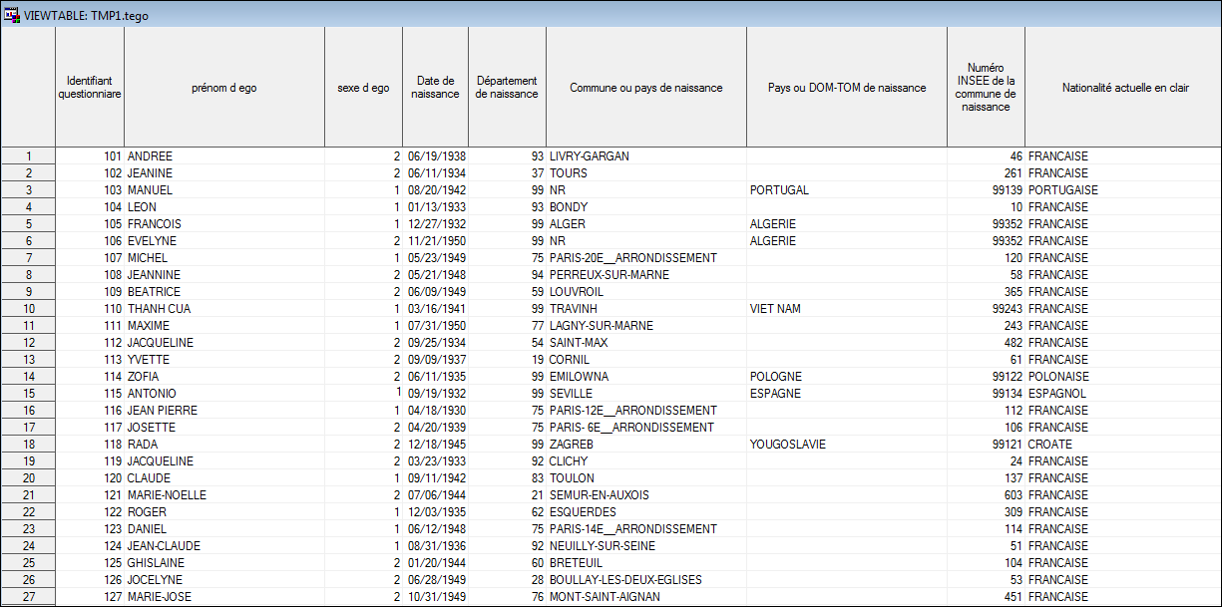
\includegraphics{images/Image1.png}

}

\end{figure}

\begin{figure}

\caption{Biographie et entourage: base biographique logements}

{\centering 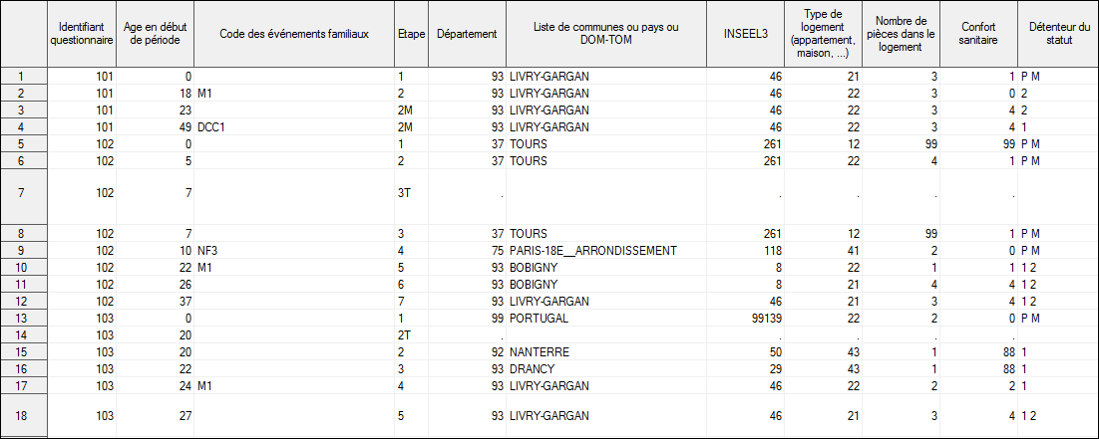
\includegraphics{images/Image2.png}

}

\end{figure}

\hypertarget{enquuxeate-mafe-ined}{%
\subsection{Enquête MAFE (Ined)}\label{enquuxeate-mafe-ined}}

\begin{figure}

\caption{MAFE: base caractéristiques individuelles}

{\centering 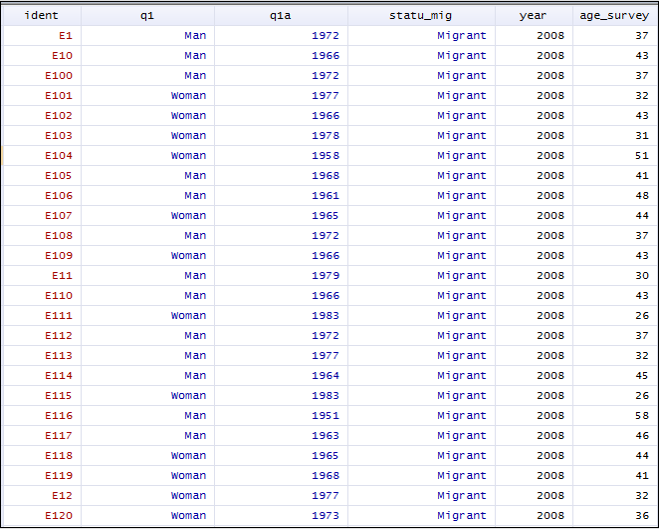
\includegraphics{images/Image3.png}

}

\end{figure}

\begin{figure}

\caption{MAFE: base biographique logement}

{\centering 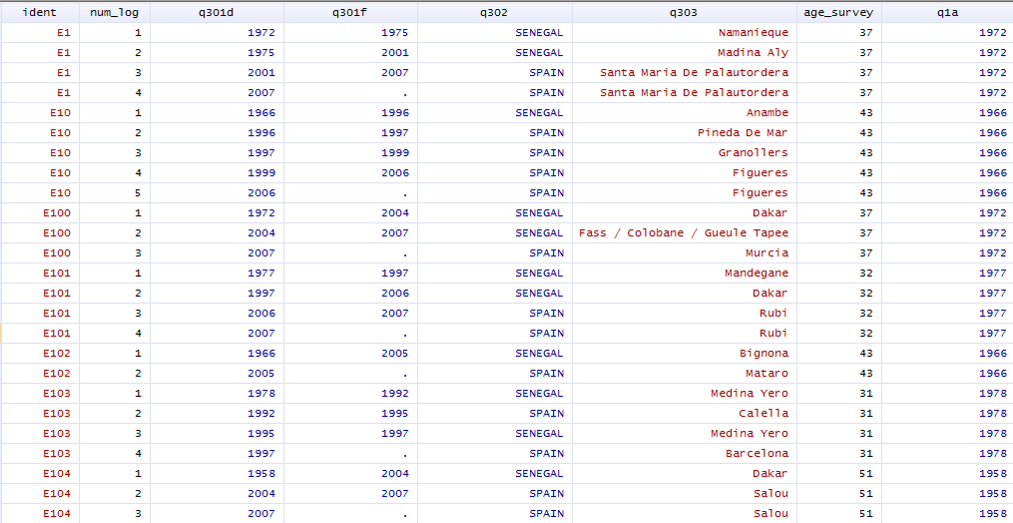
\includegraphics{images/Image4.png}

}

\end{figure}

\hypertarget{la-thuxe9orie}{%
\chapter{\texorpdfstring{\textbf{La
théorie}}{La théorie}}\label{la-thuxe9orie}}

L'analyse des durées peut être vue comme l'étude d'une variable
aléatoire \(T\) qui décrit la durée d'attente jusqu'à l'occurence d'un
évènement.

\begin{itemize}
\tightlist
\item
  La durée \(T=0\) est le début de l'exposition au risque (entrée dans
  le \textbf{Risk set}).
\item
  \(T\) est une mesure non négative de la durée.
\end{itemize}

La principale caractéristique de l'analyse des durées est le traitement
des informations dites \textbf{censurées}, lorsque la \textbf{durée
d'observation est plus courte que la durée d'exposition au risque}.

\hypertarget{temps-et-duruxe9e}{%
\section{\texorpdfstring{\textbf{Temps et
durée}}{Temps et durée}}\label{temps-et-duruxe9e}}

Le temps est une dimension (la quatrième), la durée est sa mesure. La
durée est tout simplement calculée par la différence, pour une échelle
temporelle donnée, entre la fin et le début d'une période d'exposition
ou d'observation.\\
On distingue généralement deux types de mesure de la durée :
\textbf{\emph{continue}} et \textbf{\emph{discrète/groupée}}. Ces deux
notions ne possèdent pas réellement de définition, la différence
s'explique plutôt par la présence ou non de simultanéité dans
l'occurrence des évènements. Le temps étant intrasèquement continu car
deux évènements ne peuvent pas avoir lieu en « même temps ». C'est donc
l'échelle temporelle choisie ou imposée par l'analyse et les données qui
pourra rendre cette mesure continue ou discrète/groupée. Pour un
physicien travaillant sur la théorie de la relativité avec des horloges
atomiques, une minute (voire une seconde) est une mesure très groupée
pour ne pas dire grossière du temps, alors que pour un géologue c'est
une mesure continue. Pour ces deux disciplines, cette échelle de mesure
n'est pas adaptée à leur domaine. Le choix de l'échelle temporelle doit
être pertinent par rapport aux objectifs de l'analyse même si on dispose
des informations très fines (dates de naissance exactes). Etudier la
fécondité avec une métrique journalière n'aurait pas de sens.

Il existe des situations où les durées sont par nature discrète,
lorsqu'un évènement ne peut avoir lieu qu'à un moment précis (date
d'anniversaire des contrats pour l'analyse des résiliation).
Généralement dans les sciences sociales avec un recueil de données de
type rétrospectif, les mesures dites discrètes sont plutôt de nature
groupées. Pour une même année, on considèrera indifféremment des
évènements qui se produiront un premier janvier et un 31 décembre d'une
même année.

\begin{tcolorbox}[enhanced jigsaw, arc=.35mm, bottomrule=.15mm, titlerule=0mm, colbacktitle=quarto-callout-important-color!10!white, left=2mm, opacitybacktitle=0.6, toprule=.15mm, title=\textcolor{quarto-callout-important-color}{\faExclamation}\hspace{0.5em}{Important}, colframe=quarto-callout-important-color-frame, breakable, coltitle=black, opacityback=0, toptitle=1mm, bottomtitle=1mm, rightrule=.15mm, leftrule=.75mm, colback=white]

\begin{itemize}
\tightlist
\item
  \textbf{Durée continue : absence (ou très peu) d'évènements
  simultanés}\\
\item
  \textbf{Durée discrète/groupée : présence d'évènements simultanés (en
  grand nombre)}\\
\end{itemize}

\end{tcolorbox}

\hypertarget{le-risk-set}{%
\section{\texorpdfstring{\textbf{Le Risk
Set}}{Le Risk Set}}\label{le-risk-set}}

\begin{enumerate}
\def\labelenumi{\arabic{enumi}.}
\tightlist
\item
  Il s'agit de la population ``soumise'' ou ``exposée'' au risque
  lorsque \(T=t_i\).
\item
  Cette population varie dans le temps car:

  \begin{itemize}
  \tightlist
  \item
    Certaines personnes ont connu l'évènement, donc ne peuvent plus être
    soumises au risque (ex: décès si on analyse la mortalité).
  \item
    Certaines personnes sortent de l'observation sans avoir (encore)
    observé l'évènement: décès si on analyse un autre type d'évènement,
    perdu.e.s de vue, fin de l'observation dans un recueil rétrospectif.
  \end{itemize}
\end{enumerate}

\hypertarget{la-censure}{%
\section{\texorpdfstring{\textbf{La
Censure}}{La Censure}}\label{la-censure}}

\begin{tcolorbox}[enhanced jigsaw, arc=.35mm, bottomrule=.15mm, titlerule=0mm, colbacktitle=quarto-callout-important-color!10!white, left=2mm, opacitybacktitle=0.6, toprule=.15mm, title=\textcolor{quarto-callout-important-color}{\faExclamation}\hspace{0.5em}{Important}, colframe=quarto-callout-important-color-frame, breakable, coltitle=black, opacityback=0, toptitle=1mm, bottomtitle=1mm, rightrule=.15mm, leftrule=.75mm, colback=white]

\textbf{Une observation est dite censurée lorsque la durée d'observation
est inférieure à la durée d'exposition au risque}

\end{tcolorbox}

\hypertarget{censure-uxe0-droite}{%
\subsection{Censure à droite}\label{censure-uxe0-droite}}

\textbf{Définition}

Certains individus n'auront pas (encore) connu l'évènement à la date de
l'enquête après une certaine durée d'exposition. On a donc besoin d'un
marqueur permettant de déterminer que les individus n'ont pas observé
l'évènement sur la période d'étude.

\textbf{Pourquoi une information est-elle censurée (à droite)?}

\begin{itemize}
\tightlist
\item
  Fin de l'étude, date de l'enquête.
\item
  Perdu de vue, décès si autre évènement étudié.
\end{itemize}

En pratique (important)

\begin{itemize}
\tightlist
\item
  \textbf{Ne pas exclure ces observations}, sinon on surestime la
  survenue de l'évènement.
\item
  \textbf{Ne pas les considérer a-priori comme sorties de l'exposition
  sans avoir connu l'évènement}. Elles peuvent connaître l'évènement
  après la date de l'enquête ou en étant perdues de vue. Sinon on
  sous-estime la durée moyenne de survenue de l'évènement.
\end{itemize}

\textbf{Exemple}\\
On effectue une enquête auprès de femmes : On souhaite mesurer l'âge à
la première naissance. Au moment de l'enquête, une femme est âgée de 29
ans n'a pas (encore) d'enfant.\\
Cette information sera dite «censurée».\\
Elle est clairement encore soumise au risque après la date de l'enquête.
Au niveau de l'analyse, elle sera soumise au risque à partir de ses
premières règles jusqu'au moment de l'enquête.

\textbf{Hypothèse fondamentale}\\
Les observations censurées ont vis à vis du phénomène observé le même
comportement que les observations non censurées. On dit que la
\textbf{censure est non informative}. Elle ne dépend pas de l'évènement
analysé. Normalement le problème ne se pose pas dans les recueil
retrospectif.

\emph{Problème posé par la censure informative}\\
Par exemple en analysant des décès avec un recueil prospectif, si un
individu est perdu de vue en raison d'une dégradation de son état de
santé, l'indépendance entre la cause de la censure et le décès ne peut
plus être assurée.\\
A l'Ined l'exploitation du registre des personnes atteintes de
mucoviscidose (G.Bellis) donne une autre illustration de ce phénomène.
Chaque année un nombre significatif de personnes sortent du registre
(pas de résultats aux examens annuels). Si certain.e.s perdu.e.s de vue
s'expliquent par des déménagements, émigration ou par un simple problème
d'enregistrement des informations, on note qu'ils/elles sont
nombreu.se.s à présenter une forme « légère » de la maladie.
L'information pouvant être donnée ici par la mutation du gène. Comme il
n'est pas recommandé de supprimer ou de traiter ces observations comme
des censures à droite non informatives, on peut les appréhender comme un
risque concurrent au décès ou à tout autre évènement analysé à partir de
ce registre (voir section dédiée).

Les graphiques suivant représentent, en temps calendaire et après sa
transformation en durée, la logique des censures à droite. Le recueil
des informations est ici de nature prospectives.

\begin{itemize}
\tightlist
\item
  Trait plein : durée observée
\item
  Pointillés : durée censurée
\item
  Bulle : moment de l'évènement
\end{itemize}

\begin{figure}

\caption{Schéma évènement/censure en temps calendaire}

{\centering 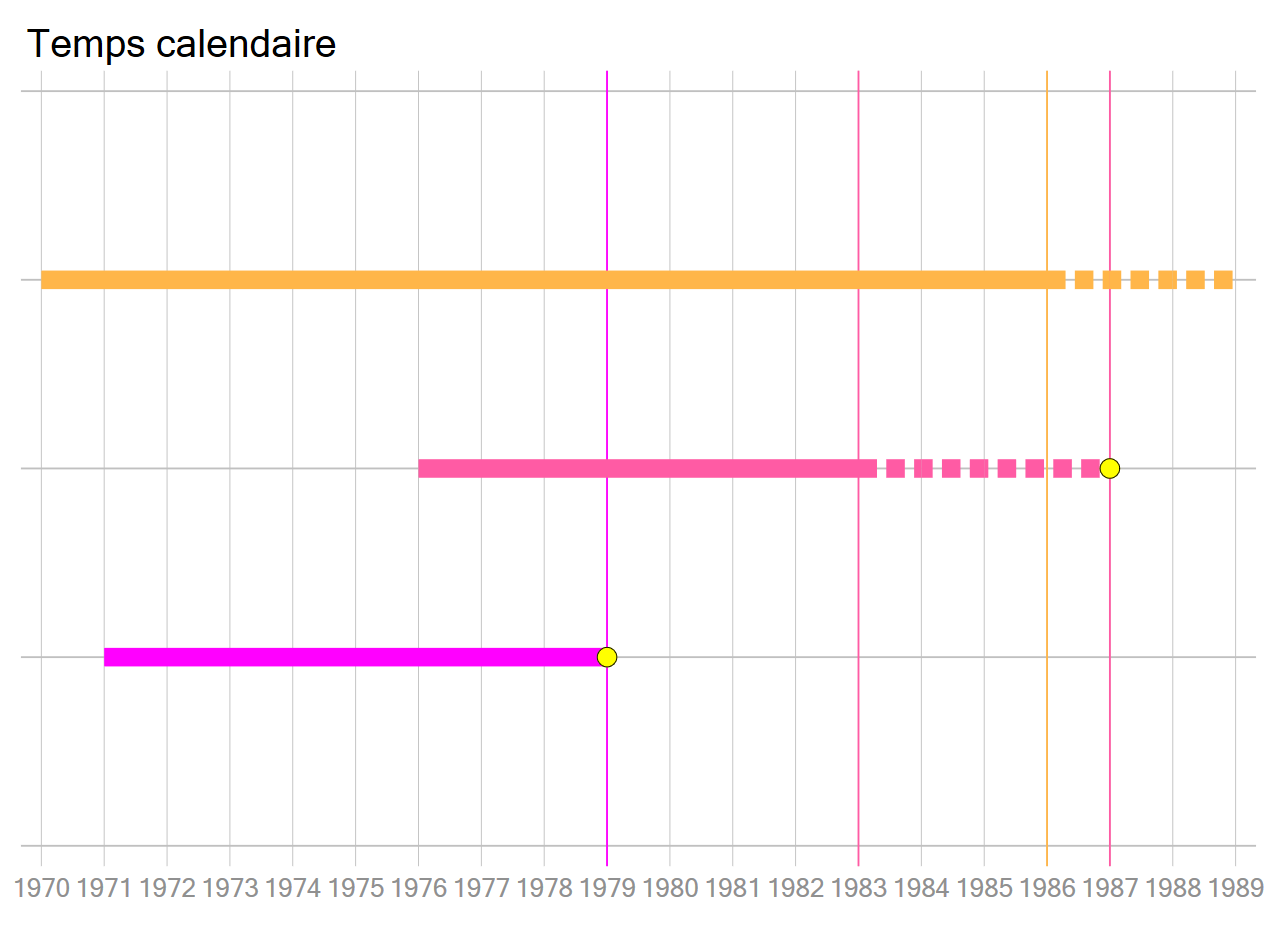
\includegraphics[width=0.7\textwidth,height=\textheight]{images/cens1.png}

}

\end{figure}

\begin{figure}

\caption{Schéma évènement/censure sous forme de durée}

{\centering 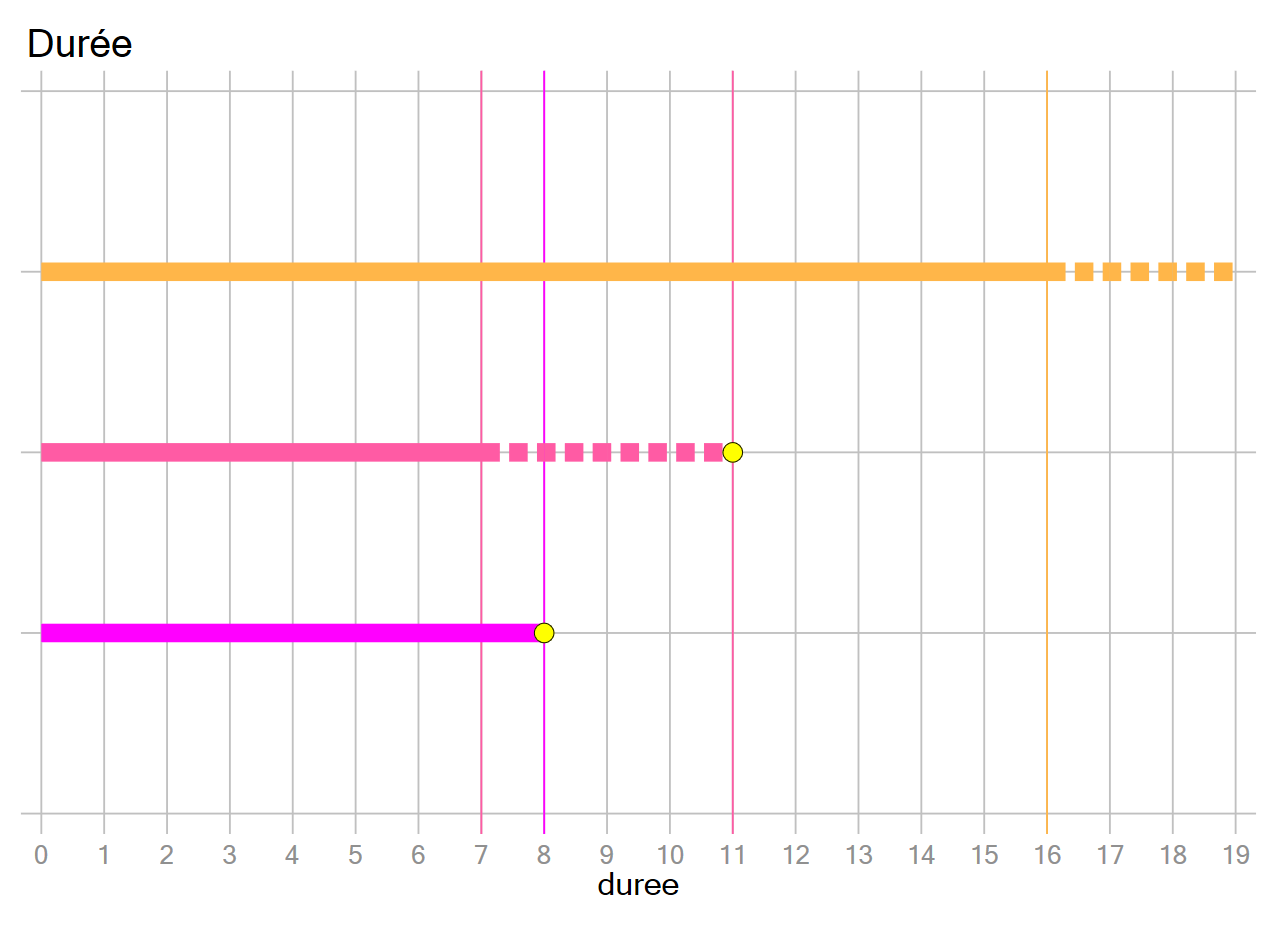
\includegraphics[width=0.7\textwidth,height=\textheight]{images/cens2.png}

}

\end{figure}

\hypertarget{censure-uxe0-gauche-troncature-et-censure-par-intervalle}{%
\subsection{Censure à gauche, troncature et censure par
intervalle}\label{censure-uxe0-gauche-troncature-et-censure-par-intervalle}}

\textbf{Censure à gauche}\\
L'évènement s'est produit avant le début période d'observation. Typique
des données prospectives, de type registre, avec des âges d'inclusion
différenciés.

\textbf{Censure par intervalle} Un évènement peut se produire entre 2
temps d'observations sans qu'on puisse les observer (ex: en criminologie
récidive d'un delit entre deux arrestations). Un phénomène de censure à
droite avec perdu.e de vue peut se transformer en censure par intervalle
lorsque la personne réapparait et est de nouveau incluse dans les
données.

\textbf{Troncature}\\
Par l'exemple, on analyse la survie d'une population. Seule la survie
des individus vivants à l'inclusion peut être analysée (\emph{troncature
à gauche}). On peut également trouver un phénomène de troncature
lorsqu'on mesure la durée à partir ou jusqu'à un certain seuil niveau.

Ces situations sont généralement plutôt bien contrôlées dans les
recueils rétrospectifs. Elles sont assez courantes lorsque le recueil
est de type prospectif.

\textbf{Durée d'observation supérieure à la durée d'exposition}\\
A l'inverse des individus peuvent sortir de l'exposition avant la fin de
la période d'observation, et il convient donc de corriger la durée de
cette sortie.\\
Un exemple simple : si au moment de l'enquête une femme sans enfant a 70
ans, cela n'a pas de sens de continuer de l'exposer au risque au-delà
d'un certain âge. Si on ne dispose pas d'information sur l'âge à la
ménopause on peut tronquer la durée un peu au-delà de l'âge le plus
élevé à la première naissance observée dans les données.

\hypertarget{les-grandeurs}{%
\section{\texorpdfstring{\textbf{Les
grandeurs}}{Les grandeurs}}\label{les-grandeurs}}

\hypertarget{les-grandeurs-utilisuxe9es}{%
\subsection{\texorpdfstring{\textbf{Les grandeurs
utilisées}}{Les grandeurs utilisées}}\label{les-grandeurs-utilisuxe9es}}

\begin{itemize}
\item
  La fonction de survie: \textbf{\(S(t)\)}
\item
  La fonction de répartition: \textbf{\(F(t)\)}
\item
  La fonction de densité: \textbf{\(f(t)\)}
\item
  Le risque \emph{instantané}: \textbf{\(h(t)\)}
\item
  Le risque \emph{instantané} cumulé: \textbf{\(H(t)\)}
\end{itemize}

\textbf{Remarques}:

\begin{itemize}
\tightlist
\item
  Toutes ces grandeurs sont mathématiquement liées les unes par rapport
  aux autres. En connaître une permet d'obtenir les autres.\\
\item
  Au niveau formel on se placera ici du point de vue où la durée mesurée
  est strictement continue. Cela se traduit, entre autre, par l'absence
  d'évènements dits ``simultanés''.
\item
  Les expressions qui vont suivre ne sont pas des estimateurs, mais des
  grandeurs dont on précisera les propriétés. Les techniques
  d'estimations devront respecter ces propriétés .
\end{itemize}

\hypertarget{la-fonction-de-survie-st}{%
\subsection{\texorpdfstring{La fonction de Survie
\(S(t)\)}{La fonction de Survie S(t)}}\label{la-fonction-de-survie-st}}

Dans ce type d'analyse, il est courant d'analyser la courbe dite de
survie. Hors contexte de mortalité on peut préférer la notion de
\textbf{courbe de de séjour} (Courgeau, Lelièvre).

\textbf{La fonction de survie donne la proportion de la population qui
n'a pas encore connue l'évènement après une certaine durée \(t\)}. Elle
y a donc ``survécu''.

Formellement, la fonction de survie est la probabilité de survivre
au-delà de \(t\), soit:\\

\[S(t) = P(T>t)\]

Propriétés:

\begin{itemize}
\tightlist
\item
  \(S(0)=1\)
\item
  \(\lim\limits_{t\to{\propto}}S(t)=0\)
\end{itemize}

La fonction de survie est donc strictement non croissante.

\hypertarget{la-fonction-de-ruxe9partition-ft}{%
\subsection{\texorpdfstring{La fonction de répartition
\(F(t)\)}{La fonction de répartition F(t)}}\label{la-fonction-de-ruxe9partition-ft}}

C'est la probabilité de connaitre l'évènement jusqu'en \(t\), soit:\\

\[F(t)=P(T\leq{t})\]

Soit: \(F(t) = 1 - S(t)\)

La fonction de survie et la fonction de répartition sont donc deux
grandeurs strictement complémentaires et décrivent la même information.

Propriétés:

\begin{itemize}
\tightlist
\item
  \(F(0)=0\)
\item
  \(\lim\limits_{t\to{\propto}}F(t)=1\)
\end{itemize}

\hypertarget{la-fonction-de-densituxe9-ft}{%
\subsection{\texorpdfstring{La fonction de densité
\(f(t)\)}{La fonction de densité f(t)}}\label{la-fonction-de-densituxe9-ft}}

\begin{itemize}
\tightlist
\item
  Pour une valeur de \(t\) donnée, la fonction de densité de l'évènement
  donne la distribution des moments où les évènement ont eu lieu. Elle
  est donnée dans un premier temps par la probabilité de connaitre
  l'évènement dans un petit intervalle de temps \(dt\). Si \(dt\) est
  proche de 0 (temps continu) alors cette probabilité tend également
  vers 0. On norme donc cette probabilité par \(dt\). Rappel: on est
  toujours ici dans la théorie.\\
\item
  En temps continu, la fonction de densité est donnée par la dérivée de
  la fonction de répartition: \(f(t)=F'(t)=-S'(t)\).
\end{itemize}

Formellement la fonction de densité \(f(t)\) s'écrit:

\[f(t)=\lim\limits_{dt\to{0}}  \frac{P(t\leq{T}< t + dt)}{dt}\]

\hypertarget{le-risque-instantanuxe9-ht}{%
\section{\texorpdfstring{Le risque instantané
\(h(t)\)}{Le risque instantané h(t)}}\label{le-risque-instantanuxe9-ht}}

Concept fondamental de l'analyse des durées:

\[h(t)=\lim\limits_{dt\to{0}} \frac{P(t\leq{T}< t + dt | T\geq{t})}{dt}\]

\begin{itemize}
\tightlist
\item
  \(P(t\leq{T}< t + dt | T\geq{t})\) donne la probabilité de survenue de
  l'évènement sur l'intervalle \([t,t+dt[\) \emph{conditionnellement à
  la survie au temps \(t\)}.\\
\item
  En divisant par \(dt\), La quantité obtenue donne alors un nombre
  moyen d'évènements que connaîtrait un individu durant un très court
  intervalle de temps.
\item
  A priori cette quantité n'est pas une probabilité. C'est la nature de
  l'évènement, en particulier sa non récurrence, et la métrique
  temporelle choisie ou disponible qui peut la rendre assimilable à une
  probabilité. Tout comme la densité, on est plutôt dans la définition
  d'un \emph{taux} (d'où l'expression \textbf{\emph{hazard rate}} en
  anglais).
\end{itemize}

On peut également écrire:
\(h(t)=\frac{f(t)}{S(t)}=\frac{F'(t)}{S(t)}=-\frac{S'(t)}{S(t)}\)

On remarque que la fonction de risque n'est pas une probabilité car
\(\frac{f(t)}{S(t)}\) ne peut pas contraindre la valeur obtenue à ne pas
être supérieure à 1.

\hypertarget{le-risque-cumuluxe9-ht}{%
\subsection{\texorpdfstring{Le risque cumulé
\(H(t)\)}{Le risque cumulé H(t)}}\label{le-risque-cumuluxe9-ht}}

Le risque cumulé est égal à :

\[H(t)=\int_{0}^{t} h(u)du = -log(S(t))\]

On peut alors réécrire toutes les autres quantités à partir de celle-ci:

\begin{itemize}
\tightlist
\item
  \(S(t)=e^{-H(t)}\)\\
\item
  \(F(t)=1-e^{-H(t)}\)\\
\item
  \(f(t)=h(t)\times{e^{-H(t)}}\)
\end{itemize}

\emph{Exemple avec la loi exponentielle (risque constant)}

Si on pose que le risque est strictement constant au cours du temps:
\(h(t)=a\). Cette forme du risque suit une \textbf{loi exponentielle}.
Cette situation est, par exemple, typique des processus dits sans
mémoire comme la durée de vie des ampoules:

\begin{itemize}
\tightlist
\item
  \(h(t)=a\)\\
\item
  \(H(t)=a\times{t}\)\\
\item
  \(S(t)=e^{-a\times{t}}\)\\
\item
  \(F(t)=1-e^{-a\times{t}}\)\\
\item
  \(f(t)=a\times{e^{-a\times{t}}}\)
\end{itemize}

\begin{figure}

\caption{Grandeurs de la loi exponentielle avec h(t)=0.04}

{\centering 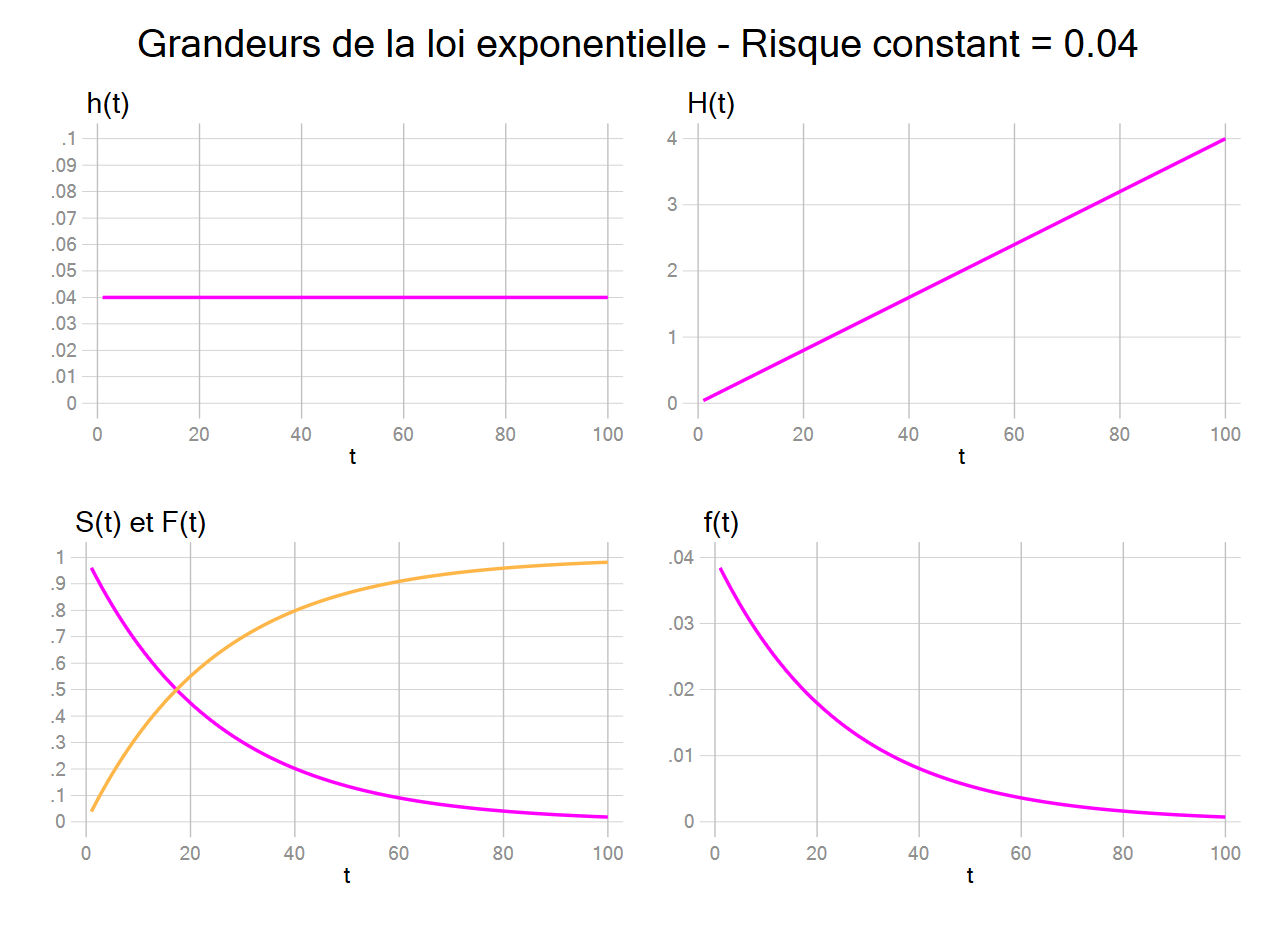
\includegraphics[width=0.7\textwidth,height=\textheight]{images/Image5.png}

}

\end{figure}

\textbf{Application: risque et échelles temporelles}:

Attention on sort ici très clairement de la durée continue, il s'agit
seulement de manipuler les concepts et de voir la dépendance de la
mesure du risque à l'échelle temporelle choisie ou disponible.

\begin{enumerate}
\def\labelenumi{\arabic{enumi}.}
\item
  Durant les mois d'hiver, entre le 1er janvier et le 1er avril {[}3
  mois{]}, la probabilité d'attraper un rhume chaque mois est de 48\%
  (il s'agit bien d'un risque). Quelle est le risque d'attraper le rhume
  durant la saison froide?\\
  \(\frac{0.48}{1/3}=1.44\). On peut donc s'attendre a attraper 1.44
  rhume durant la période d'hiver.
\item
  On passe une année en vacances dans une région où la probabilité de
  décéder chaque mois est évaluée à 33\%. Quelle est le risque de
  décéder pendant cette année sabbatique? \(\frac{0.33}{1/12}=3.96\)
\end{enumerate}

Le risque peut donc être supérieur à 1. C'est donc plutôt un taux tel
qu'il est défini généralement. En soit cela ne pose pas de problème
comme il s'agit d'un nombre moyen d'évènements espérés (exemple:
\emph{taux} de fécondité), mais pour des évènements qui ne peuvent pas
se répéter, évènements dits \emph{absorbants}, l'interprétation n'est
pas très intuitive.

Le risque étant constant, on peut prendre son inverse qui mesure la
durée moyenne (espérée) jusqu'à l'occurence de l'évènement.\\
On retrouve donc un concept classique en analyse démographique comme
l'espérance de vie (survie): la question n'est pas de savoir si on va
mourir ou non, ce risque indépendamment de la durée étant par définition
égal à 1, mais jusqu'à quand on peut espérer survivre.

\begin{itemize}
\tightlist
\item
  Pour le rhume, la durée moyenne est de \((1.44^{-1}=0.69\) du
  trimestre hivernal, soit approximativement le début du mois de mars.
\item
  Pour l'année sabbatique, la durée moyenne de survie est de
  \(3.96^{-1}=0.25\) d'une année soit 3 mois après l'arrivée dans la
  région.
\end{itemize}

\textbf{Exercice}

\begin{itemize}
\tightlist
\item
  On a une population de 100 cochons d'Inde.
\item
  On analyse leur mortalité (naturelle).\\
\item
  Ici l'analyse est en temps discret.
\item
  La durée représente le nombre d'année de vie.
\item
  Il n'y a pas de censure à droite.
\end{itemize}

\begin{longtable}[]{@{}ll@{}}
\toprule\noalign{}
Durée & Nombre de décès \\
\midrule\noalign{}
\endhead
\bottomrule\noalign{}
\endlastfoot
1 & 1 \\
2 & 1 \\
3 & 3 \\
4 & 9 \\
5 & 30 \\
6 & 40 \\
7 & 10 \\
8 & 3 \\
9 & 2 \\
10 & 1 \\
\end{longtable}

\textbf{N=100}

A quel âge le risque de mourir des cochons d'Inde est-il le plus élevé?
Quelle est la valeur de ce risque?

\hypertarget{remarques-compluxe9mentaires}{%
\section{\texorpdfstring{\textbf{Remarques
complémentaires}}{Remarques complémentaires}}\label{remarques-compluxe9mentaires}}

\hypertarget{formes-typiques-de-la-fonction-de-survie}{%
\subsection{Formes typiques de la fonction de
survie}\label{formes-typiques-de-la-fonction-de-survie}}

Une des propriétés de la fonction de survie ou de séjour est qu'elles
tendent vers 0. A la lecture du graphique suivant, cela peut
correspondre à la forme de la courbe S2, bien que le \% de survivant
tend à baisser de moins en moins à mesure que la durée augmente. Deux
cas limites doivent être considéré.

\begin{figure}

\caption{Fonction de survie: 3 situtation typiques}

{\centering 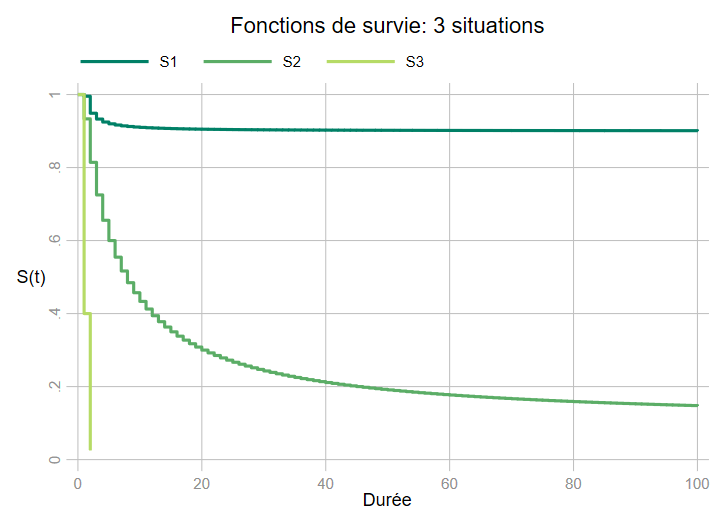
\includegraphics[width=0.9\textwidth,height=\textheight]{images/Image5b.png}

}

\end{figure}

\begin{itemize}
\item
  \textbf{S1}: très peu d'évènements et la fonction de séjour suit une
  asymptote nettement supérieur à 0 (
  \(\lim\limits_{t\to{\propto}}S(t)=a\) avec \(a>0\)). La question est
  plus délicate car on interroge l'exposition au risque d'une partie de
  l'échantillon ou, dit autrement on peut penser qu'une fraction est
  immunisé au risque. Cette problématique est rapidement posée en fin de
  formation.
\item
  \textbf{S2}: la situation attendue
\item
  \textbf{S3}: La survie tombe à 0 très/trop rapidement: il n'y a donc
  pas ou presque pas de durée (par exemple presque tout l'échantillon
  observe l'évènement la première année de l'exposition). Les méthodes
  en temps continue ne sont a priori pas adaptées à ce genre de
  situation. Si on dispose d'une information plus fine pour dater les
  évènements, la fonction de séjour pourra reprendre une forme plus
  ``standard''. Dans le graphique, \(S(t=1)=0.4\) , \(S(t=2)=0.025\),
  mais si on dispose par exemple de 10 points d'observations
  supplémentaires dans chaque durée groupée:
\end{itemize}

\begin{figure}

\caption{Fonction de survie et modification de la métrique temporelle}

{\centering 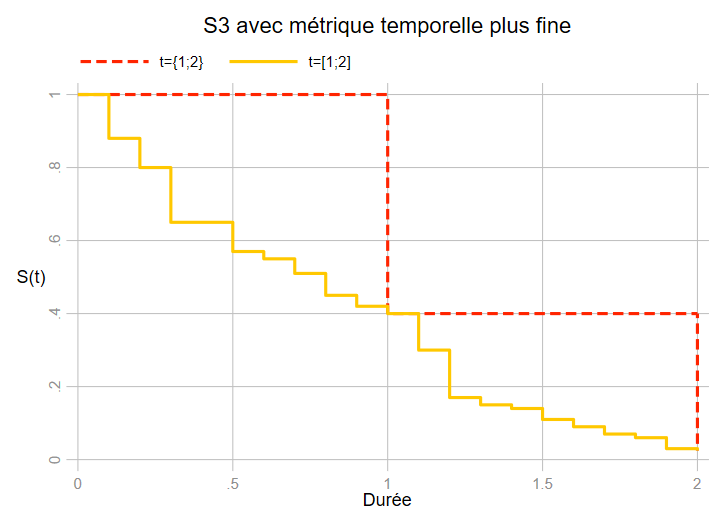
\includegraphics[width=0.9\textwidth,height=\textheight]{images/Image5c.png}

}

\end{figure}

\hypertarget{absence-de-censures-uxe0-droites}{%
\subsection{Absence de censures à
droites}\label{absence-de-censures-uxe0-droites}}

Les méthodes qui vont être présentées plus tard \textbf{\emph{gèrent}}
la présence de censures à droite. S'il n'y en a pas, elle restent
néanmoins parfaitement valables. L'absence de censure facilite certaines
analyses, par exemple celles des fonctions de séjour où le calcul direct
des durées moyennes est rendu possible.

\hypertarget{utilisation-des-ponduxe9rations-dans-un-schema-retrospectif-avec-des-biographies-longues}{%
\subsection{Utilisation des pondérations dans un schema retrospectif
avec des biographies
longues}\label{utilisation-des-ponduxe9rations-dans-un-schema-retrospectif-avec-des-biographies-longues}}

Une question assez récurrente concerne l'utilisation des poids de
sondage dans les analyses de durées avec longueurs biographiques souvent
assez longues. Leur utilisation ne me semble pas recommandée voire à
exclure sauf exceptions. En effet les pondérations sont générées au
moment de l'enquête, alors que les évènements étudiés peuvent remonter
dans un passé plus ou moins lointain pour une partie de la population
analysée. Si on regarde de plus près, la création de poids longitudinaux
ne résoudrait pas grand chose , les pondérations devant être recalculées
à chaque moment d'observation ou à chaque moment où des évènements se
produisent. Par ailleurs on mélangerait régulièrement à un instant donné
des personnes issues de générations différentes ce qui rend impossible
tout calage sur des caractéristiques d'un population. Supposons une
personne âgée de 25 ans et un personne âgée de 70 ans au moment de
l'enquête en 2022, avec un début d'observation à l'âge de 18 ans . A 20
ans (\(t=2\)), pour la première personne les caractéristiques de la
population sont celles de 2017, pour celle de 70 ans celles de 1972. On
fait comment??????

\part{Méthodes non paramétrique}

\hypertarget{estimations-des-fonctions-de-survie}{%
\chapter{\texorpdfstring{\textbf{Estimations des fonctions de
survie}}{Estimations des fonctions de survie}}\label{estimations-des-fonctions-de-survie}}

Les méthodes non paramétriques portent généralement sur l'analyse des
fonctions de survie (\(S(t\))) ou sur celles des fonctions de
répartitions (\(F(t)\)), plus rarement sur les mesures d'incidence
données par le risque cumulé. Deux méthodes d'estimations sont proposées
: la méthode dite actuarielle et la méthode dite de Kaplan \& Meier. Ces
deux approches sont adaptées à des mesures différentes de la durée :
plutôt discrète/groupée pour la technique actuarielle et plutôt continue
pour Kaplan-Meier (KM). Cela induit un traitement différent de la
censure dans l'estimation. La seconde est de très très loin la plus
utilisée, en partie en raison des tests de comparaison, plus ou moins
pertinents, qu'elle permet de réaliser.

\begin{tcolorbox}[enhanced jigsaw, arc=.35mm, bottomrule=.15mm, titlerule=0mm, colbacktitle=quarto-callout-important-color!10!white, left=2mm, opacitybacktitle=0.6, toprule=.15mm, title=\textcolor{quarto-callout-important-color}{\faExclamation}\hspace{0.5em}{Important}, colframe=quarto-callout-important-color-frame, breakable, coltitle=black, opacityback=0, toptitle=1mm, bottomtitle=1mm, rightrule=.15mm, leftrule=.75mm, colback=white]

\begin{itemize}
\tightlist
\item
  J'insiste sur la nécessité de passer par cette étape avant de se
  lancer \emph{corps perdu} dans des modèles, comme ceux à durée
  discrète.

  \begin{itemize}
  \tightlist
  \item
    Les applications ont des gardes fous permettant d'alerter sur des
    durées d'exposition incorrecte, en particulier lorsqu'on travaille
    sur des données prospectives.
  \item
    Egalement très utile, la comparaison graphique de courbes de séjour
    permet de repérer rapidement des violations fortes de l'hypothèse de
    proportionalité des risques, ou des situations de quasi
    \emph{immunité}.
  \end{itemize}
\item
  Concernant les tests non paramétriques, ceux utilsant la technique du
  \emph{logrank}, présente à mon sens tellement de défauts qu'ils
  devraient être abandonné. Malheureusement encore très peu diffusée
  dans les sciences sociales, la comparaison des RMST (\emph{Restricted
  Mean of Survival Time}) me semble une solution largement supérieure,
  tant au niveau statistique qu'au niveau interprétatif.
\end{itemize}

\end{tcolorbox}

\hypertarget{les-fonctions-de-surviesuxe9jour}{%
\section{\texorpdfstring{\textbf{Les fonctions de
survie/séjour}}{Les fonctions de survie/séjour}}\label{les-fonctions-de-surviesuxe9jour}}

\hypertarget{les-variables-danalyse}{%
\subsection{Les variables d'analyse}\label{les-variables-danalyse}}

On a un échantillon aléatoire de \(n\) individus avec:

\begin{itemize}
\tightlist
\item
  Des indicateurs de fin d'épisode \(e_1,e_2,....,e_k\) avec \(e_i=0\)
  si censure à droite et \(e_i=1\) si évènement observé pendant la
  période d'observation.
\item
  Des durées d'exposition au risque \(t_1,t_2,....,t_k\) jusqu'à
  l'évènement ou la censure.
\item
  En théorie, il ne peut pas y avoir d'évènement en \(t=0\).
\end{itemize}

\hypertarget{calcul-de-la-fonction-de-survie}{%
\subsection{Calcul de la fonction de
survie}\label{calcul-de-la-fonction-de-survie}}

Rappel: La fonction de survie donne la probabilité que l'évènement
survienne après \(t_i\), soit \(S(t_i)=P(T>t_i)\). Pour survivre en
\(t_i\), il faut donc avoir survécu en \(t_{i-1}\), \(t_{i-2}\),
\ldots., \(t_{1}\).\\
La fonction de survie renvoie donc des probabilités conditionnelles: on
survit en \(t_i\) conditionnellement au fait d'y avoir survécu avant. Il
s'agit donc d'un produit de probabilités.

Soit \(d_i=\sum e_i\) le nombre d'évènements observé en \(t_i\) et
\(r_i\) la population encore soumise au risque en \(i\). On peut mesurer
l'intensité de l'évènement en \(t_i\) en calculant le quotient
\(q(t_i)=\frac{d_i}{r_i}\).

Si le temps est strictement continu on devrait toujours avoir
\(q(t_i)=\frac{1}{r_i}\).

\(S(t_i) = (1 - \frac{d_i}{r_i})\times{S(t_{i-1})} = S(t_i) = (1 - q(t_i))\times{S(t_{i-1})}\).
En remplaçant \(S(t_{i-1})\) par sa valeur:
\(S(t_i) = (1 - \frac{d_i}{r_i})\times(1 - \frac{d_{i-1}}{r_{i-1}})\times{S(t_{i-2})}\).

Au final, en remplaçant toutes les expressions de la survie jusqu'en
\(t_0\) (\(S(0)=1\)):

\[S(t_i)=\displaystyle \prod_{t_i\leq{k}} (1-q(t_i))\]

\begin{tcolorbox}[enhanced jigsaw, arc=.35mm, bottomrule=.15mm, titlerule=0mm, colbacktitle=quarto-callout-note-color!10!white, left=2mm, opacitybacktitle=0.6, toprule=.15mm, title=\textcolor{quarto-callout-note-color}{\faInfo}\hspace{0.5em}{Application pour la suite du support}, colframe=quarto-callout-note-color-frame, breakable, coltitle=black, opacityback=0, toptitle=1mm, bottomtitle=1mm, rightrule=.15mm, leftrule=.75mm, colback=white]

\begin{itemize}
\item
  On va analyser le risque de décéder (la survie) de personnes souffrant
  d'une insuffisance cardiaque. Le début de l'exposition est leur
  inscription dans un registre d'attente pour une greffe du coeur.
\item
  Les covariables sont dans un premier temps toutes fixes: l'année
  (\emph{year}) et l'âge (\emph{age}) à l'entrée dans le registre, et le
  fait d'avoir été opéré pour un pontage aorto-coronarien avant
  l'inscription (\emph{surgery}).
\item
  Le début de l'exposition au risque est l'entrée dans le registre, la
  durée est mesurée en jour (\emph{stime}). La variable
  évènement/censure est le décès (\emph{died}). Les durées de la
  variable \emph{stime} ont été regroupée par période de 30 jours pour
  réaliser des analyses à durée discrete. Cette nouvelle variable de
  durée a été appelé \emph{mois}.
\item
  L'introduction d'une dimension dynamique, la greffe, est donnée par
  les informations contenues dans les variables \emph{transplant} et
  \emph{wait}.
\item
  La variable \emph{compet} est une information simulée pour réaliser
  des analyses en risques concurrents.
\item
  Les bases en format .csv, .sas7bdat et .dta sont disponibles dans ce
  dépôt
  {[}\href{https://github.com/mthevenin/analyse_duree/tree/main/bases}{lien}{]}
\end{itemize}

Extrait de la base:

\begin{longtable}[]{@{}
  >{\raggedright\arraybackslash}p{(\columnwidth - 18\tabcolsep) * \real{0.0714}}
  >{\raggedright\arraybackslash}p{(\columnwidth - 18\tabcolsep) * \real{0.0857}}
  >{\raggedright\arraybackslash}p{(\columnwidth - 18\tabcolsep) * \real{0.0714}}
  >{\raggedright\arraybackslash}p{(\columnwidth - 18\tabcolsep) * \real{0.0857}}
  >{\raggedright\arraybackslash}p{(\columnwidth - 18\tabcolsep) * \real{0.1000}}
  >{\raggedright\arraybackslash}p{(\columnwidth - 18\tabcolsep) * \real{0.1286}}
  >{\raggedright\arraybackslash}p{(\columnwidth - 18\tabcolsep) * \real{0.1714}}
  >{\raggedright\arraybackslash}p{(\columnwidth - 18\tabcolsep) * \real{0.0857}}
  >{\raggedright\arraybackslash}p{(\columnwidth - 18\tabcolsep) * \real{0.0857}}
  >{\raggedright\arraybackslash}p{(\columnwidth - 18\tabcolsep) * \real{0.1143}}@{}}
\toprule\noalign{}
\begin{minipage}[b]{\linewidth}\raggedright
id
\end{minipage} & \begin{minipage}[b]{\linewidth}\raggedright
year
\end{minipage} & \begin{minipage}[b]{\linewidth}\raggedright
age
\end{minipage} & \begin{minipage}[b]{\linewidth}\raggedright
died
\end{minipage} & \begin{minipage}[b]{\linewidth}\raggedright
stime
\end{minipage} & \begin{minipage}[b]{\linewidth}\raggedright
surgery
\end{minipage} & \begin{minipage}[b]{\linewidth}\raggedright
transplant
\end{minipage} & \begin{minipage}[b]{\linewidth}\raggedright
wait
\end{minipage} & \begin{minipage}[b]{\linewidth}\raggedright
mois
\end{minipage} & \begin{minipage}[b]{\linewidth}\raggedright
compet
\end{minipage} \\
\midrule\noalign{}
\endhead
\bottomrule\noalign{}
\endlastfoot
15 & 68 & 53 & 1 & 1 & 0 & 0 & 0 & 1 & 1 \\
43 & 70 & 43 & 1 & 2 & 0 & 0 & 0 & 1 & 1 \\
61 & 71 & 52 & 1 & 2 & 0 & 0 & 0 & 1 & 1 \\
75 & 72 & 52 & 1 & 2 & 0 & 0 & 0 & 1 & 1 \\
102 & 74 & 40 & 0 & 11 & 0 & 0 & 0 & 1 & 0 \\
74 & 72 & 29 & 1 & 17 & 0 & 1 & 5 & 1 & 2 \\
\end{longtable}

\end{tcolorbox}

\hypertarget{la-muxe9thode-actuarielle}{%
\section{\texorpdfstring{\textbf{La méthode
actuarielle}}{La méthode actuarielle}}\label{la-muxe9thode-actuarielle}}

\begin{itemize}
\tightlist
\item
  Estimation sur des intervalles définies par l'utilisateur.
\item
  Méthode dite «continue», estimation en milieu d'intevalle.
\item
  Méthode apropriée lorsque la durée est mesurée de manière
  discrète/groupée.
\item
  Méthode, hélas, quasiment abandonnée dans les sciences sociales où les
  durées sont plus rarement mesurées de manière exacte. L'absence de
  test de comparaison des fonctions de survie n'y est pas étranger, tout
  comme le lien de la méthode suivante (Kaplan-Meier) avec le modèle de
  Cox.
\item
  Contrairement à la méthode de Cox, la méthode actuarielle permet de
  calculer les quantiles de la durée.
\end{itemize}

\hypertarget{estimation}{%
\subsection{Estimation}\label{estimation}}

\textbf{Echelle temporelle}

La durée est divisée en \(J\) intervalles, en choisissant \(J\) points:
\(t_0<t_1<...<t_J\) avec \(t_{J+1}=\infty\).

\textbf{Calcul du Risk set}

\begin{itemize}
\tightlist
\item
  A \(t_{min}=0\), \(n_0=n\) individus soumis au risque: \(r_0=n_0\).
\item
  Le nombre d'exposé.e.s au risque sur un intervalle est calculé en
  soustrayant la moitié des cas censurés sur la longueur de
  l'intervalle: \(r_i=n_i- 0.5\times{c_i}\), avec \(n_i\) le nombre de
  personnes soumises au risque au début de l'intervalle et \(c_i\) le
  nombre d'observations censurées sur la longueur de l'intervalle. On
  suppose donc que les observations censurées \(c_i\) sont sorties de
  l'observation uniformément sur l'intervalle. Les cas censurés le sont
  en moyenne au millieu de l'intervalle.
\end{itemize}

\textbf{Calcul de} \(S(t_i)\)\\
On applique la méthode de la section précédente avec:

\[q(t_i)=\frac{d_i}{n_i - 0.5\times c_i}\]

\textbf{Calcul de la durée médiane (ou autre quantiles)}

\emph{Rappel}: en raison de la présence de censures à droite, le dernier
intervalle étant ouvert jusqu'à la dernière sortie d'observation, il
n'est pas conseillé de calculer des durées moyennes. On préfère utiliser
la médiane ou tout autre quantile lorsqu'ils sont calculables.

\textbf{Définition}: il s'agit de la durée telle que \(S(t_i)=0.5\).

\emph{Calcul}: Comme on applique une méthode continue et monotone à
l'intérieur d'intervalles, on ne peut pas calculer directement un point
de coupure qui correspond à 50\% de survivants. On doit donc trouver ce
point par interpolation linéaire dans l'intervalle \([t_i;t_{i+1}[\)
avec \(S(t_{i+1})\leq0.5\) et \(S(t_{i})>0.5\).

\textbf{R-Stata-Sas-Python}

\subsection{R}

Les fonctions de survie avec la méthode dite actuarielle sont estimables
avec le package \textbf{\texttt{discSurv}}. Avec le temps, il s'est
étoffé, on peut maintenant paramatrer des intervalles (programmation
pénible), mais les quantiles de la durée ne sont toujours pas
estimables, ce qui est bien dommage.

\subsection{Stata}

Commande \texttt{ltable}, avec en option la paramétrisation des
intervalles de durées. Voir la commande externe \texttt{qlt} (MT) qui
calcule les durées médianes (+ autres quartiles) et qui recalcule la
fonction de séjour avec une définition des intervalles de durées
identique à celle de SAS.

\subsection{Sas}

Sous une \texttt{proc\ lifetest} avec en option
\texttt{method=lifetable}. On peut paramétrer les intervalles
d'estimation avec l'option \texttt{width}.

\subsection{Python}

A l'heure actuelle, aucune fonction à ma connaissance

\hypertarget{application}{%
\subsection{Application}\label{application}}

Les résultats qui suivent ont été estimés avec Stata en retenant la
définition des bornes de Sas, plus pertinente à mon sens, avec des
intervalles fixes de 30 jours.

\begin{Shaded}
\begin{Highlighting}[]
     \SpecialCharTok{+{-}{-}{-}{-}{-}{-}{-}{-}{-}{-}{-}{-}{-}{-}{-}{-}{-}{-}{-}{-}{-}{-}{-}{-}{-}{-}{-}{-}{-}{-}{-}{-}{-}{-}{-}{-}{-}{-}{-}{-}{-}{-}{-}{-}{-}{-}+}
     \ErrorTok{|}\NormalTok{   t0     t1   survival CI }\DecValTok{95}\SpecialCharTok{\% low  CI 95\%}\NormalTok{ up }\SpecialCharTok{|}
     \ErrorTok{|}\SpecialCharTok{{-}{-}{-}{-}{-}{-}{-}{-}{-}{-}{-}{-}{-}{-}{-}{-}{-}{-}{-}{-}{-}{-}{-}{-}{-}{-}{-}{-}{-}{-}{-}{-}{-}{-}{-}{-}{-}{-}{-}{-}{-}{-}{-}{-}{-}{-}}\ErrorTok{|}
  \FloatTok{1.} \SpecialCharTok{|}    \DecValTok{0}     \DecValTok{30}          \DecValTok{1}\NormalTok{          .          . }\SpecialCharTok{|}
  \FloatTok{2.} \SpecialCharTok{|}   \DecValTok{30}     \DecValTok{60}\NormalTok{   .}\DecValTok{7853659}\NormalTok{   .}\DecValTok{6925991}\NormalTok{   .}\DecValTok{8530615} \SpecialCharTok{|}
  \FloatTok{3.} \SpecialCharTok{|}   \DecValTok{60}     \DecValTok{90}\NormalTok{   .}\DecValTok{6461871}\NormalTok{   .}\DecValTok{5449008}\NormalTok{   .}\DecValTok{7304808} \SpecialCharTok{|}
  \FloatTok{4.} \SpecialCharTok{|}   \DecValTok{90}    \DecValTok{120}\NormalTok{    .}\DecValTok{525027}\NormalTok{   .}\DecValTok{4232338}\NormalTok{   .}\DecValTok{6170507} \SpecialCharTok{|}
  \FloatTok{5.} \SpecialCharTok{|}  \DecValTok{120}    \DecValTok{150}\NormalTok{   .}\DecValTok{4740535}\NormalTok{   .}\DecValTok{3737563}\NormalTok{   .}\DecValTok{5677139} \SpecialCharTok{|}
     \ErrorTok{|}\SpecialCharTok{{-}{-}{-}{-}{-}{-}{-}{-}{-}{-}{-}{-}{-}{-}{-}{-}{-}{-}{-}{-}{-}{-}{-}{-}{-}{-}{-}{-}{-}{-}{-}{-}{-}{-}{-}{-}{-}{-}{-}{-}{-}{-}{-}{-}{-}{-}}\ErrorTok{|}
  \FloatTok{6.} \SpecialCharTok{|}  \DecValTok{150}    \DecValTok{180}\NormalTok{   .}\DecValTok{4636348}\NormalTok{   .}\DecValTok{3637283}\NormalTok{   .}\DecValTok{5575485} \SpecialCharTok{|}
  \FloatTok{7.} \SpecialCharTok{|}  \DecValTok{180}    \DecValTok{210}\NormalTok{   .}\DecValTok{4425605}\NormalTok{   .}\DecValTok{3435417}\NormalTok{   .}\DecValTok{5368989} \SpecialCharTok{|}
  \FloatTok{8.} \SpecialCharTok{|}  \DecValTok{210}    \DecValTok{240}\NormalTok{   .}\DecValTok{4105681}\NormalTok{   .}\DecValTok{3132064}\NormalTok{   .}\DecValTok{5052779} \SpecialCharTok{|}
  \FloatTok{9.} \SpecialCharTok{|}  \DecValTok{240}    \DecValTok{270}\NormalTok{   .}\DecValTok{3997637}\NormalTok{   .}\DecValTok{3030412}\NormalTok{   .}\DecValTok{4945301} \SpecialCharTok{|}
 \FloatTok{10.} \SpecialCharTok{|}  \DecValTok{270}    \DecValTok{300}\NormalTok{   .}\DecValTok{3888113}\NormalTok{   .}\DecValTok{2927645}\NormalTok{   .}\DecValTok{4836136} \SpecialCharTok{|}
     \ErrorTok{|}\SpecialCharTok{{-}{-}{-}{-}{-}{-}{-}{-}{-}{-}{-}{-}{-}{-}{-}{-}{-}{-}{-}{-}{-}{-}{-}{-}{-}{-}{-}{-}{-}{-}{-}{-}{-}{-}{-}{-}{-}{-}{-}{-}{-}{-}{-}{-}{-}{-}}\ErrorTok{|}
 \FloatTok{11.} \SpecialCharTok{|}  \DecValTok{300}    \DecValTok{330}\NormalTok{   .}\DecValTok{3665935}\NormalTok{   .}\DecValTok{2720434}\NormalTok{   .}\DecValTok{4613676} \SpecialCharTok{|}
 \FloatTok{12.} \SpecialCharTok{|}  \DecValTok{330}    \DecValTok{360}\NormalTok{   .}\DecValTok{3554846}\NormalTok{   .}\DecValTok{2617823}\NormalTok{   .}\DecValTok{4501585} \SpecialCharTok{|}
 \FloatTok{13.} \SpecialCharTok{|}  \DecValTok{360}    \DecValTok{390}\NormalTok{   .}\DecValTok{3216289}\NormalTok{   .}\DecValTok{2308275}\NormalTok{   .}\DecValTok{4157428} \SpecialCharTok{|}
 \FloatTok{14.} \SpecialCharTok{|}  \DecValTok{390}    \DecValTok{420}\NormalTok{   .}\DecValTok{3216289}\NormalTok{   .}\DecValTok{2308275}\NormalTok{   .}\DecValTok{4157428} \SpecialCharTok{|}
 \FloatTok{15.} \SpecialCharTok{|}  \DecValTok{420}    \DecValTok{450}\NormalTok{   .}\DecValTok{3216289}\NormalTok{   .}\DecValTok{2308275}\NormalTok{   .}\DecValTok{4157428} \SpecialCharTok{|}
     \ErrorTok{|}\SpecialCharTok{{-}{-}{-}{-}{-}{-}{-}{-}{-}{-}{-}{-}{-}{-}{-}{-}{-}{-}{-}{-}{-}{-}{-}{-}{-}{-}{-}{-}{-}{-}{-}{-}{-}{-}{-}{-}{-}{-}{-}{-}{-}{-}{-}{-}{-}{-}}\ErrorTok{|}
 \FloatTok{16.} \SpecialCharTok{|}  \DecValTok{480}    \DecValTok{510}\NormalTok{   .}\DecValTok{3216289}\NormalTok{   .}\DecValTok{2308275}\NormalTok{   .}\DecValTok{4157428} \SpecialCharTok{|}
 \FloatTok{17.} \SpecialCharTok{|}  \DecValTok{510}    \DecValTok{540}\NormalTok{   .}\DecValTok{3216289}\NormalTok{   .}\DecValTok{2308275}\NormalTok{   .}\DecValTok{4157428} \SpecialCharTok{|}
 \FloatTok{18.} \SpecialCharTok{|}  \DecValTok{540}    \DecValTok{570}\NormalTok{   .}\DecValTok{3216289}\NormalTok{   .}\DecValTok{2308275}\NormalTok{   .}\DecValTok{4157428} \SpecialCharTok{|}
 \FloatTok{19.} \SpecialCharTok{|}  \DecValTok{570}    \DecValTok{600}\NormalTok{   .}\DecValTok{3216289}\NormalTok{   .}\DecValTok{2308275}\NormalTok{   .}\DecValTok{4157428} \SpecialCharTok{|}
 \FloatTok{20.} \SpecialCharTok{|}  \DecValTok{600}    \DecValTok{630}\NormalTok{   .}\DecValTok{3059397}\NormalTok{   .}\DecValTok{2154747}\NormalTok{   .}\DecValTok{4009653} \SpecialCharTok{|}
     \ErrorTok{|}\SpecialCharTok{{-}{-}{-}{-}{-}{-}{-}{-}{-}{-}{-}{-}{-}{-}{-}{-}{-}{-}{-}{-}{-}{-}{-}{-}{-}{-}{-}{-}{-}{-}{-}{-}{-}{-}{-}{-}{-}{-}{-}{-}{-}{-}{-}{-}{-}{-}}\ErrorTok{|}
 \FloatTok{21.} \SpecialCharTok{|}  \DecValTok{660}    \DecValTok{690}\NormalTok{   .}\DecValTok{3059397}\NormalTok{   .}\DecValTok{2154747}\NormalTok{   .}\DecValTok{4009653} \SpecialCharTok{|}
 \FloatTok{22.} \SpecialCharTok{|}  \DecValTok{720}    \DecValTok{750}\NormalTok{   .}\DecValTok{2884574}\NormalTok{   .}\DecValTok{1981834}\NormalTok{   .}\DecValTok{3848506} \SpecialCharTok{|}
 \FloatTok{23.} \SpecialCharTok{|}  \DecValTok{840}    \DecValTok{870}\NormalTok{   .}\DecValTok{2704288}\NormalTok{   .}\DecValTok{1806664}\NormalTok{   .}\DecValTok{3680736} \SpecialCharTok{|}
 \FloatTok{24.} \SpecialCharTok{|}  \DecValTok{900}    \DecValTok{930}\NormalTok{   .}\DecValTok{2517786}\NormalTok{   .}\DecValTok{1628919}\NormalTok{   .}\DecValTok{3505543} \SpecialCharTok{|}
 \FloatTok{25.} \SpecialCharTok{|}  \DecValTok{930}    \DecValTok{960}\NormalTok{   .}\DecValTok{2517786}\NormalTok{   .}\DecValTok{1628919}\NormalTok{   .}\DecValTok{3505543} \SpecialCharTok{|}
     \ErrorTok{|}\SpecialCharTok{{-}{-}{-}{-}{-}{-}{-}{-}{-}{-}{-}{-}{-}{-}{-}{-}{-}{-}{-}{-}{-}{-}{-}{-}{-}{-}{-}{-}{-}{-}{-}{-}{-}{-}{-}{-}{-}{-}{-}{-}{-}{-}{-}{-}{-}{-}}\ErrorTok{|}
 \FloatTok{26.} \SpecialCharTok{|}  \DecValTok{960}    \DecValTok{990}\NormalTok{   .}\DecValTok{2517786}\NormalTok{   .}\DecValTok{1628919}\NormalTok{   .}\DecValTok{3505543} \SpecialCharTok{|}
 \FloatTok{27.} \SpecialCharTok{|}  \DecValTok{990}   \DecValTok{1020}\NormalTok{   .}\DecValTok{2288896}\NormalTok{   .}\DecValTok{1404089}\NormalTok{   .}\DecValTok{3303913} \SpecialCharTok{|}
 \FloatTok{28.} \SpecialCharTok{|} \DecValTok{1020}   \DecValTok{1050}\NormalTok{   .}\DecValTok{2060007}\NormalTok{   .}\DecValTok{1191749}\NormalTok{   .}\DecValTok{3093143} \SpecialCharTok{|}
 \FloatTok{29.} \SpecialCharTok{|} \DecValTok{1140}   \DecValTok{1170}\NormalTok{   .}\DecValTok{1831117}\NormalTok{   .}\DecValTok{0991601}\NormalTok{   .}\DecValTok{2873401} \SpecialCharTok{|}
 \FloatTok{30.} \SpecialCharTok{|} \DecValTok{1320}   \DecValTok{1350}\NormalTok{   .}\DecValTok{1831117}\NormalTok{   .}\DecValTok{0991601}\NormalTok{   .}\DecValTok{2873401} \SpecialCharTok{|}
     \ErrorTok{|}\SpecialCharTok{{-}{-}{-}{-}{-}{-}{-}{-}{-}{-}{-}{-}{-}{-}{-}{-}{-}{-}{-}{-}{-}{-}{-}{-}{-}{-}{-}{-}{-}{-}{-}{-}{-}{-}{-}{-}{-}{-}{-}{-}{-}{-}{-}{-}{-}{-}}\ErrorTok{|}
 \FloatTok{31.} \SpecialCharTok{|} \DecValTok{1380}   \DecValTok{1410}\NormalTok{   .}\DecValTok{1831117}\NormalTok{   .}\DecValTok{0991601}\NormalTok{   .}\DecValTok{2873401} \SpecialCharTok{|}
 \FloatTok{32.} \SpecialCharTok{|} \DecValTok{1560}   \DecValTok{1590}\NormalTok{   .}\DecValTok{1464894}\NormalTok{   .}\DecValTok{0645215}\NormalTok{   .}\DecValTok{2602391} \SpecialCharTok{|}
 \FloatTok{33.} \SpecialCharTok{|} \DecValTok{1770}   \DecValTok{1800}\NormalTok{   .}\DecValTok{1464894}\NormalTok{   .}\DecValTok{0645215}\NormalTok{   .}\DecValTok{2602391} \SpecialCharTok{|}
 \FloatTok{34.} \SpecialCharTok{|} \DecValTok{1800}\NormalTok{      .   .}\DecValTok{1464894}\NormalTok{   .}\DecValTok{0645215}\NormalTok{   .}\DecValTok{2602391} \SpecialCharTok{|}
     \SpecialCharTok{+{-}{-}{-}{-}{-}{-}{-}{-}{-}{-}{-}{-}{-}{-}{-}{-}{-}{-}{-}{-}{-}{-}{-}{-}{-}{-}{-}{-}{-}{-}{-}{-}{-}{-}{-}{-}{-}{-}{-}{-}{-}{-}{-}{-}{-}{-}+}
\end{Highlighting}
\end{Shaded}

\begin{longtable}[]{@{}ll@{}}
\caption{Quantiles de la fonction de séjour type actuarielle - Bornes
Sas}\tabularnewline
\toprule\noalign{}
\textbf{S(t)} & \textbf{t} \\
\midrule\noalign{}
\endfirsthead
\toprule\noalign{}
\textbf{S(t)} & \textbf{t} \\
\midrule\noalign{}
\endhead
\bottomrule\noalign{}
\endlastfoot
0.90 & 13.977 \\
0.75 & 37.623 \\
0.50 & 104.729 \\
0.25 & 906.993 \\
0.10 & . \\
\end{longtable}

\begin{figure}

\caption{Courbe de survie: estimation méthode actuarielle}

{\centering 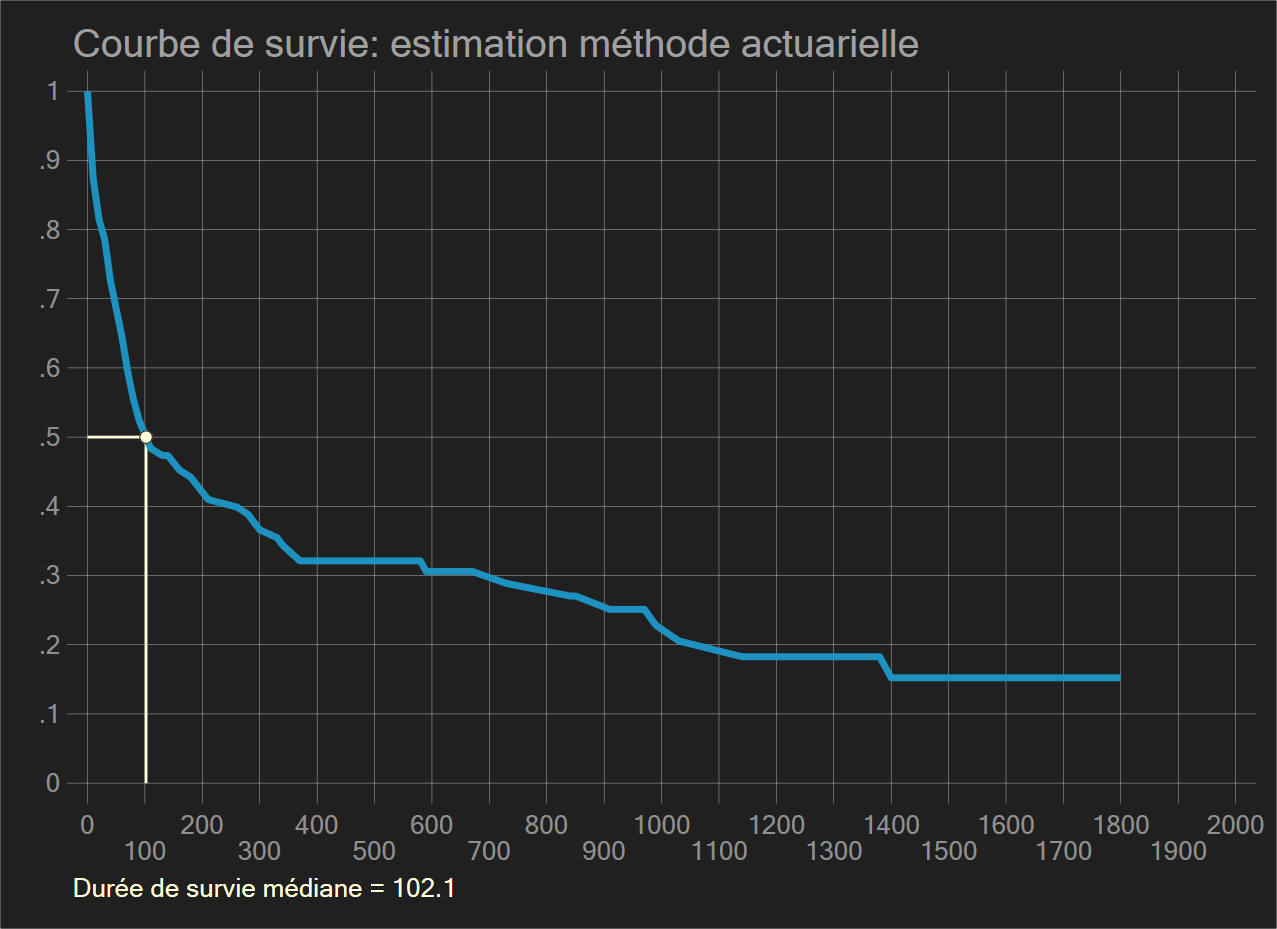
\includegraphics[width=0.7\textwidth,height=\textheight]{images/Image7.png}

}

\end{figure}

Lecture des résultats: 102 jours après leur inscription dans le registre
d'attente pour une greffe, 50\% des malades sont toujours en vie. Au
bout de 914 jours, 75\% sont décédés.

\hypertarget{la-muxe9thode-de-kaplan-meier}{%
\section{\texorpdfstring{\textbf{La méthode de
Kaplan-Meier}}{La méthode de Kaplan-Meier}}\label{la-muxe9thode-de-kaplan-meier}}

\begin{itemize}
\tightlist
\item
  L'approche qui exploite toute l'information disponible est celle dite
  de \textbf{Kaplan-Meier} (\emph{KM}).
\item
  Il y a autant d'intervalles que de durées où l'on observe au moins un
  évènement.
\item
  Au lieu d'utiliser des intervalles prédéterminés, l'estimateur KM va
  définir un intervalle entre chaque évènement enregistré.
\item
  La fonction de survie estimée par la méthode KM est une fonction en
  escalier (stairstep), d'où une estimation dite ``discrète''.
\item
  Pour chaque intervalle, on compte le nombe d'évènements et le nombre
  de censures.
\item
  Méthode adaptée pour une mesure de la durée de type continue.
\end{itemize}

\hypertarget{estimation-1}{%
\subsection{Estimation}\label{estimation-1}}

\textbf{Définition du Risk Set (}\(r_i\))

S'il y a à la fois des évènements et des censures à une durée \(t_i\),
les observations censurées sont considérées comme exposées au risque à
ce moment, comme si elles étaient censurées très rapidement après. C'est
la principale caractéristique de cette méthode, appelé également
l'estimateur \textbf{\emph{product-limit}}

\[r_i=r_{i-1}-d_{i-1}-c_{i-1}\]\\

\textbf{Calcul de} \(q_i\)\\
On applique la méthode de la section précédente avec:

\[q_i=\frac{d_i}{r_{i-1}-d_{i-1}-c_{i-1}}\] \emph{Remarque}: la variance
de l'estimateur est obtenu par la méthode dite de \emph{Greenwood}. Il
n'y a pas d'intérêt particulier de la décrire dans ce support.

\textbf{Récupération de la médiane}\\
Il n'y a pas de méthode pour calculer directement la durée médiane (ou
tout autre quantile) contrairement à l'approche actuarielle.\\
La définition retenue est conventionnelle. On va prendre la valeur de la
durée qui se situe juste \textbf{en dessous} de 50\% de survivant.e.s.
Elle est donc définie tel que \(S(t)\leq0.5\). Attention, il n'est pas
impossible que le \% de survivant.e.s soit bien en deçà de 50\% pour
l'obtention cette durée médiane.

\textbf{R-Stata-Sas-Python}

\subsection{R}

Les estimateurs sont obtenus avec fonction \textbf{\texttt{survfit}} du
package \texttt{survival}. On peut obtenir des rendus graphiques de
meilleures qualité avec le package \texttt{survminer} (fonction
\texttt{ggsurvplot})

\subsection{Stata}

Après avoir appelé les variables de durée et de censure en mode
\textbf{survival} avec \textbf{\texttt{stset}}), le tableau des
estimateurs est obtenu avec la commande \textbf{\texttt{sts\ list}} et
le graphique avec \textbf{\texttt{sts\ graph}}.

\subsection{SAS}

L'estimation de Kaplan-Meier est affichée par défaut par la
\texttt{proc\ lifetest}. \textbf{\emph{Warning}} : le tableau affiché
par SAS est particulièrement pénible à lire voire illisible, en
particulier lorsque le nombre de censures est élevé, une ligne étant
ajoutée pour chaque observation censurée. Je conseille de ne pas
afficher cette partie de l'output (se reporter à la section SAS du
chapitre programmation). On récupère pour le reste de l'output les
valeurs de la durée pour S(t) =(.75,.5,.25) ainsi que le graphique, ce
qui est suffisant.

\subsection{Python}

Les resultats sont donnés dans la librairie \texttt{lifeline} par des
fonctions au nom interminable. Je conseille plutôt l'utilisation de la
librairie \textbf{\texttt{statmodels}} (se reporter à la section dédiée
à Python).

\hypertarget{application-1}{%
\subsection{Application}\label{application-1}}

On reprend l'exemple précédent.

\begin{Shaded}
\begin{Highlighting}[]
\NormalTok{Time    Total   Fail   Lost           Function     Error     [}\DecValTok{95}\NormalTok{\% Conf. Int.]}
\SpecialCharTok{{-}{-}{-}{-}{-}{-}{-}{-}{-}{-}{-}{-}{-}{-}{-}{-}{-}{-}{-}{-}{-}{-}{-}{-}{-}{-}{-}{-}{-}{-}{-}{-}{-}{-}{-}{-}{-}{-}{-}{-}{-}{-}{-}{-}{-}{-}{-}{-}{-}{-}{-}{-}{-}{-}{-}{-}{-}{-}{-}{-}{-}{-}{-}{-}{-}{-}{-}{-}{-}{-}{-}{-}{-}{-}{-}{-}{-}{-}{-}}
     \DecValTok{1}      \DecValTok{103}      \DecValTok{1}      \DecValTok{0}             \FloatTok{0.9903}    \FloatTok{0.0097}     \FloatTok{0.9331}    \FloatTok{0.9986}
     \DecValTok{2}      \DecValTok{102}      \DecValTok{3}      \DecValTok{0}             \FloatTok{0.9612}    \FloatTok{0.0190}     \FloatTok{0.8998}    \FloatTok{0.9852}
     \DecValTok{3}       \DecValTok{99}      \DecValTok{3}      \DecValTok{0}             \FloatTok{0.9320}    \FloatTok{0.0248}     \FloatTok{0.8627}    \FloatTok{0.9670}
     \DecValTok{5}       \DecValTok{96}      \DecValTok{2}      \DecValTok{0}             \FloatTok{0.9126}    \FloatTok{0.0278}     \FloatTok{0.8388}    \FloatTok{0.9535}
     \DecValTok{6}       \DecValTok{94}      \DecValTok{2}      \DecValTok{0}             \FloatTok{0.8932}    \FloatTok{0.0304}     \FloatTok{0.8155}    \FloatTok{0.9394}
     \DecValTok{8}       \DecValTok{92}      \DecValTok{1}      \DecValTok{0}             \FloatTok{0.8835}    \FloatTok{0.0316}     \FloatTok{0.8040}    \FloatTok{0.9321}
     \DecValTok{9}       \DecValTok{91}      \DecValTok{1}      \DecValTok{0}             \FloatTok{0.8738}    \FloatTok{0.0327}     \FloatTok{0.7926}    \FloatTok{0.9247}
    \DecValTok{11}       \DecValTok{90}      \DecValTok{0}      \DecValTok{1}             \FloatTok{0.8738}    \FloatTok{0.0327}     \FloatTok{0.7926}    \FloatTok{0.9247}
    \DecValTok{12}       \DecValTok{89}      \DecValTok{1}      \DecValTok{0}             \FloatTok{0.8640}    \FloatTok{0.0338}     \FloatTok{0.7811}    \FloatTok{0.9171}
    \DecValTok{16}       \DecValTok{88}      \DecValTok{3}      \DecValTok{0}             \FloatTok{0.8345}    \FloatTok{0.0367}     \FloatTok{0.7474}    \FloatTok{0.8937}
    \DecValTok{17}       \DecValTok{85}      \DecValTok{1}      \DecValTok{0}             \FloatTok{0.8247}    \FloatTok{0.0375}     \FloatTok{0.7363}    \FloatTok{0.8857}
    \DecValTok{18}       \DecValTok{84}      \DecValTok{1}      \DecValTok{0}             \FloatTok{0.8149}    \FloatTok{0.0383}     \FloatTok{0.7253}    \FloatTok{0.8777}
    \DecValTok{21}       \DecValTok{83}      \DecValTok{2}      \DecValTok{0}             \FloatTok{0.7952}    \FloatTok{0.0399}     \FloatTok{0.7034}    \FloatTok{0.8614}
    \DecValTok{28}       \DecValTok{81}      \DecValTok{1}      \DecValTok{0}             \FloatTok{0.7854}    \FloatTok{0.0406}     \FloatTok{0.6926}    \FloatTok{0.8531}
    \DecValTok{30}       \DecValTok{80}      \DecValTok{1}      \DecValTok{0}             \FloatTok{0.7756}    \FloatTok{0.0412}     \FloatTok{0.6819}    \FloatTok{0.8448}
    \DecValTok{31}       \DecValTok{79}      \DecValTok{0}      \DecValTok{1}             \FloatTok{0.7756}    \FloatTok{0.0412}     \FloatTok{0.6819}    \FloatTok{0.8448}
    \DecValTok{32}       \DecValTok{78}      \DecValTok{1}      \DecValTok{0}             \FloatTok{0.7657}    \FloatTok{0.0419}     \FloatTok{0.6710}    \FloatTok{0.8363}
    \DecValTok{35}       \DecValTok{77}      \DecValTok{1}      \DecValTok{0}             \FloatTok{0.7557}    \FloatTok{0.0425}     \FloatTok{0.6603}    \FloatTok{0.8278}
    \DecValTok{36}       \DecValTok{76}      \DecValTok{1}      \DecValTok{0}             \FloatTok{0.7458}    \FloatTok{0.0431}     \FloatTok{0.6495}    \FloatTok{0.8192}
    \DecValTok{37}       \DecValTok{75}      \DecValTok{1}      \DecValTok{0}             \FloatTok{0.7358}    \FloatTok{0.0436}     \FloatTok{0.6388}    \FloatTok{0.8106}
    \DecValTok{39}       \DecValTok{74}      \DecValTok{1}      \DecValTok{1}             \FloatTok{0.7259}    \FloatTok{0.0442}     \FloatTok{0.6282}    \FloatTok{0.8019}
    \DecValTok{40}       \DecValTok{72}      \DecValTok{2}      \DecValTok{0}             \FloatTok{0.7057}    \FloatTok{0.0452}     \FloatTok{0.6068}    \FloatTok{0.7842}
    \DecValTok{43}       \DecValTok{70}      \DecValTok{1}      \DecValTok{0}             \FloatTok{0.6956}    \FloatTok{0.0457}     \FloatTok{0.5961}    \FloatTok{0.7752}
    \DecValTok{45}       \DecValTok{69}      \DecValTok{1}      \DecValTok{0}             \FloatTok{0.6856}    \FloatTok{0.0461}     \FloatTok{0.5855}    \FloatTok{0.7662}
    \DecValTok{50}       \DecValTok{68}      \DecValTok{1}      \DecValTok{0}             \FloatTok{0.6755}    \FloatTok{0.0465}     \FloatTok{0.5750}    \FloatTok{0.7572}
    \DecValTok{51}       \DecValTok{67}      \DecValTok{1}      \DecValTok{0}             \FloatTok{0.6654}    \FloatTok{0.0469}     \FloatTok{0.5645}    \FloatTok{0.7481}
    \DecValTok{53}       \DecValTok{66}      \DecValTok{1}      \DecValTok{0}             \FloatTok{0.6553}    \FloatTok{0.0472}     \FloatTok{0.5541}    \FloatTok{0.7390}
    \DecValTok{58}       \DecValTok{65}      \DecValTok{1}      \DecValTok{0}             \FloatTok{0.6452}    \FloatTok{0.0476}     \FloatTok{0.5437}    \FloatTok{0.7298}
    \DecValTok{61}       \DecValTok{64}      \DecValTok{1}      \DecValTok{0}             \FloatTok{0.6352}    \FloatTok{0.0479}     \FloatTok{0.5333}    \FloatTok{0.7206}
    \DecValTok{66}       \DecValTok{63}      \DecValTok{1}      \DecValTok{0}             \FloatTok{0.6251}    \FloatTok{0.0482}     \FloatTok{0.5230}    \FloatTok{0.7113}
    \DecValTok{68}       \DecValTok{62}      \DecValTok{2}      \DecValTok{0}             \FloatTok{0.6049}    \FloatTok{0.0487}     \FloatTok{0.5026}    \FloatTok{0.6926}
    \DecValTok{69}       \DecValTok{60}      \DecValTok{1}      \DecValTok{0}             \FloatTok{0.5948}    \FloatTok{0.0489}     \FloatTok{0.4924}    \FloatTok{0.6832}
    \DecValTok{72}       \DecValTok{59}      \DecValTok{2}      \DecValTok{0}             \FloatTok{0.5747}    \FloatTok{0.0493}     \FloatTok{0.4722}    \FloatTok{0.6643}
    \DecValTok{77}       \DecValTok{57}      \DecValTok{1}      \DecValTok{0}             \FloatTok{0.5646}    \FloatTok{0.0494}     \FloatTok{0.4621}    \FloatTok{0.6548}
    \DecValTok{78}       \DecValTok{56}      \DecValTok{1}      \DecValTok{0}             \FloatTok{0.5545}    \FloatTok{0.0496}     \FloatTok{0.4521}    \FloatTok{0.6453}
    \DecValTok{80}       \DecValTok{55}      \DecValTok{1}      \DecValTok{0}             \FloatTok{0.5444}    \FloatTok{0.0497}     \FloatTok{0.4422}    \FloatTok{0.6357}
    \DecValTok{81}       \DecValTok{54}      \DecValTok{1}      \DecValTok{0}             \FloatTok{0.5343}    \FloatTok{0.0498}     \FloatTok{0.4323}    \FloatTok{0.6261}
    \DecValTok{85}       \DecValTok{53}      \DecValTok{1}      \DecValTok{0}             \FloatTok{0.5243}    \FloatTok{0.0499}     \FloatTok{0.4224}    \FloatTok{0.6164}
    \DecValTok{90}       \DecValTok{52}      \DecValTok{1}      \DecValTok{0}             \FloatTok{0.5142}    \FloatTok{0.0499}     \FloatTok{0.4125}    \FloatTok{0.6067}
    \DecValTok{96}       \DecValTok{51}      \DecValTok{1}      \DecValTok{0}             \FloatTok{0.5041}    \FloatTok{0.0499}     \FloatTok{0.4027}    \FloatTok{0.5969}
   \DecValTok{100}       \DecValTok{50}      \DecValTok{1}      \DecValTok{0}             \FloatTok{0.4940}    \FloatTok{0.0499}     \FloatTok{0.3930}    \FloatTok{0.5872}
   \DecValTok{102}       \DecValTok{49}      \DecValTok{1}      \DecValTok{0}             \FloatTok{0.4839}    \FloatTok{0.0499}     \FloatTok{0.3833}    \FloatTok{0.5773}
   \DecValTok{109}       \DecValTok{48}      \DecValTok{0}      \DecValTok{1}             \FloatTok{0.4839}    \FloatTok{0.0499}     \FloatTok{0.3833}    \FloatTok{0.5773}
   \DecValTok{110}       \DecValTok{47}      \DecValTok{1}      \DecValTok{0}             \FloatTok{0.4736}    \FloatTok{0.0499}     \FloatTok{0.3733}    \FloatTok{0.5673}
   \DecValTok{131}       \DecValTok{46}      \DecValTok{0}      \DecValTok{1}             \FloatTok{0.4736}    \FloatTok{0.0499}     \FloatTok{0.3733}    \FloatTok{0.5673}
   \DecValTok{149}       \DecValTok{45}      \DecValTok{1}      \DecValTok{0}             \FloatTok{0.4631}    \FloatTok{0.0499}     \FloatTok{0.3632}    \FloatTok{0.5571}
   \DecValTok{153}       \DecValTok{44}      \DecValTok{1}      \DecValTok{0}             \FloatTok{0.4526}    \FloatTok{0.0499}     \FloatTok{0.3531}    \FloatTok{0.5468}
   \DecValTok{165}       \DecValTok{43}      \DecValTok{1}      \DecValTok{0}             \FloatTok{0.4421}    \FloatTok{0.0498}     \FloatTok{0.3430}    \FloatTok{0.5364}
   \DecValTok{180}       \DecValTok{42}      \DecValTok{0}      \DecValTok{1}             \FloatTok{0.4421}    \FloatTok{0.0498}     \FloatTok{0.3430}    \FloatTok{0.5364}
   \DecValTok{186}       \DecValTok{41}      \DecValTok{1}      \DecValTok{0}             \FloatTok{0.4313}    \FloatTok{0.0497}     \FloatTok{0.3327}    \FloatTok{0.5258}
   \DecValTok{188}       \DecValTok{40}      \DecValTok{1}      \DecValTok{0}             \FloatTok{0.4205}    \FloatTok{0.0497}     \FloatTok{0.3225}    \FloatTok{0.5152}
   \DecValTok{207}       \DecValTok{39}      \DecValTok{1}      \DecValTok{0}             \FloatTok{0.4097}    \FloatTok{0.0495}     \FloatTok{0.3123}    \FloatTok{0.5045}
   \DecValTok{219}       \DecValTok{38}      \DecValTok{1}      \DecValTok{0}             \FloatTok{0.3989}    \FloatTok{0.0494}     \FloatTok{0.3022}    \FloatTok{0.4938}
   \DecValTok{263}       \DecValTok{37}      \DecValTok{1}      \DecValTok{0}             \FloatTok{0.3881}    \FloatTok{0.0492}     \FloatTok{0.2921}    \FloatTok{0.4830}
   \DecValTok{265}       \DecValTok{36}      \DecValTok{0}      \DecValTok{1}             \FloatTok{0.3881}    \FloatTok{0.0492}     \FloatTok{0.2921}    \FloatTok{0.4830}
   \DecValTok{285}       \DecValTok{35}      \DecValTok{2}      \DecValTok{0}             \FloatTok{0.3660}    \FloatTok{0.0488}     \FloatTok{0.2714}    \FloatTok{0.4608}
   \DecValTok{308}       \DecValTok{33}      \DecValTok{1}      \DecValTok{0}             \FloatTok{0.3549}    \FloatTok{0.0486}     \FloatTok{0.2612}    \FloatTok{0.4496}
   \DecValTok{334}       \DecValTok{32}      \DecValTok{1}      \DecValTok{0}             \FloatTok{0.3438}    \FloatTok{0.0483}     \FloatTok{0.2510}    \FloatTok{0.4383}
   \DecValTok{340}       \DecValTok{31}      \DecValTok{1}      \DecValTok{1}             \FloatTok{0.3327}    \FloatTok{0.0480}     \FloatTok{0.2409}    \FloatTok{0.4270}
   \DecValTok{342}       \DecValTok{29}      \DecValTok{1}      \DecValTok{0}             \FloatTok{0.3212}    \FloatTok{0.0477}     \FloatTok{0.2305}    \FloatTok{0.4153}
   \DecValTok{370}       \DecValTok{28}      \DecValTok{0}      \DecValTok{1}             \FloatTok{0.3212}    \FloatTok{0.0477}     \FloatTok{0.2305}    \FloatTok{0.4153}
   \DecValTok{397}       \DecValTok{27}      \DecValTok{0}      \DecValTok{1}             \FloatTok{0.3212}    \FloatTok{0.0477}     \FloatTok{0.2305}    \FloatTok{0.4153}
   \DecValTok{427}       \DecValTok{26}      \DecValTok{0}      \DecValTok{1}             \FloatTok{0.3212}    \FloatTok{0.0477}     \FloatTok{0.2305}    \FloatTok{0.4153}
   \DecValTok{445}       \DecValTok{25}      \DecValTok{0}      \DecValTok{1}             \FloatTok{0.3212}    \FloatTok{0.0477}     \FloatTok{0.2305}    \FloatTok{0.4153}
   \DecValTok{482}       \DecValTok{24}      \DecValTok{0}      \DecValTok{1}             \FloatTok{0.3212}    \FloatTok{0.0477}     \FloatTok{0.2305}    \FloatTok{0.4153}
   \DecValTok{515}       \DecValTok{23}      \DecValTok{0}      \DecValTok{1}             \FloatTok{0.3212}    \FloatTok{0.0477}     \FloatTok{0.2305}    \FloatTok{0.4153}
   \DecValTok{545}       \DecValTok{22}      \DecValTok{0}      \DecValTok{1}             \FloatTok{0.3212}    \FloatTok{0.0477}     \FloatTok{0.2305}    \FloatTok{0.4153}
   \DecValTok{583}       \DecValTok{21}      \DecValTok{1}      \DecValTok{0}             \FloatTok{0.3059}    \FloatTok{0.0478}     \FloatTok{0.2156}    \FloatTok{0.4008}
   \DecValTok{596}       \DecValTok{20}      \DecValTok{0}      \DecValTok{1}             \FloatTok{0.3059}    \FloatTok{0.0478}     \FloatTok{0.2156}    \FloatTok{0.4008}
   \DecValTok{620}       \DecValTok{19}      \DecValTok{0}      \DecValTok{1}             \FloatTok{0.3059}    \FloatTok{0.0478}     \FloatTok{0.2156}    \FloatTok{0.4008}
   \DecValTok{670}       \DecValTok{18}      \DecValTok{0}      \DecValTok{1}             \FloatTok{0.3059}    \FloatTok{0.0478}     \FloatTok{0.2156}    \FloatTok{0.4008}
   \DecValTok{675}       \DecValTok{17}      \DecValTok{1}      \DecValTok{0}             \FloatTok{0.2879}    \FloatTok{0.0483}     \FloatTok{0.1976}    \FloatTok{0.3844}
   \DecValTok{733}       \DecValTok{16}      \DecValTok{1}      \DecValTok{0}             \FloatTok{0.2699}    \FloatTok{0.0485}     \FloatTok{0.1802}    \FloatTok{0.3676}
   \DecValTok{841}       \DecValTok{15}      \DecValTok{0}      \DecValTok{1}             \FloatTok{0.2699}    \FloatTok{0.0485}     \FloatTok{0.1802}    \FloatTok{0.3676}
   \DecValTok{852}       \DecValTok{14}      \DecValTok{1}      \DecValTok{0}             \FloatTok{0.2507}    \FloatTok{0.0487}     \FloatTok{0.1616}    \FloatTok{0.3497}
   \DecValTok{915}       \DecValTok{13}      \DecValTok{0}      \DecValTok{1}             \FloatTok{0.2507}    \FloatTok{0.0487}     \FloatTok{0.1616}    \FloatTok{0.3497}
   \DecValTok{941}       \DecValTok{12}      \DecValTok{0}      \DecValTok{1}             \FloatTok{0.2507}    \FloatTok{0.0487}     \FloatTok{0.1616}    \FloatTok{0.3497}
   \DecValTok{979}       \DecValTok{11}      \DecValTok{1}      \DecValTok{0}             \FloatTok{0.2279}    \FloatTok{0.0493}     \FloatTok{0.1394}    \FloatTok{0.3295}
   \DecValTok{995}       \DecValTok{10}      \DecValTok{1}      \DecValTok{0}             \FloatTok{0.2051}    \FloatTok{0.0494}     \FloatTok{0.1183}    \FloatTok{0.3085}

\NormalTok{[Résultats non reportés à partir de t}\OtherTok{=}\DecValTok{1000}\NormalTok{ ]}
\SpecialCharTok{{-}{-}{-}{-}{-}{-}{-}{-}{-}{-}{-}{-}{-}{-}{-}{-}{-}{-}{-}{-}{-}{-}{-}{-}{-}{-}{-}{-}{-}{-}{-}{-}{-}{-}{-}{-}{-}{-}{-}{-}{-}{-}{-}{-}{-}{-}{-}{-}{-}{-}{-}{-}{-}{-}{-}{-}{-}{-}{-}{-}{-}{-}{-}{-}{-}{-}{-}{-}{-}{-}{-}{-}{-}{-}{-}{-}{-}{-}{-}}
\end{Highlighting}
\end{Shaded}

La durée durée médiane de survie est \(t=100\). Elle correspond à
\(S(t)=0.4940\).

\begin{longtable}[]{@{}ll@{}}
\caption{Quantiles de la fonction de séjour type
Kaplan-Meier}\tabularnewline
\toprule\noalign{}
\textbf{S(t)} & \textbf{t} \\
\midrule\noalign{}
\endfirsthead
\toprule\noalign{}
\textbf{S(t)} & \textbf{t} \\
\midrule\noalign{}
\endhead
\bottomrule\noalign{}
\endlastfoot
0.90 & 6 \\
0.75 & 36 \\
0.50 & 100 \\
0.25 & 979 \\
0.1 & . \\
\end{longtable}

\begin{figure}

\caption{Courbe de survie: estimation méthode actuarielle}

{\centering 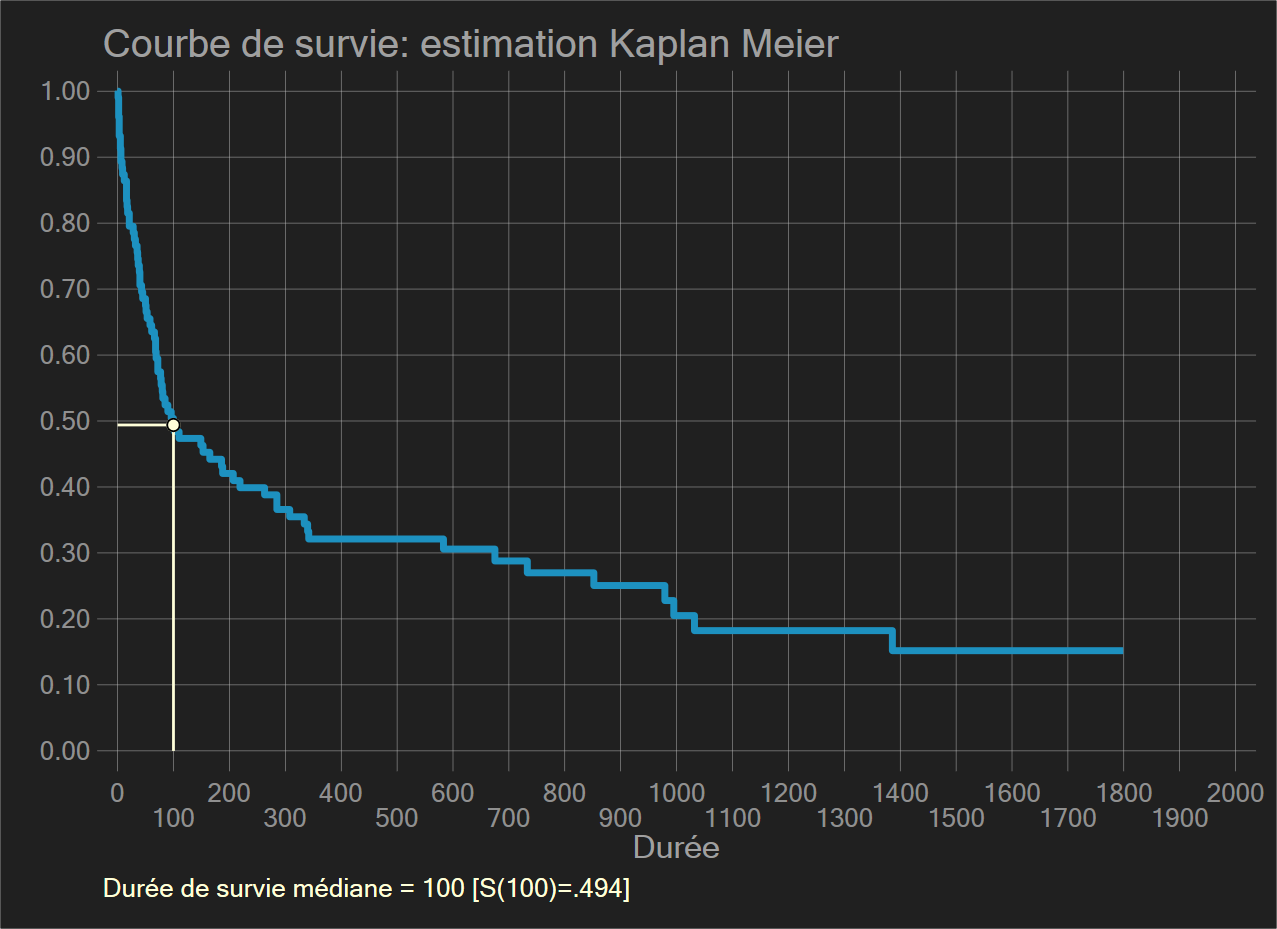
\includegraphics[width=0.7\textwidth,height=\textheight]{images/Image8.png}

}

\end{figure}

\begin{figure}

\caption{Courbe de survie: estimation méthode actuarielle + CI}

{\centering 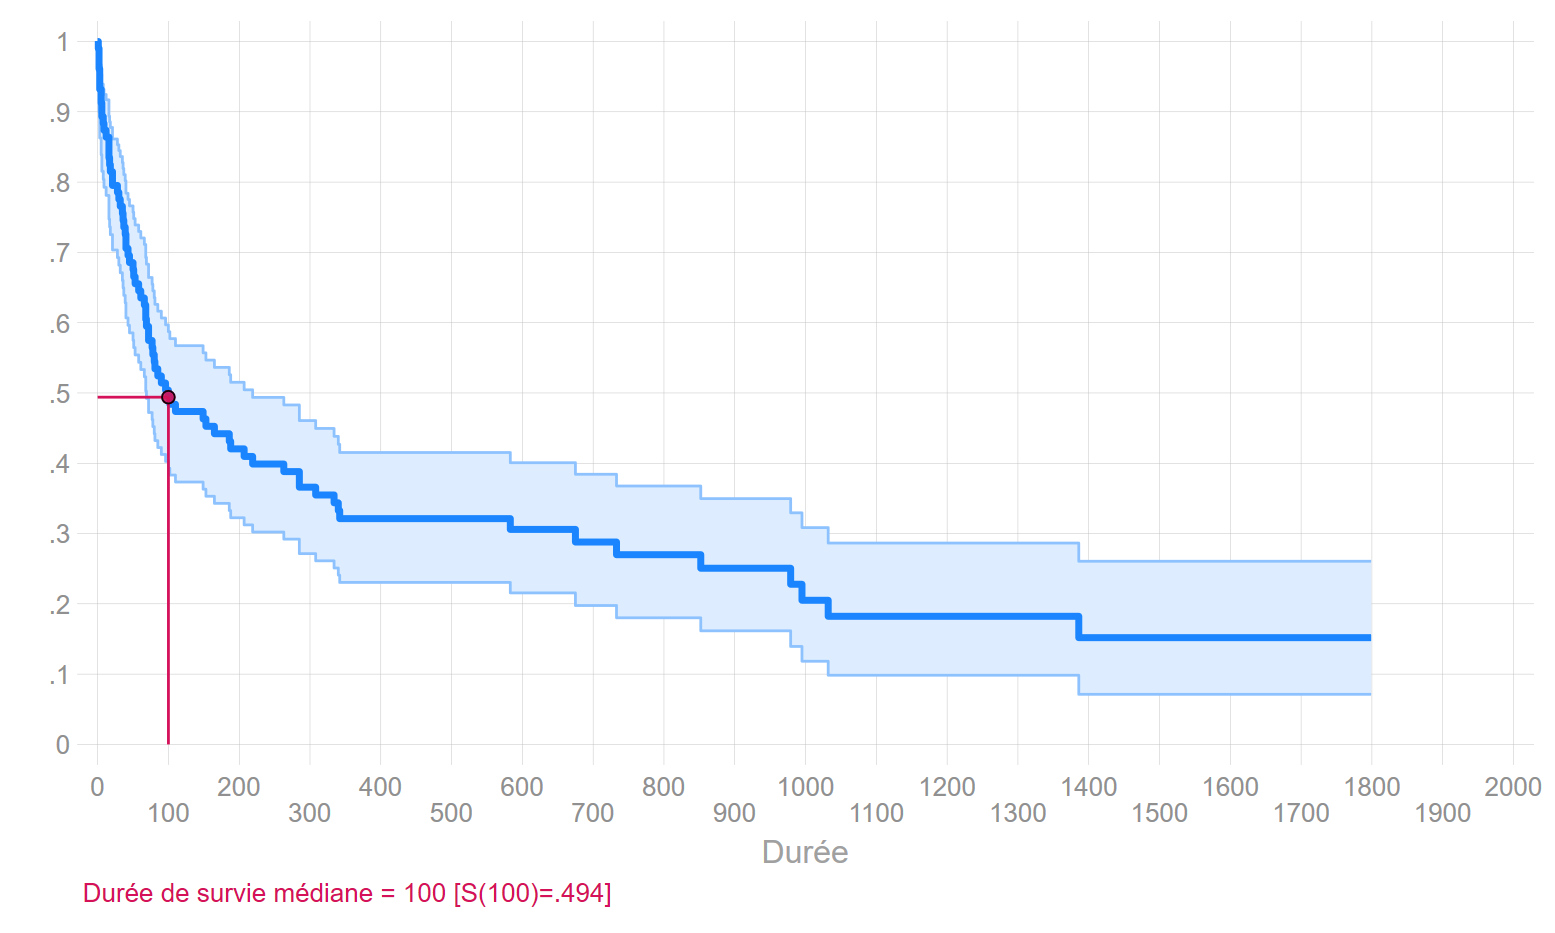
\includegraphics[width=0.7\textwidth,height=\textheight]{images/Image8b.png}

}

\end{figure}

\hypertarget{quantituxe9s-associuxe9es-uxe0-lestimateur-kaplan-meier..}{%
\subsection{Quantités associées à l'estimateur
Kaplan-Meier..}\label{quantituxe9s-associuxe9es-uxe0-lestimateur-kaplan-meier..}}

\textbf{Le risque cumulé}: estimateur de Nelson AAlen

Il est simplément égal à:

\[H(t)=\sum_{t_i\leq k}q(t_i)\]

\begin{figure}

\caption{Risque cumulé: estimateur Nelson-Aalen}

{\centering 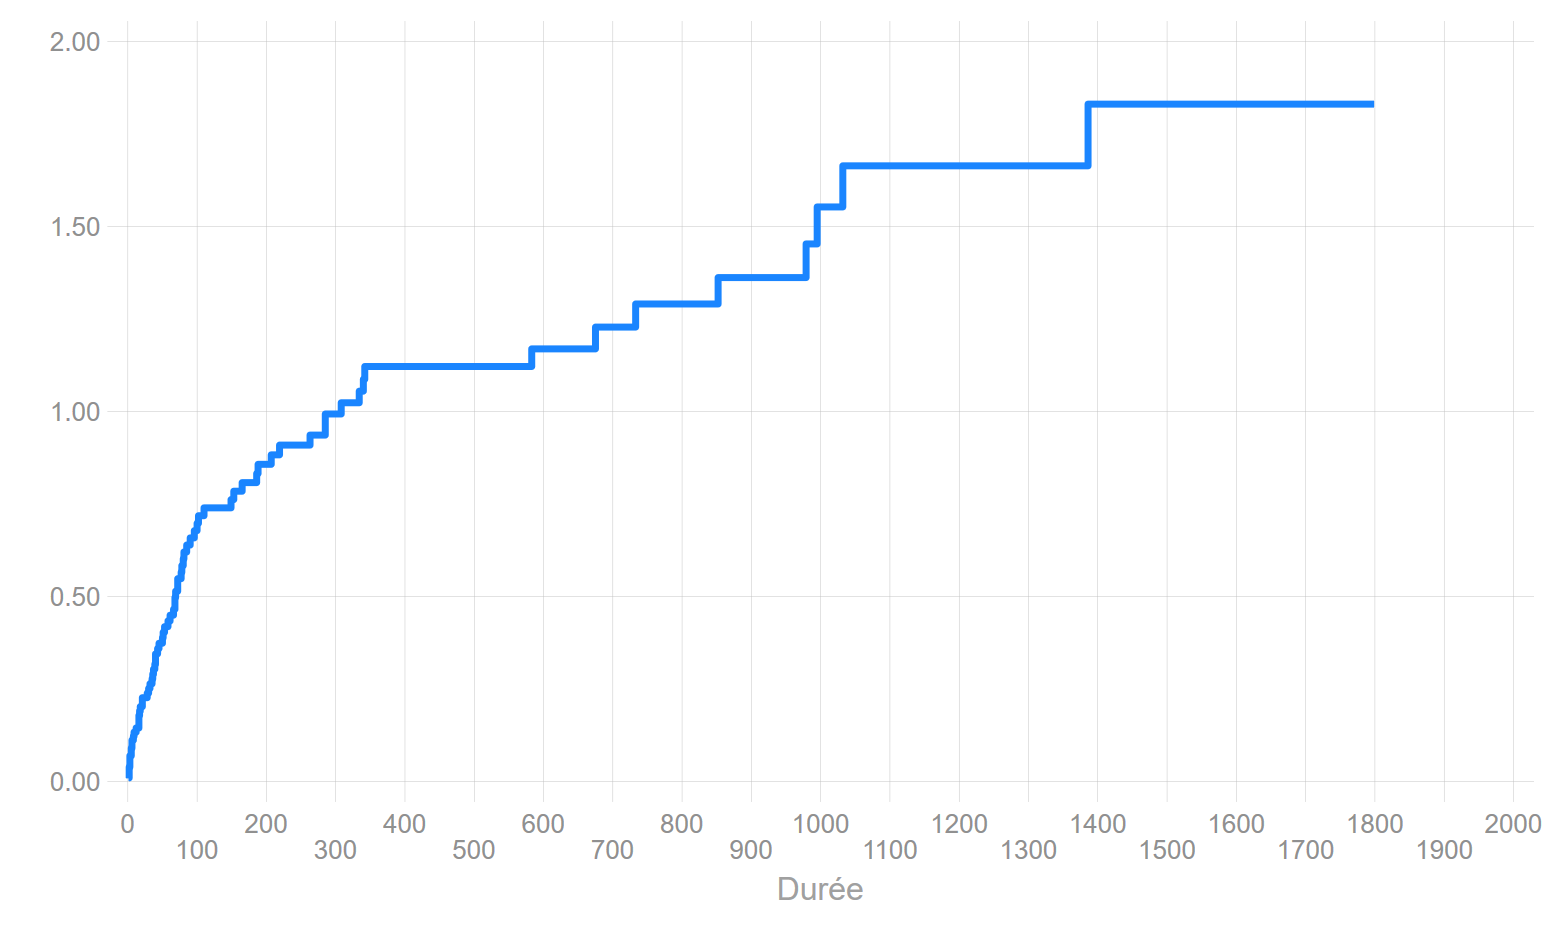
\includegraphics[width=0.7\textwidth,height=\textheight]{images/Image19.png}

}

\end{figure}

\textbf{Le risque instantané}

Nécessite l'estimateur de risque cumulé de Nelson-Aalen. Le risque est
obtenu en lissant les différences - toujours positive - entre \(H(t)\)
par la méthode dite du \textbf{kernel} (cf estimation de la densité des
distributions). Elle permet d'obtenir une fonction continue avec la
durée (paramétrables sur les largeurs des fenêtres de lissage). D'autres
méthodes de lissage sont maintenant possibles, et de plus en plus
utilisées, en particulier celles utilisant des splines.

\begin{figure}

\caption{Risque instantané: estimateur du Kernel}

{\centering 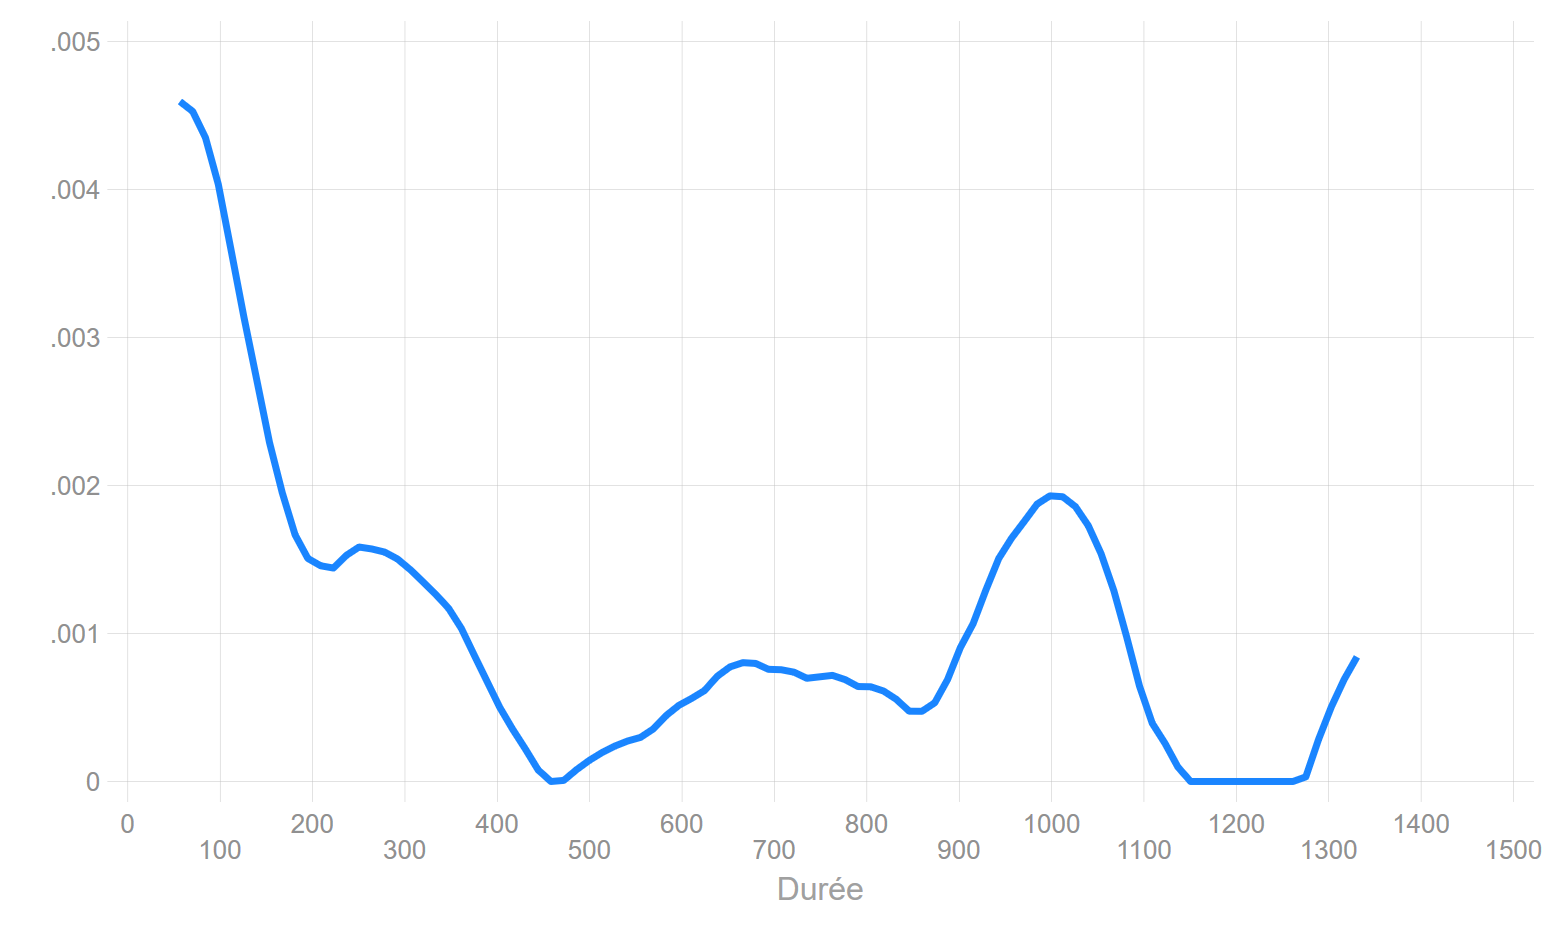
\includegraphics[width=0.7\textwidth,height=\textheight]{images/Image20.png}

}

\end{figure}

\begin{tcolorbox}[enhanced jigsaw, arc=.35mm, bottomrule=.15mm, titlerule=0mm, colbacktitle=quarto-callout-note-color!10!white, left=2mm, opacitybacktitle=0.6, toprule=.15mm, title=\textcolor{quarto-callout-note-color}{\faInfo}\hspace{0.5em}{Note}, colframe=quarto-callout-note-color-frame, breakable, coltitle=black, opacityback=0, toptitle=1mm, bottomtitle=1mm, rightrule=.15mm, leftrule=.75mm, colback=white]

Il n'est pas inutile de noter qu'il n'y a pas de \emph{formule} toute
faite pour obtenir des valeurs du risque instantané. Ce type de méthode
par lissage est pleinement paramétrable, par exemple sa fenêtre, ce qui
implique que son profil varie d'un paramétrage à l'autre. Le graphique
précédent a été fait avec Stata, si on utilisait le package
\texttt{muhaz} les différences de paramétrage par défaut font que les
courbes ne se confondent pas.

\end{tcolorbox}

\hypertarget{tests-de-comparaison}{%
\chapter{\texorpdfstring{\textbf{Tests de
comparaison}}{Tests de comparaison}}\label{tests-de-comparaison}}

\begin{itemize}
\tightlist
\item
  Les tests d'égalités des fonctions de survie entre différentes valeurs
  d'une covariable sont calculés à partir de la méthode de Kaplan Meier.
\item
  L'utilisation du test correspond à la nécessité de déterminer si une
  même distribution gouverne les évènements observés dans les
  différentes strates.\\
\item
  \textbf{Attention}: pas de test possible sur des variables
  quantitatives. Il faut donc prévoir des regroupements pour les
  transformer en variable ordinale.
\end{itemize}

Deux méthodes sont utilisées:

\begin{itemize}
\tightlist
\item
  La plus ancienne, la plus diffusée, et peut-être la moins bonne: test
  dits du \textbf{log-rank}).
\item
  Plus récente et (hélas) moins difusée: comparaison des \textbf{RMST}
  (\emph{Restricted Mean of Survival Time}).
\end{itemize}

\hypertarget{tests-du-log-rank}{%
\section{Tests du log-rank}\label{tests-du-log-rank}}

Il s'agit d'une série de tests qui répondent à la même logique, la seule
différence réside dans le poids accordé au début ou à la fin de la
période d'observation. Par ailleurs ces différents tests sont plus ou
moins sensibles à la distribution des censures à droites entre les sous
échantillons et à la non proportionalité des risques.

Dans leur logique, ces tests entrent dans le cadre des tests
d'indépendance du Khi2, même si formellement ils relèvent des techniques
dites de rang.\\
Il s'agira donc de comparer des effectifs observés à des effectifs
espérés à chaque moment d'évènement. La principale différence réside
dans le calcul de la variance de la statistique du test qui, ici, suit
assez logiquement une loi hypergéométrique {[}proche loi binomiale mais
avec tirage avec remise{]}.

\hypertarget{principe-de-calcul-de-la-statistique-de-test}{%
\subsection{Principe de calcul de la statistique de
test}\label{principe-de-calcul-de-la-statistique-de-test}}

\begin{itemize}
\tightlist
\item
  \textbf{Effectifs observés en \(t_i\)}: \(o_{i1}\) et \(o_{i2}\) sont
  égaux à \(d_{i1}\) et \(d_{i2}\), et leur somme pour tous les temps
  d'évènement à \(O_1\) et \(O_2\).
\item
  \textbf{Effectifs expérés} (hypothèse nulle \(H_0\)): comme pour une
  statistique du \(\chi^2\) on se base sur les marges, avec le risque
  set (\(R_i\)) en \(t_i\) pour dénombrer les effectifs, soit
  \(e_{i1}=R_{i1}\times\frac{d_i}{R_i}\) et
  \(e_{i2}=R_{i2}\times\frac{d_2}{R_i}\). Leur somme pour tous les temps
  d'évènement est égale à \(E_1\) et \(E_2\). Le principe de calcul des
  effectifs observés reposent donc sur l'hypothèse d'un rapport des
  risques toujours égal à 1 au cours du temps (\emph{hypothèse
  fondamentale de risques proportionnels}).
\item
  \textbf{Statistique du log-rank}: \((O_1 - E_1) = -(O_2 - E_2)\).
\item
  \textbf{Statistique de test}: sous \(H_0\),
  \(\frac{(O_1 - E_1)^2}{\sum{v_i}}\), avec \(v_i\) la variance de
  \((o_{i1} - e_{i2})\), suis un \(\chi^2(1)\). Si on teste
  simultanément la différence de \(g\) fonctions de survie, ce qui n'est
  pas une bonne idée en passant, la statistique de test suis un
  \(\chi^2(g-1)\).
\end{itemize}

\hypertarget{les-principaux-tests-log-rank}{%
\subsection{Les principaux tests
log-rank}\label{les-principaux-tests-log-rank}}

Le principe de construction des effectifs observés et espérés reste le
même dans chaque test, les différences résident dans les pondérations
(\(w_i\)) qui prennent en compte, de manière différente, la taille de la
population soumise au risque à chaque durée où au moins un évènement est
observé.

\begin{itemize}
\item
  \textbf{Test du log-rank}: \(w_i=1\)\\
  Il accorde le même poids à toutes les durées d'évènement. C'est le
  test standard, le plus utilisé.
\item
  \textbf{Test de Wilconxon-Breslow-Grehan}: \(w_i=R_i\)\\
  Les écarts entre effectifs observés et espérés sont pondérés par la
  population soumise à risque en \(t_i\). Le test accorde plus de poids
  au début de la période analysée, et il est sensible aux différences de
  distributions entre les strates des observations censurées.
\item
  \textbf{Test de Tarone-Ware}: \(w_i=\sqrt{R_i}\)\\
  Variante du test précédent, il atténue le poids accordé aux évènements
  au début de la période d'observation. Il est par ailleurs moins
  sensible au problème de la distribution des censures entre les
  strates.
\item
  \textbf{Test de Peto-Peto} : \(w_i=S_i\)\\
  La pondération est une variante de la fonction de survie KM (avec
  \(R_i=R_i+1\)). Le test n'est pas sensible au problème de distribution
  des censures.
\item
  \textbf{Test de Fleming-Harington}: \(w_i=(S_i)^p\times(1-S_i)^{q}\)
  avec \(0\leq{p}\leq{1}\) Il permet de paramétrer le poids accordé au
  début où à la fin de temps d'observation. Si \(p=q=0\) on retrouve le
  test de base non pondéré.
\end{itemize}

\textbf{En pratique/remarques}:

\begin{itemize}
\item
  Les tests du log-rank sont sensibles à l'hypothèse de risques
  proportionnels (voir \textbf{modèle semi-paramétrique de Cox}). En
  pratique si des courbes de séjours se croisent, il est fortement
  déconseillé de les utiliser. Cela ne signifie pas que si les courbes
  ne se croisent pas, l'hypothèse de proportionalité des risques est
  respectée : des rapports de risque peuvent au cours du temps
  s'intensifier, se réduire ou, le cas échant s'inverser, ce qui est
  typique d'un croisement.
\item
  Effectuer un test global (multiple/omnibus) sur un nombre important de
  groupes (ou \textgreater2) peut rendre le test très facilement
  significatif. Il peut être intéressant de tester des courbes deux à
  deux (idem qu'une régression avec covariable discrète), en conservant
  un seul degré de liberté. Des méthodes de correction du test multiple
  sont possibles ou disponibles si on utilise R.
\end{itemize}

\textbf{R-Stata-Sas-Python}

\subsection{R}

On utilise la fonction \textbf{\texttt{survdiff}} de la librairie
\texttt{survival}. Le résultat du test de Peto-Peto est affiché par
défaut (\texttt{rho=1}). Si on souhaite utiliser le test non pondéré, on
ajoute l'option \texttt{rho=0}. Pour obtenir le résultat d'un test
multiple corrigé (plus d'un degré de liberté), on peut utiliser la
fonction \textbf{\texttt{pairwise\_survdiff}} du package
\textbf{\texttt{survminer}}. Cette fonction permet également d'obtenir
des tests 2 à 2.

Je conseille de rester sur l'option \textbf{\emph{Peto-Peto}} et dans le
cas d'une variable à plus de deux modalités, d'utiliser la fonction de
\texttt{survminer} \textbf{\texttt{pairwise\_survdiff}}.

\subsection{Stata}

On utilise la commande \textbf{\texttt{sts\ test}} avec le nom de la
version du test: \texttt{peto}, \texttt{wilcoxon} . Sans préciser le nom
de la variante, le test non pondéré est exécuté.

\subsection{Sas}

Le test non pondéré et la version Wilcoxon sont données avec l'option
\textbf{\texttt{strata}} de la \texttt{proc\ lifetest}. Attention : ne
jamais utiliser la version \emph{LR Test} qui est biaisée. Pour obtenir
d'autres versions du test du log-rank, on ajoute
\textbf{\texttt{/test=all}} à l'option \texttt{strata}.

\subsection{Python}

Avec la librairie \texttt{lifelines}, on utilise la fonction
\textbf{\texttt{logrank\_test}}. Quatre variantes sont disponibles
(Wilcoxon, Tarone-Ware, Peto-Peto et Fleming-Harrigton). On peut
également utiliser la fonction \textbf{\texttt{duration.survdiff}} de
\texttt{statmodels} (non pondéré, Wilcoxon - appelé ici Breslow- et
Tarone-Ware).

\hypertarget{application-2}{%
\subsection{Application}\label{application-2}}

On compare ici l'effet du pontage coronarien sur le risque de décéder
depuis l'inscription dans le registre de greffe.

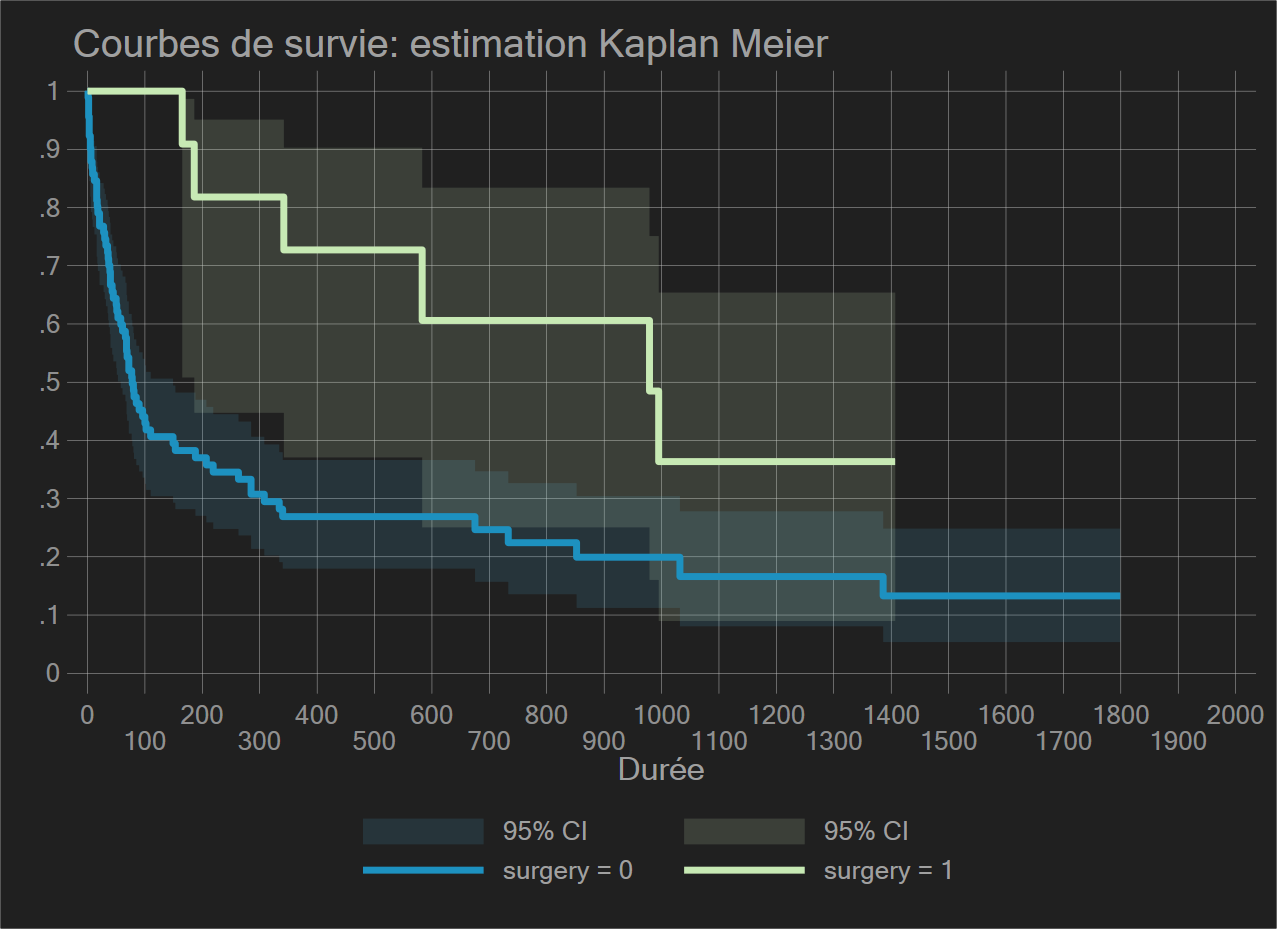
\includegraphics[width=0.7\textwidth,height=\textheight]{images/Image9.png}

\begin{longtable}[]{@{}llll@{}}
\caption{Résultats des tests du logrank}\tabularnewline
\toprule\noalign{}
\textbf{Test} & \textbf{df} & \textbf{Chi2} &
\textbf{P\textgreater Chi2} \\
\midrule\noalign{}
\endfirsthead
\toprule\noalign{}
\textbf{Test} & \textbf{df} & \textbf{Chi2} &
\textbf{P\textgreater Chi2} \\
\midrule\noalign{}
\endhead
\bottomrule\noalign{}
\endlastfoot
\textbf{Non pondéré} & 1 & 6.59 & 0.0103 \\
\textbf{Wilcoxon (Breslow}) & 1 & 8.99 & 0.0027 \\
\textbf{Tarone-Ware} & 1 & 8.46 & 0.0036 \\
\textbf{Peto-Peto} & & 8.66 & 0.0033 \\
\end{longtable}

Les résultats font apparaître que l'opération permet d'augmenter la
durée de survie des personnes. Il apparait que la p-value est plus
élevée pour test non pondérée. Cela peut-il s'expliquer en regardant les
deux courbes de séjours? Qu'en est-il de la proportionalité des risques
???? \ldots. Réponse pendant la formation.

\hypertarget{comparaison-des-rmst}{%
\section{Comparaison des RMST}\label{comparaison-des-rmst}}

\textbf{RMST}: \emph{Restricted Mean of Survival Time}

La comparaison des RMST est une alternative pertinente aux tests du
log-rank car elle ne repose pas sur des hypothèses contraignantes
(proportionnalité des risques, distribution des censures), et permet une
lecture vivante basée sur des espérances de séjour et non sur la lecture
d'une simple p-value traduisant l'homogénéité ou non des fonctions de
séjour. Par ailleurs les comparaisons sont souples, on peut choisir un
ou plusieurs points d'horizon pour alimenter l'analyse.

\textbf{Principe}

\begin{itemize}
\tightlist
\item
  L'aire sous la fonction de survie représente la durée moyenne
  d'attente jusqu'à l'évènement, soit une espérance de survie.
\item
  En présence de censure à droite, il faut borner la durée maximale
  \(t^*<\infty\). L'espérance de survie s'interprète donc sur un horizon
  fini. On est très proche d'une mesure en analyse démographique type «
  espérance de vie partielle ».
\item
  \(RMST =\int_0^{t^*}S(t)dt\).
\item
  On peut facilement comparer les RMST de deux groupes, en termes de
  différence ou de ratio.
\item
  Par défaut on définit généralement \(t^*\) à partir le temps du
  dernier évènement observé. Il est néanmoins possible de calculer le
  RMST sur des intervalles plus court, ce qui lui permet une véritable
  souplesse au niveau de l'analyse.
\end{itemize}

\textbf{R-Stata-Sas-Python}

Attention, selon les logiciels la durée max par défaut n'est pas la
même. Pour R et Sas, il s'agit du dernier évènement observé sur
l'ensemble de l'échantillon, alors que Stata prend la durée qui
correspond au dernier évènement observé le plus court des deux groupes .
Cela affectera légèrement la valeur des Rmst estimées par défaut.\\
Pour l'exemple, la durée maximale utilisée par R est de 1407 jours alors
que pour Stata elle est de 995 jours.

\subsection{R}

Librairie \textbf{\texttt{SurvRm2}}. Programmée par les mêmes personnes
que la commande Stata, la fonction proposée n'est pas très souple.

\subsection{Stata}

Commande externe \textbf{\texttt{strmst2}}. La plus ancienne fonction
proposée par les logiciels. Au final plus limitée que la solution Sas.
J'ai programmé une commande, \texttt{diffrmst}, qui représente
graphiquement les estimations des Rmst pour chaque temps d'évènement,
leurs différences et les p-value issues des comparaisons.

\subsection{SAS}

Disponible depuis la version 15.1 de SAS/Stat (fin 2018). Les
estimations et le résultat du test de comparaison sont récupérables très
simplement dans une \texttt{proc\ lifetest}, avec en option
**\texttt{plots=(rmst)**} . Bien que sortie tardivement par rapport
Stata et R, les résultats sont particulièrement complets.

\subsection{Python}

Estimation un peu pénible. A partir de l'estimateur KM obtenu avec la
fonction \texttt{KaplanMeierFitter} de \texttt{lifelines}, on peut
obtenir les RMST avec la fonction
\texttt{restricted\_mean\_survival\_time}. On peut tracer les fonctions,
en revanche le test de comparaison n'est pas implémenté.

\textbf{Application}

Avec \(tmax=1407\):

\begin{longtable}[]{@{}llll@{}}
\caption{Estimation des Rmst pour la variable surgery}\tabularnewline
\toprule\noalign{}
Groupes & RMST & Std. Err & 95\% CI \\
\midrule\noalign{}
\endfirsthead
\toprule\noalign{}
Groupes & RMST & Std. Err & 95\% CI \\
\midrule\noalign{}
\endhead
\bottomrule\noalign{}
\endlastfoot
\(surgery=1\) & 884.576 & 187.263 & 517.546 - 1251.605 \\
\(surgery=0\) & 379.148 & 61.667 & 258.282 - 500.014 \\
\end{longtable}

\begin{longtable}[]{@{}
  >{\raggedright\arraybackslash}p{(\columnwidth - 6\tabcolsep) * \real{0.5055}}
  >{\raggedright\arraybackslash}p{(\columnwidth - 6\tabcolsep) * \real{0.1538}}
  >{\raggedright\arraybackslash}p{(\columnwidth - 6\tabcolsep) * \real{0.1209}}
  >{\raggedright\arraybackslash}p{(\columnwidth - 6\tabcolsep) * \real{0.2198}}@{}}
\caption{Différences entre Rmst pour la variable surgery}\tabularnewline
\toprule\noalign{}
\begin{minipage}[b]{\linewidth}\raggedright
Types de contraste
\end{minipage} & \begin{minipage}[b]{\linewidth}\raggedright
Ecarts RMST
\end{minipage} & \begin{minipage}[b]{\linewidth}\raggedright
P\textgreater\textbar z\textbar{}
\end{minipage} & \begin{minipage}[b]{\linewidth}\raggedright
95\% CI
\end{minipage} \\
\midrule\noalign{}
\endfirsthead
\toprule\noalign{}
\begin{minipage}[b]{\linewidth}\raggedright
Types de contraste
\end{minipage} & \begin{minipage}[b]{\linewidth}\raggedright
Ecarts RMST
\end{minipage} & \begin{minipage}[b]{\linewidth}\raggedright
P\textgreater\textbar z\textbar{}
\end{minipage} & \begin{minipage}[b]{\linewidth}\raggedright
95\% CI
\end{minipage} \\
\midrule\noalign{}
\endhead
\bottomrule\noalign{}
\endlastfoot
\(Rmst(surgery1 - surgery0)\) & 505.428 & 0.010 & 517.546 - 1251.605 \\
\(Rmst\left(\frac{surgery1}{surgery0}\right)\) & 2.333 & 0.002 & 1.383 -
3.937 \\
\end{longtable}

Ici \(t^*\) est égal à 1407 jours, soit la durée qui correspond au
dernier décès observé.\\
Sur un horizon de 1407 jours, ces individus opérés d'un pontage peuvent
espérer vivre 884 jours en moyenne, contre 379 jours pour les autres. La
durée moyenne de survie est donc 2.3 fois plus importante pour les
personnes opérées (rapport des Rmst = 2.3 ), ce qui correspond à une
différence de 379 jours.

Le tableau et le graphique suivant donnent les valeurs des Rmst et les
écarts de la variable \emph{surgery} en faisant varier \(tmax\) sur
chaque jour où au moins un décès a été observé. Il a été réalisé avec
Stata, la durée maximale utilisée a été paramétrée à 1407 jours (idem R,
Sas).

Comme le premier décès observé pour les personnes opéré se situe le
165eme jours, il est tout à fait normal que pour ce groupe de personnes
la valeur de la Rmst soit identique au jour de décès des individus non
opérés.

\begin{tcolorbox}[enhanced jigsaw, arc=.35mm, bottomrule=.15mm, titlerule=0mm, colbacktitle=quarto-callout-note-color!10!white, left=2mm, opacitybacktitle=0.6, toprule=.15mm, title=\textcolor{quarto-callout-note-color}{\faInfo}\hspace{0.5em}{Note}, colframe=quarto-callout-note-color-frame, breakable, coltitle=black, opacityback=0, toptitle=1mm, bottomtitle=1mm, rightrule=.15mm, leftrule=.75mm, colback=white]

Pour la version pdf, seulement une dizaine de points a été sélectionné
en raison de la longueur du tableau

\end{tcolorbox}

\begin{Shaded}
\begin{Highlighting}[]
  \SpecialCharTok{+{-}{-}{-}{-}{-}{-}{-}{-}{-}{-}{-}{-}{-}{-}{-}{-}{-}{-}{-}{-}{-}{-}{-}{-}{-}{-}{-}{-}{-}{-}{-}{-}{-}{-}{-}{-}{-}{-}{-}{-}{-}{-}{-}{-}{-}{-}{-}{-}{-}{-}{-}{-}{-}{-}{-}{-}{-}{-}{-}{-}{-}{-}{-}{-}{-}{-}{-}{-}{-}{-}{-}{-}{-}{-}+}
  \ErrorTok{|}\NormalTok{ \_time     \_rmst1     \_rmst0      \_diff    }\DecValTok{95}\SpecialCharTok{\%CI lower 95\%}\NormalTok{CI upper  pvalue}\SpecialCharTok{|}
  \ErrorTok{|}\SpecialCharTok{{-}{-}{-}{-}{-}{-}{-}{-}{-}{-}{-}{-}{-}{-}{-}{-}{-}{-}{-}{-}{-}{-}{-}{-}{-}{-}{-}{-}{-}{-}{-}{-}{-}{-}{-}{-}{-}{-}{-}{-}{-}{-}{-}{-}{-}{-}{-}{-}{-}{-}{-}{-}{-}{-}{-}{-}{-}{-}{-}{-}{-}{-}{-}{-}{-}{-}{-}{-}{-}{-}{-}{-}{-}{-}}\ErrorTok{|}
  \ErrorTok{|}     \DecValTok{1}          \DecValTok{1}          \DecValTok{1}          \DecValTok{0}           \DecValTok{0}          \DecValTok{0}\NormalTok{          . }\SpecialCharTok{|}
  \ErrorTok{|}     \DecValTok{2}          \DecValTok{2}   \FloatTok{1.989011}\NormalTok{    .}\DecValTok{010989}   \SpecialCharTok{{-}}\NormalTok{.}\DecValTok{0104304}\NormalTok{   .}\DecValTok{0324084}\NormalTok{   .}\DecValTok{3146368} \SpecialCharTok{|}
  \ErrorTok{|}     \DecValTok{3}          \DecValTok{3}   \FloatTok{2.945055}\NormalTok{   .}\DecValTok{0549451}   \SpecialCharTok{{-}}\NormalTok{.}\DecValTok{0009099}\NormalTok{      .}\DecValTok{1108}\NormalTok{   .}\DecValTok{0538507} \SpecialCharTok{|}
  \ErrorTok{|}     \DecValTok{5}          \DecValTok{5}   \FloatTok{4.791209}\NormalTok{   .}\DecValTok{2087912}\NormalTok{    .}\DecValTok{0549289}\NormalTok{   .}\DecValTok{3626535}\NormalTok{   .}\DecValTok{0078217} \SpecialCharTok{|}
  \ErrorTok{|}     \DecValTok{6}          \DecValTok{6}   \FloatTok{5.692307}\NormalTok{   .}\DecValTok{3076923}\NormalTok{    .}\DecValTok{0995576}\NormalTok{   .}\DecValTok{5158269}\NormalTok{   .}\DecValTok{0037617} \SpecialCharTok{|}
  \ErrorTok{|}\SpecialCharTok{{-}{-}{-}{-}{-}{-}{-}{-}{-}{-}{-}{-}{-}{-}{-}{-}{-}{-}{-}{-}{-}{-}{-}{-}{-}{-}{-}{-}{-}{-}{-}{-}{-}{-}{-}{-}{-}{-}{-}{-}{-}{-}{-}{-}{-}{-}{-}{-}{-}{-}{-}{-}{-}{-}{-}{-}{-}{-}{-}{-}{-}{-}{-}{-}{-}{-}{-}{-}{-}{-}{-}{-}{-}{-}}\ErrorTok{|}
  \ErrorTok{|}     \DecValTok{8}          \DecValTok{8}    \FloatTok{7.45055}\NormalTok{   .}\DecValTok{5494505}\NormalTok{    .}\DecValTok{2224352}\NormalTok{   .}\DecValTok{8764658}\NormalTok{   .}\DecValTok{0009908} \SpecialCharTok{|}
  \ErrorTok{|}     \DecValTok{9}          \DecValTok{9}   \FloatTok{8.318682}\NormalTok{   .}\DecValTok{6813186}\NormalTok{    .}\DecValTok{2913915}   \FloatTok{1.071246}\NormalTok{   .}\DecValTok{0006156} \SpecialCharTok{|}
  \ErrorTok{|}    \DecValTok{50}         \DecValTok{50}   \FloatTok{38.90242}   \FloatTok{11.09758}    \FloatTok{7.539261}    \FloatTok{14.6559}   \FloatTok{9.80e{-}10} \SpecialCharTok{|}
  \ErrorTok{|}   \DecValTok{515}   \FloatTok{437.5454}   \FloatTok{197.5971}   \FloatTok{239.9483}    \FloatTok{150.1031}   \FloatTok{329.7935}   \FloatTok{1.65e{-}07} \SpecialCharTok{|}  
  \ErrorTok{|}   \DecValTok{995}   \FloatTok{734.7576}   \FloatTok{310.1678}   \FloatTok{424.5898}    \FloatTok{204.0643}   \FloatTok{645.1152}\NormalTok{   .}\DecValTok{0001609} \SpecialCharTok{|}
  \ErrorTok{|}  \DecValTok{1032}   \FloatTok{748.2121}   \FloatTok{317.5443}   \FloatTok{430.6678}    \FloatTok{202.7468}   \FloatTok{658.5889}\NormalTok{   .}\DecValTok{0002127} \SpecialCharTok{|}
  \ErrorTok{|}\SpecialCharTok{{-}{-}{-}{-}{-}{-}{-}{-}{-}{-}{-}{-}{-}{-}{-}{-}{-}{-}{-}{-}{-}{-}{-}{-}{-}{-}{-}{-}{-}{-}{-}{-}{-}{-}{-}{-}{-}{-}{-}{-}{-}{-}{-}{-}{-}{-}{-}{-}{-}{-}{-}{-}{-}{-}{-}{-}{-}{-}{-}{-}{-}{-}{-}{-}{-}{-}{-}{-}{-}{-}{-}{-}{-}{-}}\ErrorTok{|}
  \ErrorTok{|}  \DecValTok{1141}   \FloatTok{787.8485}   \FloatTok{335.6531}   \FloatTok{452.1953}    \FloatTok{200.7097}    \FloatTok{703.681}\NormalTok{   .}\DecValTok{0004248} \SpecialCharTok{|}
  \ErrorTok{|}  \DecValTok{1321}    \FloatTok{853.303}   \FloatTok{365.5577}   \FloatTok{487.7454}    \FloatTok{191.5434}   \FloatTok{783.9473}\NormalTok{   .}\DecValTok{0012492} \SpecialCharTok{|}
  \ErrorTok{|}  \DecValTok{1386}   \FloatTok{876.9394}   \FloatTok{376.3565}   \FloatTok{500.5829}    \FloatTok{186.9499}   \FloatTok{814.2158}\NormalTok{   .}\DecValTok{0017585} \SpecialCharTok{|}
  \ErrorTok{|}  \DecValTok{1400}   \FloatTok{882.0303}   \FloatTok{378.2173}    \FloatTok{503.813}    \FloatTok{186.4392}   \FloatTok{821.1869}\NormalTok{   .}\DecValTok{0018625} \SpecialCharTok{|}
  \ErrorTok{|}  \DecValTok{1407}   \FloatTok{884.5757}   \FloatTok{379.1476}   \FloatTok{505.4281}    \FloatTok{186.1745}   \FloatTok{824.6817}\NormalTok{   .}\DecValTok{0019162} \SpecialCharTok{|}
  \SpecialCharTok{+{-}{-}{-}{-}{-}{-}{-}{-}{-}{-}{-}{-}{-}{-}{-}{-}{-}{-}{-}{-}{-}{-}{-}{-}{-}{-}{-}{-}{-}{-}{-}{-}{-}{-}{-}{-}{-}{-}{-}{-}{-}{-}{-}{-}{-}{-}{-}{-}{-}{-}{-}{-}{-}{-}{-}{-}{-}{-}{-}{-}{-}{-}{-}{-}{-}{-}{-}{-}{-}{-}{-}{-}{-}{-}+}
\end{Highlighting}
\end{Shaded}

\begin{figure}

\caption{Comparaison des Rmst à chaque jour où au moins un décès est
observé}

{\centering 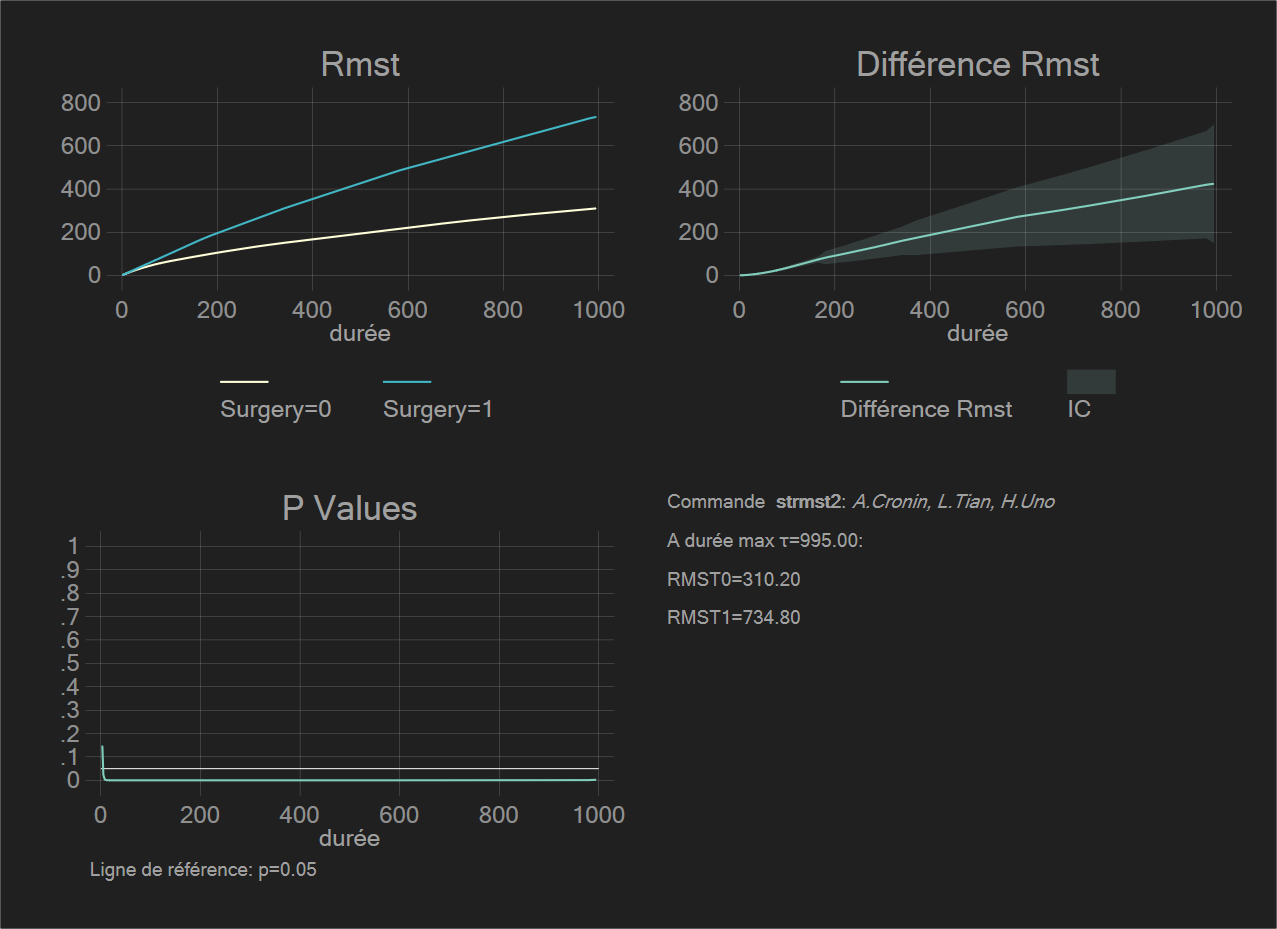
\includegraphics[width=0.7\textwidth,height=\textheight]{images/image9rmst.png}

}

\end{figure}

\part{Modèles à risques proportionnels}

\hypertarget{introduction-1}{%
\chapter{\texorpdfstring{\textbf{Introduction}}{Introduction}}\label{introduction-1}}

\hypertarget{proprortionalituxe9-des-risques}{%
\chapter{Proprortionalité des
risques}\label{proprortionalituxe9-des-risques}}

La spécification usuelle d'un modèle à risque proportionnel est:

\[h(t)=h_0(t)\times e^{X^{'}b}\]

\begin{itemize}
\item
  \(h(t)\) est une fonction de risque (ou taux de risque).
\item
  \(h_0(t)\) est une fonction qui dépend de la durée mais pas des
  caractéristiques individuelles. Il définiera le risque de base, et
  jouera donc le rôle de la constante dans un modèle classique.
\item
  \(e^{X^{'}b}\) est une fonction qui ne dépend pas de la durée, mais
  des caractéristiques individuelles \(X^{'}b=\sum_{k=1}^{p}b_kX_k\). La
  forme exponentielle assurera sa positivité \footnote{On rappelera
    qu'en durée continue, seule positivité du risque doit être assurée,
    d'où l'expression \emph{hazard rate}}.
\end{itemize}

\textbf{Le risque de base}

\textbf{\(h(t)=h_0(t)\)} donc \textbf{\(e^{X^{'}b}=1\)}. Observations
pour lesquelles \(X=0\)

\textbf{Risques proportionnels}

Cette hypothèse stipule l'invariance dans la durée du \emph{rapport des
risques} (\textbf{hazard ratio}).

Exemple:\\
Avec une seule covariable \(X\) introduite au modèle, et 2 observations
disons \(A\) et \(B\):

\begin{itemize}
\tightlist
\item
  \(h_A(t)=h_0(t)e^{bX_{A}}\)
\item
  \(h_B(t)=h_0(t)e^{bX_{B}}\).
\end{itemize}

Le rapport des risques entre \(A\) et \(B\) est simplement égal à:

\[\frac{h_A(t)}{h_B(t)}= \frac{e^{bX_A}}{e^{bX_B}}=e^{b(X_A-X_B)}\]

Autrement dit, cette proportionnalité des risques est la traduction
d'une absence d'interaction entre les rapports de risques estimés par un
modèle à risque proportionnel et la durée (ou une fonction de celle-ci).

\begin{figure}

\caption{L'hypothèse de proportionalite des risques}

{\centering 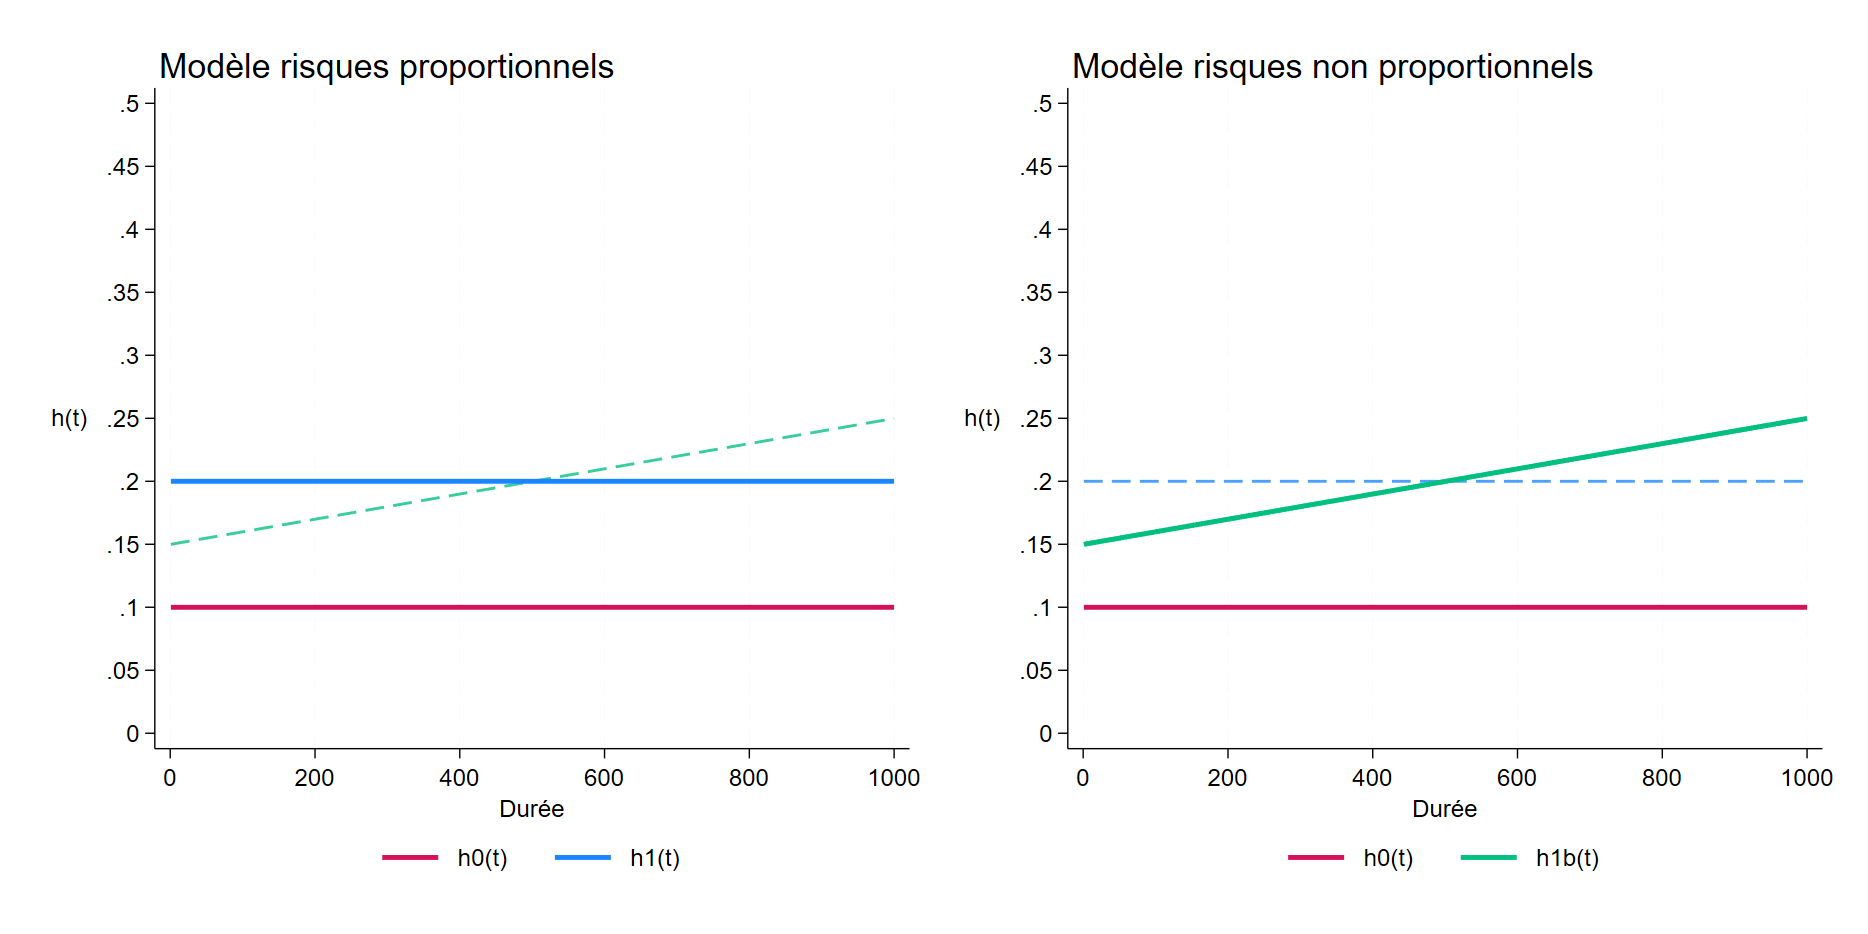
\includegraphics[width=0.7\textwidth,height=\textheight]{images/Image18.png}

}

\end{figure}

Si on part d'un modèle tel que \(h_0(t)=0.1\) quelque soit \(t\)
(baseline à risque constant).

Si \(h_1(t)\) est lui même constant, le rapport entre \(h_1(t)\) et
\(h_0(t)\) sera lui même constant dans la durée. On dit que les risques
sont proportionnels. Ici, \(h_1(t)=0.2\) quel que soit \(t\), le rapport
des risques est toujours égal à \(\frac{0.2}{0.1}=2=e^{b}\). Le
paramètre estimé par un modèle à risque proportionnel sera égal à
\(log(2)=0.69\).

Pour \(h_{1b}(t)\), le risque augmente de manière à un rythme constant
(linéaire): \(h_{1b}(1)=0.15\) et \(h_{1b}(1000)=0.25\). Comme
\(h_0(t)*\) est constant, le rapport des risques s'accroît également. On
dit que les risques ne sont pas proportionnels.

Si on est dans le deuxième cas de figure, un modèle à risque
proportionnel estimera un rapport toujours égal à 2. Il estimera un
\emph{rapport moyen} sur la période d'observation.

\hypertarget{les-moduxe8les}{%
\chapter{Les modèles}\label{les-moduxe8les}}

\begin{itemize}
\item
  \textbf{Modèle semi-paramétrique de Cox (1972)}\\
  Le modèle estime directement les \(b\) indépendamment de \(h_0(t)\).
  C'est pour cela qu'il est appelé modèle
  \textbf{\emph{semi-paramétrique de Cox}}. Les rapports de risque
  (\(e^{b}\)) seront utilisés dans un deuxième temps pour estimer la
  baseline \(h_0(t)\), qui peut s'avérer nécessaire pour calculer des
  fonctions de survie ajustées. Le respect de l'hypothèse de
  proportionnalité est donc importante et doit donc être analysée.
\item
  \textbf{\emph{Modèle à durée discrète}} Sa spécification diffère
  quelque peu de la présentation usuelle d'un modèle à risque
  proportionnel. Toutefois, il est régi par une hypothèse de
  proportionnalité. Le non respect de l'hypothèse est moins critique car
  la baseline du taux de risque est estimée simultanément aux autres
  paramètres. Il est comme son nom l'indique, particulièrement adapté au
  durées discrètes ou groupées. Avec une spécification logistique, les
  Odds vont sous certaines conditions (souvent respectée), se confondre
  avec des probabilités/risques. Lorsque le nombre de points
  d'observations (\(t\)) n'est pas trop faible, les résultats obtenus
  sont très proches de ceux issus directement d'un modèle de Cox. On
  peut souligné que ce modèle a été à l'origine proposé par Cox lui même
  à la fin des années 60.
\item
  \textbf{Les modèles paramétriques standards}\\
  Les modèles dits de Weibull, exponentiel, Gompertz ont une
  spécification sous hypothèse de risque proportionnel. Ils seront
  traités brièvement dans les compléments. Historiquement, le modèle de
  Cox est une réponse à une possible difficulté dans l'ajustement du
  risque par une loi de distribution du risque a priori.
\item
  \textbf{Modèle paramétrique de Parmar-Royston} (non traité)\\
  \(h_0(t)\), via le risque cumulé \(H(t)\), est estimé simultanément
  avec les rapports de risques en utilisant la méthode des \emph{splines
  cubiques}. Il est maintenant implémenté dans les logiciels standards
  (R, Stata, Sas). Les rapports de risque obtenus sont très proches de
  ceux estimés par le modèle classique de Cox. Il offre donc une
  alternative surement intéressante au Cox standard, et il s'est
  maintenant largement diffusé dans l'analyse des effets cliniques.
\item
  \textbf{Modèle à non proportionnalité}: on a bien évidemment les
  modèles paramétriques de type \emph{AFT} (Accelerated Failure Time),
  le peut-être très prometteur modèle à \emph{pseudo observations}
  d'Andersen (j'espère en faire une courte présentation rapidement après
  avoir évaluer son passage en durée discrète). Dans le champ du machine
  learning, il y a depuis son origine une version modèle de survie dans
  les \emph{forêts aléatoires}.
\end{itemize}

\hypertarget{le-moduxe8le-de-cox}{%
\chapter{\texorpdfstring{\textbf{Le modèle de
Cox}}{Le modèle de Cox}}\label{le-moduxe8le-de-cox}}

On peut ignorer la partie sur l'estimation du modèle. On retiendra tout
de même qu'il est déconseillé d'utiliser la méthode dite \emph{exacte}
pour la correction de la vraisemblance, qui ne peut matériellement
fonctionner qu'avec un nombre très limité d'évènements observés
simultanément. Ce qui est plutôt rare avec des données à durées
discrètes ou groupées, très fréquentes dans les sciences sociales.

\hypertarget{le-moduxe8le-semi-paramuxe9trique-de-cox}{%
\section{Le modèle semi-paramétrique de
Cox}\label{le-moduxe8le-semi-paramuxe9trique-de-cox}}

\hypertarget{la-vraisemblance-partielle-et-estimation-des-paramuxe8tres}{%
\subsection{La vraisemblance partielle et estimation des
paramètres}\label{la-vraisemblance-partielle-et-estimation-des-paramuxe8tres}}

On se situe dans une situation où la durée est mesurée sur une échelle
strictement continue. Il ne peut donc y avoir qu'un seul évènement
observé en \(t_i\) (idem pour la censure).

On peut représenter le processus aléatoire d'une analyse de survie en
présence de censure à droite, avec l'équation de vraisemblance suivante:

\[L_i=f(t_i)^{\delta_i}S(t_i)^{1-\delta_i}\]

\begin{itemize}
\tightlist
\item
  \(f(t_i)\) est la valeur de la fonction de densité en \(t_i\)
\item
  \(S(t_i)\) est la valeur de la fonction de survie en \(t_i\)
\item
  \(\delta_i=1\) si l'évènement est observé: \(L_i=f(t_i)\)
\item
  \(\delta_i=0\) si l'observation est censurée: \(L_i=S(t_i)\)
\end{itemize}

\textbf{Vraisemblance partielle de Cox}

Comme \(f(t_i)=h(t_i)\times S(t_i)\) \footnote{Se reporter à la
  définition des grandeurs dans la section \emph{Théorie}}, on obtient:
\(L_i=[h(t_i)S(t_i)]^{\delta_i}S(t_i)^{1-\delta_i} = h(t_i)^{\delta_i}S(t_i)\).

Pour \(i=1,2,.....,n\), la vraisemblance s'ecrit donc:
\(L_i=\prod_{i=1}^{n}h(t_i)^{\delta_i}S(t_i)\).

On peut réécrire cette vraisemblance en la multipliant et en la divisant
par: \(\sum_{j\in R_i}h(t_i)\), où \(j\in R_i\) est l'ensemble des
observations soumises au risque en \(t_i\).

\[L=\prod_{i=1}^{n}\left[h(t_i)\frac{\sum_{j\in R}h(t_i)}{\sum_{j\in R}h(t_i)}\right]^{\delta_i}S(t_i)= \prod_{i=1}^{n}\left[\frac{h(t_i)}{\sum_{j\in R_i}h(t_i)}\right]^{\delta_i}\sum_{j\in R_i}h(t_i)^{\delta_i}S(t_i)\]

La vraisemblance partielle retient seulement le premier terme de la
vraisemblance, soit:

\[PL=\prod_{i=1}^{n}\left[\frac{h(t_i)}{\sum_{j\in R}h(t_i)}\right]^{\delta_i}\]

Une fois remplacée la valeur de \(h(t_i)\) par son expression en tant
que modèle à risques proportionnels, la vraisemblance partielle ne
dépendra plus de la durée. \textbf{Mais elle va dépendre de l'ordre
d'arrivée des évènements, c'est à dire leur rang}.

\emph{Remarque}: pour les observations censurées(\(\delta_i=0\)),
\(PL=1\). Toutefois, ces censures à droite entrent dans l'expression
\(\sum_{j\in R}h(t_i)\) tant qu'elles sont soumises au risque.

En remplaçant donc \(h(t_i)\) par l'expression \(h_0(t)e^{X_i^{'}b}\):

\[PL=\prod_{i=1}^{n}\left[\frac{h_0(t)e^{X_{i}^{'}b}}{\sum_{j\in R_i}h_0(t)e^{X_{j}^{'}b}}\right]^{\delta_i} =\prod_{i=1}^{n}\left[\frac{e^{X_i^{'}b}}{\sum_{j\in R_i}e^{X_{j}^{'}b}}\right]^{\delta_i}\]

L'expression \(\frac{e^{Xb}}{\sum_{j\in R}e^{Xb}}\) est donc bien une
probabilité, et la vraisemblance partielle est donc bien un produit de
probabilités. Pour un individu ayant connu l'évènement, la contribution
à la vraisemblance partielle est \textbf{la probabilité que l'individu
observe l'évènement en \(t_i\) sachant qu'un évènement (et un seul)
s'est produit}.

\begin{itemize}
\item
  Si \(\delta_i = 0\): \(PL_i = 1\)
\item
  Si \(\delta_i = 1\):
  \(PL_i =\frac{e^{X_i^{'}b}}{\sum_{j\in R_i}e^{X_{j}^{'}b}}\)
\end{itemize}

\emph{Condition nécessaire: pas d'évènement simultané}: en présence
d'évènements mesurés simultanément, l'estimation de la vraisemblance
doit faire l'objet d'une correction.

\emph{Correction de la vraisemblance avec des évènements simultanés}:

\begin{itemize}
\item
  La \textbf{\emph{méthode dite exacte}}: Comme il ne doit pas y avoir
  d'évènement simultané, on va introduire à la vraisemblance partielle
  toutes les permutations possibles des évènements observés au même
  moment. Bien qu'en \(t_i\) on observe au même moment l'évènement pour
  2 observations (A,B) une métrique temporelle plus précise permettrait
  de savoir si A s'est produit avant B ou B s'est produit avant A (2
  permutations). Comme le nombre de permutations est calculé à l'aide
  d'une factorielle \footnote{\(n! = (n)\times(n-1)\times(n-2)\times....\times3\times2\times1\)},
  avec 3 évènements mesurés simultanément, on obtient 6 permutations
  (\(3\times2\times1\)). Problème: le nombre de permutations pour chaque
  \(t_i\) peut devenir très vite particulièrement élevé. Par exemple
  pour 10 évènements simultanés, le nombre de permutations est égal à
  3,628,800. Le temps de calcul devient extrêmement long, et ce type de
  correction totalement inopérant.
\item
  La \textbf{\emph{méthode dite de Breslow}}: il s'agit d'une
  approximation de la méthode exacte permettant de ne pas avoir à
  intégrer chaque permutation. \emph{Cette approximation est utilisée
  par défaut par les logiciels Sas et Stata}.
\item
  La \textbf{\emph{méthode dite d'Efron}}: elle corrige l'approximation
  de Breslow, et est jugée plus proche de la méthode exacte. \emph{C'est
  la méthode utilisée par défaut avec le logiciel R}, et elle est
  disponible avec les autres applications.
\end{itemize}

\hypertarget{estimation-des-paramuxe8tres}{%
\subsection{Estimation des
paramètres}\label{estimation-des-paramuxe8tres}}

On utilise la méthode habituelle, à savoir la maximisation de la
log-vraisemblance (ici partielle).

\begin{itemize}
\tightlist
\item
  Conditions de premier ordre: calcul des équations de score à partir
  des dérivées partielles. Solution:
  \(\frac{\partial log(PL)}{\partial{b_k}}=0\). On ne peut pas obtenir
  de solution numérique directe.
\end{itemize}

Remarque: les équations de score sont utilisées pour tester la validité
de l'hypothèse de constance des rapports de risque pour calculer les
\textbf{résidus de Schoenfeld} (voir plus loin).

\begin{itemize}
\item
  Conditions de second ordre: calcul des dérivées secondes qui
  permettent d'obtenir la matrice d'information de Fisher et la matrice
  des variances-covariances des paramètres.
\item
  Comme il n'y a pas de solution numérique directe, on utilise un
  algorithme d'optimisation (ex: Newton-Raphson) à partir des équations
  de score et de la matrice d'information de Fisher.
\end{itemize}

\textbf{Eléments de calcul}

En logarithme (sans évènement simultané), la vraisemblance partielle
s'ecrit:

\[pl(b)=\sum_{i=1}^n\delta_i\left(log(e^{X_{i}^{'}b})-log\sum_{j\in R_i}e^{X_{j}^{'}b}\right)\]

\[pl(b)=\sum_{i=1}^n\delta_i\left(X_{i}^{'}b-log\sum_{j\in R_i}e^{X_{j}^{'}b}\right)\]

Calcul de l'équation de score pour une covariable \(X_k\):

\[\frac{\partial pl(b)}{\partial{b_k}}=\sum_{i=1}^n\delta_i\left(X_{ik}-\sum_{j\in R_i}X_{jk}\frac{e^{X_{j}^{'}b}}{\sum_{j\in R_i}e^{X_{j}^{'}b}}\right)\]

Comme \(\frac{e^{X_{j}b}}{\sum_{j\in R}e^{X_{j}b}}\) est une
probabilité, et \(\sum_{j\in R}X_{ik}\times p_i\) est l'espérance (la
moyenne) \(E(X_k)\) d'avoir la caractéristique \(X_k\) lorsqu'un
évènement a été observé. Au final:

\[\frac{\partial lp(b)}{\partial{b_k}}= \sum_{i=1}^n\delta_i\left(X_{ik} - E(X_{j\in R_i,k}) \right)\]

Cette expression va permettre d'analyser le respect ou non de
l'hypothèse de risques proportionnels via les \emph{résidus de
Schoenfeld}.

\hypertarget{lecture-des-ruxe9sultats}{%
\subsection{Lecture des résultats}\label{lecture-des-ruxe9sultats}}

Comme il s'agit d'un modèle à risque proportionnel, \textbf{les rapports
de risques sont constants pendant toute la période d'observation}. Il
s'agit d'une \textbf{propriété de l'estimation}.

\textbf{\emph{Covariable binaire (indicatrice)}} \(X=(0,1)\):
\(RR=\frac{h(t\ |\ X=1)}{h(t\ |\ X=0)}=e^b\).\\
A chaque moment de la durée \(t\), le risque d'observer l'évènement est
\(e^b\) fois plus important/plus faible pour \(X=1\) que pour \(X=0\).

\textbf{\emph{Covariable quantitative}} (fixe dans le temps)

\(RR=\frac{h(t\ |\ X=a+c)}{h(t\ |\ X=a)}=e^{c \times{b}}\). On prendra
pour illustrer une variable type âge au début de l'exposition au risque
(a) et un delta de comparaison avec un âge inférieur c.\\
Si \(c=1\) (résultat de l'estimation): A un âge donnée, le risque de
connaitre l'évènement est \(e^b\) fois inférieur/supérieur à celui d'une
personne qui a un an de moins.

\textbf{Exemple pour les insuffisances cardiaques}

\begin{itemize}
\item
  Correction de la vraisemblance: méthode d'Efron
\item
  Nombre d'observations: 103
\item
  Nombre de décès: 75
\item
  Log-Vraisemblance: -289.30639
\end{itemize}

\begin{longtable}[]{@{}llllll@{}}
\caption{Cox: log Hazard Ratio (Risks Ratio)}\tabularnewline
\toprule\noalign{}
Variables & logRR & Std.Err & z & \(P>|z|\) & 95\% IC \\
\midrule\noalign{}
\endfirsthead
\toprule\noalign{}
Variables & logRR & Std.Err & z & \(P>|z|\) & 95\% IC \\
\midrule\noalign{}
\endhead
\bottomrule\noalign{}
\endlastfoot
year & -0.119 & 0.0673 & -1.78 & 0.076 & -0.2516;+0.0124 \\
age & +0.0296 & 0.0135 & 2.19 & 0.029 & +0.0031;+0.0561 \\
surgery & -0.9873 & 0.4363 & -2.26 & 0.024 & -1.8424;-0.1323 \\
\end{longtable}

\begin{longtable}[]{@{}llllll@{}}
\caption{Cox: Hazard Ratio (Risks Ratio)}\tabularnewline
\toprule\noalign{}
Variables & RR & Std.Err & z & \(P>|z|\) & 95\%CI \\
\midrule\noalign{}
\endfirsthead
\toprule\noalign{}
Variables & RR & Std.Err & z & \(P>|z|\) & 95\%CI \\
\midrule\noalign{}
\endhead
\bottomrule\noalign{}
\endlastfoot
year & 0.8872 & 0.0597 & -1.78 & 0.076 & 0.7775; 1.0124 \\
age & 1.0300 & 0.0139 & 2.19 & 0.029 & 1.0031; 1.0577 \\
surgery & 0.3726 & 0.1625 & -2.26 & 0.024 & 0.1584; 0.8761 \\
\end{longtable}

On retrouve les des tests non paramétriques pour l'opération, à savoir
qu'un pontage réduit les risques journaliers de décès pendant la période
d'observation (augmente la durée de survie).\\
De la même manière, plus on entre à un âge élevé dans la liste d'attente
plus le risque de décès augmente. La variable \emph{year}, qui traduit
des progrès en médecine, renvoie à une réduction plutôt modérée du
risque journalier de décès durant l'attente d'une greffe.

\textbf{R-Stata-Sas-Python}

\subsection{R}

Le modèle est estimé avec la fonction \textbf{\texttt{coxph}} de la
librairie \textbf{\texttt{survival}}. Hors options, la syntaxe est
identiques aux fonctions \texttt{survfit} et \texttt{survdif}.

\subsection{Stata}

Le modèle est estimé avec la commande \textbf{\texttt{stcox}}.

\subsection{SAS}

Le modèle est estimé avec la \textbf{\texttt{proc\ phreg}}.

\subsection{Python}

Avec la librairie \texttt{lifelines}, le modèle est estimé avec la
fonction \textbf{\texttt{CoxPHFitter}}. Avec la librairie
\texttt{statmodels}, il est estimé avec la fonction \texttt{smf.phreg}.

\hypertarget{analyse-de-la-constance-des-rapports-de-risque}{%
\section{Analyse de la constance des rapports de
risque}\label{analyse-de-la-constance-des-rapports-de-risque}}

\begin{itemize}
\item
  Les rapports de risque (RR) estimés par le modèle sont contraints à
  être constant sur toute la période d'observation. C'est une hypothèse
  forte.
\item
  Le respect de cette hypothèse doit être analysé, en particulier pour
  le modèle de Cox où la baseline du risque est habituellement estimée à
  l'aide de ces rapports (par exemple la méthode dite de Breslow, non
  traitée). En post-estimation, les valeurs estimées du risque pourront
  présenter des valeurs aberrantes si on dévie trop de constance, en
  particulier en obtenant des négatives des taux de risque.
\item
  Analyser cette hypothèse revient à introduire une interaction entre
  les rapports et la durée ou plutôt précisément une fonction de la
  durée).
\item
  Plusieurs méthodes disponibles, on traitera celles basées sur les
  \textbf{résidus de Schoenfeld}, et l'introduction directe d'une
  intéraction entre une fonction la durée et les covariables du modèle.
  Cette dernière fait également office de méthode de correction lorsque
  la violation de l'hypothèse est jugée trop importante ou problématique
  du point de vue des résultats obtenus.
\item
  Si on regarde les courbes de Kaplan-Meier, leurs croisement non tardif
  impliquera nécessairement un problème sur cette hypothèse.
\end{itemize}

\hypertarget{test-de-grambsch-therneau-sur-les-ruxe9sidus-de-schoenfeld}{%
\subsection{Test de Grambsch-Therneau sur les résidus de
Schoenfeld}\label{test-de-grambsch-therneau-sur-les-ruxe9sidus-de-schoenfeld}}

Ce test a été proposé par P.Grambsch et T.Therneau \footnote{Il s'agit
  bien de la personne qui maintient le package
  \textbf{\texttt{survival}} dans R} dans un cadre à durée strictement
continue. Il repose originellement sur une régression linéaire estimé
avec les moindres carrés généralisés (GLS) correction de
l'autocorrélation des erreurs avec des sér) . Dans un premier temps pour
des raisons plutôt pratiques (informatique), le test a une version
moindres carrés ordinaires (OLS). Jusqu'en 2020, tous les logiciels ne
proposaient que le test OLS. T.Therneau avec la V3 de package
\texttt{survival} a substitué - assez brutalement - le test GLS au test
OLS. Si les résultats sont proches dans le cadre d'une durée continue et
que le test GLS peut être considéré comme un test \emph{exact}, cela
devient problématique dans une situation de durée discrète/groupée
\footnote{Pour les personnes utilisant R, je donne un moyen pour
  récupérer et exécuter le test OLS sous R}. Le test OLS reste, à mon
sens, la méthode à privilégier dans le cas discret.

Il est également important de souligner que pour P.Grambsch et
T.Therneau \footnote{Se reporter à leur ouvrage \emph{Modeling Survival
  Data: Extending the Cox Model} (2001)} n'est qu'un moyen parmi
d'autres d'analyser une violation de l'hypothèse de proportionnalité. Ce
n'est pas \emph{the solution} (comme tout autre test au passage). Le
croisement des courbes de séjours peut-être suffisant pour alerter sur
cette violation.

\textbf{\emph{Principe du test}}: consiste à regarder la corrélation
entre les \textbf{résidus de Schoenfeld} obtenus directement avec la
fonction de score de la vraisemblanc partielle de Cox et une fonction de
la durée.

\textbf{\emph{Principe de calcul des résidus}}

\begin{itemize}
\tightlist
\item
  Les résidus \emph{bruts} sont directement calculés à partir des
  équations de scores {[}voir section estimation{]}.
\item
  Ils ne sont calculés que pour les observations qui ont connues
  l'évènement, au moment où un évènement s'est produit.
\item
  La somme des résidus pour chaque covariable est égale à 0. Il s'agit
  de la propriété de l'équation de score à l'équilibre.
\item
  On utilise généralement les \emph{résidus standardisés} (\emph{remis à
  l'échelle} / scaled) - par leur variance -. C'est la mesure de cette
  variance qui distingue le test OLS du test GLS.
\end{itemize}

Pour une observation dont l'évènement s'est produit en \(t_i\), le
\emph{résidu brut de Schoenfeld} pour la covariable \(X_k\), après
estimation du modèle, est égal à:

\[rs_{ik}=X_{ik}- \sum_{j\in R_i}X_{jk}\frac{e^{X_{j}^{'}b}}{\sum_{j\in R_i}e^{X_{j}^{'}b}}= X_{ik} - E(X_{j\in R_i})\]

\begin{itemize}
\item
  Ce résidu est formellement la contribution d'une observation ou d'un
  moment d'évènement au score. Il se lit comme la différence entre la
  valeur observée d'une covariable et sa valeur espérée au moment où
  l'évènement s'est produit.
\item
  Si la constance des rapports de risque varie peu les résidus ne
  doivent pas suivre une tendance précise localement ou globalement, à
  la hausse ou à la baisse.
\end{itemize}

Pourquoi?

Par l'exemple, sans censure à droite et en ne considérant que les
résidus bruts: Avec un rapport de risque strictement égal à 1 en début
d'exposition, une population soumise au risque \(R_i=100\) avec 50
hommes et 50 femmes. Si l'hypothèse PH (strictement) respectée,
lorsqu'il reste 90 personnes soumises au risque, on devrait avoir 45
hommes et 45 femmes. Avec \(R_i=50\), 25 hommes et 25
femmes,\ldots\ldots.avec \(R_i=10\), 5 hommes et 5 femmes.\\
Au final l'espérance d'avoir la caractéristique \(X\) est toujours égal
à 0.5 et les résidus bruts prendront toujours la valeur -.5 si \(X=0\)
et .5 si \(X=1\). En faisant une simple régression linéaire entre les
résidus, qui alternent ces deux valeurs, et \(t\), le coefficient estimé
sera en toute logique très proche de 0.

De manière encore plus simple, cette proportionnalité avec un risque
ratio égal à 1 suggère qu'au cours de la durée d'observation, on observe
une succession d'un même nombre d'hommes et de femmes qui connaissent
l'évènement. Si tous les hommes ou presque avaient observés l'évènement
plutôt en début d'éxposition et si toutes les femmes ou presque avaient
observé l'évènement plutôt en fin d'exposition, l'hypothèse de
proportionnalité pourraient fortement remise en cause.

On trouvera des éléments de calcul du test OLS
\href{https://mthevenin.github.io/analyse_duree/annexes/residusch.html}{ici}

\begin{tcolorbox}[enhanced jigsaw, arc=.35mm, bottomrule=.15mm, titlerule=0mm, colbacktitle=quarto-callout-warning-color!10!white, left=2mm, opacitybacktitle=0.6, toprule=.15mm, title=\textcolor{quarto-callout-warning-color}{\faExclamationTriangle}\hspace{0.5em}{Avertissement}, colframe=quarto-callout-warning-color-frame, breakable, coltitle=black, opacityback=0, toptitle=1mm, bottomtitle=1mm, rightrule=.15mm, leftrule=.75mm, colback=white]

\begin{itemize}
\item
  \textbf{Test omnibus}: Ne pas l'utiliser bien qu'il figure
  généralement en bas des output. Il n'a pas d'interprétation directe,
  et les p-value peuvent présenter des valeurs très faibles alors que ce
  n'est pas le cas pour les covariables prises une à une. Rester comme
  c'est souvent le cas à un test à un degré de liberté.
\item
  \textbf{Transformations de la durée}: n'importe quelle fonction de la
  durée peut être utilisée pour réaliser le test. On retient
  généralement les fonctions suivantes: \(g(t)=t\) (« identity »),
  \(g(t)=log(t)\), \(g(t)=KM(t)\) ou \(g(t)=1- S(t\)) où \(S(t\)) est
  l'estimateur de Kaplan-Meier. Enfin une transformation appelée « rank
  » est utilisée seulement pour les durées strictement continue ou
  suffisamment dispersées . Par exemple \(t=(0.1,0.5,1,2.6,3)\) donne
  une transformation \(t=(1,2,3,4)\). A savoir : \$g(t)=t rend le test
  relativement sensible aux évènements tardifs lorsque la population
  restant soumise est peu nombreuse (outliers).
\item
  Par défaut Stata, Sas, Python: \(g(t)=t\)
\item
  Par défaut R: \(g(t)= 1 - S(t)\)
\end{itemize}

\end{tcolorbox}

Pour des raisons de reproductibilité dans l'espace des logiciels et dans
le temps pour les différentes versions du package \texttt{survival} de
R, on ne présente ici que la version OLS.

\textbf{Test OLS avec \(g(t)=t\)}

\begin{longtable}[]{@{}llll@{}}
\caption{Test OLS Grambsch-Therneau avec \(g(t)=t\)}\tabularnewline
\toprule\noalign{}
Variables & chi2 & df & P\textgreater Chi2 \\
\midrule\noalign{}
\endfirsthead
\toprule\noalign{}
Variables & chi2 & df & P\textgreater Chi2 \\
\midrule\noalign{}
\endhead
\bottomrule\noalign{}
\endlastfoot
year & 0.80 & 1 & 0.3720 \\
age & 1.61 & 1 & 0.2043 \\
surgery & 5.54 & 1 & 0.0186 \\
\end{longtable}

Ici l'hypothèse de proportionnalité des risques est questionnable pour
la variable \emph{surgery}. Le risque ratio pourrait ne pas constant
dans le temps. Ce n'est pas du tout étonnant, le premier décès pour les
personnes opérées d'un pontage n'est observé qu'au bout de 165 jours. Au
final, un test était-il bien nécessaire pour arriver à ce constat
???????

\textbf{Test OLS avec \(g(t)=1- S(t)\)}

\begin{longtable}[]{@{}llll@{}}
\caption{Test Grambsch-Therneau avec \(g(t)=1- S(t)\)}\tabularnewline
\toprule\noalign{}
Variables & chi2 & df & P\textgreater Chi2 \\
\midrule\noalign{}
\endfirsthead
\toprule\noalign{}
Variables & chi2 & df & P\textgreater Chi2 \\
\midrule\noalign{}
\endhead
\bottomrule\noalign{}
\endlastfoot
year & 1.96 & 1 & 0.162 \\
age & 1.15 & 1 & 0.284 \\
surgery & 3.96 & 1 & 0.046 \\
\end{longtable}

\textbf{R-Stata-Sas-Python}

\subsection{R}

\textbf{\emph{Attention seulement version GLS du test depuis le V3 de
survival}}.

\begin{itemize}
\tightlist
\item
  Après avoir créer un objet à l'estimation du modèle de Cox, on utilise
  la fonction \textbf{\texttt{cox.zph}}. Cette fonction utilise par
  défaut \(g(t)=1-S(t)\) où \(S(t)\) sont les estimateurs de la courbe
  de Kaplan-Meier. On peut modifier cette fonction. Il est préférable de
  conserver cette fonction par défaut.
\item
  Test OLS: j'ai récupéré le programme du test antérieur, renommé
  \textbf{\texttt{cox.zphold}}. On peut le charger simplement, et il est
  facilement exécutable. Pour le charger:
  \texttt{source("https://raw.githubusercontent.com/mthevenin/analyse\_duree/main/cox.zphold/cox.zphold.R")}
\end{itemize}

\subsection{Stata}

Le test (OLS) est obtenu avec la commande
\textbf{\texttt{estat\ phtest,\ d}}. Par défaut Stata utilise
\(g(t)=t\). On peut modifier cette fonction.

\subsection{SAS}

Le test (OLS) est disponible depuis quelques années avec l'argument
\textbf{\texttt{zph}} sur la ligne \texttt{proc\ lifetest}. Par défaut
SAS utilise \(g(t)=t\). On peut modifier cette fonction.

\subsection{Python}

Le test (OLS) est donné avec la fonction
\textbf{\texttt{proportional\_hazard\_test}} de la librairie
\texttt{lifelines}. La fonction utilise par défaut \(g(t)=t\), mais on
peut afficher les résultats pour toutes les transformations de \(t\)
disponibles avec l'option \texttt{time\_transform=’all’}.

\hypertarget{intuxe9raction-avec-la-duruxe9e}{%
\subsection{Intéraction avec la
durée}\label{intuxe9raction-avec-la-duruxe9e}}

\textbf{\emph{Petit retour sur l'estimation du modèle}}

Pour estimer le modèle de Cox, les données sont dans un premier temps
splitées aux moment où au moins un évènement a été observé.

Sur l'application, avec 2 individus avec la covariable \emph{age}
(rappel: il s'agit de l'âge en \(t_0\):

\begin{longtable}[]{@{}lllll@{}}
\caption{Base spittées sur les intervals d'évènement}\tabularnewline
\toprule\noalign{}
id & age & died & \(t_0\) & \(t\) \\
\midrule\noalign{}
\endfirsthead
\toprule\noalign{}
id & age & died & \(t_0\) & \(t\) \\
\midrule\noalign{}
\endhead
\bottomrule\noalign{}
\endlastfoot
2 & 51 & 0 & 0 & 1 \\
2 & 51 & 0 & 1 & 2 \\
2 & 51 & 0 & 2 & 3 \\
2 & 51 & 0 & 3 & 5 \\
2 & 51 & 1 & 5 & 6 \\
3 & 54 & 0 & 0 & 1 \\
3 & 54 & 0 & 1 & 2 \\
3 & 54 & 0 & 2 & 3 \\
3 & 54 & 0 & 3 & 5 \\
3 & 54 & 0 & 5 & 6 \\
3 & 54 & 0 & 6 & 8 \\
3 & 54 & 0 & 8 & 9 \\
3 & 54 & 0 & 9 & 12 \\
3 & 54 & 1 & 12 & 16 \\
\end{longtable}

Les bornes des intervalles \([t_0;t]\) présentent des valeurs seulement
lorsqu'un évènement s'est produit (principe de la vraisemblance
partielle). Il n'y a donc pas de valeurs pour \(t\) et \(t_0\) en
\(t=4\) pour \(id=(2,3)\)et \(t=7,10,11,13,14,15\) pour \(id=3\).\\
Les deux individus observent l'évènement en \(t=6\) pour \(id=2\), et en
\(t=16\) pour \(id=3\). Avant ce moment la valeur de la variable
évènement/censure (ici \(d\)) prend toujours la valeur 0, et prend la
valeur 1 le jour du décès.

Sur cette base \emph{splitée} aux moments d'évènement (n=3573), on
pourra vérifier facilement que les résultats obtenus par le modèle de
Cox sont identiques à ceux obtenus précédemment.

\emph{Introduction d'une intéraction avec une fonction de la durée}

On a une variable de durée (on prendra \(g(t)=t\)) qui sera croisée avec
la variable \emph{surgery}.

Le modèle s'écrit:

\[h(t | X,t) = h_0(t)e^{b_1age + b_2year + b_3 surgery + b_4 (surgery\times t)}\]

Le modèle avec cette intéraction donne les résultats suivants:

\begin{longtable}[]{@{}
  >{\raggedright\arraybackslash}p{(\columnwidth - 10\tabcolsep) * \real{0.2836}}
  >{\raggedright\arraybackslash}p{(\columnwidth - 10\tabcolsep) * \real{0.1045}}
  >{\raggedright\arraybackslash}p{(\columnwidth - 10\tabcolsep) * \real{0.1343}}
  >{\raggedright\arraybackslash}p{(\columnwidth - 10\tabcolsep) * \real{0.1045}}
  >{\raggedright\arraybackslash}p{(\columnwidth - 10\tabcolsep) * \real{0.1493}}
  >{\raggedright\arraybackslash}p{(\columnwidth - 10\tabcolsep) * \real{0.2239}}@{}}
\caption{Modèle de Cox avec une intéraction entre une fonction de la
durée et la variable *surgery}\tabularnewline
\toprule\noalign{}
\begin{minipage}[b]{\linewidth}\raggedright
Variable
\end{minipage} & \begin{minipage}[b]{\linewidth}\raggedright
\(e^b\)
\end{minipage} & \begin{minipage}[b]{\linewidth}\raggedright
Std.err
\end{minipage} & \begin{minipage}[b]{\linewidth}\raggedright
z
\end{minipage} & \begin{minipage}[b]{\linewidth}\raggedright
P\textgreater\textbar z\textbar{}
\end{minipage} & \begin{minipage}[b]{\linewidth}\raggedright
95\% IC
\end{minipage} \\
\midrule\noalign{}
\endfirsthead
\toprule\noalign{}
\begin{minipage}[b]{\linewidth}\raggedright
Variable
\end{minipage} & \begin{minipage}[b]{\linewidth}\raggedright
\(e^b\)
\end{minipage} & \begin{minipage}[b]{\linewidth}\raggedright
Std.err
\end{minipage} & \begin{minipage}[b]{\linewidth}\raggedright
z
\end{minipage} & \begin{minipage}[b]{\linewidth}\raggedright
P\textgreater\textbar z\textbar{}
\end{minipage} & \begin{minipage}[b]{\linewidth}\raggedright
95\% IC
\end{minipage} \\
\midrule\noalign{}
\endhead
\bottomrule\noalign{}
\endlastfoot
year & 0.884 & 0.059 & -1.84 & 0.066 & 0.776 ; 1.008 \\
age & 1.029 & 0.014 & +2.15 & 0.032 & 1.003 ; 1.057 \\
\(surgery(t_{0+})\) & 0.173 & 0.117 & -2.60 & 0.009 & 0.046 ; 0.649 \\
\(surgery\times t\) & 1.002 & 0.001 & +2.02 & 0.043 & 1.000 ; 1.004 \\
\end{longtable}

On retrouve donc un résultat proche de celui obtenu à partir du test OLS
sur les résidus de Schoenfeld pour la variable \emph{surgery}. Et c'est
normal. Avec \(g(t)=t\), il a le mérite de pouvoir être interprété
directement. Ce qui ne veut pas dire qu'il s'agit de la meilleure
solution.

Donc, malgré une hypothèse plutôt forte sur la forme fonctionnelle de
l'intéraction, et dans les faits surement pas pertinente, on peut dire
que chaque jour le rapport des risques entre personnes opérées et
personnes non opérées augmente de +0.2\%. Pour plus précis, étant à
l'origine \textless1, l'écart se modère. L'effet de l'opération sur la
survie des individus s'estompe donc avec le temps.

\textbf{A noter}

\begin{itemize}
\tightlist
\item
  Le modèle n'est plus un modèle à risque proportionnel. La variable
  \emph{surgery} n'est plus une variable \textbf{fixe} mais une variable
  tronquée dynamique qui prend la valeur de \(t\) pour les personnes qui
  ont été opérées d'un pontage avant leur entrée dans le registre de
  greffe.
\end{itemize}

Si \(surgery = 0\)

\begin{longtable}[]{@{}llllll@{}}
\toprule\noalign{}
id & surgery & died & \(t_0\) & \(t\) & surgery*t \\
\midrule\noalign{}
\endhead
\bottomrule\noalign{}
\endlastfoot
2 & 0 & 0 & 0 & 1 & 0 \\
2 & 0 & 0 & 1 & 2 & 0 \\
2 & 0 & 0 & 2 & 3 & 0 \\
2 & 0 & 0 & 3 & 5 & 0 \\
2 & 0 & 1 & 5 & 6 & 0 \\
\end{longtable}

Si \(surgery = 1\) (jusqu'à \(t=6\) car aucun décès précoce pour ce
groupe)

\begin{longtable}[]{@{}llllll@{}}
\toprule\noalign{}
id & surgery & died & \(t_0\) & \(t\) & surgery*t \\
\midrule\noalign{}
\endhead
\bottomrule\noalign{}
\endlastfoot
40 & 1 & 0 & 0 & 1 & 1 \\
40 & 1 & 0 & 1 & 2 & 2 \\
40 & 1 & 0 & 2 & 3 & 3 \\
40 & 1 & 0 & 3 & 5 & 5 \\
40 & 1 & 1 & 5 & 6 & 6 \\
\end{longtable}

Exemple pour une variable quantitative (\emph{age})

\begin{longtable}[]{@{}llllll@{}}
\toprule\noalign{}
id & age & died & \(t_0\) & \(t\) & age*t \\
\midrule\noalign{}
\endhead
\bottomrule\noalign{}
\endlastfoot
2 & 51 & 0 & 0 & 1 & 51 \\
2 & 51 & 0 & 1 & 2 & 102 \\
2 & 51 & 0 & 2 & 3 & 153 \\
2 & 51 & 0 & 3 & 5 & 255 \\
2 & 51 & 1 & 5 & 6 & 306 \\
\end{longtable}

\begin{itemize}
\tightlist
\item
  L'altération des rapports de risque dépend de la forme fonctionnelle
  de l'intéraction choisie. Ici la variation dans la durée du rapport
  des risque est constante, ce qui est une hypothèse assez forte. On a,
  en quelques sorte, réintroduit une hypothèse de proportionnalité, ici
  sur le degré d'altération des écarts de risques dans le temps, qui
  devient lui même strictement constant.
\end{itemize}

\hypertarget{que-faire}{%
\subsection{Que faire ?}\label{que-faire}}

\textbf{\emph{Ne rien faire}}

On interprète le risque ratio comme un ratio moyen pendant la durée
d'observation (P.Allison). Difficilement soutenable pour l'analyse des
effets cliniques, elle peut être envisagée dans d'autres domaines.
Attention au nombre de variables qui ne respectent pas l'hypothèse,
l'estimation de la baseline du risque pourrait être sensiblement
affectée si l'analyse a des visée prédictives. Il convient tout de même
lors de l'interprétation, de préciser les variables qui seront analysées
sous cette forme très « moyenne » sur la période d'observation.

On peut également adapter cette stratégie du « ne rien faire » selon
sens de l'altération des rapports de risque. Si aux cours du temps des
écarts de risque, s'accentuent à la hausse comme à la baisse, on peut
conserver cet estimateur moyen. Mais si cette non proportionnalité
conduit à un changement du sens des rapport de risque je suis moins
convaincu de la pertinence de cette stratégie. Encore une fois, et il
faut le rappeler, l'estimation des courbes de survie doit permette
d'anticiper ce dernier cas de figure.

Il faut également tenir compte de l'intérêt portée par les variables qui
présentent un problème par rapport à l'hypothèse. Il n'est peut-être pas
nécessaire de complexifier le modèle pour des variables introduites
comme simples contrôles.

Mais plus problématique {[}\textbf{important}{]}\ldots{} On sait qu'une
des causes du non respect de l'hypothèse peut provenir d'effets de
sélection liées à des variables omises ou non observables. En analyse de
durée ce problème prend le nom de \textbf{\emph{frailty}} (fragilité)
lorsque cette non homogénéité n'est pas observable. Des estimations,
plus complexes, sont possibles dans ce cas, et sont en mesure malgré
leur interprétation plutôt difficile de régler le problème. Il convient
donc de bien spécifier le modèle au niveau des variables de contrôle
observables et disponibles.

\textbf{\emph{Modèle de Cox stratifié}}

Utiliser la méthode dite de « Cox stratifiée » (non traitée). Utile si
l'objectif est de présenter des fonctions de survie prédites ajustées,
et si une seule covariable (binaire) présente un problème. Les HR ne
seront pas estimés pour la variable qui ne respecte pas l'hypothèse.

\textbf{\emph{Intéraction}}

Introduire une interaction avec la durée. Cela peut permettre en plus
d'enrichir le modèle au niveau de l'interprétation. Valable si peu de
covariables présentent des problèmes de stabilité des rapports de
risque, dans l'idéal une seule variable. Attention tout de même à la
forme de la fonction, dans l'exemple on a contraint l'effet
d'interaction à être strictement linéaire, ce qui est une hypothèse
plutôt forte\ldots. on introduit de nouveau une contrainte de
proportionnalité dans le modèle.

\textbf{\emph{Modèles alternatifs}}

Utiliser un modèle alternatif: modèles paramétriques à risques
proportionnels si la distribution du risque s'ajuste bien, le modèle
paramétrique « flexible » de Parmar-Royston ou un modèle à temps
discret. Pour la dernière solution, on peut également corriger la non
proportionnalité avec l'introduction d'une intéraction. Si on ne le fait
pas, les risques prédits, par définition des probabilités
conditionnelles, resteront toujours dans les bornes contrairement au
modèle de Cox.\\
Utiliser un modèle non paramétrique additif dit d'Aalen ou une de ses
variantes (non traité). Mais ces modèles, dont les résultats sont
présentés par des graphiques, se commentent assez difficilement.

\textbf{Forêt aléatoire}\\
Autre méthode : les forêts aléatoires. L.Breiman a dès le départ proposé
une estimation des modèles de survie par cette méthode. Par définition,
pas sensible à l'hypothèse PH. Mais cela reste des méthodes à finalité
prédictive, moins riche en interprétation.

\hypertarget{moduxe8le-uxe0-duruxe9e-discruxe8te}{%
\chapter{\texorpdfstring{\textbf{Modèle à durée
discrète}}{Modèle à durée discrète}}\label{moduxe8le-uxe0-duruxe9e-discruxe8te}}

On va principalement traiter du \textbf{\emph{modèle logistique à durée
discrète}}.

\begin{itemize}
\tightlist
\item
  Par définition ce n'est pas un modèle à risques proportionnels, mais à
  \textbf{Odds proportionnels}. Toutefois en situation de rareté
  (p\textless10\%), l'Odds converge vers une probabilité, qui est une
  mesure du risque.
\item
  Le modèle à durée discrète est de type pleinement paramétrique, il est
  moins contraignant que le modèle de Cox si l'hypothèse de
  proportionnalité n'est pas respectée, car le modèle est ajusté par une
  fonction de la durée.
\item
  Pour être estimé, la base de données doit être transformée en format
  long: aux durées d'observation ou sur des intervalles de durée
  choisis. C'est une des principales différences avec le modèle de Cox
  qui est une estimation aux moments d'évènement. Néanmoins avec une
  bonne forme fonctionnelle de la durée traitée comme une variable
  quantitative, et si le nombre de points d'observation est suffisamment
  grand, les deux modèles aboutissent à des résultats quasiment
  identiques.
\item
  Ce modèle permet d'introduire de manière plutôt souple un ensemble de
  covariables no fixes.
\end{itemize}

Avec un lien logistique, le modèle à durée discrète, avec seulement des
covariables fixes, peut s'écrire:

\[log\left[\frac{P(Y=1\ |\ t_p,X_k)}{1-P(Y=1\ |\ t_p,X_k)}\right]= a_0 + \sum_{p}a_pf(t_p)+\sum_{k}b_kX_k\]

\hypertarget{organisation-des-donnuxe9es}{%
\section{Organisation des données}\label{organisation-des-donnuxe9es}}

\textbf{Format long}

Les données doivent être en format long: pour chaque individu on a une
ligne par durée observée ou par intevalle de durées jusqu'à l'évènement
ou la censure. On retrouve le \emph{split} des données du modèle de Cox,
mais généralisé à des intervalles où aucun évènement n'est observé. Avec
des données de type discrètes ou groupées, phénomène classique en
sciences sociales, il y a souvent peu de différence entre un allongement
aux temps d'évènement et aux temps d'observation.\\

\textbf{Durée}

La durée est dans un premier temps construite sous forme d'un simple
compteur, par exemple \(t=1,2,3,4,5...\) (des valeurs non entières sont
possibles). Le choix de la forme fonctionnelle de la durée sera
présentée plus tard.

\textbf{Variable évènement/censure}

Si l'individu a connu l'évènement, elle prend la valeur 0 avant
celui-ci. Au moment de l'évènement sa valeur est égale à 1. Pour les
observations censurées, la variable prend toujours la valeur 0.

\textbf{Application}\\
On reprend les données de la base \emph{transplantation}, mais les
durées ont été regroupées par période de 30 jours. Il n'y a pas de durée
mesurée comme nulle, on a considéré que les 30 premiers jours
représentaient, le premier mois d'exposition. Cette variable de durée se
nomme \emph{mois}.

\textbf{Format d'origine}

\begin{longtable}[]{@{}llllll@{}}
\caption{Durée discrète: données en format d'origine}\tabularnewline
\toprule\noalign{}
id & year & age & surgery & mois & died \\
\midrule\noalign{}
\endfirsthead
\toprule\noalign{}
id & year & age & surgery & mois & died \\
\midrule\noalign{}
\endhead
\bottomrule\noalign{}
\endlastfoot
1 & 67 & 30 & 0 & 2 & 1 \\
\end{longtable}

La personne décède lors du deuxième intervalle de 30 jours

\textbf{Format long et variables pour l'analyse}

\begin{longtable}[]{@{}lllllll@{}}
\caption{Durée discrète: données en format long}\tabularnewline
\toprule\noalign{}
id & year & age & surgery & mois & died & t \\
\midrule\noalign{}
\endfirsthead
\toprule\noalign{}
id & year & age & surgery & mois & died & t \\
\midrule\noalign{}
\endhead
\bottomrule\noalign{}
\endlastfoot
1 & 67 & 30 & 0 & 2 & 0 & 1 \\
1 & 67 & 30 & 0 & 2 & 1 & 2 \\
\end{longtable}

\hypertarget{ajustement-de-la-duruxe9e}{%
\section{Ajustement de la durée}\label{ajustement-de-la-duruxe9e}}

Un des principaux enjeux réside dans la paramétrisation de la durée:

\begin{itemize}
\tightlist
\item
  Elle peut-être modélisée sous forme de fonction d'une variable de type
  quantitative/continue.
\item
  Elle peut-être modélisée comme variable discrète, de type indicatrice
  \({0;1}\), sur tous les points d'observation, ou sous forme de
  regroupements. Il doit y avoir au moins un évènement observé dans
  chaque intervalle.
\end{itemize}

\hypertarget{ajustement-avec-une-duruxe9e-en-continu}{%
\subsection{Ajustement avec une durée en
continu}\label{ajustement-avec-une-duruxe9e-en-continu}}

Le modèle étant paramétrique, on doit trouver une fonction qui ajuste le
mieux les données. Toutes transformations de la variable est possible:
\(f(t)=a\times t\), \(f(t)=a\times ln(t)\)\ldots\ldots formes
quadratiques. Les ajustements sous forme de \textbf{splines} (cubiques)
tendent à se développer ces dernières années.

Pour sélectionner cette fonction, on peut tester différents modèles sans
covariable additionnelle, et sélectionner la forme dont le critère
d'information de type \textbf{AIC} (vraisemblance pénalisée) est le plus
faible.

Exemple:\\
On va tester les paramétrisations suivante:s une forme linéraire stricte
\(f(t)=a\times t\) et des effets quadratiques d'ordres 2 et 3:
\(f(t)=a_1\times t + a_2\times t^{2}\) et
\(f(t)=a_1\times t + a_2\times t^{2} + a_3\times t^{3}\).

\begin{figure}

\caption{Probabilité de décéder avec 3 ajustements de la durée}

{\centering 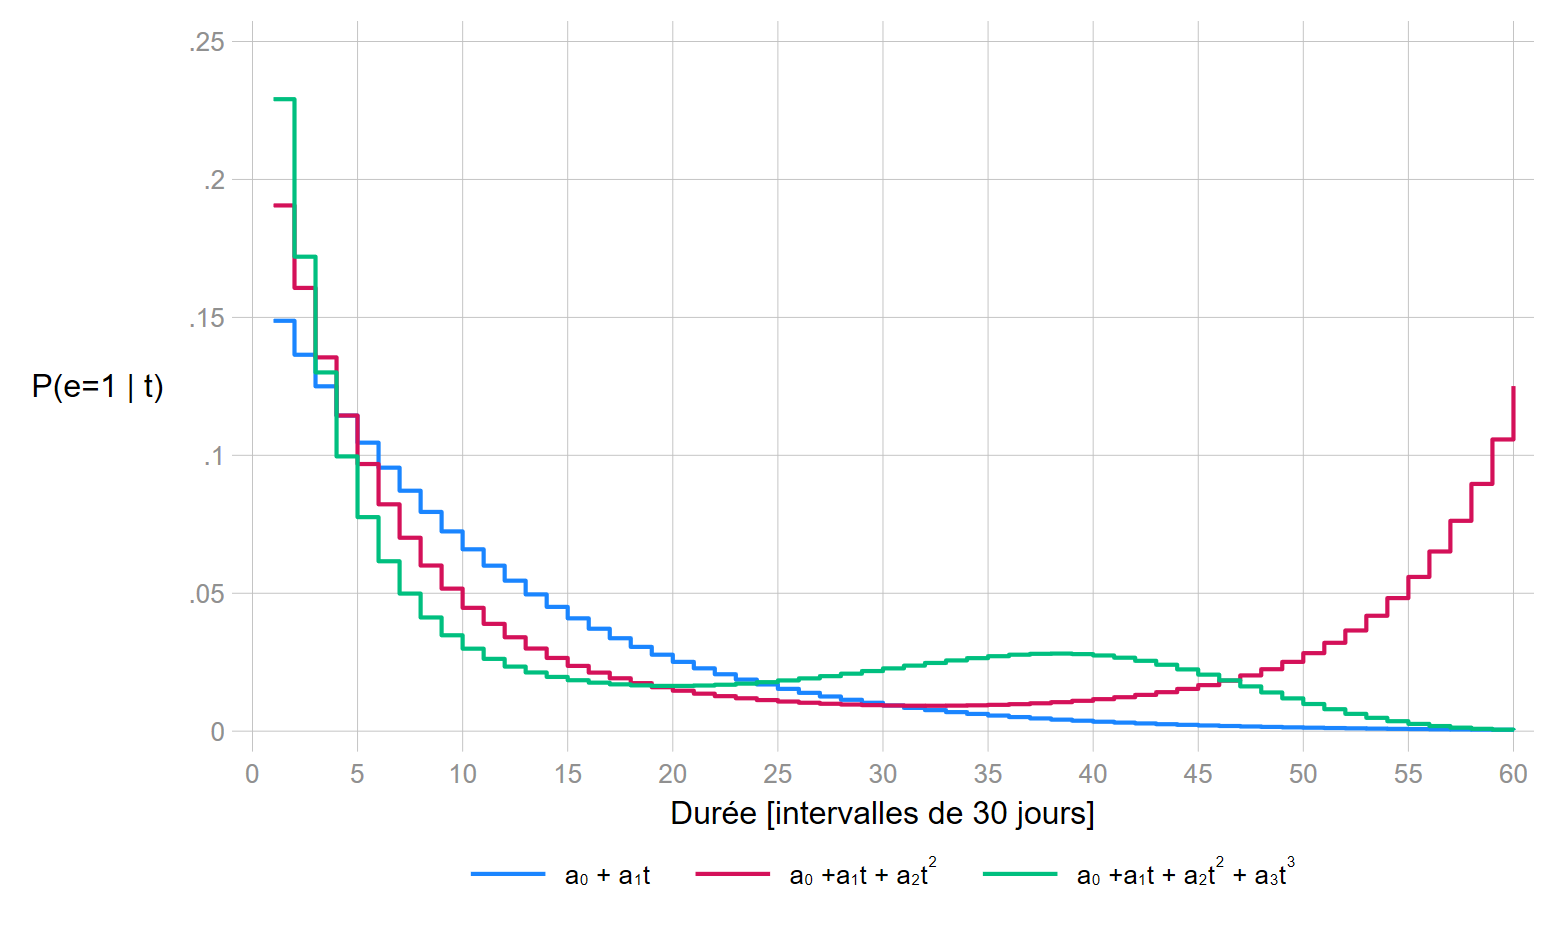
\includegraphics[width=0.7\textwidth,height=\textheight]{images/Image11.png}

}

\end{figure}

\textbf{Critères AIC}

\begin{longtable}[]{@{}ll@{}}
\toprule\noalign{}
\(f(t)\) & AIC \\
\midrule\noalign{}
\endhead
\bottomrule\noalign{}
\endlastfoot
\(a\times t\) & 504 \\
\(a_1\times t + a_2\times t^{2}\) & 492 \\
\(a_1\times t + a_2\times t^{2} + a_3\times t^{3}\) & 486 \\
\end{longtable}

On peut utiliser la troisième forme à savoir
\(a_1\times t + a_2\times t^{2} + a_3\times t^{3}\).

\textbf{Estimation du modèle avec toutes les covariables}

\begin{longtable}[]{@{}
  >{\raggedright\arraybackslash}p{(\columnwidth - 10\tabcolsep) * \real{0.1912}}
  >{\raggedright\arraybackslash}p{(\columnwidth - 10\tabcolsep) * \real{0.1324}}
  >{\raggedright\arraybackslash}p{(\columnwidth - 10\tabcolsep) * \real{0.1471}}
  >{\raggedright\arraybackslash}p{(\columnwidth - 10\tabcolsep) * \real{0.1324}}
  >{\raggedright\arraybackslash}p{(\columnwidth - 10\tabcolsep) * \real{0.1471}}
  >{\raggedright\arraybackslash}p{(\columnwidth - 10\tabcolsep) * \real{0.2500}}@{}}
\caption{Modèle logistique à durée discrète (\(f(t)\)
continue)}\tabularnewline
\toprule\noalign{}
\begin{minipage}[b]{\linewidth}\raggedright
Variables
\end{minipage} & \begin{minipage}[b]{\linewidth}\raggedright
OR - RR
\end{minipage} & \begin{minipage}[b]{\linewidth}\raggedright
Std. err
\end{minipage} & \begin{minipage}[b]{\linewidth}\raggedright
z
\end{minipage} & \begin{minipage}[b]{\linewidth}\raggedright
P\textgreater\textbar z\textbar{}
\end{minipage} & \begin{minipage}[b]{\linewidth}\raggedright
95\% IC
\end{minipage} \\
\midrule\noalign{}
\endfirsthead
\toprule\noalign{}
\begin{minipage}[b]{\linewidth}\raggedright
Variables
\end{minipage} & \begin{minipage}[b]{\linewidth}\raggedright
OR - RR
\end{minipage} & \begin{minipage}[b]{\linewidth}\raggedright
Std. err
\end{minipage} & \begin{minipage}[b]{\linewidth}\raggedright
z
\end{minipage} & \begin{minipage}[b]{\linewidth}\raggedright
P\textgreater\textbar z\textbar{}
\end{minipage} & \begin{minipage}[b]{\linewidth}\raggedright
95\% IC
\end{minipage} \\
\midrule\noalign{}
\endhead
\bottomrule\noalign{}
\endlastfoot
\(t\) & 0.678 & 0.057 & -4.52 & 0.000 & 0.587 ; 0.810 \\
\(t^2\) & 1.014 & 0.005 & +2.83 & 0.005 & 1.004 ; 1.024 \\
\(t^3\) & 1.000 & 0.000 & -2.11 & 0.035 & 1.000 ; 1.000 \\
\(year\) & 0.876 & 0.015 & -1.80 & 0.072 & 0.758 ; 1.012 \\
\(age\) & 1.034 & 0.163 & +2.27 & 0.023 & 1.005 ; 1.064 \\
\(surgery\) & 0.364 & 0.110 & -2.25 & 0.024 & 0.151 ; 0.877 \\
& & & & & \\
\emph{Constante} & \emph{0.440} & \emph{0.110} & \emph{-3.29} &
\emph{0.001} & \emph{0.270 ; 0.718} \\
\end{longtable}

\emph{Remarque}: les variables \emph{year} et \emph{age} ont été centrée
sur leur moyenne pour rendre la constante interprétable. La constante
reporte donc l'Odds de décéder lors des 30 premiers jours d'une personne
dont l'âge et l'année à l'entrée dans le registre est égal à l'âge et à
l'année moyenne et qui n'a pas été opéré préalablement.

Si maintenant on estime un modèle de Cox sur ces données journalières
groupées, on remarque que les résultats obtenus sont très proches

\begin{longtable}[]{@{}
  >{\raggedright\arraybackslash}p{(\columnwidth - 10\tabcolsep) * \real{0.1912}}
  >{\raggedright\arraybackslash}p{(\columnwidth - 10\tabcolsep) * \real{0.1324}}
  >{\raggedright\arraybackslash}p{(\columnwidth - 10\tabcolsep) * \real{0.1471}}
  >{\raggedright\arraybackslash}p{(\columnwidth - 10\tabcolsep) * \real{0.1324}}
  >{\raggedright\arraybackslash}p{(\columnwidth - 10\tabcolsep) * \real{0.1471}}
  >{\raggedright\arraybackslash}p{(\columnwidth - 10\tabcolsep) * \real{0.2500}}@{}}
\caption{Modèle de Cox}\tabularnewline
\toprule\noalign{}
\begin{minipage}[b]{\linewidth}\raggedright
Variables
\end{minipage} & \begin{minipage}[b]{\linewidth}\raggedright
OR - RR
\end{minipage} & \begin{minipage}[b]{\linewidth}\raggedright
Std. err
\end{minipage} & \begin{minipage}[b]{\linewidth}\raggedright
z
\end{minipage} & \begin{minipage}[b]{\linewidth}\raggedright
P\textgreater\textbar z\textbar{}
\end{minipage} & \begin{minipage}[b]{\linewidth}\raggedright
95\% IC
\end{minipage} \\
\midrule\noalign{}
\endfirsthead
\toprule\noalign{}
\begin{minipage}[b]{\linewidth}\raggedright
Variables
\end{minipage} & \begin{minipage}[b]{\linewidth}\raggedright
OR - RR
\end{minipage} & \begin{minipage}[b]{\linewidth}\raggedright
Std. err
\end{minipage} & \begin{minipage}[b]{\linewidth}\raggedright
z
\end{minipage} & \begin{minipage}[b]{\linewidth}\raggedright
P\textgreater\textbar z\textbar{}
\end{minipage} & \begin{minipage}[b]{\linewidth}\raggedright
95\% IC
\end{minipage} \\
\midrule\noalign{}
\endhead
\bottomrule\noalign{}
\endlastfoot
\(year\) & 0.878 & 0.059 & -1.93 & 0.053 & 0.769 ; 1.002 \\
\(age\) & 1.029 & 0.014 & +2.13 & 0.033 & 1.002 ; 1.057 \\
\(surgery\) & 0.379 & 0.165 & -2.22 & 0.026 & 0.111 ; 0.892 \\
\end{longtable}

\hypertarget{ajustement-discret}{%
\subsection{Ajustement discret}\label{ajustement-discret}}

\begin{itemize}
\tightlist
\item
  Il s'agit d'introduire la variable de durée dans le modèle comme une
  variable catégorielle (indicatrices).
\item
  Démarche pas conseillé si on a beaucoup de points d'observation, ce
  qui est le cas ici.
\item
  A l'inverse, si peu de points d'observation la paramétrisation avec
  une durée continue n'est pas conseillé.
\item
  La correction de la non proportionnalité peut être plus compliquée à
  mettre en oeuvre.
\end{itemize}

On va supposer que l'on ne dispose que de 4 intervalles d'observation.
Pour l'exemple, on va créer ces points à partir des quartiles de la
durée, et conserver pour chaque personne une seule observation par
intervalle.

\begin{itemize}
\tightlist
\item
  \(t=1\): Entre le début de l'exposition et 4 mois.
\item
  \(t=2\): Entre 5 mois et 11 mois .
\item
  \(t=3\): Entre 12 mois et 23 mois.
\item
  \(t=4\): 24 mois et plus.
\end{itemize}

On va estimer le risque globalement sur l'intervalle. La base sera plus
courte que la précédente (197 observations pour 103 individus). Il ne
sera plus possible ici d'interpréter les résultats en termes de rapport
de probabilité, l'évènement devenant trop fréquent à l'intérieur de
chaque intervalle.

\begin{longtable}[]{@{}
  >{\raggedright\arraybackslash}p{(\columnwidth - 10\tabcolsep) * \real{0.1912}}
  >{\raggedright\arraybackslash}p{(\columnwidth - 10\tabcolsep) * \real{0.1324}}
  >{\raggedright\arraybackslash}p{(\columnwidth - 10\tabcolsep) * \real{0.1471}}
  >{\raggedright\arraybackslash}p{(\columnwidth - 10\tabcolsep) * \real{0.1324}}
  >{\raggedright\arraybackslash}p{(\columnwidth - 10\tabcolsep) * \real{0.1471}}
  >{\raggedright\arraybackslash}p{(\columnwidth - 10\tabcolsep) * \real{0.2500}}@{}}
\caption{Modèle logistique à durée discrète (\(f(t)\)
indicatrices)}\tabularnewline
\toprule\noalign{}
\begin{minipage}[b]{\linewidth}\raggedright
Variables
\end{minipage} & \begin{minipage}[b]{\linewidth}\raggedright
OR - RR
\end{minipage} & \begin{minipage}[b]{\linewidth}\raggedright
Std. err
\end{minipage} & \begin{minipage}[b]{\linewidth}\raggedright
z
\end{minipage} & \begin{minipage}[b]{\linewidth}\raggedright
P\textgreater\textbar z\textbar{}
\end{minipage} & \begin{minipage}[b]{\linewidth}\raggedright
95\% IC
\end{minipage} \\
\midrule\noalign{}
\endfirsthead
\toprule\noalign{}
\begin{minipage}[b]{\linewidth}\raggedright
Variables
\end{minipage} & \begin{minipage}[b]{\linewidth}\raggedright
OR - RR
\end{minipage} & \begin{minipage}[b]{\linewidth}\raggedright
Std. err
\end{minipage} & \begin{minipage}[b]{\linewidth}\raggedright
z
\end{minipage} & \begin{minipage}[b]{\linewidth}\raggedright
P\textgreater\textbar z\textbar{}
\end{minipage} & \begin{minipage}[b]{\linewidth}\raggedright
95\% IC
\end{minipage} \\
\midrule\noalign{}
\endhead
\bottomrule\noalign{}
\endlastfoot
\(0-4 mois\) & 2.811 & 1.177 & +2.47 & 0.014 & 1.237 ; 6.387 \\
\(5-11 mois\) & ref & - & - & - & - \\
\(12-23 mois\) & 0.559 & 0.346 & -0.94 & 0.347 & 0.166 ; 1.881 \\
\(24-46 mois\) & 1.741 & 1.159 & +0.83 & 0.405 & 0.472 ; 6.417 \\
\(year\) & 0.816 & 0.076 & -2.18 & 0.029 & 0.680 ; 0.980 \\
\(age\) & 1.048 & 0.019 & +2.53 & 0.011 & 1.011 ; 1.087 \\
\(surgery\) & 0.330 & 0.166 & -2.21 & 0.027 & 0.123 ; 0.882 \\
& & & & & \\
\emph{Constante} & \emph{0.407} & \emph{0.151} & \emph{2.43} &
\emph{0.015} & \emph{0.198 ; 0.840} \\
\end{longtable}

On trouve des résultats proches de ceux éstimés avec un ajustement
continu de la durée. C'est normal, la dirée fait office de variable
d'ajustement peu ou pas corrélée avec les autres variables introduites.

\begin{longtable}[]{@{}lll@{}}
\toprule\noalign{}
Variables & Ajustement discret & Ajustement continu \\
\midrule\noalign{}
\endhead
\bottomrule\noalign{}
\endlastfoot
\(year\) & 0.816 & 0.876 \\
\(age\) & 1.048 & 1.034 \\
\(surgery\) & 0.330 & 0.364 \\
\end{longtable}

\hypertarget{proportionnalituxe9-des-risques}{%
\section{Proportionnalité des
risques}\label{proportionnalituxe9-des-risques}}

\begin{itemize}
\item
  Formellement un modèle logistique à temps discret repose sur une
  hypothèse d'Odds proportionnel {[}Odds ratios constants pendant la
  durée d'observation{]}. Contrairement au modèle de Cox, l'estimation
  des probabilités (risque) n'est pas biaisée si l'hypothèse PH n'est
  pas respectée, les paramètres estimés sont considérés au pire comme
  des approximation.
\item
  Comme pour le modèle de Cox, la correction de la non proportionnalité
  peut se faire en intégrant une interaction avec la durée dans le
  modèle.
\end{itemize}

Avec un ajustement continue, on remarque de nouveau que le résultat du
modèle est de nouveau très proche de celui estimé avec un modèle de Cox.

\begin{longtable}[]{@{}
  >{\raggedright\arraybackslash}p{(\columnwidth - 10\tabcolsep) * \real{0.2533}}
  >{\raggedright\arraybackslash}p{(\columnwidth - 10\tabcolsep) * \real{0.1200}}
  >{\raggedright\arraybackslash}p{(\columnwidth - 10\tabcolsep) * \real{0.1333}}
  >{\raggedright\arraybackslash}p{(\columnwidth - 10\tabcolsep) * \real{0.1200}}
  >{\raggedright\arraybackslash}p{(\columnwidth - 10\tabcolsep) * \real{0.1333}}
  >{\raggedright\arraybackslash}p{(\columnwidth - 10\tabcolsep) * \real{0.2400}}@{}}
\caption{Modèle logistique à durée discrète avec correction de la non
proportionnalité}\tabularnewline
\toprule\noalign{}
\begin{minipage}[b]{\linewidth}\raggedright
Variables
\end{minipage} & \begin{minipage}[b]{\linewidth}\raggedright
OR - RR
\end{minipage} & \begin{minipage}[b]{\linewidth}\raggedright
Std. err
\end{minipage} & \begin{minipage}[b]{\linewidth}\raggedright
z
\end{minipage} & \begin{minipage}[b]{\linewidth}\raggedright
P\textgreater\textbar z\textbar{}
\end{minipage} & \begin{minipage}[b]{\linewidth}\raggedright
95\% CI
\end{minipage} \\
\midrule\noalign{}
\endfirsthead
\toprule\noalign{}
\begin{minipage}[b]{\linewidth}\raggedright
Variables
\end{minipage} & \begin{minipage}[b]{\linewidth}\raggedright
OR - RR
\end{minipage} & \begin{minipage}[b]{\linewidth}\raggedright
Std. err
\end{minipage} & \begin{minipage}[b]{\linewidth}\raggedright
z
\end{minipage} & \begin{minipage}[b]{\linewidth}\raggedright
P\textgreater\textbar z\textbar{}
\end{minipage} & \begin{minipage}[b]{\linewidth}\raggedright
95\% CI
\end{minipage} \\
\midrule\noalign{}
\endhead
\bottomrule\noalign{}
\endlastfoot
\(t\) & 0.702 & 0.059 & -4.2 & 0.000 & 0.595 ; 0.828 \\
\(surgery(t=0)\) & 0.155 & 0.108 & -2.67 & 0.008 & 0.039 ; 0.609 \\
\(surgery\times t\) & 1.072 & 0.036 & 2.08 & 0.037 & 1.004 ; 1.145 \\
\(t^2\) & 1.013 & 0.005 & 2.37 & 0.018 & 1.002 ; 1.023 \\
\(t^3\) & 1.00 & 0.000 & -1.71 & 0.086 & 1.000 ; 1.000 \\
\(year\) & 0.872 & 0.064 & -1.86 & 0.062 & 0.755 ; 1.007 \\
\(age\) & 1.033 & 0.015 & 2.23 & 0.026 & 1.004 ; 1.063 \\
\(constante\) & \emph{0.445} & \emph{0.112} & \emph{-3.22} &
\emph{0.001} & \emph{0.272 ; 0.728} \\
\end{longtable}

Si on avait omis les variables \emph{year} et \emph{age} du modèle:

\begin{figure}

\caption{Probabilité de décéder après correction de la non
proportionnalité pour la variable surgery}

{\centering 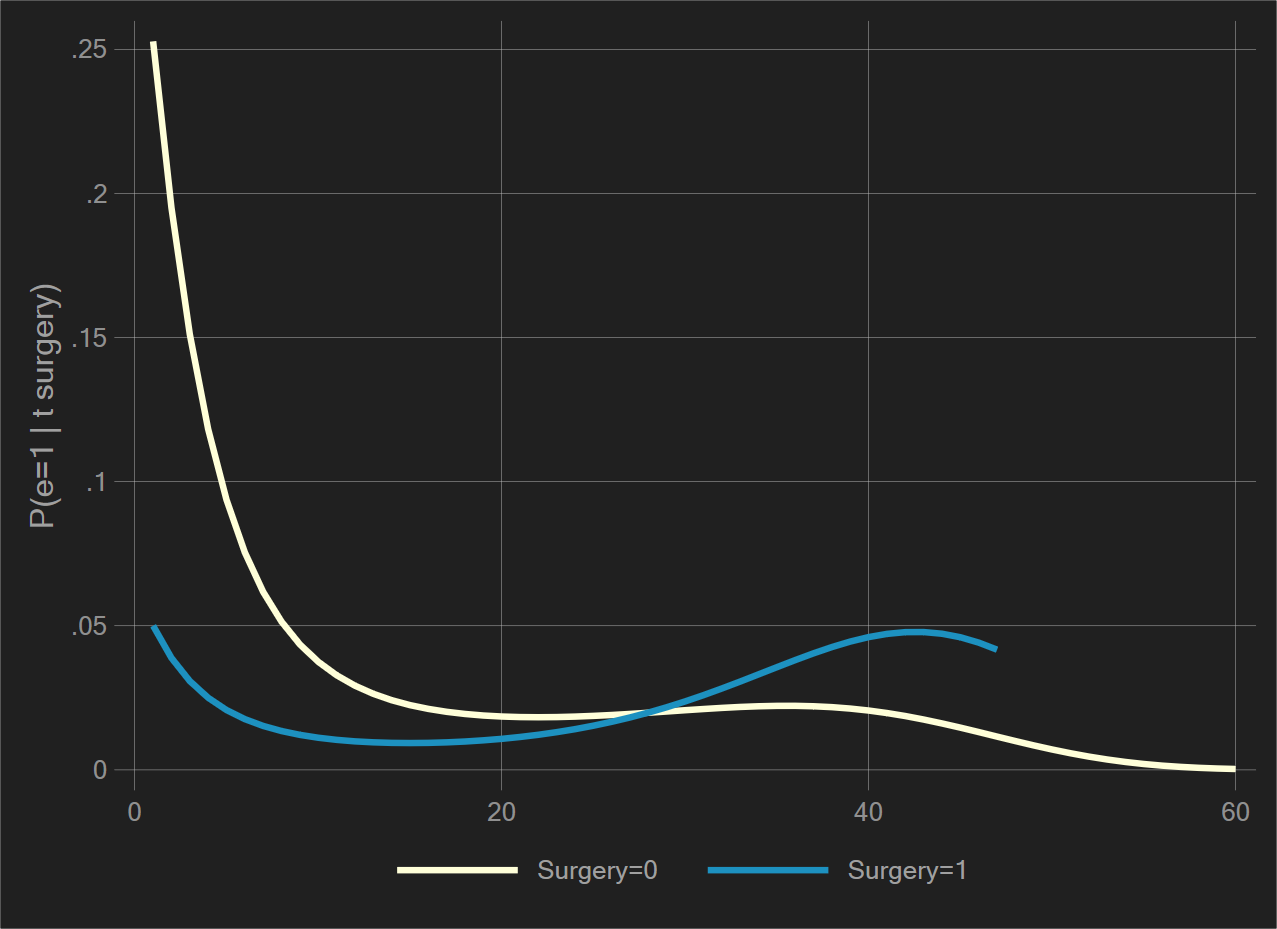
\includegraphics[width=0.7\textwidth,height=\textheight]{images/Image13.png}

}

\end{figure}

\hypertarget{variables-dynamiques}{%
\chapter{\texorpdfstring{\textbf{Variables
dynamiques}}{Variables dynamiques}}\label{variables-dynamiques}}

Cette section sera principalement traitée par l'exemple, et on ne
s'intéressera qu'aux variables de type discrète, avec un seul changement
d'état.

\begin{itemize}
\tightlist
\item
  Dans un modèle de durée, une variable dynamique peut-être appréhendée
  comme une intéraction entre la durée et une variable quantitative.
\item
  Pour un modèle de Cox, l'hypothèse de risque proportionnel ne peut
  donc pas être testée sur ce type de variable.
\item
  Ne pas tenir compte du caractère dynamique d'une dimension peut
  conduire à des interprétations erronées.
\item
  \textbf{\emph{Warning}}: La façon de modéliser les dimensions
  dynamiques en analyse des durées peut conduire à des biais de
  causalité, en particulier en sciences sociales, en omettant les
  \emph{effets d'anticipation}. C'est une situation classique avec des
  covariables dynamiques de type discrètes. Les techniques standards ne
  peuvent modéliser que des \emph{effets d'adaptation} : la cause -
  observée - précède l'effet.
\end{itemize}

\hypertarget{facteur-dynamique-traituxe9e-de-maniuxe8re-fixe}{%
\section{Facteur dynamique traitée de manière
fixe}\label{facteur-dynamique-traituxe9e-de-maniuxe8re-fixe}}

On reprend l'exemple sur malformation cardiaque, en ajoutant la variable
relative à la greffe. La question est donc de savoir si une
transplantation du coeur réduitle risque journalier de décéder (ou
augmente la durée de survie).\\
On a dans la base 2 variables: une variable binaire pour savoir si
l'individu à été greffé ou non, \textbf{transplant}, et la variable
\emph{wait} de type continue tronquée donnant la durée en jour jusqu'à
l'opération depuis l'inscription dans le registre (0 si
\(transplant=0\)).\\
On va dans un premier temps estimer le modèle de Cox avec la variable
fixe \emph{transplant}.

\begin{longtable}[]{@{}llllll@{}}
\caption{Modèle de cox avec une variable dynamique (binaire) traitée de
manière fixe (estimation biaisée}\tabularnewline
\toprule\noalign{}
Variables & HR & Std. err & z & P\textgreater\textbar z\textbar{} & 95\%
CI \\
\midrule\noalign{}
\endfirsthead
\toprule\noalign{}
Variables & HR & Std. err & z & P\textgreater\textbar z\textbar{} & 95\%
CI \\
\midrule\noalign{}
\endhead
\bottomrule\noalign{}
\endlastfoot
year & 0.910 & 0.060 & -1.42 & 0.155 & 0.799 ; 1.036 \\
age & 1.054 & 0.015 & 3.71 & 0.000 & 1.025 ; 1.084 \\
surgery & 0.541 & 0.243 & -1.37 & 0.171 & 0.224 ; 1.304 \\
transplant & 0.278 & 0.088 & -4.06 & 0.000 & 0.150 ; 0.515 \\
wait & 0.992 & 0.005 & -1.50 & 0.134 & 0.982 ; 1.002 \\
\end{longtable}

Interprétation: traitée de manière fixe, la greffe réduit donc
sensiblement le risque journalier de décéder (RR=0.278). De même on peut
admettre une certaine cohérence pour la durée jusqu'à la
transplantation: plus elle est précoce et plus les personnes survivent
(HR=0.992).

Sauf que\ldots..

Au niveau des données le modèle à été estimé, pour une personne greffée
(ici id=70), à partir de ce mapping:

\begin{longtable}[]{@{}lllllllll@{}}
\caption{Mapping de la base avec une variable dynamique binaire traitée
de manière fixe}\tabularnewline
\toprule\noalign{}
id & year & age & surgery & transplant & wait & died & \(t_0\) &
\(t\) \\
\midrule\noalign{}
\endfirsthead
\toprule\noalign{}
id & year & age & surgery & transplant & wait & died & \(t_0\) &
\(t\) \\
\midrule\noalign{}
\endhead
\bottomrule\noalign{}
\endlastfoot
70 & 72 & 52 & 0 & 1 & 5 & 0 & 0 & 1 \\
70 & 72 & 52 & 0 & 1 & 5 & 0 & 1 & 2 \\
70 & 72 & 52 & 0 & 1 & 5 & 0 & 2 & 3 \\
70 & 72 & 52 & 0 & 1 & 5 & 0 & 3 & 5 \\
70 & 72 & 52 & 0 & 1 & 5 & 0 & 5 & 6 \\
70 & 72 & 52 & 0 & 1 & 5 & 0 & 6 & 8 \\
70 & 72 & 52 & 0 & 1 & 5 & 0 & 8 & 9 \\
70 & 72 & 52 & 0 & 1 & 5 & 0 & 9 & 12 \\
70 & 72 & 52 & 0 & 1 & 5 & 0 & 12 & 16 \\
70 & 72 & 52 & 0 & 1 & 5 & 0 & 16 & 17 \\
70 & 72 & 52 & 0 & 1 & 5 & 0 & 17 & 18 \\
70 & 72 & 52 & 0 & 1 & 5 & 0 & 18 & 21 \\
70 & 72 & 52 & 0 & 1 & 5 & 0 & 21 & 28 \\
70 & 72 & 52 & 0 & 1 & 5 & 1 & 28 & 30 \\
\end{longtable}

Une personne est codée greffée avant le jour de la transplantation.
L'\textbf{\emph{effet causal}} est donc mal mesuré si sa dimension
temporelle a été ignorée, ici le jour exact de l'opération. C'est le
même principe pour l'évènement, la personne est codée décédée (1) le
jour du décès, et vivante avant (0).

\hypertarget{estimation-avec-une-variable-dynamique}{%
\section{Estimation avec une variable
dynamique}\label{estimation-avec-une-variable-dynamique}}

Il convient donc de modifier l'information avec le délai d'attente
jusqu'à la greffe. Le principe de construction de la variable dynamique,
quelle que soit le logiciel utilisé, doit suivre la logique suivante:

\(tvc = transplant\) , si \(transplant=1\) et \(t<wait\) alors \(tvc=0\)

\hypertarget{moduxe8le-de-cox}{%
\subsection{Modèle de Cox}\label{moduxe8le-de-cox}}

\begin{longtable}[]{@{}
  >{\raggedright\arraybackslash}p{(\columnwidth - 18\tabcolsep) * \real{0.0704}}
  >{\raggedright\arraybackslash}p{(\columnwidth - 18\tabcolsep) * \real{0.0845}}
  >{\raggedright\arraybackslash}p{(\columnwidth - 18\tabcolsep) * \real{0.0704}}
  >{\raggedright\arraybackslash}p{(\columnwidth - 18\tabcolsep) * \real{0.1268}}
  >{\raggedright\arraybackslash}p{(\columnwidth - 18\tabcolsep) * \real{0.1690}}
  >{\raggedright\arraybackslash}p{(\columnwidth - 18\tabcolsep) * \real{0.0845}}
  >{\raggedright\arraybackslash}p{(\columnwidth - 18\tabcolsep) * \real{0.0845}}
  >{\raggedright\arraybackslash}p{(\columnwidth - 18\tabcolsep) * \real{0.0986}}
  >{\raggedright\arraybackslash}p{(\columnwidth - 18\tabcolsep) * \real{0.0845}}
  >{\raggedright\arraybackslash}p{(\columnwidth - 18\tabcolsep) * \real{0.1268}}@{}}
\caption{Mapping correct de la base avec une variable dynamique
binaire}\tabularnewline
\toprule\noalign{}
\begin{minipage}[b]{\linewidth}\raggedright
id
\end{minipage} & \begin{minipage}[b]{\linewidth}\raggedright
year
\end{minipage} & \begin{minipage}[b]{\linewidth}\raggedright
age
\end{minipage} & \begin{minipage}[b]{\linewidth}\raggedright
surgery
\end{minipage} & \begin{minipage}[b]{\linewidth}\raggedright
transplant
\end{minipage} & \begin{minipage}[b]{\linewidth}\raggedright
wait
\end{minipage} & \begin{minipage}[b]{\linewidth}\raggedright
died
\end{minipage} & \begin{minipage}[b]{\linewidth}\raggedright
\(t_0\)
\end{minipage} & \begin{minipage}[b]{\linewidth}\raggedright
\(t\)
\end{minipage} & \begin{minipage}[b]{\linewidth}\raggedright
\textbf{TVC}
\end{minipage} \\
\midrule\noalign{}
\endfirsthead
\toprule\noalign{}
\begin{minipage}[b]{\linewidth}\raggedright
id
\end{minipage} & \begin{minipage}[b]{\linewidth}\raggedright
year
\end{minipage} & \begin{minipage}[b]{\linewidth}\raggedright
age
\end{minipage} & \begin{minipage}[b]{\linewidth}\raggedright
surgery
\end{minipage} & \begin{minipage}[b]{\linewidth}\raggedright
transplant
\end{minipage} & \begin{minipage}[b]{\linewidth}\raggedright
wait
\end{minipage} & \begin{minipage}[b]{\linewidth}\raggedright
died
\end{minipage} & \begin{minipage}[b]{\linewidth}\raggedright
\(t_0\)
\end{minipage} & \begin{minipage}[b]{\linewidth}\raggedright
\(t\)
\end{minipage} & \begin{minipage}[b]{\linewidth}\raggedright
\textbf{TVC}
\end{minipage} \\
\midrule\noalign{}
\endhead
\bottomrule\noalign{}
\endlastfoot
70 & 72 & 52 & 0 & 1 & 5 & 0 & 0 & 1 & \textbf{0} \\
70 & 72 & 52 & 0 & 1 & 5 & 0 & 1 & 2 & \textbf{0} \\
70 & 72 & 52 & 0 & 1 & 5 & 0 & 2 & 3 & \textbf{0} \\
70 & 72 & 52 & 0 & 1 & 5 & 0 & 3 & 5 & \textbf{0} \\
70 & 72 & 52 & 0 & 1 & 5 & 0 & 5 & 6 & \textbf{1} \\
70 & 72 & 52 & 0 & 1 & 5 & 0 & 6 & 8 & \textbf{1} \\
70 & 72 & 52 & 0 & 1 & 5 & 0 & 8 & 9 & \textbf{1} \\
70 & 72 & 52 & 0 & 1 & 5 & 0 & 9 & 12 & \textbf{1} \\
70 & 72 & 52 & 0 & 1 & 5 & 0 & 12 & 16 & \textbf{1} \\
70 & 72 & 52 & 0 & 1 & 5 & 0 & 16 & 17 & \textbf{1} \\
70 & 72 & 52 & 0 & 1 & 5 & 0 & 17 & 18 & \textbf{1} \\
70 & 72 & 52 & 0 & 1 & 5 & 0 & 18 & 21 & \textbf{1} \\
70 & 72 & 52 & 0 & 1 & 5 & 0 & 21 & 28 & \textbf{1} \\
70 & 72 & 52 & 0 & 1 & 5 & 1 & 28 & 30 & \textbf{1} \\
\end{longtable}

Si on estime maintenant le modèle avec cette variable dynamique qui
indique clairement le moment de la transition (jour de la greffe):

\begin{longtable}[]{@{}
  >{\raggedright\arraybackslash}p{(\columnwidth - 10\tabcolsep) * \real{0.3194}}
  >{\raggedright\arraybackslash}p{(\columnwidth - 10\tabcolsep) * \real{0.0972}}
  >{\raggedright\arraybackslash}p{(\columnwidth - 10\tabcolsep) * \real{0.1389}}
  >{\raggedright\arraybackslash}p{(\columnwidth - 10\tabcolsep) * \real{0.0972}}
  >{\raggedright\arraybackslash}p{(\columnwidth - 10\tabcolsep) * \real{0.1389}}
  >{\raggedright\arraybackslash}p{(\columnwidth - 10\tabcolsep) * \real{0.2083}}@{}}
\caption{Modèle de Cox avec une variable dynamique
binaire}\tabularnewline
\toprule\noalign{}
\begin{minipage}[b]{\linewidth}\raggedright
Variables
\end{minipage} & \begin{minipage}[b]{\linewidth}\raggedright
HR
\end{minipage} & \begin{minipage}[b]{\linewidth}\raggedright
Std. err
\end{minipage} & \begin{minipage}[b]{\linewidth}\raggedright
z
\end{minipage} & \begin{minipage}[b]{\linewidth}\raggedright
P\textgreater\textbar z\textbar{}
\end{minipage} & \begin{minipage}[b]{\linewidth}\raggedright
95\% CI
\end{minipage} \\
\midrule\noalign{}
\endfirsthead
\toprule\noalign{}
\begin{minipage}[b]{\linewidth}\raggedright
Variables
\end{minipage} & \begin{minipage}[b]{\linewidth}\raggedright
HR
\end{minipage} & \begin{minipage}[b]{\linewidth}\raggedright
Std. err
\end{minipage} & \begin{minipage}[b]{\linewidth}\raggedright
z
\end{minipage} & \begin{minipage}[b]{\linewidth}\raggedright
P\textgreater\textbar z\textbar{}
\end{minipage} & \begin{minipage}[b]{\linewidth}\raggedright
95\% CI
\end{minipage} \\
\midrule\noalign{}
\endhead
\bottomrule\noalign{}
\endlastfoot
\(year\) & 0.887 & 0.060 & -1.79 & 0.074 & 0.777 ; 1.012 \\
\(age\) & 1.031 & 0.014 & 2.19 & 0.029 & 1.003 ; 1.059 \\
\(surgery\) & 0.374 & 0.163 & -2.25 & 0.024 & 0.159 ; 0.880 \\
\(TVC transplantation\) & 0.921 & 0.281 & -0.27 & 0.787 & 0.507 ;
1.674 \\
\end{longtable}

L'impact de la greffe apparaît maintenant bien plus modéré sur la survie
des individus. Cela ne signifie pas non plus que des personnes ont pu
être \emph{sauvée} grâce à cette opération (ou plutôt leur durée de vie
augmentée), mais des complications lors de l'opération ou
post-opératoire, surtout à une époque où ces techniques étaient à leurs
balbutiements, ont pu également accélérer la mortalité. Il faut
également garder en tête que l'état de santé des personnes est
particulièrement dégradé, cette opération étant celle de la
\emph{dernière chance}.

R - Stata - Sas - Python

\subsection{Sas}

La base n'est pas modifiée et la création de la TVC est faite \emph{en
aveugle} dans la procédure \texttt{phreg}, après l'instruction
\texttt{model}. Ce n'est franchement pas super.

\subsection{R - Stata, Python}

La base doit être transformée en format long aux temps d'évènement
(\texttt{survsplit} avec R, \texttt{stsplit} avec Stata) avant la
création de la variable dynamique.

\hypertarget{moduxe8le-uxe0-temps-discret}{%
\subsection{Modèle à temps discret}\label{moduxe8le-uxe0-temps-discret}}

Même principe pour la construction de la variable dynamique. Pour rappel
l'échelle temporelle est le mois, on a créé en amont une variable qui
regroupe les valeurs de la variable \emph{wait} en périodes de 30 jours.

\begin{longtable}[]{@{}
  >{\raggedright\arraybackslash}p{(\columnwidth - 10\tabcolsep) * \real{0.2267}}
  >{\raggedright\arraybackslash}p{(\columnwidth - 10\tabcolsep) * \real{0.1200}}
  >{\raggedright\arraybackslash}p{(\columnwidth - 10\tabcolsep) * \real{0.1600}}
  >{\raggedright\arraybackslash}p{(\columnwidth - 10\tabcolsep) * \real{0.1200}}
  >{\raggedright\arraybackslash}p{(\columnwidth - 10\tabcolsep) * \real{0.1467}}
  >{\raggedright\arraybackslash}p{(\columnwidth - 10\tabcolsep) * \real{0.2267}}@{}}
\caption{Modèle logistique à durée discrète avec variable dynamique
binaire}\tabularnewline
\toprule\noalign{}
\begin{minipage}[b]{\linewidth}\raggedright
Variables
\end{minipage} & \begin{minipage}[b]{\linewidth}\raggedright
OR - RR
\end{minipage} & \begin{minipage}[b]{\linewidth}\raggedright
Std. err.
\end{minipage} & \begin{minipage}[b]{\linewidth}\raggedright
z
\end{minipage} & \begin{minipage}[b]{\linewidth}\raggedright
P\textgreater\textbar z\textbar{}
\end{minipage} & \begin{minipage}[b]{\linewidth}\raggedright
95\% IC
\end{minipage} \\
\midrule\noalign{}
\endfirsthead
\toprule\noalign{}
\begin{minipage}[b]{\linewidth}\raggedright
Variables
\end{minipage} & \begin{minipage}[b]{\linewidth}\raggedright
OR - RR
\end{minipage} & \begin{minipage}[b]{\linewidth}\raggedright
Std. err.
\end{minipage} & \begin{minipage}[b]{\linewidth}\raggedright
z
\end{minipage} & \begin{minipage}[b]{\linewidth}\raggedright
P\textgreater\textbar z\textbar{}
\end{minipage} & \begin{minipage}[b]{\linewidth}\raggedright
95\% IC
\end{minipage} \\
\midrule\noalign{}
\endhead
\bottomrule\noalign{}
\endlastfoot
\(t\) & 0.686 & 0.070 & -3.71 & 0.000 & 0.562 ; 0.837 \\
\(t^2\) & 1.015 & 0.006 & 2.53 & 0.011 & 1.003 ; 1.026 \\
\(t^3\) & 1.000 & 0.000 & -1.97 & 0.049 & 1.000 ; 1.000 \\
\(year\) & 0.876 & 0.065 & -1.79 & 0.073 & 0.758 ; 1.012 \\
\(age\) & 1.034 & 0.015 & 2.22 & 0.027 & 1.004 ; 1.064 \\
\(surgery\) & 0.363 & 0.163 & -2.25 & 0.024 & 0.151 ; 0.876 \\
\(TVC \; greffe\) & 1.029 & 0.355 & 0.08 & 0.934 & 0.524 ; 2.022 \\
& & & & & \\
\(Constante\) & \emph{0.440} & \emph{0.110} & \emph{-3.29} &
\emph{0.001} & \emph{0.270 ; 0.718} \\
\end{longtable}

\hypertarget{pruxe9cautions}{%
\section{Précautions}\label{pruxe9cautions}}

\begin{itemize}
\item
  Rappel: la cause doit précèder l'effet.
\item
  Lorsque l'évènement étudié n'est pas intrinsèquement de type absorbant
  comme le décès, la \emph{cause} peut se manifester ou plutôt être
  observée après la survenue de l'évènement étudié. Les modèles de durée
  standards ne peuvent pas gérer ces situations car l'observation sort
  du risque après la survenue de l'évènement. Il y a d'autres
  techniques, par exemple de type économétrique, qui sont plus à même de
  traiter ce genre de situations.
\item
  Même si la cause est bien mesurée avant l'évènement d'intérêt, un
  \emph{choc} n'est peut-être qu'un point final d'un processus causal
  antérieur: une séparation est rarement un évènement ponctuel, une
  phase plus ou moins longue de mésentente dans le couple lui a
  vraisemblablement préexister. La datation du début d'un processus
  causal n'est donc pas toujours facile à mesurer.

  \begin{itemize}
  \tightlist
  \item
    \textbf{Logique d'adaptation}: la \emph{cause} identifiée est
    mesurée avant l'évènement étudié.
  \item
    \textbf{Logique d'anticipation}: la \emph{cause} identifiée est
    mesurée après l'occurrence de l'évènement étudié. L'origine causale
    est bien antérieure à l'évènement, mais elle n'est pas directement
    observable.
  \end{itemize}
\item
  Lorsque les variables dynamiques sont de type quantitatives/continues,
  le problème on doit aussi considérer avec des phénomènes
  d'anticipation sur les valeurs attendues de ces variables, observées
  postérieurement à l'évènement étudié. On peut introduire des « lags »
  dans le modèle pour saisir ce phénomène : par exemple
  \(x_t= x_{t+1}\). Ce décalage des durées d'occurrence peut être aussi
  introduite pour les variables discrètes (naissance d'un enfant par
  exemple).
\end{itemize}

\part{Compléments}

\hypertarget{eluxe9ments-de-mise-en-forme-des-donnuxe9es}{%
\chapter{Eléments de mise en forme des
données}\label{eluxe9ments-de-mise-en-forme-des-donnuxe9es}}

Ce qui suit est un premier jet réalisé en 2023

Packages utilisés:

\begin{Shaded}
\begin{Highlighting}[]
\FunctionTok{library}\NormalTok{(dplyr)}
\FunctionTok{library}\NormalTok{(tidyr)}
\FunctionTok{library}\NormalTok{(knitr)}
\end{Highlighting}
\end{Shaded}

\hypertarget{calcul-des-variables-danalyses}{%
\section{Calcul des variables
d'analyses}\label{calcul-des-variables-danalyses}}

Construction de la base:

\begin{Shaded}
\begin{Highlighting}[]
\NormalTok{df }\OtherTok{=} \FunctionTok{data.frame}\NormalTok{(}\AttributeTok{id  =}  \FunctionTok{c}\NormalTok{(}\DecValTok{1}\NormalTok{, }\DecValTok{1}\NormalTok{, }\DecValTok{1}\NormalTok{, }\DecValTok{2}\NormalTok{),}
                \AttributeTok{deb =}  \FunctionTok{c}\NormalTok{(}\DecValTok{2020}\NormalTok{, }\DecValTok{2023}\NormalTok{, }\DecValTok{2024}\NormalTok{, }\DecValTok{2022}\NormalTok{),}
                \AttributeTok{fin =}  \FunctionTok{c}\NormalTok{(}\DecValTok{2021}\NormalTok{, }\DecValTok{2024}\NormalTok{, }\DecValTok{2025}\NormalTok{, }\ConstantTok{NA}\NormalTok{), }
                  \AttributeTok{x =}  \FunctionTok{c}\NormalTok{(}\DecValTok{1}\NormalTok{,}\DecValTok{2}\NormalTok{,}\DecValTok{1}\NormalTok{,}\DecValTok{2}\NormalTok{))}
\FunctionTok{kable}\NormalTok{(df)}
\end{Highlighting}
\end{Shaded}

\begin{longtable}[]{@{}rrrr@{}}
\toprule\noalign{}
id & deb & fin & x \\
\midrule\noalign{}
\endhead
\bottomrule\noalign{}
\endlastfoot
1 & 2020 & 2021 & 1 \\
1 & 2023 & 2024 & 2 \\
1 & 2024 & 2025 & 1 \\
2 & 2022 & NA & 2 \\
\end{longtable}

On supposera que l'année de collecte, pour toutes les observations, est
\textbf{2025} \footnote{Ici on a une enquête réalisée une même année
  pour toute les observations, ce n'est pas toujours le cas. De même au
  lieu de l'année, si les datations avaient été données par l'âge, au
  moment de l'enquête l'âge varierait d'une personne à une autre. Ces
  datations différentes (année ou âge) peuvent être présentes dans
  chaque module biographique d'une enquête, ou dans le fichier des
  caractéristiques fixes. Dans ce cas l'information devra être récupérée}.

Si cela n'est pas donné dans le module biographique, il peut être
intéressant de construire les numéros de séquences des trajectoires.

\begin{Shaded}
\begin{Highlighting}[]
\NormalTok{df}\SpecialCharTok{$}\NormalTok{nseq }\OtherTok{=} \DecValTok{1} 
\NormalTok{df }\OtherTok{=}\NormalTok{ df }\SpecialCharTok{\%\textgreater{}\%} \FunctionTok{group\_by}\NormalTok{(id) }\SpecialCharTok{\%\textgreater{}\%} \FunctionTok{mutate}\NormalTok{(}\AttributeTok{nseq =} \FunctionTok{cumsum}\NormalTok{(nseq))  }

\FunctionTok{kable}\NormalTok{(df)}
\end{Highlighting}
\end{Shaded}

\begin{longtable}[]{@{}rrrrr@{}}
\toprule\noalign{}
id & deb & fin & x & nseq \\
\midrule\noalign{}
\endhead
\bottomrule\noalign{}
\endlastfoot
1 & 2020 & 2021 & 1 & 1 \\
1 & 2023 & 2024 & 2 & 2 \\
1 & 2024 & 2025 & 1 & 3 \\
2 & 2022 & NA & 2 & 1 \\
\end{longtable}

\textbf{Exemple 1 : durée de séjour de la première séquence observée}

Supposons que x traduit un type de relation/union, par exemple x=1 est
une relation non cohabitante et x=2 est une relation cohabitante. On
s'intéresse à la durée de la première relation, sans distinction entre 1
et 2. Il suffit de séléctionner la première séquence.

\begin{Shaded}
\begin{Highlighting}[]
\NormalTok{df }\OtherTok{=} \FunctionTok{filter}\NormalTok{(df, nseq}\SpecialCharTok{==}\DecValTok{1}\NormalTok{)}
\end{Highlighting}
\end{Shaded}

La variable de fin va permettre de repérer les informations censurées,
et de générer la variable d'évènement. A ce niveau il est donc important
de ne pas encore remplacer la date de censure par sa valeur.

\begin{itemize}
\tightlist
\item
  Si \emph{fin} est une valeur manquante: observation censurée.
\item
  Si \emph{fin} est une valeur renseignée: occurence de l'évènement.
\end{itemize}

\begin{Shaded}
\begin{Highlighting}[]
\NormalTok{df}\SpecialCharTok{$}\NormalTok{e }\OtherTok{=} \FunctionTok{ifelse}\NormalTok{(}\FunctionTok{is.na}\NormalTok{(df}\SpecialCharTok{$}\NormalTok{fin), }\DecValTok{0}\NormalTok{,}\DecValTok{1}\NormalTok{)}

\FunctionTok{kable}\NormalTok{(df)}
\end{Highlighting}
\end{Shaded}

\begin{longtable}[]{@{}rrrrrr@{}}
\toprule\noalign{}
id & deb & fin & x & nseq & e \\
\midrule\noalign{}
\endhead
\bottomrule\noalign{}
\endlastfoot
1 & 2020 & 2021 & 1 & 1 & 1 \\
2 & 2022 & NA & 2 & 1 & 0 \\
\end{longtable}

Pour la variable de durée \footnote{La mesure est ici discrète/groupée,
  il me semble toujours préférable d'allonger les durées à +1. On
  démarre donc toujours un premier janvier pour terminer un 31 décembre
  sur l'information est donnée par des année. Ici t=1 représente la
  première année après la sortie des études. Une personne qui aura eu un
  emploi durant cette année, l'aura eu durant cette première année, que
  ce soit 2 semaines après ou 11 mois après. Si on disposait des mois,
  cela pourrait être intéressant de modifier cette métrique temporelle.
  Voir exemple 3}, une repéré les observations censurées, elle est
calculée directement avec les variables \emph{fin} et \emph{deb}.

\begin{Shaded}
\begin{Highlighting}[]
\NormalTok{df}\SpecialCharTok{$}\NormalTok{dur }\OtherTok{=} \FunctionTok{ifelse}\NormalTok{(df}\SpecialCharTok{$}\NormalTok{e}\SpecialCharTok{==}\DecValTok{1}\NormalTok{, df}\SpecialCharTok{$}\NormalTok{fin }\SpecialCharTok{{-}}\NormalTok{ df}\SpecialCharTok{$}\NormalTok{deb }\SpecialCharTok{+} \DecValTok{1}\NormalTok{, }\DecValTok{2025} \SpecialCharTok{{-}}\NormalTok{ df}\SpecialCharTok{$}\NormalTok{deb }\SpecialCharTok{+} \DecValTok{1}\NormalTok{)}

\FunctionTok{kable}\NormalTok{(df)}
\end{Highlighting}
\end{Shaded}

\begin{longtable}[]{@{}rrrrrrr@{}}
\toprule\noalign{}
id & deb & fin & x & nseq & e & dur \\
\midrule\noalign{}
\endhead
\bottomrule\noalign{}
\endlastfoot
1 & 2020 & 2021 & 1 & 1 & 1 & 2 \\
2 & 2022 & NA & 2 & 1 & 0 & 4 \\
\end{longtable}

\textbf{Exemple 2 : changement de métrique temporelle}

Toujours avec le même exemple, mais en ajoutant une observation,
supposons que l'on dispose également de l'information sur les mois. Sur
les mois où l'évènement à eu lieu, mais également sur les mois où
l'enquête a été réalisée.

\begin{Shaded}
\begin{Highlighting}[]
\NormalTok{df2 }\OtherTok{=} \FunctionTok{data.frame}\NormalTok{(}\AttributeTok{id  =} \FunctionTok{c}\NormalTok{(}\DecValTok{1}\NormalTok{, }\DecValTok{1}\NormalTok{, }\DecValTok{1}\NormalTok{, }\DecValTok{2}\NormalTok{,}\DecValTok{3}\NormalTok{),}
                \AttributeTok{deb  =} \FunctionTok{c}\NormalTok{(}\DecValTok{2020}\NormalTok{, }\DecValTok{2023}\NormalTok{, }\DecValTok{2024}\NormalTok{, }\DecValTok{2022}\NormalTok{, }\DecValTok{2021}\NormalTok{),}
                \AttributeTok{debm =} \FunctionTok{c}\NormalTok{(}\DecValTok{2}\NormalTok{,}\DecValTok{5}\NormalTok{,}\DecValTok{3}\NormalTok{,}\DecValTok{10}\NormalTok{,}\DecValTok{9}\NormalTok{),}
                \AttributeTok{fin  =} \FunctionTok{c}\NormalTok{(}\DecValTok{2021}\NormalTok{, }\DecValTok{2024}\NormalTok{, }\DecValTok{2025}\NormalTok{, }\ConstantTok{NA}\NormalTok{,}\DecValTok{2021}\NormalTok{), }
                \AttributeTok{finm =} \FunctionTok{c}\NormalTok{(}\DecValTok{4}\NormalTok{,}\DecValTok{2}\NormalTok{,}\DecValTok{12}\NormalTok{,}\ConstantTok{NA}\NormalTok{,}\DecValTok{11}\NormalTok{), }
                \AttributeTok{x    =} \FunctionTok{c}\NormalTok{(}\DecValTok{1}\NormalTok{,}\DecValTok{2}\NormalTok{,}\DecValTok{1}\NormalTok{,}\DecValTok{2}\NormalTok{,}\DecValTok{1}\NormalTok{),}
                \AttributeTok{enq  =} \FunctionTok{c}\NormalTok{(}\DecValTok{2025}\NormalTok{,}\DecValTok{2025}\NormalTok{,}\DecValTok{2025}\NormalTok{,}\DecValTok{2025}\NormalTok{,}\DecValTok{2025}\NormalTok{),}
                \AttributeTok{enqm =} \FunctionTok{c}\NormalTok{(}\DecValTok{4}\NormalTok{,}\DecValTok{4}\NormalTok{,}\DecValTok{4}\NormalTok{,}\DecValTok{5}\NormalTok{,}\DecValTok{4}\NormalTok{))}

\NormalTok{df2}\SpecialCharTok{$}\NormalTok{nseq }\OtherTok{=} \DecValTok{1} 
\NormalTok{df2 }\OtherTok{=}\NormalTok{ df2 }\SpecialCharTok{\%\textgreater{}\%} \FunctionTok{group\_by}\NormalTok{(id) }\SpecialCharTok{\%\textgreater{}\%} \FunctionTok{mutate}\NormalTok{(}\AttributeTok{nseq =} \FunctionTok{cumsum}\NormalTok{(nseq))  }

\FunctionTok{kable}\NormalTok{(df2)}
\end{Highlighting}
\end{Shaded}

\begin{longtable}[]{@{}rrrrrrrrr@{}}
\toprule\noalign{}
id & deb & debm & fin & finm & x & enq & enqm & nseq \\
\midrule\noalign{}
\endhead
\bottomrule\noalign{}
\endlastfoot
1 & 2020 & 2 & 2021 & 4 & 1 & 2025 & 4 & 1 \\
1 & 2023 & 5 & 2024 & 2 & 2 & 2025 & 4 & 2 \\
1 & 2024 & 3 & 2025 & 12 & 1 & 2025 & 4 & 3 \\
2 & 2022 & 10 & NA & NA & 2 & 2025 & 5 & 1 \\
3 & 2021 & 9 & 2021 & 11 & 1 & 2025 & 4 & 1 \\
\end{longtable}

On remarque que la nouvelle observation (id=3) a connu l'évènement, ici
la fin de la relation, la même année qu'au début d'exposition (le début
de la relation)\ldots. mais au bout de 2,6,11 mois???? Commeon dispose
de l'information sur les mois de début et de fin cela peut être
intéressant de l'exploite. De la même manière si l'enquête a été
réalisée la même année, les entretiens n'ont pas eu lieu le même mois.
On aura besoin de cette information pour les observations censurées.

De nouveau on sélectionne la première séquence, et pour la lisibilité de
la base on retire les informations qui ne seront pas ou plus exploitées
(\emph{nseq}, \emph{x}).

\begin{Shaded}
\begin{Highlighting}[]
\NormalTok{df2 }\OtherTok{=} \FunctionTok{filter}\NormalTok{(df2,nseq}\SpecialCharTok{==}\DecValTok{1}\NormalTok{)}
\NormalTok{df2 }\OtherTok{=} \FunctionTok{select}\NormalTok{(df2, }\SpecialCharTok{{-}}\FunctionTok{c}\NormalTok{(x,nseq))}

\FunctionTok{kable}\NormalTok{(df2)}
\end{Highlighting}
\end{Shaded}

\begin{longtable}[]{@{}rrrrrrr@{}}
\toprule\noalign{}
id & deb & debm & fin & finm & enq & enqm \\
\midrule\noalign{}
\endhead
\bottomrule\noalign{}
\endlastfoot
1 & 2020 & 2 & 2021 & 4 & 2025 & 4 \\
2 & 2022 & 10 & NA & NA & 2025 & 5 \\
3 & 2021 & 9 & 2021 & 11 & 2025 & 4 \\
\end{longtable}

On génère la variable censure/évènement (toujours à faire avant la
variable de durée) de la même manière que pour l'exemple 1.

\begin{Shaded}
\begin{Highlighting}[]
\NormalTok{df2}\SpecialCharTok{$}\NormalTok{e }\OtherTok{=} \FunctionTok{ifelse}\NormalTok{(}\FunctionTok{is.na}\NormalTok{(df2}\SpecialCharTok{$}\NormalTok{fin), }\DecValTok{0}\NormalTok{, }\DecValTok{1}\NormalTok{)}

\FunctionTok{kable}\NormalTok{(df2)}
\end{Highlighting}
\end{Shaded}

\begin{longtable}[]{@{}rrrrrrrr@{}}
\toprule\noalign{}
id & deb & debm & fin & finm & enq & enqm & e \\
\midrule\noalign{}
\endhead
\bottomrule\noalign{}
\endlastfoot
1 & 2020 & 2 & 2021 & 4 & 2025 & 4 & 1 \\
2 & 2022 & 10 & NA & NA & 2025 & 5 & 0 \\
3 & 2021 & 9 & 2021 & 11 & 2025 & 4 & 1 \\
\end{longtable}

Pour la variable de durée, le principe est de multiplié par 12 la
différence entre l'année de fin et l'année de début et d'ajouter la
différence entre le mois de fin et le mois de début.\\
Pour les observations censurées, ici l'année de fin est identique mais
les mois varient. En terme de programmation, surtout si avec R on
utilise \texttt{ifelse}, il est préférable d'y aller doucement en créant
une durée pour les observations qui ont connu l'évènement et une durée
pour les observations censurées. Puis de regrouper les deux cas. C'est
ce qui est fait dans le code qui suit.

Durée selon les valeurs de \emph{e}:

\begin{Shaded}
\begin{Highlighting}[]
\NormalTok{df2}\SpecialCharTok{$}\NormalTok{dur1 }\OtherTok{=} \FunctionTok{ifelse}\NormalTok{(df2}\SpecialCharTok{$}\NormalTok{e}\SpecialCharTok{==}\DecValTok{1}\NormalTok{, }\DecValTok{12}\SpecialCharTok{*}\NormalTok{(df2}\SpecialCharTok{$}\NormalTok{fin }\SpecialCharTok{{-}}\NormalTok{ df2}\SpecialCharTok{$}\NormalTok{deb) }\SpecialCharTok{+}\NormalTok{ (df2}\SpecialCharTok{$}\NormalTok{finm }\SpecialCharTok{{-}}\NormalTok{ df2}\SpecialCharTok{$}\NormalTok{debm),  }\DecValTok{0}\NormalTok{) }
\NormalTok{df2}\SpecialCharTok{$}\NormalTok{dur0 }\OtherTok{=} \FunctionTok{ifelse}\NormalTok{(df2}\SpecialCharTok{$}\NormalTok{e}\SpecialCharTok{==}\DecValTok{0}\NormalTok{, }\DecValTok{12}\SpecialCharTok{*}\NormalTok{(}\DecValTok{2025} \SpecialCharTok{{-}}\NormalTok{ df2}\SpecialCharTok{$}\NormalTok{deb)    }\SpecialCharTok{+}\NormalTok{ (df2}\SpecialCharTok{$}\NormalTok{enqm  }\SpecialCharTok{{-}}\NormalTok{ df2}\SpecialCharTok{$}\NormalTok{debm), }\DecValTok{0}\NormalTok{) }

\FunctionTok{kable}\NormalTok{(df2)}
\end{Highlighting}
\end{Shaded}

\begin{longtable}[]{@{}rrrrrrrrrr@{}}
\toprule\noalign{}
id & deb & debm & fin & finm & enq & enqm & e & dur1 & dur0 \\
\midrule\noalign{}
\endhead
\bottomrule\noalign{}
\endlastfoot
1 & 2020 & 2 & 2021 & 4 & 2025 & 4 & 1 & 14 & 0 \\
2 & 2022 & 10 & NA & NA & 2025 & 5 & 0 & 0 & 31 \\
3 & 2021 & 9 & 2021 & 11 & 2025 & 4 & 1 & 2 & 0 \\
\end{longtable}

On regroupe par simple sommation (le \emph{else} étant 0).

\begin{Shaded}
\begin{Highlighting}[]
\NormalTok{df2}\SpecialCharTok{$}\NormalTok{dur  }\OtherTok{=}\NormalTok{ df2}\SpecialCharTok{$}\NormalTok{dur1 }\SpecialCharTok{+}\NormalTok{ df2}\SpecialCharTok{$}\NormalTok{dur0}

\NormalTok{df2 }\OtherTok{=} \FunctionTok{select}\NormalTok{(df2, }\SpecialCharTok{{-}}\FunctionTok{c}\NormalTok{(dur1,dur0))}

\FunctionTok{kable}\NormalTok{(df2)}
\end{Highlighting}
\end{Shaded}

\begin{longtable}[]{@{}rrrrrrrrr@{}}
\toprule\noalign{}
id & deb & debm & fin & finm & enq & enqm & e & dur \\
\midrule\noalign{}
\endhead
\bottomrule\noalign{}
\endlastfoot
1 & 2020 & 2 & 2021 & 4 & 2025 & 4 & 1 & 14 \\
2 & 2022 & 10 & NA & NA & 2025 & 5 & 0 & 31 \\
3 & 2021 & 9 & 2021 & 11 & 2025 & 4 & 1 & 2 \\
\end{longtable}

On dispose ainsi des éléments nécessaire pour faire une analyse de durée
avec une métrique mensuelle \footnote{Contrairement au durée annuelle je
  n'ai pas ajouté 1 à chaque durée, ce qui est de nouveau envisageable
  par exemple si on veut explicitement indiquer les évènements qui ont
  lieu le premier mois. Pour id=3 la relation a t-elle durée du 1er
  septembre au 30 novembre, ou du 30 septembre au 1er novembre?? On a
  toujours un problème de précision, mais ici d'une trentaine de jours}.

\textbf{Exemple 3 : importation d'un début d'expositon externe}

On repart de la première base

\begin{longtable}[]{@{}rrrrr@{}}
\toprule\noalign{}
id & deb & fin & x & nseq \\
\midrule\noalign{}
\endhead
\bottomrule\noalign{}
\endlastfoot
1 & 2020 & 2021 & 1 & 1 \\
1 & 2023 & 2024 & 2 & 2 \\
1 & 2024 & 2025 & 1 & 3 \\
2 & 2022 & NA & 2 & 1 \\
\end{longtable}

On suppose maintenant que x traduit des situations sur le marché du
travail. Par exemple \textbf{x=1} est un emploi en CDD et \textbf{x=2}
un emploi en CDI. On s'intéresse à la durée entre la fin des études et
le premier emploi, quel que soit sont type.

\begin{itemize}
\tightlist
\item
  On ne dispose pas ici de toutes l'information pour calculer la durée,
  soit la fin des études. Elle peut être donnée dans une base classique
  regroupant l'ensemble des caractéristiques individuelles de type fixe
  (année de naissance, sexe\ldots).
\item
  Comme on s'intéresse à la durée de recherche du premier emploi, dans
  le module biographique la date de début va devenir la date de fin.
\item
  Pour les observations présente dans la base biographique, il n'y a pas
  de censure à droite. Mais si on regarde le fichier des
  caractéristiques générales, fixe:
\end{itemize}

\begin{Shaded}
\begin{Highlighting}[]
\NormalTok{etude }\OtherTok{=} \FunctionTok{data.frame}\NormalTok{(}\AttributeTok{id =} \FunctionTok{c}\NormalTok{(}\DecValTok{1}\NormalTok{,}\DecValTok{2}\NormalTok{,}\DecValTok{3}\NormalTok{), }\AttributeTok{fin\_etude =} \FunctionTok{c}\NormalTok{(}\DecValTok{2020}\NormalTok{,}\DecValTok{2021}\NormalTok{,}\DecValTok{2023}\NormalTok{))}
\FunctionTok{kable}\NormalTok{(etude)}
\end{Highlighting}
\end{Shaded}

\begin{longtable}[]{@{}rr@{}}
\toprule\noalign{}
id & fin\_etude \\
\midrule\noalign{}
\endhead
\bottomrule\noalign{}
\endlastfoot
1 & 2020 \\
2 & 2021 \\
3 & 2023 \\
\end{longtable}

Une nouvelle observation (id=3) apparaît. Au moment de l'enquête, elle
n'a pas (\textbf{encore}) trouvé un emploi depuis la fin de ces études.
On a donc une observation qui sera censurée.

\begin{tcolorbox}[enhanced jigsaw, arc=.35mm, bottomrule=.15mm, titlerule=0mm, colbacktitle=quarto-callout-note-color!10!white, left=2mm, opacitybacktitle=0.6, toprule=.15mm, title=\textcolor{quarto-callout-note-color}{\faInfo}\hspace{0.5em}{Note}, colframe=quarto-callout-note-color-frame, breakable, coltitle=black, opacityback=0, toptitle=1mm, bottomtitle=1mm, rightrule=.15mm, leftrule=.75mm, colback=white]

Certaines bases biographiques peuvent être structurées avec des
trajectoires strictement continue, l'année (l'âge) de fin étant l'année
(l'âge) de début de la trajectoire suivante. Dans ce cas, l'information
serait immédiatement disponible, avec la présence d'un nombre de
séquences plus important dans la base.

\end{tcolorbox}

On va devoir:

\begin{itemize}
\tightlist
\item
  Sélectionner la première sequence d'emploi dans la base df (variable
  \emph{nseq}).
\item
  La fusionner avec la base étude.
\end{itemize}

Avant la fusion, on peut conserver seulement les informations
nécessaires (id, deb). La variable \emph{deb} va changer également de
statut en devenant l'année de \emph{fin} de la période de recherche
d'emploi.

\begin{Shaded}
\begin{Highlighting}[]
\NormalTok{df }\OtherTok{=} \FunctionTok{filter}\NormalTok{(df, nseq}\SpecialCharTok{==}\DecValTok{1}\NormalTok{)}
\NormalTok{df }\OtherTok{=} \FunctionTok{select}\NormalTok{(df, }\SpecialCharTok{{-}}\FunctionTok{c}\NormalTok{(fin,x,nseq))}

\NormalTok{df }\OtherTok{=} \FunctionTok{rename}\NormalTok{(df, }\AttributeTok{fin =}\NormalTok{ deb)}
\FunctionTok{kable}\NormalTok{(df)}
\end{Highlighting}
\end{Shaded}

\begin{longtable}[]{@{}rr@{}}
\toprule\noalign{}
id & fin \\
\midrule\noalign{}
\endhead
\bottomrule\noalign{}
\endlastfoot
1 & 2020 \\
2 & 2022 \\
\end{longtable}

Après la fusion:

\begin{Shaded}
\begin{Highlighting}[]
\NormalTok{df }\OtherTok{=} \FunctionTok{full\_join}\NormalTok{(etude, df,  }\AttributeTok{by =} \FunctionTok{c}\NormalTok{(}\StringTok{\textquotesingle{}id\textquotesingle{}}\NormalTok{))}

\NormalTok{df }\OtherTok{=} \FunctionTok{rename}\NormalTok{(df, }\AttributeTok{deb =}\NormalTok{ fin\_etude)}

\FunctionTok{kable}\NormalTok{(df)}
\end{Highlighting}
\end{Shaded}

\begin{longtable}[]{@{}rrr@{}}
\toprule\noalign{}
id & deb & fin \\
\midrule\noalign{}
\endhead
\bottomrule\noalign{}
\endlastfoot
1 & 2020 & 2020 \\
2 & 2021 & 2022 \\
3 & 2023 & NA \\
\end{longtable}

On a toutes les informations pour générer la variable censure/évènement
et la variable de durée:

\begin{Shaded}
\begin{Highlighting}[]
\NormalTok{df}\SpecialCharTok{$}\NormalTok{e }\OtherTok{=} \FunctionTok{ifelse}\NormalTok{(}\FunctionTok{is.na}\NormalTok{(df}\SpecialCharTok{$}\NormalTok{fin),}\DecValTok{0}\NormalTok{,}\DecValTok{1}\NormalTok{)}

\NormalTok{df}\SpecialCharTok{$}\NormalTok{dur }\OtherTok{=} \FunctionTok{ifelse}\NormalTok{(df}\SpecialCharTok{$}\NormalTok{e, df}\SpecialCharTok{$}\NormalTok{fin }\SpecialCharTok{{-}}\NormalTok{ df}\SpecialCharTok{$}\NormalTok{deb }\SpecialCharTok{+} \DecValTok{1}\NormalTok{, }\DecValTok{2025} \SpecialCharTok{{-}}\NormalTok{ df}\SpecialCharTok{$}\NormalTok{deb }\SpecialCharTok{+} \DecValTok{1}\NormalTok{)}
\FunctionTok{kable}\NormalTok{(df)}
\end{Highlighting}
\end{Shaded}

\begin{longtable}[]{@{}rrrrr@{}}
\toprule\noalign{}
id & deb & fin & e & dur \\
\midrule\noalign{}
\endhead
\bottomrule\noalign{}
\endlastfoot
1 & 2020 & 2020 & 1 & 1 \\
2 & 2021 & 2022 & 1 & 2 \\
3 & 2023 & NA & 0 & 3 \\
\end{longtable}

\hypertarget{appariement-de-modules-biographiques}{%
\section{Appariement de modules
biographiques}\label{appariement-de-modules-biographiques}}

On repart de la première base, avec les numéros de séquence.

\begin{longtable}[]{@{}rrrrr@{}}
\toprule\noalign{}
id & deb & fin & x & nseq \\
\midrule\noalign{}
\endhead
\bottomrule\noalign{}
\endlastfoot
1 & 2020 & 2021 & 1 & 1 \\
1 & 2023 & 2024 & 2 & 2 \\
1 & 2024 & 2025 & 1 & 3 \\
2 & 2022 & NA & 2 & 1 \\
\end{longtable}

\hypertarget{mise-en-forme-dune-base}{%
\subsection{Mise en forme d'une base}\label{mise-en-forme-dune-base}}

Pour apparier des informations de plusieurs modules biographiques, on
doit transformer les bases en format individus-séquences en format
individus-périodes (ici individus années).

\begin{itemize}
\tightlist
\item
  \textbf{Etape 1}: allongement sur chaque séquence après avoir générées
  leur durée
\item
  \textbf{Etape 2}: générer une variable de période (année) sur chaque
  ligne. Elle servira pour l'appariement.
\end{itemize}

\textbf{Pourquoi ne pas utiliser la simple différence entre la fin et le
début ?}

Durée (fin - début) et allongement de la base:

On ne génère pas des variables d'analyse, on aurait besoin de
l'information sur l'année de l'enquête pour les informations censurées.

\begin{Shaded}
\begin{Highlighting}[]
\NormalTok{df}\SpecialCharTok{$}\NormalTok{fin[}\FunctionTok{is.na}\NormalTok{(df}\SpecialCharTok{$}\NormalTok{fin)] }\OtherTok{=} \DecValTok{2025}

\FunctionTok{kable}\NormalTok{(df)}
\end{Highlighting}
\end{Shaded}

\begin{longtable}[]{@{}rrrrr@{}}
\toprule\noalign{}
id & deb & fin & x & nseq \\
\midrule\noalign{}
\endhead
\bottomrule\noalign{}
\endlastfoot
1 & 2020 & 2021 & 1 & 1 \\
1 & 2023 & 2024 & 2 & 2 \\
1 & 2024 & 2025 & 1 & 3 \\
2 & 2022 & 2025 & 2 & 1 \\
\end{longtable}

Allongement de la base:

\begin{Shaded}
\begin{Highlighting}[]
\NormalTok{df1 }\OtherTok{=}\NormalTok{ df}
\NormalTok{df1}\SpecialCharTok{$}\NormalTok{dur1 }\OtherTok{=}\NormalTok{ df1}\SpecialCharTok{$}\NormalTok{fin }\SpecialCharTok{{-}}\NormalTok{ df1}\SpecialCharTok{$}\NormalTok{deb}

\NormalTok{df1}\SpecialCharTok{$}\NormalTok{dur1b }\OtherTok{=}\NormalTok{ df1}\SpecialCharTok{$}\NormalTok{dur1 }\CommentTok{\# uncount supprime la variable d\textquotesingle{}origine }
\NormalTok{df1 }\OtherTok{=} \FunctionTok{uncount}\NormalTok{(df1,dur1b)}

\FunctionTok{kable}\NormalTok{(df1)}
\end{Highlighting}
\end{Shaded}

\begin{longtable}[]{@{}rrrrrr@{}}
\toprule\noalign{}
id & deb & fin & x & nseq & dur1 \\
\midrule\noalign{}
\endhead
\bottomrule\noalign{}
\endlastfoot
1 & 2020 & 2021 & 1 & 1 & 1 \\
1 & 2023 & 2024 & 2 & 2 & 1 \\
1 & 2024 & 2025 & 1 & 3 & 1 \\
2 & 2022 & 2025 & 2 & 1 & 3 \\
2 & 2022 & 2025 & 2 & 1 & 3 \\
2 & 2022 & 2025 & 2 & 1 & 3 \\
\end{longtable}

Pour générer la variable période (année), on a besoin d'un compteur qui
sera associé à la variable \emph{deb}. On doit bien contrôler
l'opération par identifiant et numéro de séquence.

\begin{Shaded}
\begin{Highlighting}[]
\NormalTok{df1}\SpecialCharTok{$}\NormalTok{c }\OtherTok{=} \DecValTok{1}
\NormalTok{df1 }\OtherTok{=}\NormalTok{ df1 }\SpecialCharTok{\%\textgreater{}\%} \FunctionTok{group\_by}\NormalTok{(id,nseq) }\SpecialCharTok{\%\textgreater{}\%} \FunctionTok{mutate}\NormalTok{(}\AttributeTok{year =}\NormalTok{ deb  }\SpecialCharTok{+} \FunctionTok{cumsum}\NormalTok{(c)) }

\FunctionTok{kable}\NormalTok{(df1)}
\end{Highlighting}
\end{Shaded}

\begin{longtable}[]{@{}rrrrrrrr@{}}
\toprule\noalign{}
id & deb & fin & x & nseq & dur1 & c & year \\
\midrule\noalign{}
\endhead
\bottomrule\noalign{}
\endlastfoot
1 & 2020 & 2021 & 1 & 1 & 1 & 1 & 2021 \\
1 & 2023 & 2024 & 2 & 2 & 1 & 1 & 2024 \\
1 & 2024 & 2025 & 1 & 3 & 1 & 1 & 2025 \\
2 & 2022 & 2025 & 2 & 1 & 3 & 1 & 2023 \\
2 & 2022 & 2025 & 2 & 1 & 3 & 1 & 2024 \\
2 & 2022 & 2025 & 2 & 1 & 3 & 1 & 2025 \\
\end{longtable}

\textbf{Problème}: les années de début ne sont pas correncte: 2021 au
lieu de 2020 pour la première séquence de id=1 par exemple.

\begin{tcolorbox}[enhanced jigsaw, arc=.35mm, bottomrule=.15mm, titlerule=0mm, colbacktitle=quarto-callout-important-color!10!white, left=2mm, opacitybacktitle=0.6, toprule=.15mm, title=\textcolor{quarto-callout-important-color}{\faExclamation}\hspace{0.5em}{Important}, colframe=quarto-callout-important-color-frame, breakable, coltitle=black, opacityback=0, toptitle=1mm, bottomtitle=1mm, rightrule=.15mm, leftrule=.75mm, colback=white]

On doit donc impérativement augmenter la différence entre la fin et le
début par +1 pour que l'ensemble des périodes (années) soit couvertes.

\end{tcolorbox}

On reprend donc les opérations précédentes mais avec \textbf{durée = fin
- debut + 1}

\begin{itemize}
\tightlist
\item
  Allongement de la base avec durée augmentée
\end{itemize}

\begin{Shaded}
\begin{Highlighting}[]
\NormalTok{df2 }\OtherTok{=}\NormalTok{ df}
\NormalTok{df2}\SpecialCharTok{$}\NormalTok{dur2 }\OtherTok{=}\NormalTok{ df2}\SpecialCharTok{$}\NormalTok{fin }\SpecialCharTok{{-}}\NormalTok{ df2}\SpecialCharTok{$}\NormalTok{deb }\SpecialCharTok{+} \DecValTok{1}

\NormalTok{df2}\SpecialCharTok{$}\NormalTok{dur2b }\OtherTok{=}\NormalTok{ df2}\SpecialCharTok{$}\NormalTok{dur2 }\CommentTok{\# uncount supprime la variable d\textquotesingle{}origine }
\NormalTok{df2 }\OtherTok{=} \FunctionTok{uncount}\NormalTok{(df2,dur2b)}

\FunctionTok{kable}\NormalTok{(df2)}
\end{Highlighting}
\end{Shaded}

\begin{longtable}[]{@{}rrrrrr@{}}
\toprule\noalign{}
id & deb & fin & x & nseq & dur2 \\
\midrule\noalign{}
\endhead
\bottomrule\noalign{}
\endlastfoot
1 & 2020 & 2021 & 1 & 1 & 2 \\
1 & 2020 & 2021 & 1 & 1 & 2 \\
1 & 2023 & 2024 & 2 & 2 & 2 \\
1 & 2023 & 2024 & 2 & 2 & 2 \\
1 & 2024 & 2025 & 1 & 3 & 2 \\
1 & 2024 & 2025 & 1 & 3 & 2 \\
2 & 2022 & 2025 & 2 & 1 & 4 \\
2 & 2022 & 2025 & 2 & 1 & 4 \\
2 & 2022 & 2025 & 2 & 1 & 4 \\
2 & 2022 & 2025 & 2 & 1 & 4 \\
\end{longtable}

\begin{itemize}
\tightlist
\item
  Création de la variable \emph{year}: \textbf{sur chaque
  individus-séquences, la somme entre le compteur et l'année de début
  doit être réduite de 11}.
\end{itemize}

\begin{Shaded}
\begin{Highlighting}[]
\NormalTok{df2}\SpecialCharTok{$}\NormalTok{c }\OtherTok{=} \DecValTok{1}
\NormalTok{df2 }\OtherTok{=}\NormalTok{ df2 }\SpecialCharTok{\%\textgreater{}\%} \FunctionTok{group\_by}\NormalTok{(id,nseq) }\SpecialCharTok{\%\textgreater{}\%} \FunctionTok{mutate}\NormalTok{(}\AttributeTok{year =}\NormalTok{ deb  }\SpecialCharTok{+} \FunctionTok{cumsum}\NormalTok{(c) }\SpecialCharTok{{-}} \DecValTok{1}\NormalTok{)}

\NormalTok{df2 }\OtherTok{=} \FunctionTok{select}\NormalTok{(df2, }\SpecialCharTok{{-}}\FunctionTok{c}\NormalTok{(deb,fin,dur2))}


\FunctionTok{kable}\NormalTok{(df2)}
\end{Highlighting}
\end{Shaded}

\begin{longtable}[]{@{}rrrrr@{}}
\toprule\noalign{}
id & x & nseq & c & year \\
\midrule\noalign{}
\endhead
\bottomrule\noalign{}
\endlastfoot
1 & 1 & 1 & 1 & 2020 \\
1 & 1 & 1 & 1 & 2021 \\
1 & 2 & 2 & 1 & 2023 \\
1 & 2 & 2 & 1 & 2024 \\
1 & 1 & 3 & 1 & 2024 \\
1 & 1 & 3 & 1 & 2025 \\
2 & 2 & 1 & 1 & 2022 \\
2 & 2 & 1 & 1 & 2023 \\
2 & 2 & 1 & 1 & 2024 \\
2 & 2 & 1 & 1 & 2025 \\
\end{longtable}

Les années sont toutes couvertes\ldots.mais un peu trop. En effet,
lorsque les trajectoires sont continues soit lorsque l'année de fin
d'une séquence est identique à l'année de début de la suivante, les
années vont être doublonnées. On doit dont supprimer ce doublon.

\begin{itemize}
\tightlist
\item
  Suppression des doublons des trajectoires continues.
\end{itemize}

De nouveaux on doit faire un choix, soit on priviligie l'année de fin,
soit on privilégie l'année de début. Les applications ont des fonctions
qui permettent de supprimer les doublons\footnote{avec R par exemple la
  fonction \texttt{unique} de dplyr}. On peut le faire manuellement en
regardant pour chaque personnes-années le nombre de doublon. Cela se
fait facilement à l'aide d'un compteur, ici la variable \emph{nyear}.

\begin{Shaded}
\begin{Highlighting}[]
\NormalTok{df2 }\OtherTok{=}\NormalTok{ df2 }\SpecialCharTok{\%\textgreater{}\%} \FunctionTok{group\_by}\NormalTok{(id,year) }\SpecialCharTok{\%\textgreater{}\%} \FunctionTok{mutate}\NormalTok{(}\AttributeTok{nyear =} \FunctionTok{cumsum}\NormalTok{(c))}

\FunctionTok{kable}\NormalTok{(df2)}
\end{Highlighting}
\end{Shaded}

\begin{longtable}[]{@{}rrrrrr@{}}
\toprule\noalign{}
id & x & nseq & c & year & nyear \\
\midrule\noalign{}
\endhead
\bottomrule\noalign{}
\endlastfoot
1 & 1 & 1 & 1 & 2020 & 1 \\
1 & 1 & 1 & 1 & 2021 & 1 \\
1 & 2 & 2 & 1 & 2023 & 1 \\
1 & 2 & 2 & 1 & 2024 & 1 \\
1 & 1 & 3 & 1 & 2024 & 2 \\
1 & 1 & 3 & 1 & 2025 & 1 \\
2 & 2 & 1 & 1 & 2022 & 1 \\
2 & 2 & 1 & 1 & 2023 & 1 \\
2 & 2 & 1 & 1 & 2024 & 1 \\
2 & 2 & 1 & 1 & 2025 & 1 \\
\end{longtable}

Si on souhaite garder l'année de fin on filtre les observations en
conservant celles dont nyear=1. Si on souhaite privilégier les années de
début on foltre les observations en conservant celles dont nyear=2. Si
on souhaite conserver les années de fin de séquence:

\begin{Shaded}
\begin{Highlighting}[]
\NormalTok{df2 }\OtherTok{=} \FunctionTok{filter}\NormalTok{(df2, nyear}\SpecialCharTok{==}\DecValTok{1}\NormalTok{)}

\NormalTok{df2 }\OtherTok{=} \FunctionTok{select}\NormalTok{(df2, }\SpecialCharTok{{-}}\FunctionTok{c}\NormalTok{(nseq,c,nyear))}

\FunctionTok{kable}\NormalTok{(df2)}
\end{Highlighting}
\end{Shaded}

\begin{longtable}[]{@{}rrr@{}}
\toprule\noalign{}
id & x & year \\
\midrule\noalign{}
\endhead
\bottomrule\noalign{}
\endlastfoot
1 & 1 & 2020 \\
1 & 1 & 2021 \\
1 & 2 & 2023 \\
1 & 2 & 2024 \\
1 & 1 & 2025 \\
2 & 2 & 2022 \\
2 & 2 & 2023 \\
2 & 2 & 2024 \\
2 & 2 & 2025 \\
\end{longtable}

\begin{tcolorbox}[enhanced jigsaw, arc=.35mm, bottomrule=.15mm, titlerule=0mm, colbacktitle=quarto-callout-important-color!10!white, left=2mm, opacitybacktitle=0.6, toprule=.15mm, title=\textcolor{quarto-callout-important-color}{\faExclamation}\hspace{0.5em}{En résumé}, colframe=quarto-callout-important-color-frame, breakable, coltitle=black, opacityback=0, toptitle=1mm, bottomtitle=1mm, rightrule=.15mm, leftrule=.75mm, colback=white]

\begin{itemize}
\tightlist
\item
  A la date (année/âge) de censure remplacer la valeur manquante par sa
  valeur. Si ultérieurement on a besoin de garder l'information sur la
  censure - valeur manquante - , on peut générer une variable mirroir de
  \emph{fin}.
\item
  Sur chaque séquence calculer la durée avec une augmentation de +1.
\item
  Créer une variable période (année) sur chaque ligne. Elle servira à
  définir la clé d'appariement.
\item
  Supprimer les doublons sur les transition continue
  \(fin_t = debut_{t+1}\).
\end{itemize}

\end{tcolorbox}

\hypertarget{fusion-des-informations-biographiques}{%
\subsection{Fusion des informations
biographiques}\label{fusion-des-informations-biographiques}}

\hypertarget{fusion-avec-lensemble-des-puxe9riodes-observables}{%
\subsubsection{Fusion avec l'ensemble des périodes
observables}\label{fusion-avec-lensemble-des-puxe9riodes-observables}}

Pour commencer par un exemple plutôt simple, on note que pour id=1
l'année 2022 n'est pas renseignée (trajectoire non continue). Si on
reprend un exemple précédent (relations de couple), cette année pourrait
être identifiée comme une période sans relation. Une façon simple de
boucher ce type ``trous'', est d'utiliser les années de naissances des
individus, et de créer une base individus-périodes qui couvre toutes les
années de vie de l'individu jusqu'à l'enquête. On remontera jusque là,
mais on va par exemple considérer que pour id=1 et id=2 ce \emph{début
de tout} est en 2018.

\begin{Shaded}
\begin{Highlighting}[]
\NormalTok{dftout }\OtherTok{=} \FunctionTok{data.frame}\NormalTok{(}\AttributeTok{id  =}  \FunctionTok{c}\NormalTok{(}\DecValTok{1}\NormalTok{, }\DecValTok{2}\NormalTok{),}
                    \AttributeTok{t0  =}  \FunctionTok{c}\NormalTok{(}\DecValTok{2018}\NormalTok{, }\DecValTok{2018}\NormalTok{))}

\FunctionTok{kable}\NormalTok{(dftout)    }
\end{Highlighting}
\end{Shaded}

\begin{longtable}[]{@{}rr@{}}
\toprule\noalign{}
id & t0 \\
\midrule\noalign{}
\endhead
\bottomrule\noalign{}
\endlastfoot
1 & 2018 \\
2 & 2018 \\
\end{longtable}

\begin{itemize}
\tightlist
\item
  On ajoute l'information sur l'année de l'enquête (2025).
\item
  On génère la durée
\item
  On allonge la base
\item
  On génère la variable année sur chaque ligne (on contrôle seulement
  sur \emph{id})
\end{itemize}

\begin{Shaded}
\begin{Highlighting}[]
\NormalTok{dftout}\SpecialCharTok{$}\NormalTok{tmax }\OtherTok{=} \DecValTok{2025}

\NormalTok{dftout}\SpecialCharTok{$}\NormalTok{dur  }\OtherTok{=}\NormalTok{ dftout}\SpecialCharTok{$}\NormalTok{tmax }\SpecialCharTok{{-}}\NormalTok{ dftout}\SpecialCharTok{$}\NormalTok{t0 }\SpecialCharTok{+} \DecValTok{1}

\NormalTok{dftout }\OtherTok{=} \FunctionTok{uncount}\NormalTok{(dftout,dur)}


\NormalTok{dftout}\SpecialCharTok{$}\NormalTok{c }\OtherTok{=} \DecValTok{1}
\NormalTok{dftout }\OtherTok{=}\NormalTok{ dftout }\SpecialCharTok{\%\textgreater{}\%} \FunctionTok{group\_by}\NormalTok{(id) }\SpecialCharTok{\%\textgreater{}\%} \FunctionTok{mutate}\NormalTok{(}\AttributeTok{year =}\NormalTok{ t0  }\SpecialCharTok{+} \FunctionTok{cumsum}\NormalTok{(c) }\SpecialCharTok{{-}} \DecValTok{1}\NormalTok{)}

\NormalTok{dftout }\OtherTok{=} \FunctionTok{select}\NormalTok{(dftout, }\SpecialCharTok{{-}}\FunctionTok{c}\NormalTok{(t0,tmax,c))}

\FunctionTok{kable}\NormalTok{(dftout)    }
\end{Highlighting}
\end{Shaded}

\begin{longtable}[]{@{}rr@{}}
\toprule\noalign{}
id & year \\
\midrule\noalign{}
\endhead
\bottomrule\noalign{}
\endlastfoot
1 & 2018 \\
1 & 2019 \\
1 & 2020 \\
1 & 2021 \\
1 & 2022 \\
1 & 2023 \\
1 & 2024 \\
1 & 2025 \\
2 & 2018 \\
2 & 2019 \\
2 & 2020 \\
2 & 2021 \\
2 & 2022 \\
2 & 2023 \\
2 & 2024 \\
2 & 2025 \\
\end{longtable}

On peut maintenant apparier cette couverture de toutes les années de vie
jusqu'à l'enquête à la base biographique:

\begin{Shaded}
\begin{Highlighting}[]
\NormalTok{df2 }\OtherTok{=} \FunctionTok{full\_join}\NormalTok{(df2, dftout, }\AttributeTok{by =} \FunctionTok{c}\NormalTok{(}\StringTok{"id"}\NormalTok{,}\StringTok{"year"}\NormalTok{))}

\NormalTok{df2 }\OtherTok{=} \FunctionTok{arrange}\NormalTok{(df2, id, year)}
\FunctionTok{kable}\NormalTok{(df2)    }
\end{Highlighting}
\end{Shaded}

\begin{longtable}[]{@{}rrr@{}}
\toprule\noalign{}
id & x & year \\
\midrule\noalign{}
\endhead
\bottomrule\noalign{}
\endlastfoot
1 & NA & 2018 \\
1 & NA & 2019 \\
1 & 1 & 2020 \\
1 & 1 & 2021 \\
1 & NA & 2022 \\
1 & 2 & 2023 \\
1 & 2 & 2024 \\
1 & 1 & 2025 \\
2 & NA & 2018 \\
2 & NA & 2019 \\
2 & NA & 2020 \\
2 & NA & 2021 \\
2 & 2 & 2022 \\
2 & 2 & 2023 \\
2 & 2 & 2024 \\
2 & 2 & 2025 \\
\end{longtable}

Pour supprimer les informations qui précèdent la première séquence de la
biographie, on peut générer un compteur sur la variable x après avoir
remplacer ses valeurs manquantes par des 0. On gardera les lignes pour
lesquels ce compteur est supérieur à 1.

\begin{Shaded}
\begin{Highlighting}[]
\NormalTok{df2}\SpecialCharTok{$}\NormalTok{x[}\FunctionTok{is.na}\NormalTok{(df2}\SpecialCharTok{$}\NormalTok{x)] }\OtherTok{=} \DecValTok{0}

\NormalTok{df2 }\OtherTok{=}\NormalTok{ df2 }\SpecialCharTok{\%\textgreater{}\%} \FunctionTok{group\_by}\NormalTok{(id) }\SpecialCharTok{\%\textgreater{}\%} \FunctionTok{mutate}\NormalTok{(}\AttributeTok{nx =} \FunctionTok{cumsum}\NormalTok{(x))}

\FunctionTok{kable}\NormalTok{(df2)    }
\end{Highlighting}
\end{Shaded}

\begin{longtable}[]{@{}rrrr@{}}
\toprule\noalign{}
id & x & year & nx \\
\midrule\noalign{}
\endhead
\bottomrule\noalign{}
\endlastfoot
1 & 0 & 2018 & 0 \\
1 & 0 & 2019 & 0 \\
1 & 1 & 2020 & 1 \\
1 & 1 & 2021 & 2 \\
1 & 0 & 2022 & 2 \\
1 & 2 & 2023 & 4 \\
1 & 2 & 2024 & 6 \\
1 & 1 & 2025 & 7 \\
2 & 0 & 2018 & 0 \\
2 & 0 & 2019 & 0 \\
2 & 0 & 2020 & 0 \\
2 & 0 & 2021 & 0 \\
2 & 2 & 2022 & 2 \\
2 & 2 & 2023 & 4 \\
2 & 2 & 2024 & 6 \\
2 & 2 & 2025 & 8 \\
\end{longtable}

On supprime les lignes lorsque nx=0.

\begin{Shaded}
\begin{Highlighting}[]
\NormalTok{df2 }\OtherTok{=} \FunctionTok{filter}\NormalTok{(df2, nx}\SpecialCharTok{\textgreater{}}\DecValTok{0}\NormalTok{)}

\NormalTok{df2 }\OtherTok{=} \FunctionTok{select}\NormalTok{(df2, }\SpecialCharTok{{-}}\FunctionTok{c}\NormalTok{(nx))}

\FunctionTok{kable}\NormalTok{(df2)    }
\end{Highlighting}
\end{Shaded}

\begin{longtable}[]{@{}rrr@{}}
\toprule\noalign{}
id & x & year \\
\midrule\noalign{}
\endhead
\bottomrule\noalign{}
\endlastfoot
1 & 1 & 2020 \\
1 & 1 & 2021 \\
1 & 0 & 2022 \\
1 & 2 & 2023 \\
1 & 2 & 2024 \\
1 & 1 & 2025 \\
2 & 2 & 2022 \\
2 & 2 & 2023 \\
2 & 2 & 2024 \\
2 & 2 & 2025 \\
\end{longtable}

\hypertarget{fusion-avec-une-autre-base-biographique}{%
\subsubsection{Fusion avec une autre base
biographique}\label{fusion-avec-une-autre-base-biographique}}

On peut être amené à fusionner plusieurs modules biographique. Jusqu'à
présent, une même année, tous les individus ne pouvaient être que dans
une situation, par exemple une seul emploi, un seul lieu de résidence
etc\ldots{} Pour certains phénomènes, une même années ou pendant une
période plus longue on peut observer simultanément plusieurs états
différent, ou plus classiquement observer une somme d'un même état. On
parle ici d'\textbf{\emph{overlapping}}. Ce type de situation est
typiquement celle qu'on observe avec le nombre d'enfants.

Supposons que le base ci-dessous traduit la naissance et potentiellement
le décès des enfants.

\begin{Shaded}
\begin{Highlighting}[]
\NormalTok{dfy }\OtherTok{=} \FunctionTok{data.frame}\NormalTok{(}\AttributeTok{id  =}  \FunctionTok{c}\NormalTok{(}\DecValTok{1}\NormalTok{, }\DecValTok{2}\NormalTok{, }\DecValTok{2}\NormalTok{),}
                \AttributeTok{deb =}  \FunctionTok{c}\NormalTok{(}\DecValTok{2022}\NormalTok{, }\DecValTok{2019}\NormalTok{, }\DecValTok{2023}\NormalTok{),}
                \AttributeTok{fin =}  \FunctionTok{c}\NormalTok{(}\ConstantTok{NA}\NormalTok{, }\DecValTok{2024}\NormalTok{,}\ConstantTok{NA}\NormalTok{), }
                \AttributeTok{nseq =}  \FunctionTok{c}\NormalTok{(}\DecValTok{1}\NormalTok{,}\DecValTok{1}\NormalTok{,}\DecValTok{2}\NormalTok{))}

\FunctionTok{kable}\NormalTok{(dfy)}
\end{Highlighting}
\end{Shaded}

\begin{longtable}[]{@{}rrrr@{}}
\toprule\noalign{}
id & deb & fin & nseq \\
\midrule\noalign{}
\endhead
\bottomrule\noalign{}
\endlastfoot
1 & 2022 & NA & 1 \\
2 & 2019 & 2024 & 1 \\
2 & 2023 & NA & 2 \\
\end{longtable}

\begin{itemize}
\tightlist
\item
  id=1 a un premier enfant en 2022 qui est toujours en vie au moment de
  l'enquête (2025)
\item
  id=2:

  \begin{itemize}
  \tightlist
  \item
    A un premier enfant en 2019 qui décède en 2024
  \item
    A un second enfant en 2023, toujours en vie au moment de l'enquête
  \item
    De la naissance du second enfant au décès du premier, on va donc
    avoir des doublons (overlapping) sur les années
  \end{itemize}
\end{itemize}

Si on reprend les manipulations précédentes jusqu'à la création de la
variable \emph{year}:

\begin{Shaded}
\begin{Highlighting}[]
\NormalTok{dfy}\SpecialCharTok{$}\NormalTok{fin[}\FunctionTok{is.na}\NormalTok{(dfy}\SpecialCharTok{$}\NormalTok{fin)] }\OtherTok{=} \DecValTok{2025}
\NormalTok{dfy}\SpecialCharTok{$}\NormalTok{dur }\OtherTok{=}\NormalTok{ dfy}\SpecialCharTok{$}\NormalTok{fin }\SpecialCharTok{{-}}\NormalTok{ dfy}\SpecialCharTok{$}\NormalTok{deb }\SpecialCharTok{+} \DecValTok{1}

\NormalTok{dfy}\SpecialCharTok{$}\NormalTok{durb }\OtherTok{=}\NormalTok{ dfy}\SpecialCharTok{$}\NormalTok{dur  }\CommentTok{\# Uncount supprime la variable d\textquotesingle{}origine }
\NormalTok{dfy }\OtherTok{=} \FunctionTok{uncount}\NormalTok{(dfy,durb)}

\NormalTok{dfy}\SpecialCharTok{$}\NormalTok{c }\OtherTok{=} \DecValTok{1}
\NormalTok{dfy }\OtherTok{=}\NormalTok{ dfy }\SpecialCharTok{\%\textgreater{}\%} \FunctionTok{group\_by}\NormalTok{(id,nseq) }\SpecialCharTok{\%\textgreater{}\%} \FunctionTok{mutate}\NormalTok{(}\AttributeTok{year =}\NormalTok{ deb  }\SpecialCharTok{+} \FunctionTok{cumsum}\NormalTok{(c) }\SpecialCharTok{{-}} \DecValTok{1}\NormalTok{)}
\end{Highlighting}
\end{Shaded}

La variable \emph{year} est bien renseignée 2 fois pour les années 2023
et 2024.

On peut s'intéresser au fait d'avoir ou non un enfant, ou de manière
plus générale au nombre d'enfant. En créant cette information, on se
donne également le moyen de corriger cet overlapping:

\begin{itemize}
\tightlist
\item
  On peut de nouveau générer un compteur contrôlé par individu année
\item
  En génerant un total de ligne doublonnée, on récupèrera par exemple
  ici le nombre d'enfant en vie chaque année.
\item
  En ne gardant que la ligne ou le compteur est égal à 1, on supprime
  les doublons tout en gardant l'information sur le nombre d'enfant en
  vie une année donnée.
\end{itemize}

\begin{Shaded}
\begin{Highlighting}[]
\NormalTok{dfy }\OtherTok{=}\NormalTok{ dfy }\SpecialCharTok{\%\textgreater{}\%} \FunctionTok{group\_by}\NormalTok{(id,year) }\SpecialCharTok{\%\textgreater{}\%} \FunctionTok{mutate}\NormalTok{(}\AttributeTok{ny =} \FunctionTok{cumsum}\NormalTok{(c))}
\NormalTok{dfy }\OtherTok{=}\NormalTok{ dfy }\SpecialCharTok{\%\textgreater{}\%} \FunctionTok{group\_by}\NormalTok{(id,year) }\SpecialCharTok{\%\textgreater{}\%} \FunctionTok{mutate}\NormalTok{(}\AttributeTok{tot\_y =}  \FunctionTok{sum}\NormalTok{(c))}

\FunctionTok{kable}\NormalTok{(dfy)}
\end{Highlighting}
\end{Shaded}

\begin{longtable}[]{@{}rrrrrrrrr@{}}
\toprule\noalign{}
id & deb & fin & nseq & dur & c & year & ny & tot\_y \\
\midrule\noalign{}
\endhead
\bottomrule\noalign{}
\endlastfoot
1 & 2022 & 2025 & 1 & 4 & 1 & 2022 & 1 & 1 \\
1 & 2022 & 2025 & 1 & 4 & 1 & 2023 & 1 & 1 \\
1 & 2022 & 2025 & 1 & 4 & 1 & 2024 & 1 & 1 \\
1 & 2022 & 2025 & 1 & 4 & 1 & 2025 & 1 & 1 \\
2 & 2019 & 2024 & 1 & 6 & 1 & 2019 & 1 & 1 \\
2 & 2019 & 2024 & 1 & 6 & 1 & 2020 & 1 & 1 \\
2 & 2019 & 2024 & 1 & 6 & 1 & 2021 & 1 & 1 \\
2 & 2019 & 2024 & 1 & 6 & 1 & 2022 & 1 & 1 \\
2 & 2019 & 2024 & 1 & 6 & 1 & 2023 & 1 & 2 \\
2 & 2019 & 2024 & 1 & 6 & 1 & 2024 & 1 & 2 \\
2 & 2023 & 2025 & 2 & 3 & 1 & 2023 & 2 & 2 \\
2 & 2023 & 2025 & 2 & 3 & 1 & 2024 & 2 & 2 \\
2 & 2023 & 2025 & 2 & 3 & 1 & 2025 & 1 & 1 \\
\end{longtable}

Il ne reste plus qu'à supprimer les lignes où \emph{ny\textgreater1}

\begin{Shaded}
\begin{Highlighting}[]
\NormalTok{dfy }\OtherTok{=} \FunctionTok{filter}\NormalTok{(dfy, ny}\SpecialCharTok{==}\DecValTok{1}\NormalTok{)}
\NormalTok{dfy }\OtherTok{=} \FunctionTok{select}\NormalTok{(dfy, }\SpecialCharTok{{-}}\FunctionTok{c}\NormalTok{(ny,deb, fin, dur, nseq, c))}

\FunctionTok{kable}\NormalTok{(dfy)}
\end{Highlighting}
\end{Shaded}

\begin{longtable}[]{@{}rrr@{}}
\toprule\noalign{}
id & year & tot\_y \\
\midrule\noalign{}
\endhead
\bottomrule\noalign{}
\endlastfoot
1 & 2022 & 1 \\
1 & 2023 & 1 \\
1 & 2024 & 1 \\
1 & 2025 & 1 \\
2 & 2019 & 1 \\
2 & 2020 & 1 \\
2 & 2021 & 1 \\
2 & 2022 & 1 \\
2 & 2023 & 2 \\
2 & 2024 & 2 \\
2 & 2025 & 1 \\
\end{longtable}

Avec une ligne par année, on peut la fusionner avec une autre base
biographique en format individus-années (même principe qu'avec la fusion
avec la base sur toutes les années de vie).

\begin{Shaded}
\begin{Highlighting}[]
\NormalTok{df2y }\OtherTok{=} \FunctionTok{full\_join}\NormalTok{(dfy, df2, }\AttributeTok{by =} \FunctionTok{c}\NormalTok{(}\StringTok{"id"}\NormalTok{,}\StringTok{"year"}\NormalTok{))}

\NormalTok{df2y }\OtherTok{=} \FunctionTok{arrange}\NormalTok{(df2y, id,year)}

\NormalTok{df2y }\OtherTok{=} \FunctionTok{select}\NormalTok{(df2y, }\FunctionTok{c}\NormalTok{(id,year,x,tot\_y))}

\NormalTok{df2y}\SpecialCharTok{$}\NormalTok{tot\_y[}\FunctionTok{is.na}\NormalTok{(df2y}\SpecialCharTok{$}\NormalTok{tot\_y)] }\OtherTok{=} \DecValTok{0}
\NormalTok{df2y}\SpecialCharTok{$}\NormalTok{x[}\FunctionTok{is.na}\NormalTok{(df2y}\SpecialCharTok{$}\NormalTok{x)]   }\OtherTok{=} \DecValTok{0}

\FunctionTok{kable}\NormalTok{(df2y)}
\end{Highlighting}
\end{Shaded}

\begin{longtable}[]{@{}rrrr@{}}
\toprule\noalign{}
id & year & x & tot\_y \\
\midrule\noalign{}
\endhead
\bottomrule\noalign{}
\endlastfoot
1 & 2020 & 1 & 0 \\
1 & 2021 & 1 & 0 \\
1 & 2022 & 0 & 1 \\
1 & 2023 & 2 & 1 \\
1 & 2024 & 2 & 1 \\
1 & 2025 & 1 & 1 \\
2 & 2019 & 0 & 1 \\
2 & 2020 & 0 & 1 \\
2 & 2021 & 0 & 1 \\
2 & 2022 & 2 & 1 \\
2 & 2023 & 2 & 2 \\
2 & 2024 & 2 & 2 \\
2 & 2025 & 2 & 1 \\
\end{longtable}

\hypertarget{suxe9lection-dun-type-de-suxe9quence-et-mise-en-forme-pour-lanalyse}{%
\section{Sélection d'un type de séquence et mise en forme pour
l'analyse}\label{suxe9lection-dun-type-de-suxe9quence-et-mise-en-forme-pour-lanalyse}}

\hypertarget{duruxe9e-jusquuxe0-la-premiuxe8re-suxe9quence}{%
\section{Durée jusqu'à la première
séquence}\label{duruxe9e-jusquuxe0-la-premiuxe8re-suxe9quence}}

\begin{Shaded}
\begin{Highlighting}[]
\NormalTok{df }\OtherTok{=}  \FunctionTok{data.frame}\NormalTok{(}\AttributeTok{id  =}  \FunctionTok{c}\NormalTok{( }\DecValTok{1}\NormalTok{, }\DecValTok{1}\NormalTok{, }\DecValTok{1}\NormalTok{, }\DecValTok{2}\NormalTok{, }\DecValTok{3}\NormalTok{, }\DecValTok{3}\NormalTok{, }\DecValTok{4}\NormalTok{),}
                 \AttributeTok{deb =}  \FunctionTok{c}\NormalTok{(}\DecValTok{2018}\NormalTok{, }\DecValTok{2022}\NormalTok{, }\DecValTok{2024}\NormalTok{, }\DecValTok{2019}\NormalTok{, }\DecValTok{2023}\NormalTok{, }\DecValTok{2024}\NormalTok{, }\DecValTok{2023}\NormalTok{),}
                 \AttributeTok{fin =}  \FunctionTok{c}\NormalTok{(}\DecValTok{2021}\NormalTok{, }\DecValTok{2024}\NormalTok{, }\DecValTok{2025}\NormalTok{, }\ConstantTok{NA}\NormalTok{, }\DecValTok{2024}\NormalTok{, }\ConstantTok{NA}\NormalTok{, }\ConstantTok{NA}\NormalTok{), }
                 \AttributeTok{y  =}   \FunctionTok{c}\NormalTok{(}\DecValTok{1}\NormalTok{, }\DecValTok{2}\NormalTok{, }\DecValTok{1}\NormalTok{, }\DecValTok{2}\NormalTok{, }\DecValTok{3}\NormalTok{, }\DecValTok{2}\NormalTok{, }\DecValTok{1}\NormalTok{),}
                 \AttributeTok{nseq =} \FunctionTok{c}\NormalTok{(}\DecValTok{1}\NormalTok{, }\DecValTok{2}\NormalTok{, }\DecValTok{3}\NormalTok{, }\DecValTok{1}\NormalTok{, }\DecValTok{1}\NormalTok{, }\DecValTok{2}\NormalTok{, }\DecValTok{1}\NormalTok{)}
\NormalTok{                 )}

\FunctionTok{kable}\NormalTok{(df)}
\end{Highlighting}
\end{Shaded}

\begin{longtable}[]{@{}rrrrr@{}}
\toprule\noalign{}
id & deb & fin & y & nseq \\
\midrule\noalign{}
\endhead
\bottomrule\noalign{}
\endlastfoot
1 & 2018 & 2021 & 1 & 1 \\
1 & 2022 & 2024 & 2 & 2 \\
1 & 2024 & 2025 & 1 & 3 \\
2 & 2019 & NA & 2 & 1 \\
3 & 2023 & 2024 & 3 & 1 \\
3 & 2024 & NA & 2 & 2 \\
4 & 2023 & NA & 1 & 1 \\
\end{longtable}

On va s'intéresser à la durée jusqu'à l'occurence de la séquence de type
2 ou 3 (variable \emph{y}). On considéra que le début de l'exposition
est donné par la variable \emph{deb} sur la première séquence.

\begin{itemize}
\tightlist
\item
  id=1: début de l'exposition/observation en 2018, observe l'évènement
  en 2022.
\item
  id=2: début de l'exposition/observation en 2019, observe l'évènement
  la même année.
\item
  id=3: début de l'exposition/observation en 2019, observe l'évènement
  la même année.
\item
  id=4: début de l'exposition/observation en 2023, n'a pas connu
  l'évènement au moment de l'enquête.
\end{itemize}

\textbf{Recupération de l'année de l'évènement}

On peut repérer la présence d'une des deux séquences d'intérêt avec une
indicatrice.

\begin{Shaded}
\begin{Highlighting}[]
\NormalTok{df}\SpecialCharTok{$}\NormalTok{e }\OtherTok{=} \FunctionTok{ifelse}\NormalTok{(df}\SpecialCharTok{$}\NormalTok{y}\SpecialCharTok{==}\DecValTok{2} \SpecialCharTok{|}\NormalTok{ df}\SpecialCharTok{$}\NormalTok{y}\SpecialCharTok{==}\DecValTok{3}\NormalTok{,}\DecValTok{1}\NormalTok{,}\DecValTok{0}\NormalTok{)}

\FunctionTok{kable}\NormalTok{(df)}
\end{Highlighting}
\end{Shaded}

\begin{longtable}[]{@{}rrrrrr@{}}
\toprule\noalign{}
id & deb & fin & y & nseq & e \\
\midrule\noalign{}
\endhead
\bottomrule\noalign{}
\endlastfoot
1 & 2018 & 2021 & 1 & 1 & 0 \\
1 & 2022 & 2024 & 2 & 2 & 1 \\
1 & 2024 & 2025 & 1 & 3 & 0 \\
2 & 2019 & NA & 2 & 1 & 1 \\
3 & 2023 & 2024 & 3 & 1 & 1 \\
3 & 2024 & NA & 2 & 2 & 1 \\
4 & 2023 & NA & 1 & 1 & 0 \\
\end{longtable}

De nouveau l'utilisation d'un compteur sur cette variable indicatrice,
peut s'avérer utile pour repérer le moment de l'occurence.

\begin{Shaded}
\begin{Highlighting}[]
\NormalTok{df }\OtherTok{=}\NormalTok{ df }\SpecialCharTok{\%\textgreater{}\%} \FunctionTok{group\_by}\NormalTok{(id) }\SpecialCharTok{\%\textgreater{}\%} \FunctionTok{mutate}\NormalTok{(}\AttributeTok{n  =} \FunctionTok{cumsum}\NormalTok{(e)) }

\FunctionTok{kable}\NormalTok{(df)}
\end{Highlighting}
\end{Shaded}

\begin{longtable}[]{@{}rrrrrrr@{}}
\toprule\noalign{}
id & deb & fin & y & nseq & e & n \\
\midrule\noalign{}
\endhead
\bottomrule\noalign{}
\endlastfoot
1 & 2018 & 2021 & 1 & 1 & 0 & 0 \\
1 & 2022 & 2024 & 2 & 2 & 1 & 1 \\
1 & 2024 & 2025 & 1 & 3 & 0 & 1 \\
2 & 2019 & NA & 2 & 1 & 1 & 1 \\
3 & 2023 & 2024 & 3 & 1 & 1 & 1 \\
3 & 2024 & NA & 2 & 2 & 1 & 2 \\
4 & 2023 & NA & 1 & 1 & 0 & 0 \\
\end{longtable}

Pour id=(2,3,4), ce compteur permet d'obtenir l'information souhaitée, à
savoir n=0 en situation d'attente/séjour/survie et n=1 l'année de
l'évènement. Pour id=1 cependant, l'alternance en y=1 et y=(2,3) ne
permet pas de récupérer l'année d'occurence (première fois en 2 ou 3).
Cela peut être fait, en faisant un compteur sur le compteur précédent:

\begin{Shaded}
\begin{Highlighting}[]
\NormalTok{df }\OtherTok{=}\NormalTok{ df }\SpecialCharTok{\%\textgreater{}\%} \FunctionTok{group\_by}\NormalTok{(id) }\SpecialCharTok{\%\textgreater{}\%} \FunctionTok{mutate}\NormalTok{(}\AttributeTok{nn  =} \FunctionTok{cumsum}\NormalTok{(n)) }

\FunctionTok{kable}\NormalTok{(df)}
\end{Highlighting}
\end{Shaded}

\begin{longtable}[]{@{}rrrrrrrr@{}}
\toprule\noalign{}
id & deb & fin & y & nseq & e & n & nn \\
\midrule\noalign{}
\endhead
\bottomrule\noalign{}
\endlastfoot
1 & 2018 & 2021 & 1 & 1 & 0 & 0 & 0 \\
1 & 2022 & 2024 & 2 & 2 & 1 & 1 & 1 \\
1 & 2024 & 2025 & 1 & 3 & 0 & 1 & 2 \\
2 & 2019 & NA & 2 & 1 & 1 & 1 & 1 \\
3 & 2023 & 2024 & 3 & 1 & 1 & 1 & 1 \\
3 & 2024 & NA & 2 & 2 & 1 & 2 & 3 \\
4 & 2023 & NA & 1 & 1 & 0 & 0 & 0 \\
\end{longtable}

\textbf{Récupération des information censurée}

Pour récupérer l'information sur les observations qui seront censurée,
on peut faire un total sur la variable \emph{n} ou \emph{e}: si n=0,
l'individu n'aura pas connu l'évènement.

\begin{Shaded}
\begin{Highlighting}[]
\NormalTok{df }\OtherTok{=}\NormalTok{ df }\SpecialCharTok{\%\textgreater{}\%} \FunctionTok{group\_by}\NormalTok{(id) }\SpecialCharTok{\%\textgreater{}\%} \FunctionTok{mutate}\NormalTok{(}\AttributeTok{N  =} \FunctionTok{sum}\NormalTok{(n)) }

\FunctionTok{kable}\NormalTok{(df)}
\end{Highlighting}
\end{Shaded}

\begin{longtable}[]{@{}rrrrrrrrr@{}}
\toprule\noalign{}
id & deb & fin & y & nseq & e & n & nn & N \\
\midrule\noalign{}
\endhead
\bottomrule\noalign{}
\endlastfoot
1 & 2018 & 2021 & 1 & 1 & 0 & 0 & 0 & 2 \\
1 & 2022 & 2024 & 2 & 2 & 1 & 1 & 1 & 2 \\
1 & 2024 & 2025 & 1 & 3 & 0 & 1 & 2 & 2 \\
2 & 2019 & NA & 2 & 1 & 1 & 1 & 1 & 1 \\
3 & 2023 & 2024 & 3 & 1 & 1 & 1 & 1 & 3 \\
3 & 2024 & NA & 2 & 2 & 1 & 2 & 3 & 3 \\
4 & 2023 & NA & 1 & 1 & 0 & 0 & 0 & 0 \\
\end{longtable}

Pour id=4, N est bien égal à 0.

\textbf{Récupération du début de l'exposition}

Le début de l'exposition étant ici l'année de début de la première
séquence. On peut facilement récupérer cette sur toute les lignes en la
repérant (ici en générant une nouvelle variable avec la fonction
\texttt{ifelse}), et en sommant sa valeur sur les autres lignes (=0).

\hypertarget{annotated-cell-48}{%
\label{annotated-cell-48}}%
\begin{Shaded}
\begin{Highlighting}[]
\NormalTok{df}\SpecialCharTok{$}\NormalTok{ debexp }\OtherTok{=} \FunctionTok{ifelse}\NormalTok{(df}\SpecialCharTok{$}\NormalTok{nseq}\SpecialCharTok{==}\DecValTok{1}\NormalTok{, df}\SpecialCharTok{$}\NormalTok{deb, }\DecValTok{0}\NormalTok{)                    }\hspace*{\fill}\NormalTok{\circled{1}}
                    
\NormalTok{df }\OtherTok{=}\NormalTok{ df }\SpecialCharTok{\%\textgreater{}\%} \FunctionTok{group\_by}\NormalTok{(id) }\SpecialCharTok{\%\textgreater{}\%} \FunctionTok{mutate}\NormalTok{(}\AttributeTok{debexp  =} \FunctionTok{sum}\NormalTok{(debexp))    }\hspace*{\fill}\NormalTok{\circled{2}}

\FunctionTok{kable}\NormalTok{(df)}
\end{Highlighting}
\end{Shaded}

\begin{description}
\tightlist
\item[\circled{1}]
La variable \emph{debex} est égale à \emph{deb} si \emph{nseq=1}, 0
sinon.
\item[\circled{2}]
On somme cette valeur sur chaque individu pour l'ajouter aux séquences
suivantes.
\end{description}

\begin{longtable}[]{@{}rrrrrrrrrr@{}}
\toprule\noalign{}
id & deb & fin & y & nseq & e & n & nn & N & debexp \\
\midrule\noalign{}
\endhead
\bottomrule\noalign{}
\endlastfoot
1 & 2018 & 2021 & 1 & 1 & 0 & 0 & 0 & 2 & 2018 \\
1 & 2022 & 2024 & 2 & 2 & 1 & 1 & 1 & 2 & 2018 \\
1 & 2024 & 2025 & 1 & 3 & 0 & 1 & 2 & 2 & 2018 \\
2 & 2019 & NA & 2 & 1 & 1 & 1 & 1 & 1 & 2019 \\
3 & 2023 & 2024 & 3 & 1 & 1 & 1 & 1 & 3 & 2023 \\
3 & 2024 & NA & 2 & 2 & 1 & 2 & 3 & 3 & 2023 \\
4 & 2023 & NA & 1 & 1 & 0 & 0 & 0 & 0 & 2023 \\
\end{longtable}

\textbf{Mise en forme finale de la base}

On peut maintenant conserver les lignes qui nous intéresse à savoir
celle où \emph{nn=1} (évènement) ou \emph{N=0} (censure).

\begin{Shaded}
\begin{Highlighting}[]
\NormalTok{df }\OtherTok{=} \FunctionTok{filter}\NormalTok{(df, nn}\SpecialCharTok{==}\DecValTok{1} \SpecialCharTok{|}\NormalTok{ N}\SpecialCharTok{==}\DecValTok{0}\NormalTok{)}

\FunctionTok{kable}\NormalTok{(df)}
\end{Highlighting}
\end{Shaded}

\begin{longtable}[]{@{}rrrrrrrrrr@{}}
\toprule\noalign{}
id & deb & fin & y & nseq & e & n & nn & N & debexp \\
\midrule\noalign{}
\endhead
\bottomrule\noalign{}
\endlastfoot
1 & 2022 & 2024 & 2 & 2 & 1 & 1 & 1 & 2 & 2018 \\
2 & 2019 & NA & 2 & 1 & 1 & 1 & 1 & 1 & 2019 \\
3 & 2023 & 2024 & 3 & 1 & 1 & 1 & 1 & 3 & 2023 \\
4 & 2023 & NA & 1 & 1 & 0 & 0 & 0 & 0 & 2023 \\
\end{longtable}

On dispose déjà de la variable d'évènement/censure (\emph{e} ou \emph{n}
= (0,1), on finit donc par la variable de durée.

\begin{Shaded}
\begin{Highlighting}[]
\NormalTok{df}\SpecialCharTok{$}\NormalTok{fin[}\FunctionTok{is.na}\NormalTok{(df}\SpecialCharTok{$}\NormalTok{fin)] }\OtherTok{=} \DecValTok{2025}

\NormalTok{df}\SpecialCharTok{$}\NormalTok{dur }\OtherTok{=} \FunctionTok{ifelse}\NormalTok{(df}\SpecialCharTok{$}\NormalTok{e}\SpecialCharTok{==}\DecValTok{1}\NormalTok{, df}\SpecialCharTok{$}\NormalTok{deb }\SpecialCharTok{{-}}\NormalTok{ df}\SpecialCharTok{$}\NormalTok{debexp }\SpecialCharTok{+} \DecValTok{1}\NormalTok{, df}\SpecialCharTok{$}\NormalTok{fin }\SpecialCharTok{{-}}\NormalTok{ df}\SpecialCharTok{$}\NormalTok{debexp }\SpecialCharTok{+} \DecValTok{1}\NormalTok{)}

\NormalTok{df }\OtherTok{=} \FunctionTok{select}\NormalTok{(df, }\FunctionTok{c}\NormalTok{(id,e,dur))}

\FunctionTok{kable}\NormalTok{(df)}
\end{Highlighting}
\end{Shaded}

\begin{longtable}[]{@{}rrr@{}}
\toprule\noalign{}
id & e & dur \\
\midrule\noalign{}
\endhead
\bottomrule\noalign{}
\endlastfoot
1 & 1 & 5 \\
2 & 1 & 1 \\
3 & 1 & 1 \\
4 & 0 & 3 \\
\end{longtable}

Ces informations sont suffisantes pour estimer une fonction de séjour et
on peut ajouter, si elles ne sont pas présentes, des covariables fixes
issues du fichier des caractéristiques générales. Pour l'ajout de
covariables dynamiques, leur ajout n'est pas forcément difficile pour
une analyse en durée discrète \footnote{En conservant l'information sur
  les années, on transformera la base en format individu-période et on
  procédera à une fusion des informations}. Pour les analyses type Cox,
selon la nature de la variable dynamique, l'opération (quel que soit le
logiciel utilisé) risque d'être plus ou moins compliquée.

\hypertarget{duruxe9e-de-suxe9jour-dans-la-suxe9quence-dintuxe9ruxeat-et-variables-danalyse}{%
\section{Durée de séjour dans la séquence d'intérêt et variables
d'analyse}\label{duruxe9e-de-suxe9jour-dans-la-suxe9quence-dintuxe9ruxeat-et-variables-danalyse}}

En première ou deuxième analyse, on peut également voir s'intéresser à
la durée de séjour dans l'état précédent. Par exemple, si l'analyse
précédent consistait à regarder la durée de séjour dans le premier
emploi, on pourrait regarder ensuite la durée jusqu'à sa reprise.

Cela va un peu (voir plus) se compliquer. On va repartir de la base de
départ précédente en ajoutant une observation.

\begin{Shaded}
\begin{Highlighting}[]
\NormalTok{df }\OtherTok{=}  \FunctionTok{data.frame}\NormalTok{(}\AttributeTok{id  =}  \FunctionTok{c}\NormalTok{( }\DecValTok{1}\NormalTok{, }\DecValTok{1}\NormalTok{, }\DecValTok{1}\NormalTok{, }\DecValTok{2}\NormalTok{, }\DecValTok{3}\NormalTok{, }\DecValTok{3}\NormalTok{, }\DecValTok{4}\NormalTok{, }\DecValTok{5}\NormalTok{, }\DecValTok{5}\NormalTok{, }\DecValTok{5}\NormalTok{ , }\DecValTok{5}\NormalTok{),}
                 \AttributeTok{deb =}  \FunctionTok{c}\NormalTok{(}\DecValTok{2018}\NormalTok{, }\DecValTok{2022}\NormalTok{, }\DecValTok{2024}\NormalTok{, }\DecValTok{2019}\NormalTok{, }\DecValTok{2023}\NormalTok{, }\DecValTok{2024}\NormalTok{, }\DecValTok{2023}\NormalTok{, }\DecValTok{2019}\NormalTok{, }\DecValTok{2021}\NormalTok{, }\DecValTok{2023}\NormalTok{, }\DecValTok{2024}\NormalTok{),}
                 \AttributeTok{fin =}  \FunctionTok{c}\NormalTok{(}\DecValTok{2021}\NormalTok{, }\DecValTok{2024}\NormalTok{, }\DecValTok{2025}\NormalTok{, }\ConstantTok{NA}\NormalTok{, }\DecValTok{2024}\NormalTok{, }\ConstantTok{NA}\NormalTok{, }\ConstantTok{NA}\NormalTok{, }\DecValTok{2021}\NormalTok{, }\DecValTok{2023}\NormalTok{, }\DecValTok{2024}\NormalTok{, }\ConstantTok{NA}\NormalTok{), }
                 \AttributeTok{y  =}   \FunctionTok{c}\NormalTok{(}\DecValTok{1}\NormalTok{, }\DecValTok{2}\NormalTok{, }\DecValTok{1}\NormalTok{, }\DecValTok{2}\NormalTok{, }\DecValTok{3}\NormalTok{, }\DecValTok{2}\NormalTok{, }\DecValTok{1}\NormalTok{, }\DecValTok{1}\NormalTok{, }\DecValTok{2}\NormalTok{, }\DecValTok{1}\NormalTok{,}\DecValTok{3}\NormalTok{),}
                 \AttributeTok{nseq =} \FunctionTok{c}\NormalTok{(}\DecValTok{1}\NormalTok{, }\DecValTok{2}\NormalTok{, }\DecValTok{3}\NormalTok{, }\DecValTok{1}\NormalTok{, }\DecValTok{1}\NormalTok{, }\DecValTok{2}\NormalTok{, }\DecValTok{1}\NormalTok{, }\DecValTok{1}\NormalTok{, }\DecValTok{2}\NormalTok{, }\DecValTok{3}\NormalTok{, }\DecValTok{4}\NormalTok{)}
\NormalTok{)}

\FunctionTok{kable}\NormalTok{(df)}
\end{Highlighting}
\end{Shaded}

\begin{longtable}[]{@{}rrrrr@{}}
\toprule\noalign{}
id & deb & fin & y & nseq \\
\midrule\noalign{}
\endhead
\bottomrule\noalign{}
\endlastfoot
1 & 2018 & 2021 & 1 & 1 \\
1 & 2022 & 2024 & 2 & 2 \\
1 & 2024 & 2025 & 1 & 3 \\
2 & 2019 & NA & 2 & 1 \\
3 & 2023 & 2024 & 3 & 1 \\
3 & 2024 & NA & 2 & 2 \\
4 & 2023 & NA & 1 & 1 \\
5 & 2019 & 2021 & 1 & 1 \\
5 & 2021 & 2023 & 2 & 2 \\
5 & 2023 & 2024 & 1 & 3 \\
5 & 2024 & NA & 3 & 4 \\
\end{longtable}

\textbf{Filtrage des observations hors champs}

On peut déjà supprimer les observations hors champs, à savoir ici id=4
qui n'a pas connu l'évènement dont on analyse la durée.

\hypertarget{annotated-cell-52}{%
\label{annotated-cell-52}}%
\begin{Shaded}
\begin{Highlighting}[]
\NormalTok{df}\SpecialCharTok{$}\NormalTok{e23 }\OtherTok{=} \FunctionTok{ifelse}\NormalTok{(df}\SpecialCharTok{$}\NormalTok{y}\SpecialCharTok{==}\DecValTok{2} \SpecialCharTok{|}\NormalTok{ df}\SpecialCharTok{$}\NormalTok{y}\SpecialCharTok{==}\DecValTok{3}\NormalTok{,}\DecValTok{1}\NormalTok{,}\DecValTok{0}\NormalTok{)                       }\hspace*{\fill}\NormalTok{\circled{1}}

\NormalTok{df }\OtherTok{=}\NormalTok{ df }\SpecialCharTok{\%\textgreater{}\%}  \FunctionTok{group\_by}\NormalTok{(id) }\SpecialCharTok{\%\textgreater{}\%} \FunctionTok{mutate}\NormalTok{(}\AttributeTok{n23  =} \FunctionTok{cumsum}\NormalTok{(e23)) }
\NormalTok{df }\OtherTok{=} \FunctionTok{filter}\NormalTok{(df, n23}\SpecialCharTok{!=}\DecValTok{0}\NormalTok{)                                      }\hspace*{\fill}\NormalTok{\circled{2}}

\FunctionTok{kable}\NormalTok{(df)}
\end{Highlighting}
\end{Shaded}

\begin{description}
\tightlist
\item[\circled{1}]
Nom de la variable \emph{e23} pour repérer la présence de l'évènement
dont on analyse la durée.
\item[\circled{2}]
Ce compteur est suffisant car l'observation n'a qu'une ligne.
\end{description}

\begin{longtable}[]{@{}rrrrrrr@{}}
\toprule\noalign{}
id & deb & fin & y & nseq & e23 & n23 \\
\midrule\noalign{}
\endhead
\bottomrule\noalign{}
\endlastfoot
1 & 2022 & 2024 & 2 & 2 & 1 & 1 \\
1 & 2024 & 2025 & 1 & 3 & 0 & 1 \\
2 & 2019 & NA & 2 & 1 & 1 & 1 \\
3 & 2023 & 2024 & 3 & 1 & 1 & 1 \\
3 & 2024 & NA & 2 & 2 & 1 & 2 \\
5 & 2021 & 2023 & 2 & 2 & 1 & 1 \\
5 & 2023 & 2024 & 1 & 3 & 0 & 1 \\
5 & 2024 & NA & 3 & 4 & 1 & 2 \\
\end{longtable}

\textbf{Récupération de l'évènement analysé}

Ici l'évènement sera un \emph{retour} dans l'état y=1. Il y a de nouveau
une possibilité de censure à droite si une observation reste dans l'état
2 ou 3 jusqu'au moment de l'enquête.

Il peut être utile d'utiliser des variables décalées pour repérer les
changements d'état d'une séquence à une autre. Ces décalages sont
appelées \emph{lead} ou \emph{lag}:

\begin{itemize}
\tightlist
\item
  \textbf{\emph{lead}}: \(x_t = x_{t+1}\)
\item
  \textbf{\emph{lag}}: \(x_t = x_{t-1}\)
\end{itemize}

On va utilise ici des \textbf{\emph{lead}} et donc pouvoir repérer les
changements d'état d'une séquence à une autre. Comme on s'intéresse au
retour à l'état 1:

\hypertarget{annotated-cell-53}{%
\label{annotated-cell-53}}%
\begin{Shaded}
\begin{Highlighting}[]
\NormalTok{df}\SpecialCharTok{$}\NormalTok{e }\OtherTok{=} \FunctionTok{ifelse}\NormalTok{(df}\SpecialCharTok{$}\NormalTok{y}\SpecialCharTok{==}\DecValTok{1}\NormalTok{,}\DecValTok{1}\NormalTok{,}\DecValTok{0}\NormalTok{)                                     }\hspace*{\fill}\NormalTok{\circled{1}}

\NormalTok{df }\OtherTok{=}\NormalTok{ df }\SpecialCharTok{\%\textgreater{}\%}  \FunctionTok{group\_by}\NormalTok{(id) }\SpecialCharTok{\%\textgreater{}\%} \FunctionTok{mutate}\NormalTok{(}\AttributeTok{diff\_e  =}\NormalTok{ e }\SpecialCharTok{{-}} \FunctionTok{lead}\NormalTok{(e))    }\hspace*{\fill}\NormalTok{\circled{2}}

\FunctionTok{kable}\NormalTok{(df)}
\end{Highlighting}
\end{Shaded}

\begin{description}
\tightlist
\item[\circled{1}]
\emph{e} est une indicatrice qui repère l'état 1
\item[\circled{2}]
On fait \emph{redescendre} la valeur de \emph{e} sur la séquence
précédente, et on calcule la difference.
\end{description}

\begin{longtable}[]{@{}rrrrrrrrr@{}}
\toprule\noalign{}
id & deb & fin & y & nseq & e23 & n23 & e & diff\_e \\
\midrule\noalign{}
\endhead
\bottomrule\noalign{}
\endlastfoot
1 & 2022 & 2024 & 2 & 2 & 1 & 1 & 0 & -1 \\
1 & 2024 & 2025 & 1 & 3 & 0 & 1 & 1 & NA \\
2 & 2019 & NA & 2 & 1 & 1 & 1 & 0 & NA \\
3 & 2023 & 2024 & 3 & 1 & 1 & 1 & 0 & 0 \\
3 & 2024 & NA & 2 & 2 & 1 & 2 & 0 & NA \\
5 & 2021 & 2023 & 2 & 2 & 1 & 1 & 0 & -1 \\
5 & 2023 & 2024 & 1 & 3 & 0 & 1 & 1 & 1 \\
5 & 2024 & NA & 3 & 4 & 1 & 2 & 0 & NA \\
\end{longtable}

Pour chaque dernière séquence la valeur du lag est une valeur manquante.
On repère l'évènement avec une valeur de -1 (transition de 0 à 1). On ne
peut pas encore filtrer les informations car il va falloir récupérer la
fin de la séquence, mais on peut déjà construire l'information.

\begin{Shaded}
\begin{Highlighting}[]
\NormalTok{df}\SpecialCharTok{$}\NormalTok{e }\OtherTok{=} \FunctionTok{ifelse}\NormalTok{(df}\SpecialCharTok{$}\NormalTok{diff\_e}\SpecialCharTok{=={-}}\DecValTok{1}\NormalTok{,}\DecValTok{1}\NormalTok{,}\DecValTok{0}\NormalTok{)}
\NormalTok{df}\SpecialCharTok{$}\NormalTok{e[}\FunctionTok{is.na}\NormalTok{(df}\SpecialCharTok{$}\NormalTok{e)] }\OtherTok{=} \DecValTok{0}
\NormalTok{df }\OtherTok{=}\NormalTok{ df }\SpecialCharTok{\%\textgreater{}\%}  \FunctionTok{group\_by}\NormalTok{(id) }\SpecialCharTok{\%\textgreater{}\%} \FunctionTok{mutate}\NormalTok{(}\AttributeTok{e  =} \FunctionTok{sum}\NormalTok{(e)) }

\FunctionTok{kable}\NormalTok{(df)}
\end{Highlighting}
\end{Shaded}

\begin{longtable}[]{@{}rrrrrrrrr@{}}
\toprule\noalign{}
id & deb & fin & y & nseq & e23 & n23 & e & diff\_e \\
\midrule\noalign{}
\endhead
\bottomrule\noalign{}
\endlastfoot
1 & 2022 & 2024 & 2 & 2 & 1 & 1 & 1 & -1 \\
1 & 2024 & 2025 & 1 & 3 & 0 & 1 & 1 & NA \\
2 & 2019 & NA & 2 & 1 & 1 & 1 & 0 & NA \\
3 & 2023 & 2024 & 3 & 1 & 1 & 1 & 0 & 0 \\
3 & 2024 & NA & 2 & 2 & 1 & 2 & 0 & NA \\
5 & 2021 & 2023 & 2 & 2 & 1 & 1 & 1 & -1 \\
5 & 2023 & 2024 & 1 & 3 & 0 & 1 & 1 & 1 \\
5 & 2024 & NA & 3 & 4 & 1 & 2 & 1 & NA \\
\end{longtable}

\textbf{Récupération de l'année final avec succesion d'états de même
type}

La difficulté ici est apportée seulement par id=3. Jusqu'à 2025, on a
successivement l'état 2 puis 3. Il va donc falloir récupérer cette
dernière année de succession de 2 et 3, jusqu'à la censure ou jusqu'à un
retour dans l'état 1. S'il n'y avait pas ce genre de situation,
l'utilisation de la variable \emph{diff\_e} aurait été suffisante pour
récupérer l'année de fin lorsqu'on a plusieurs séquences (situations
pour id=1,5).

On va de nouveau utiliser un lead, mais sur la variable \emph{e23}.

\hypertarget{annotated-cell-55}{%
\label{annotated-cell-55}}%
\begin{Shaded}
\begin{Highlighting}[]
\NormalTok{df }\OtherTok{=} \FunctionTok{select}\NormalTok{(df, }\SpecialCharTok{{-}}\FunctionTok{c}\NormalTok{(nseq, diff\_e)) }\hspace*{\fill}\NormalTok{\circled{1}}

\NormalTok{df }\OtherTok{=}\NormalTok{ df }\SpecialCharTok{\%\textgreater{}\%}  \FunctionTok{group\_by}\NormalTok{(id) }\SpecialCharTok{\%\textgreater{}\%} \FunctionTok{mutate}\NormalTok{(}\AttributeTok{lead\_e23 =} \FunctionTok{lead}\NormalTok{(e23, }\AttributeTok{n =} \DecValTok{1}\NormalTok{, }\AttributeTok{default =} \ConstantTok{NA}\NormalTok{))  }\hspace*{\fill}\NormalTok{\circled{2}}

\NormalTok{df}\SpecialCharTok{$}\NormalTok{idem }\OtherTok{=} \FunctionTok{ifelse}\NormalTok{(df}\SpecialCharTok{$}\NormalTok{e23 }\SpecialCharTok{==}\NormalTok{ df}\SpecialCharTok{$}\NormalTok{lead\_e23, }\DecValTok{1}\NormalTok{, }\DecValTok{0}\NormalTok{) }\hspace*{\fill}\NormalTok{\circled{3}}
\NormalTok{df}\SpecialCharTok{$}\NormalTok{idem[}\FunctionTok{is.na}\NormalTok{(df}\SpecialCharTok{$}\NormalTok{idem)]}\OtherTok{=}\DecValTok{0}
\NormalTok{df }\OtherTok{=}\NormalTok{ df }\SpecialCharTok{\%\textgreater{}\%}  \FunctionTok{group\_by}\NormalTok{(id) }\SpecialCharTok{\%\textgreater{}\%} \FunctionTok{mutate}\NormalTok{(}\AttributeTok{idem  =} \FunctionTok{sum}\NormalTok{(idem)) }\hspace*{\fill}\NormalTok{\circled{4}}


\FunctionTok{kable}\NormalTok{(df)}
\end{Highlighting}
\end{Shaded}

\begin{description}
\tightlist
\item[\circled{1}]
On supprime les colonnes non utilisées pour gagner ici de la lisibilité
\item[\circled{2}]
\emph{lead} sur la variable e23.
\item[\circled{3}]
La variable \emph{idem} permet de repérer une suite d'état 2 et 3. On ne
passe pas ici par une variable de différence (le faire par prudence si
on le souhaite).
\item[\circled{4}]
Ici le total est égal à 1. Si on avait eu une séquence supplémentaire de
3, il serait égal à 2. L'important ici est de repérer la situation, soit
0 ou supérieur à 0.
\end{description}

\begin{longtable}[]{@{}rrrrrrrrr@{}}
\toprule\noalign{}
id & deb & fin & y & e23 & n23 & e & lead\_e23 & idem \\
\midrule\noalign{}
\endhead
\bottomrule\noalign{}
\endlastfoot
1 & 2022 & 2024 & 2 & 1 & 1 & 1 & 0 & 0 \\
1 & 2024 & 2025 & 1 & 0 & 1 & 1 & NA & 0 \\
2 & 2019 & NA & 2 & 1 & 1 & 0 & NA & 0 \\
3 & 2023 & 2024 & 3 & 1 & 1 & 0 & 1 & 1 \\
3 & 2024 & NA & 2 & 1 & 2 & 0 & NA & 1 \\
5 & 2021 & 2023 & 2 & 1 & 1 & 1 & 0 & 0 \\
5 & 2023 & 2024 & 1 & 0 & 1 & 1 & 1 & 0 \\
5 & 2024 & NA & 3 & 1 & 2 & 1 & NA & 0 \\
\end{longtable}

On doit maintenant récupérer la dernière année de fin des situations où
idem\textgreater0, et la placer sur la première.

\hypertarget{annotated-cell-56}{%
\label{annotated-cell-56}}%
\begin{Shaded}
\begin{Highlighting}[]
\NormalTok{df}\SpecialCharTok{$}\NormalTok{fin[}\FunctionTok{is.na}\NormalTok{(df}\SpecialCharTok{$}\NormalTok{fin)] }\OtherTok{=} \DecValTok{2025}                \hspace*{\fill}\NormalTok{\circled{1}}
\NormalTok{df}\SpecialCharTok{$}\NormalTok{lead\_e23[}\FunctionTok{is.na}\NormalTok{(df}\SpecialCharTok{$}\NormalTok{lead\_e23)]   }\OtherTok{=} \SpecialCharTok{{-}}\DecValTok{10}     \hspace*{\fill}\NormalTok{\circled{2}}

\NormalTok{df}\SpecialCharTok{$}\NormalTok{truefin }\OtherTok{=} \FunctionTok{ifelse}\NormalTok{((df}\SpecialCharTok{$}\NormalTok{lead\_e23 }\SpecialCharTok{!=}\NormalTok{ df}\SpecialCharTok{$}\NormalTok{e23) }\SpecialCharTok{\&}\NormalTok{ df}\SpecialCharTok{$}\NormalTok{idem}\SpecialCharTok{\textgreater{}}\DecValTok{0}\NormalTok{, df}\SpecialCharTok{$}\NormalTok{fin,}\DecValTok{0}\NormalTok{) }\hspace*{\fill}\NormalTok{\circled{3}}

\NormalTok{df }\OtherTok{=}\NormalTok{ df }\SpecialCharTok{\%\textgreater{}\%} \FunctionTok{group\_by}\NormalTok{(id) }\SpecialCharTok{\%\textgreater{}\%} \FunctionTok{mutate}\NormalTok{(}\AttributeTok{truefin =} \FunctionTok{sum}\NormalTok{(truefin))  }\hspace*{\fill}\NormalTok{\circled{4}}
\NormalTok{df}\SpecialCharTok{$}\NormalTok{fin }\OtherTok{=} \FunctionTok{ifelse}\NormalTok{(df}\SpecialCharTok{$}\NormalTok{idem}\SpecialCharTok{\textgreater{}}\DecValTok{0}\NormalTok{, df}\SpecialCharTok{$}\NormalTok{truefin, df}\SpecialCharTok{$}\NormalTok{fin)  }

\NormalTok{df }\OtherTok{=} \FunctionTok{select}\NormalTok{(df, }\SpecialCharTok{{-}}\FunctionTok{c}\NormalTok{(y,e23,lead\_e23,idem))}

\FunctionTok{kable}\NormalTok{(df)}
\end{Highlighting}
\end{Shaded}

\begin{description}
\tightlist
\item[\circled{1}]
On remplace l'année de la censure par sa valeur (important pour id=3).
\item[\circled{2}]
Pour régler un problème de gestion des NA avec \texttt{ifelse}. A tester
avec \texttt{if\_else} ou \texttt{case\_when}.
\item[\circled{3}]
On recupère la valeur de l'année de fin lorsqu'il y a une succession
d'états de même nature pour l'analyse.
\item[\circled{4}]
on remplace la valeur dans la variable \emph{fin} en cas de succession
seulement.
\end{description}

\begin{longtable}[]{@{}rrrrrr@{}}
\toprule\noalign{}
id & deb & fin & n23 & e & truefin \\
\midrule\noalign{}
\endhead
\bottomrule\noalign{}
\endlastfoot
1 & 2022 & 2024 & 1 & 1 & 0 \\
1 & 2024 & 2025 & 1 & 1 & 0 \\
2 & 2019 & 2025 & 1 & 0 & 0 \\
3 & 2023 & 2025 & 1 & 0 & 2025 \\
3 & 2024 & 2025 & 2 & 0 & 2025 \\
5 & 2021 & 2023 & 1 & 1 & 0 \\
5 & 2023 & 2024 & 1 & 1 & 0 \\
5 & 2024 & 2025 & 2 & 1 & 0 \\
\end{longtable}

On peut {[}enfin{]} sélectionner et conserver une seule ligne par
individu et générer la variable de durée

\begin{Shaded}
\begin{Highlighting}[]
\NormalTok{df}\OtherTok{=} \FunctionTok{select}\NormalTok{(df,}\SpecialCharTok{{-}}\NormalTok{truefin)}

\NormalTok{df }\OtherTok{=}\NormalTok{ df }\SpecialCharTok{\%\textgreater{}\%}  \FunctionTok{group\_by}\NormalTok{(id) }\SpecialCharTok{\%\textgreater{}\%} \FunctionTok{mutate}\NormalTok{(}\AttributeTok{nn23     =} \FunctionTok{cumsum}\NormalTok{(n23)) }
\NormalTok{df }\OtherTok{=} \FunctionTok{filter}\NormalTok{(df, n23}\SpecialCharTok{==}\NormalTok{nn23)}

\NormalTok{df}\SpecialCharTok{$}\NormalTok{dur}\OtherTok{=}\NormalTok{ df}\SpecialCharTok{$}\NormalTok{fin }\SpecialCharTok{{-}}\NormalTok{ df}\SpecialCharTok{$}\NormalTok{deb }\SpecialCharTok{+} \DecValTok{1} 

\NormalTok{df }\OtherTok{=} \FunctionTok{select}\NormalTok{(df, }\SpecialCharTok{{-}}\FunctionTok{c}\NormalTok{(n23,nn23))}

\FunctionTok{kable}\NormalTok{(df)}
\end{Highlighting}
\end{Shaded}

\begin{longtable}[]{@{}rrrrr@{}}
\toprule\noalign{}
id & deb & fin & e & dur \\
\midrule\noalign{}
\endhead
\bottomrule\noalign{}
\endlastfoot
1 & 2022 & 2024 & 1 & 3 \\
2 & 2019 & 2025 & 0 & 7 \\
3 & 2023 & 2025 & 0 & 3 \\
5 & 2021 & 2023 & 1 & 3 \\
\end{longtable}

\hypertarget{risques-concurrents}{%
\chapter{\texorpdfstring{\textbf{Risques
concurrents}}{Risques concurrents}}\label{risques-concurrents}}

Le problème des événements multiples dans les analyses de survie a été
posé dans les années 1970 avec la notion de \textbf{risques concurrents}
(\emph{competing risks}) : il s'agit d'événements survenant au cours de
la période d'observations et qui \emph{empêchent} l'occurence de
l'événement d'intérêt.

\hypertarget{probluxe9matique}{%
\section{Problématique}\label{probluxe9matique}}

On étudie un processus dont l'occurence a plusieurs modalités,
\emph{types} ou \emph{causes}:

\begin{itemize}
\tightlist
\item
  La mortalité par cause de décès, les types de sortie du chômage:
  formation, emploi, radiation.
\item
  Les types de sortie de l'emploi: chômage, longue maladie, sortie du
  marché du travail hors retraite.
\item
  Les lieux de migration ou les espaces de mobilité résidentielle
\item
  Les types de rupture d'union: séparation-divorce, veuvage).
\end{itemize}

Rappel: Déjà abordé dans la partie théorie, avec un recueil de données
de type prospectif les ``perdu.e.s de vue'' peuvent difficilement être
assimilés à des sorties d'observation non informatives (censures).

L'analyse des risques concurrents est un cas particulier des modèles
\textbf{multi-états} avec différents risques considérés comme
absorbants.

En présence de risques concurrents, l'estimation de Kaplan-Meier ne peut
se faire que sous \textbf{l'hypothèse d'indépendance entre chacun des
risques}. Sinon l'estimateur de Kaplan-Meier n'est plus une probabilité.
Une estimation de type KM d'un évènement en concurrence avec d'autres
impose que ces derniers soient traités comme des censures à droites non
informatives. Mais il n'est pas possible de tester cette hypothèse.

\hypertarget{risques-cause-specific-et-biais-sur-les-estimateurs-km}{%
\section{\texorpdfstring{Risques \emph{cause-specific} et biais sur les
estimateurs
KM}{Risques cause-specific et biais sur les estimateurs KM}}\label{risques-cause-specific-et-biais-sur-les-estimateurs-km}}

Si les risques ne sont pas indépendants les uns par rapport aux autres,
la somme des estimateurs de (1-KM) pour chaque risque n'est pas égale -
elle est \textbf{supérieure} - à l'estimateur de (1-KM) où les risques
concurrents sont regroupés en un évènement unique. Par exemple les décès
si on analyse ses causes.

Le risque calculé en considérant les risques concurrents comme des
censures à droite est appelé ``\textbf{cause-specific risk}.

\textbf{Cause specific risk}

Pour le risque de type \(k\), le risque \emph{cause-spécific} en \(t_i\)
est égal à:

\[h_k(t_i)=\frac{d_{i,k}}{R_i}\] Où \(d_{i,k}\) est le nombre
d'évènement de type \(k\) survenu en \(t_i\) et \(R_i\) la population
soumise en \(t_i\).

Conséquence: si les risques ne sont pas indépendants, la fonction de
survie estimée avec la méthode Kaplan Meier n'exprime plus une
probabilité.

\textbf{Exemple sur les décès causés par une malformation cardiaque}

Dans la base d'origine, il n'y a pas directement cette dimension de
risque concurrent, même si on trouve dans la littérature médicale des
études prenant le décès rapide post greffe comme un risque de ce type.
Les données étant assez anciennes, avec beaucoup de décès
post-opératoire, je ne me suis pas « risquer » à générer directement un
risque concurrent sur cette information. Une sortie concurrente a donc
été simulée sans plus de précision (variable \emph{compet}), que l'on
considèrera non strictement indépendante à la cause d'intérêt. Ce risque
entre donc en concurrence avec la cause du décès directement liée à la
malformation cardiaque, que la personne ait été transplantée ou non.

\begin{verbatim}
<IPython.core.display.HTML object>
\end{verbatim}

\begin{verbatim}

           |    Survival Status
           |       (1=dead) 
    compet |         0          1 |     Total
-----------+----------------------+----------
         0 |        28          0 |        28 
         1 |         0         56 |        56 
         2 |         0         19 |        19 
-----------+----------------------+----------
     Total |        28         75 |       103 
\end{verbatim}

Variable compet:

cause 1 =\textgreater{} décès directement provoquer par la malformation:
compet=1 cause 2 =\textgreater{} autre cause compet=0 =\textgreater{}
censure à droite

Lorsqu'on a analysé le décès par la méthode KM, la proportion de
survivant.e.s était de 15\%.

Si on applique la méthode de Kaplan Meier à la cause 1 en traitant la
cause 2 comme une censure à droite (\(n=18+29=48\)), puis en sommant les
deux estimateurs, la fonction de répartition excède 100\% au bout de
1000 jours environs. La proportion de survivant.e.s est donc négative.

\begin{figure}

\caption{Fonction de répartition avec une cause concurrente traitée
comme une censure à droite}

{\centering 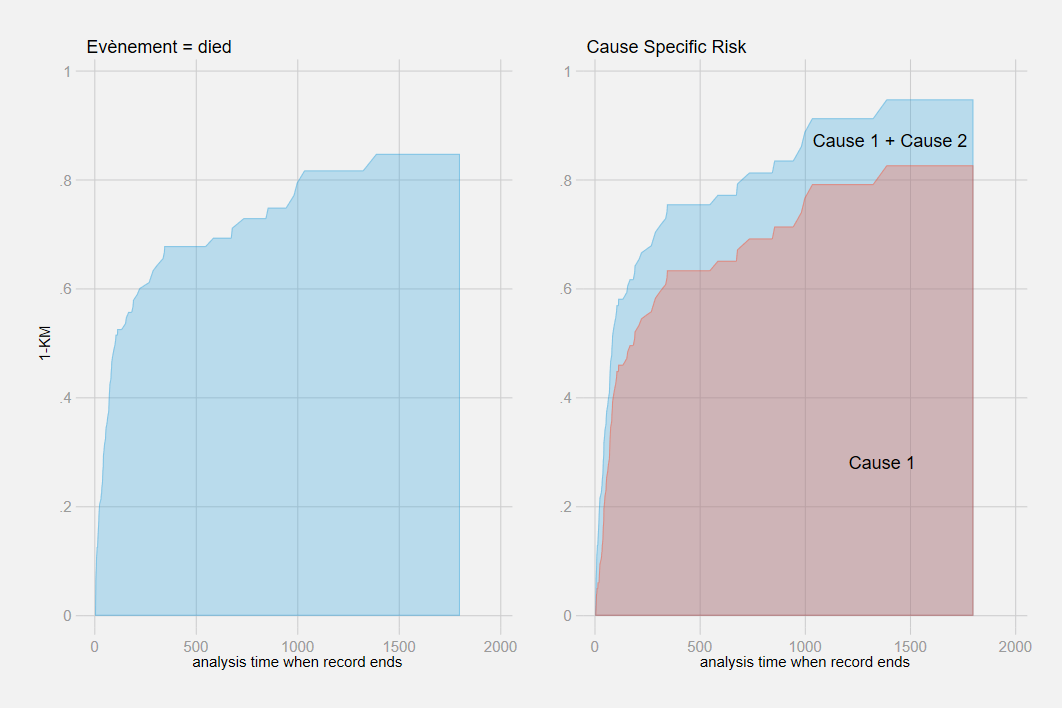
\includegraphics{images/Image16.png}

}

\end{figure}

\hypertarget{estimations-en-pruxe9sence-de-risques-concurrents-cif}{%
\section{\texorpdfstring{\textbf{Estimations en présence de risques
concurrents
(CIF)}}{Estimations en présence de risques concurrents (CIF)}}\label{estimations-en-pruxe9sence-de-risques-concurrents-cif}}

\hypertarget{estimation-non-paramuxe9trique}{%
\subsection{Estimation non
paramétrique}\label{estimation-non-paramuxe9trique}}

\begin{itemize}
\tightlist
\item
  Utiliser l'estimateur de Nelson Aalen: il s'agit du risque instantané
  cumulé. Comme il ne s'agit pas d'une probabilité, il a été longtemps
  utilisé comme mesure de l'incidence en présence de risques concurrents
  dans une logique dite \emph{cause specific}.
\end{itemize}

\[H_k (t_i)=\sum_{t_i\leq t}\left(\frac{e_{i,k}}{n_i}\right) \]

\begin{itemize}
\item
  Actuellement, l'estimateur le plus utilisé est la fonction dite
  d'\textbf{incidence cumulée - CIF-} de Kalbfleisch-Prentice et
  Marubini-Valscchi:

  \begin{itemize}
  \tightlist
  \item
    Il repose sur une probabilité tout en supportant la non indépendance
    des risques.
  \item
    Son interprétation est identique à la fonction de répartition
    \(F(t)=1-S(t)\). Cette fonction est donc croissante.
  \item
    Il est possible de tester les différences entres CIF: \emph{test de
    Gray} (R, SAS) ou \emph{test de Pepe-Mori} (Stata).
  \end{itemize}
\end{itemize}

\textbf{CIF (Cumulative Incidence Function)}

\begin{itemize}
\tightlist
\item
  Si \(h_k(t_i)\) est le risque \emph{cause-spécific} en \(t_i\) et
  \(S(t_i-1)\) l'estimateur de Kaplan-Meier en \(t_i-1\) lorsque tous
  les risques sont regroupés en un évènement unique, l'incidence cumulée
  pour le risque \(k\) en \(t_i\) est égale à:
\end{itemize}

\[IC_k(t_i)= \sum_{t_i\leq t}S(t_i-1)h_k(t_i)\]

\begin{itemize}
\tightlist
\item
  Les valeurs prises par cette fonction pour la cause \(k\) ne dépendent
  donc pas seulement des individus ayant observé l'évènement à partir de
  cette seule cause, mais aussi du nombre de personnes qui n'ont pas
  encore observés l'évènement à partir des autres causes identifiées.
  Cette dernière information est donnée par \(S(t_i-1)\).
\item
  L'incidence cumulée peut ainsi s'interpréter, simplement, comme la
  proportion d'individus qui sont sortis du risque jusqu'en \(t_i\) en
  raison de la cause \(k\).
\end{itemize}

\begin{figure}

\caption{Risques concurrent: estimation de la CIF}

{\centering 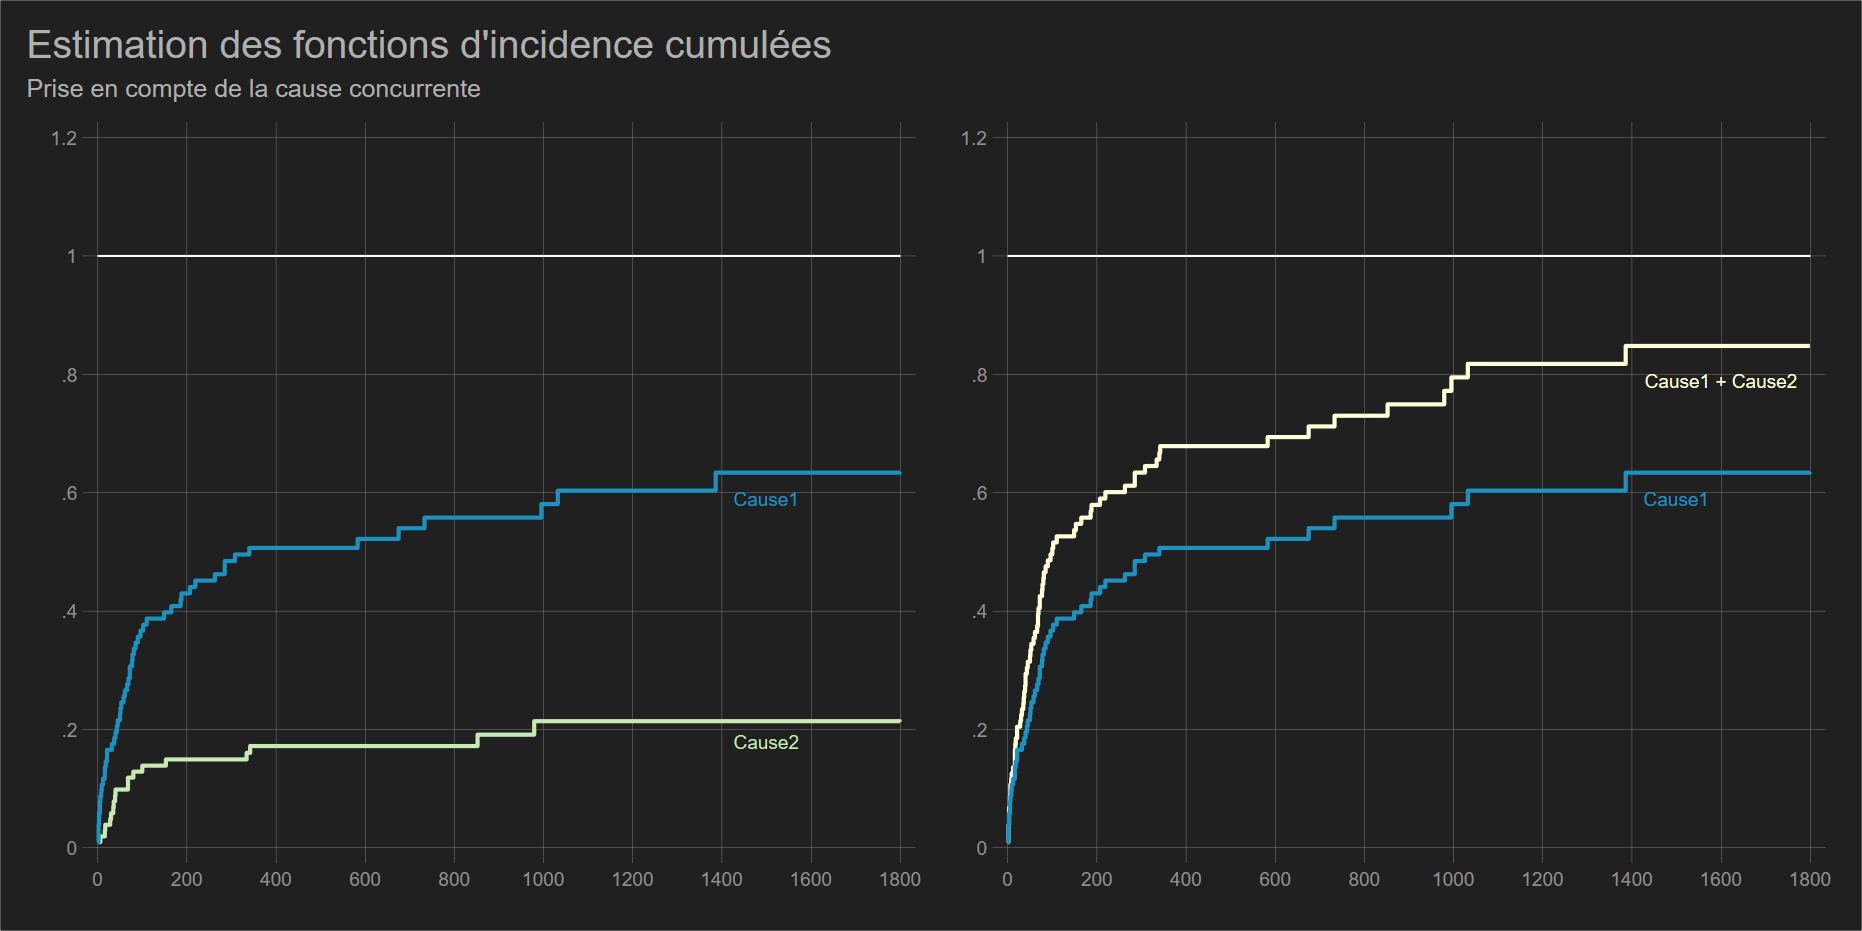
\includegraphics{images/Image17.png}

}

\end{figure}

\begin{verbatim}

            failure:  compet == 1
 competing failures:  compet == 2

    Time       CIF         SE     [95% Conf. Int.]
--------------------------------------------------
\end{verbatim}

\begin{verbatim}
       1    0.0097     0.0097     0.0009    0.0477
       2    0.0388     0.0190     0.0127    0.0892
       3    0.0583     0.0231     0.0239    0.1149
       5    0.0777     0.0264     0.0363    0.1395
       6    0.0874     0.0278     0.0429    0.1515
       8    0.0971     0.0292     0.0497    0.1634
       9    0.1068     0.0304     0.0566    0.1751
      12    0.1166     0.0316     0.0638    0.1868
      16    0.1362     0.0338     0.0785    0.2099
      18    0.1461     0.0349     0.0860    0.2212
      21    0.1657     0.0367     0.1014    0.2437
      32    0.1756     0.0376     0.1093    0.2550
      37    0.1856     0.0384     0.1173    0.2662
      40    0.1957     0.0393     0.1254    0.2775
      43    0.2058     0.0400     0.1337    0.2888
      45    0.2158     0.0408     0.1420    0.2999
      50    0.2259     0.0415     0.1503    0.3110
      51    0.2360     0.0422     0.1588    0.3221
      53    0.2461     0.0428     0.1673    0.3330
      58    0.2562     0.0434     0.1759    0.3439
      61    0.2662     0.0440     0.1845    0.3548
      66    0.2763     0.0445     0.1932    0.3656
      69    0.2864     0.0450     0.2020    0.3763
      72    0.3066     0.0459     0.2197    0.3976
      77    0.3167     0.0464     0.2286    0.4082
      78    0.3267     0.0467     0.2376    0.4187
      81    0.3368     0.0471     0.2466    0.4292
      85    0.3469     0.0475     0.2556    0.4396
      90    0.3570     0.0478     0.2648    0.4500
      96    0.3671     0.0481     0.2739    0.4604
     102    0.3771     0.0484     0.2831    0.4707
     110    0.3874     0.0487     0.2925    0.4812
     149    0.3980     0.0489     0.3021    0.4920
     165    0.4085     0.0492     0.3118    0.5027
     186    0.4193     0.0495     0.3217    0.5137
     188    0.4301     0.0497     0.3316    0.5246
     207    0.4408     0.0499     0.3417    0.5354
     219    0.4516     0.0501     0.3517    0.5462
     263    0.4624     0.0502     0.3618    0.5570
     285    0.4846     0.0505     0.3826    0.5791
     308    0.4957     0.0506     0.3931    0.5900
     340    0.5068     0.0507     0.4037    0.6009
     583    0.5221     0.0514     0.4171    0.6168
     675    0.5401     0.0524     0.4322    0.6361
     733    0.5580     0.0532     0.4477    0.6548
     995    0.5808     0.0548     0.4659    0.6795
    1032    0.6036     0.0559     0.4851    0.7031
    1386    0.6340     0.0583     0.5083    0.7357


            failure:  compet == 2
 competing failures:  compet == 1

    Time       CIF         SE     [95% Conf. Int.]
--------------------------------------------------
       3    0.0097     0.0097     0.0009    0.0477
       6    0.0194     0.0136     0.0038    0.0619
      16    0.0292     0.0166     0.0079    0.0761
      17    0.0391     0.0191     0.0128    0.0897
      28    0.0489     0.0213     0.0182    0.1029
      30    0.0587     0.0232     0.0240    0.1157
      35    0.0686     0.0250     0.0302    0.1286
      36    0.0786     0.0267     0.0367    0.1411
      39    0.0885     0.0282     0.0435    0.1534
      40    0.0986     0.0296     0.0504    0.1658
      68    0.1188     0.0322     0.0650    0.1901
      80    0.1288     0.0334     0.0724    0.2020
     100    0.1389     0.0345     0.0800    0.2138
     153    0.1495     0.0356     0.0880    0.2261
     334    0.1605     0.0368     0.0964    0.2392
     342    0.1720     0.0381     0.1052    0.2526
     852    0.1913     0.0417     0.1175    0.2787
     979    0.2141     0.0460     0.1320    0.3094
\end{verbatim}

En présence du risque concurrent, et traité comme tel, la moitié des
personnes sont décédées suite à la malformation cardiaque au bout de 308
jours (200 jours avec une estimation de type « cause specific »).

On peut vérifier que la somme des estimateurs permet d'obtenir la survie
\emph{toutes causes confondues}. Il n'y a pas de surprise à cela, dans
l'estimateur Marubini-Valscchi la survie d'ensemble intervient comme un
facteur de pondération du quotient d'intensité dite « cause-specific ».

\begin{tcolorbox}[enhanced jigsaw, arc=.35mm, bottomrule=.15mm, titlerule=0mm, colbacktitle=quarto-callout-tip-color!10!white, left=2mm, opacitybacktitle=0.6, toprule=.15mm, title=\textcolor{quarto-callout-tip-color}{\faLightbulb}\hspace{0.5em}{\textbf{R-Stata-Sas-Python}}, colframe=quarto-callout-tip-color-frame, breakable, coltitle=black, opacityback=0, toptitle=1mm, bottomtitle=1mm, rightrule=.15mm, leftrule=.75mm, colback=white]

L'estimation avec des risques de type « cause-specific » demande juste
de recoder la variable évènement/censure, en glissant les risques
concurrents en censure à droite.

Pour l'estimation des CIF (risque de sous répartition):

\begin{itemize}
\item
  \textbf{R}: la librairie \textbf{\texttt{cmprsk}} permet d'estimer
  simplement les incidences cumulées avec la fonction
  \textbf{\texttt{cuminc}}.
\item
  \textbf{Sas}: maintenant directement estimable avec
  \texttt{proc\ lifetest}. Il suffit d'indiquer le ou les risques
  d'intérêt dans l'instruction indiquant la variable de durée et de
  censure avec l'option \textbf{\texttt{failcode=valeur}}.
\item
  \textbf{Stata}: Estimation avec la commande externe
  \textbf{\texttt{stcompet}}. La commande génère des variables qui
  demande des manipulations supplémentaires pour afficher les résultats
  sous forme de tableau par exemple. On peut utiliser et préférer la
  commande externe \textbf{\texttt{stcomlist}}.
\item
  \textbf{Python}: le wrapper de R (\texttt{cmprsk}) ne fonctionne plus
  à ce jour à défaut de mise à jour {[}2022{]}.
\end{itemize}

\end{tcolorbox}

\hypertarget{compararaison-des-cif}{%
\subsection{Compararaison des CIF}\label{compararaison-des-cif}}

\begin{itemize}
\item
  \textbf{Test d'homogénéité de Gray}: est basé sur une autre mesure du
  risque en évènement concurrent. Sur le principe, identique à la
  philosopjie des test du logrank. Il s'agit du « subdistribution risks
  (« risque de sous-répartition », A.Latouche). Son interprétation n'est
  pas aisée car les personnes ayant observé un risque concurrent sont
  remises dans le Risk Set. Mais il est directement lié à l'estimation
  des CIF. Disponible avec SAS et R. Il est également sensible
  l'hypothèse de proportionnalité et à la distribution des censures à
  droites entre les groupes comparés. A ma connaissance il n'y a pas de
  variantes pondérées.
\item
  \textbf{Test de Pepe \& Mori}: teste directement deux courbes
  d'incidences et seulement 2. Je n'ai pas le recul nécessaire sur cette
  alternative, qui n'est implémenté que dans Stata.
\end{itemize}

\begin{longtable}[]{@{}lll@{}}
\caption{Test de Gray pour la variable surgery}\tabularnewline
\toprule\noalign{}
Risques & Chi2 & P\textgreater Chi2 \\
\midrule\noalign{}
\endfirsthead
\toprule\noalign{}
Risques & Chi2 & P\textgreater Chi2 \\
\midrule\noalign{}
\endhead
\bottomrule\noalign{}
\endlastfoot
Cause1 & 5.783 & 0.0161 \\
Cause2 & 0.129 & 0.7191 \\
\end{longtable}

\begin{longtable}[]{@{}lll@{}}
\caption{Test de Pepe-Mori pour la variable surgery}\tabularnewline
\toprule\noalign{}
Risques & Chi2 & P\textgreater Chi2 \\
\midrule\noalign{}
\endfirsthead
\toprule\noalign{}
Risques & Chi2 & P\textgreater Chi2 \\
\midrule\noalign{}
\endhead
\bottomrule\noalign{}
\endlastfoot
Cause1 & 6.203 & 0.0127 \\
Cause2 & 1.880 & 0.7038 \\
\end{longtable}

\begin{tcolorbox}[enhanced jigsaw, arc=.35mm, bottomrule=.15mm, titlerule=0mm, colbacktitle=quarto-callout-tip-color!10!white, left=2mm, opacitybacktitle=0.6, toprule=.15mm, title=\textcolor{quarto-callout-tip-color}{\faLightbulb}\hspace{0.5em}{\textbf{R-Stata-Sas-Python}}, colframe=quarto-callout-tip-color-frame, breakable, coltitle=black, opacityback=0, toptitle=1mm, bottomtitle=1mm, rightrule=.15mm, leftrule=.75mm, colback=white]

\begin{itemize}
\item
  \textbf{Sas}: le test de Gray est estimé si on ajoute l'option
  strata=nom\_variable à la proc lifetest sous risque concurrent (voir
  encadré précédent). Le test de Pepe-Mori est disponible via une macro
  externe (\texttt{\%compcif}: non testée) :
\item
  \textbf{Stata}: Le test de Gray n'est pas disponible, il faut passer
  par une exécution de la fonction cuminc de la librairie R cmprsk
  directement dans stata (voir la commande \texttt{rsource}). Pour faire
  plus simple, on peut estimer le modèle de Fine-Gray avec une seule
  variable (discrète). Le résultat est comparable à celui du test (voir
  plus bas). Le test de Pepe-Mori est disponible via la commande externe
  \texttt{stpepemori}.
\item
  \textbf{R}: On ajoute une variable à la fonction \texttt{cuminc} de la
  librairie \textbf{\texttt{cmprsk}}. Pas de test de \emph{Pepe-Mori}
  sur les fonctions d'incidence à ma connaissance.
\item
  \textbf{Python}: ne pas essayer d'utiliser la librairie cmprsk qui
  n'est pas mis à jour et ne fonctionne plus.
\end{itemize}

\end{tcolorbox}

\hypertarget{moduxe8les}{%
\section{\texorpdfstring{\textbf{Modèles}}{Modèles}}\label{moduxe8les}}

\hypertarget{moduxe8les-semi-paramuxe9triques}{%
\subsection{Modèles Semi
paramétriques}\label{moduxe8les-semi-paramuxe9triques}}

Cette présentation sera plutôt brève. Dans le domaine des sciences
sociales, je préconise plutôt l'utilisation d'un modèle multinomial à
temps discret de type logistique. Le modèle de Cox en présence de
risques concurrent n'est valable que dans une logique de risques «
cause-specific », le modèle de Fine et Gray bien que directement relié à
l'estimation des incidences cumulées, repose sur une définition du
risque (de sous répartition) dont l'interprétation n'est pas naturelle.
Il est également soumis à l'hypothèse de proportionnalité des risques.

\textbf{Modélisation des risques « cause-specific » : Cox}\\
Modèle de Cox «standard» pour chaque évènement, les évènements
concurrents sont traités comme des censures à droite. Aucune
interprétation sur les fonctions d'incidence ne peut-être faite.

\textbf{Modèle de Fine-Gray: subdistribution hazard regression}\\
Modèle de type semi-paramétrique avec une redéfinition du risque lié à
l'estimation des fonctions d'incidence (voir test de Gray). La
différence avec le Cox classique réside dans le calcul du risk-set : les
évènements concurrents ne sont pas considérés comme des censures, on
laisse les individus leur « survivre » jusqu'à la durée maximale
observée dans l'échantillon. L'interprétation n'est donc pas très
intuitive (Fine et Gray le soulignent). Ce modèle est relativement
contreversé. Il ne sera donc pas exécuté pour l'application

Pour les questions liées à l'interprétation de ces deux types de
modèles, se reporter à:
\url{https://onlinelibrary.wiley.com/doi/epdf/10.1002/sim.7501}

\begin{tcolorbox}[enhanced jigsaw, arc=.35mm, bottomrule=.15mm, titlerule=0mm, colbacktitle=quarto-callout-tip-color!10!white, left=2mm, opacitybacktitle=0.6, toprule=.15mm, title=\textcolor{quarto-callout-tip-color}{\faLightbulb}\hspace{0.5em}{R-Stata-Sas-Python}, colframe=quarto-callout-tip-color-frame, breakable, coltitle=black, opacityback=0, toptitle=1mm, bottomtitle=1mm, rightrule=.15mm, leftrule=.75mm, colback=white]

\begin{itemize}
\item
  \textbf{R}: on utilise la fonction \textbf{\texttt{crr}} du package
  cmprsk.
\item
  \textbf{Sas}: même principe que pour l'estimation non paramétrique, on
  ajoute l'option \texttt{eventcode=valeur} à l'instruction
  \texttt{model} de la \texttt{proc\ phreg}.
\item
  \textbf{Stata}: on utilise la commande interne
  \textbf{\texttt{stcrreg}}.
\item
  \textbf{Python} : ne pas essayer d'utiliser la librairie cmprsk qui
  n'est pas mis à jour et ne fonctionne donc plus.
\end{itemize}

\end{tcolorbox}

\hypertarget{moduxe8le-uxe0-temps-discret-1}{%
\subsection{Modèle à temps
discret}\label{moduxe8le-uxe0-temps-discret-1}}

\begin{itemize}
\item
  Il s'agit d'une extension du modèle à temps discret à évènement unique
  (toutes causes regroupées) avec ici le modèle logistique multinomial.
\item
  S'il ne permet pas une interprétation sur les fonctions d'incidences,
  les risques concurrents ne sont pas traitées comme des censures à
  droite.
\item
  Le modèle multinomial repose sur une hypothèse dite « d'indépendance
  des alternatives non pertinentes » (IIA). Cela peut donc paraitre
  contradictoire d'utiliser ce modèle pour des évènements qui sont
  supposés non indépendants. Néanmoins la dépendance entre risques
  concurrents n'est pas non plus stricte et cette hypothèse d'IIA,
  seulement testable par le bon sens, est souvent illustrée par
  l'exemple des couleurs des bus dans le choix du mode de transport, ou
  les couleurs de chaussure dans les études marketing. Soit est une
  situation relativement limite.
\item
  En terme de lecture, les estiupateurs du modèle logistique multinomial
  peuvent directement s'interpréter comme des rapports de risque (ou
  relative risk ratio).
\item
  En sciences sociales, il me semble que ce type de modèle soit à
  privilégier.
\item
  On peut également envisager un modèle de type probit multinomial, mais
  on peut rencontrer des problèmes d'estimations (repose sur la loi
  normale multivariée). Prévoir un regroupement des causes concurrentes,
  et dans tous les cas de figure ne pas dépasser trois causes.
\item
  Niveau lecture, on peut utiliser une méthode de standardisation, de
  type \textbf{AME} (\emph{Average Marginal Effect}).
\end{itemize}

Pour l'application, nous avons pris le mois (30 jours) comme métrique
temporelle. On rappelle que les valeurs des estimateurs sont fictives en
raison de la simulation des évènement pour le risque concurrent (cause2)

\begin{table}

\caption{\label{tbl-panel}Modèle logistique multinomial avec risques
concurrent}\begin{minipage}[t]{0.50\linewidth}
\subcaption{\label{tbl-first}Cause 1}

{\centering 

\begin{tabular}[t]{llll}
\toprule
Cause 1 & RRR & p\textgreater\textbar z\textbar{} & 95\% IC\\
\midrule
\(t\) & 0.816 & 0.000 & 0.752 - 0.885\\
\(t^2\) & 1.003 & 0.000 & 1.001 - 1.005\\
\(year\) & 0.879 & 0.116 & 0.749 - 1.032\\
\(age\) & 1.045 & 0.012 & 1.010 - 1.081\\
\(surgery\) & 0.318 & 0.033 & 0.110 - 0.913\\
\(constante\) & 0.231 & 0.000 & 0.148 - 0.360\\
\bottomrule
\end{tabular}

}

\end{minipage}%
%
\begin{minipage}[t]{0.50\linewidth}
\subcaption{\label{tbl-second}Cause 2}

{\centering 

\begin{tabular}[t]{llll}
\toprule
Cause 2 & RRR & p\textgreater\textbar z\textbar{} & 95\% IC\\
\midrule
\(t\) & 0.817 & 0.003 & 0.713 - 0.935\\
\(t^2\) & 1.003 & 0.052 & 1.000 - 1.006\\
\(year\) & 0.816 & 0.141 & 0.622 - 1.070\\
\(age\) & 1.011 & 0.654 & 0.964 - 1.061\\
\(surgery\) & 0.541 & 0.431 & 0.117 - 2.496\\
\(constante\) & 0.076 & 0.000 & 0.037 - 0.157\\
\bottomrule
\end{tabular}

}

\end{minipage}%

\end{table}

Notes:

\begin{itemize}
\tightlist
\item
  On a utilisé le terme RRR - Relative Risk Ratio - pour la colonne
  raportant les estimations. Dans un cadre de risque concurrent il est
  un peu difficile d'utiliser formellement la notion de \emph{hazard
  rate} tel qu'il a été difini plus haut, enfin les modèles multinomiaux
  ne reportent pas formellement des Odds Ratios dont l'utilisation
  devrait être réservé exclusivement à une alternative binaire.
\item
  les variables \emph{year} et \emph{age} ont été centrées sur leur
  valeur moyenne pour donner aux constantes des valeurs acceptables.
\item
  Pour faciliter la lecture on peut utiliser une méthode de
  standardisation de type AME (Average Marginal Effect).
\end{itemize}

\hypertarget{moduxe8les-paramuxe9triques}{%
\chapter{\texorpdfstring{\textbf{Modèles
paramétriques}}{Modèles paramétriques}}\label{moduxe8les-paramuxe9triques}}

\textbf{Objectifs}: présenter, assez rapidement, la logique des modèles
de type \textbf{AFT} (\textbf{Accelerated Failure Time}), principalement
celui de \emph{Weibull}.

\hypertarget{principes}{%
\section{Principes}\label{principes}}

\begin{itemize}
\tightlist
\item
  Dans les modèles paramétriques usuels, la durée de survie est
  distribuée selon une loi dont la densité \(f(t)\) pleinement
  paramétrée.\\
\item
  Pour utiliser l'approche paramétrique, il faut avoir de bonnes raisons
  de penser que durée de survie sont distribués selon une certaine loi
  connue plutôt qu'une autre.
\item
  La majorité des distributions reposent sur une hypothèse dite AFT
  (\textbf{Acceleretad Failure Time}). Une autre, \emph{Gompertz}, très
  utilisée en démographie (mortalité), repose seulement sur la
  proportionnalité des risques. Certaines peuvent reposer sur les deux
  comme le modèle de \emph{Weibull}. Enfin, les modèles
  \emph{log-logistique} ou \emph{log-normal} n'ont qu'une
  paramétrisation de type \emph{AFT}.
\end{itemize}

\hypertarget{hypothuxe8se-aft-accelerated-failure-time}{%
\section{Hypothèse AFT: Accelerated Failure
Time}\label{hypothuxe8se-aft-accelerated-failure-time}}

L'hypothèse \textbf{AFT} signifie que l'effet des covariables est
multiplicatif par rapport à la durée de survie/séjour. Par opposition,
les modèles PH décrivent un effet multiplicatif par rapport au risque.

Selon les caractérisques des individus, le temps \emph{ne s'écoulent pas
à la même vitesse}, ils ne partagent donc plus la même métrique
temporelle. Cela renvoie a des interprétations de type
\emph{dilation/contraction} du temps, par analogie à la théorie de la
relativité.

Exemple simple: la durée de vie d'un être humain et d'un chien.\\
On dit qu'une année de vie d'un être humain est équivalent à 7 années de
vie d'un chien. C'est typiquement une hypothèse d'AFT.\\
\(S_h(t) = S_c(7\times t)\).

C'est ce facteur multiplicatif qu'estime un modèle paramétrique de type
AFT.

\[S(t_i | X_1)=  S(\phi t_i | X_0)\]

Remarque: si un modèle s'estime AFT s'estime également sous hypothèse PH
comme celui de Weibull: \(h(t_i | X_1)= -\rho \phi h(t_i | X_0)\)

\begin{itemize}
\tightlist
\item
  Avantage: l'interprétation des modèles est directement liée aux
  fonctions de survie. Cela s'avère donc pratique après une analyse non
  paramétrique de type Kaplan-Meier par exemple.
\item
  Inconvénient: ne permet pas l'introduction de variables dynamiques.
\end{itemize}

\emph{Humain versus chien}: la probabilité qu'un être humain survive 80
ans est égale à la probabilité qu'un chien survive 11 ans (80/7). Le
temps s'écoulerait donc plus vite pour le chien que pour l'être humain
du point de vue d'un référentiel extérieur. Ce raisonnement peut
s'appliquer aux quantile du temps de survie: le temps de survie médian
d'un être humain est 7 fois plus élevé que celui d'un chien. En terme
d'interprétation des paramètres estimés, si la durée de survie est plus
courte, alors le risque est plus élevé.

\hypertarget{principe-de-construction-des-moduxe8les-aft}{%
\section{Principe de construction des modèles
AFT}\label{principe-de-construction-des-moduxe8les-aft}}

Le raisonnement mathématique est ici plus complexe que pour les modèles
de Cox ou à durée discrète. On donnera juste quelques pistes en début de
raisonnement. On part d'une expression proche du modèle linéaire à une
transformation logarithmique près de la variable dépendante. En imposant
la contrainte \(t_i>0\), en ne posant qu'une seule covariable \(X\) de
type binaire, et en se situant de nouveau dans une logique de temps
continu (pas d'évènement simultané):

\[log(t_i)= \alpha_0 +  \alpha_1X_i + bu_i\]

\(b\) est un paramètre d'échelle identique pour toutes les observations
et \(u_i\) un terme terme d'erreur qui suit une loi de distribution de
densité \(f(u)\). Cette combinaison linéaire définira le paramètre de
position. C'est la forme de \(f(u)\) qui définie le type de modèle
paramétrique.

On peut écrire:
\(f(u_i) = f(\frac{log(t_i)- \alpha_0 - \alpha_1X_i}{b})\).

Remarque: pour une distibution normale/gaussienne, le paramètre de
position est l'espérance et le paramètre d'échelle l'écart-type.

\hypertarget{quelques-moduxe8les-paramuxe9triques-usuels}{%
\section{Quelques modèles paramétriques
usuels}\label{quelques-moduxe8les-paramuxe9triques-usuels}}

\textbf{Modèle exponentiel et de Weibull}

\textbf{Weibull}

\begin{itemize}
\tightlist
\item
  Peut estimer un modèle PH ou AFT, d'où sa popularité.
\item
  Distribution monotone des durées d'évènement, toujours croissante ou
  décroissante.
\item
  \(f(t)=\lambda\alpha t^{\alpha - 1}e^{-\alpha t^\lambda}\) et
  \(h(t)=\lambda\alpha(\lambda t)^{\alpha - 1}\), \(\alpha>0\) et
  \(\lambda>0\). Si \(\lambda>1\) le risque est croissant, décroissant
  si \(\lambda<1\), et est constant (loi exponentielle) si
  \(\lambda=1\).
\end{itemize}

\emph{Exponentiel}

\begin{itemize}
\tightlist
\item
  Processus sans mémoire, utilisé pour étudier par exemple la durée de
  vie composants électriques ou électroniques.
\item
  La fonction de risque est une constante.
\item
  Cas limite de la loi de Weibull. Un modèle de type exponentiel
  peut-être de type AFT ou PH.
\item
  Pour contourner la constance du risque dans le temps, on peut estimer
  un modèle en scindant la durée en plusieurs intervalles. Le risque
  sera constant à l'intérieur de ces intervalles, il s'agit d'un modèle
  ``exponential piecewise'' (exponentiel par morceau).
\end{itemize}

\textbf{Log-logistique}

\begin{itemize}
\tightlist
\item
  Estime un modèle de type AFT seulement. Proche du modèle log-normal
  (plus difficile à estimer).
\item
  Permet une interprétation en terme d'Odds de survie.
\item
  La fontion du risque peut-être ``U-shaped'' (unimodale croissante puis
  décroissante).
\end{itemize}

\textbf{Autres lois}: Gompertz (PH seulement), Gamma et Gamma
généralisé\ldots..

\textbf{Sélection de la loi} On peut sélectionner la loi en comprarant
les AIC où les BIC des modèles. Pour le modèle de Weibull, on peut
regarder s'il ajuste bien les données si la transformation
\(log(-log(S(t_i)))\) est linéaire par rapport à \(log(t_i)\).

\textbf{\emph{Application}}

\textbf{\emph{Comparaison des AIC (sans covariable)}}

\begin{itemize}
\tightlist
\item
  Weibull: 400.1\\
\item
  Exponentiel: 461.0\\
\item
  Gompertz: 409.6\\
\item
  Log-logistique: 391.8
\end{itemize}

\hypertarget{exemple-avec-le-moduxe8le-de-weibull}{%
\section{Exemple avec le modèle de
Weibull}\label{exemple-avec-le-moduxe8le-de-weibull}}

\begin{table}

\caption{\label{tbl-panel}Modèle de
Weibull}\begin{minipage}[t]{0.50\linewidth}
\subcaption{\label{tbl-first}Accelerated Failure Time (AFT)}

{\centering 

\begin{tabular}[t]{llll}
\toprule
Variables & Time Ratio & p\textgreater\textbar z\textbar{} & 95\% IC\\
\midrule
\(year\) & 1.176 & 0.184 & 0.926 - 1.493\\
\(age\) & 0.940 & 0.013 & 0.896 - 0.987\\
\(surgery\) & 7.173 & 0.011 & 1.557 - 33.048\\
\(\rho\) & 0.556 & - & 0.464 - 0.667\\
\bottomrule
\end{tabular}

}

\end{minipage}%
%
\begin{minipage}[t]{0.50\linewidth}
\subcaption{\label{tbl-second}Proportional hazard (PH)}

{\centering 

\begin{tabular}[t]{llll}
\toprule
Variables & HR & p\textgreater\textbar z\textbar{} & 95\% IC\\
\midrule
\(year\) & 0.914 & 0.175 & 0.802 - 1.041\\
\(age\) & 1.035 & 0.014 & 1.007 - 1.063\\
\(surgery\) & 0.334 & 0.012 & 0.143 - 0.783\\
\(\rho\) & 0.556 & - & 0.464 - 0.667\\
\bottomrule
\end{tabular}

}

\end{minipage}%

\end{table}

Note: la constante n'est pas reporté. \(\rho\) indique la valeur estimé
d'un paramètre de \emph{forme}. Son signe indique sur le risque est
décroissant ou croissant (1 si risque constant), et permet de passer de
la paramétrisation AFT à la paramétrisation PH (et inversement).

\begin{itemize}
\item
  \textbf{AFT}: Un jour de survie d'une personne qui n'a pas été opérée
  d'un pontage correspond environ à 7 jours de survie d'une personne
  opérée. Cette remise à l'échelle de la métrique temporelle entre les
  deux groupes exprime bien le gain en durée de survie pour les
  personnes opérées, soit des risques journaliers de décès plus faibles
  (et plus faibles à valeurs constantes, proportionnalité oblige).
\item
  \textbf{PH}: Lecture en rapport de risque ou \emph{hazard rate} (idem
  Cox). Si on avait reporté les coefficients (échelle log)
  \(b_{ph} = -\rho \times b_{aft}\). Ici
  \(-0.556 \times (1.97) = -1.096\). Et \(e^{-1.096}=0.334\)
\end{itemize}

Attention: on ne peut pas comparer la qualité d'un modèle paramétrique à
celle d'un modèle de Cox par des critères type AIC ou BIC. Les deux
méthodes d'estimation diffèrent.

\hypertarget{le-moduxe8le-de-parmar-royston}{%
\section{Le modèle de
Parmar-Royston}\label{le-moduxe8le-de-parmar-royston}}

\begin{itemize}
\tightlist
\item
  Le bon ajustement par une loi de distribution predéfinie peut s'avérer
  contraignante. Le modèle de Cox avait justement pour objectif de se
  défaire de cette contrainte, la plupart des distributions utilisée
  étant monotone ou unimodale (log-logistique ou log-normal).
\item
  Le principe des splines peut-être rapproché de celui qui a été utilisé
  plus haut dans le modèle logistique à durée discrète avec
  l'introduction des polynomes {[}
  \(f(t)= (a_1\times t) + (a_2\times t^2) + (a_3\times t^3) + ...+ (a_k\times t^k)\).

  \begin{itemize}
  \tightlist
  \item
    Cette méthode brute d'ajustement consiste finalement à introduire
    une intéraction ou plusieurs intéractions entre la variable de durée
    avec elle-même.
  \item
    Elle est sujette à une forte sensibilité aux outliers (overfitting)
    au delà de \(k>2\) {[}lors la formation il suffit de la tester pour
    k=3 et calculer la probabilité conditionnelle pour s'en
    convaincre{]}.
  \end{itemize}
\item
  Les \textbf{splines cubiques restreintes} propose une méthode
  d'ajustement et de lissage de meilleure qualité et permet de contrôler
  les effets overfitting.

  \begin{itemize}
  \tightlist
  \item
    les splines cubiques sont donc basées sur des polynomes d'ordre 3
    (d'où cubique) avec une estimation par morceau (intervalles). les
    morceaux sont définis manuellement ou par un nombre de degrés de
    liberté obtenu par quantile du logarithme de la fonction de survie
    après avoir exclu les observation censurées.

    \begin{itemize}
    \tightlist
    \item
      Deux degrés de liberté (1 noeud) avec un intervalle allant
      jusqu'au log de la moitié des survivants et un second à partir de
      cette seconde moitié.
    \item
      Sur le même principe trois degrés de liberté (2 noeuds) coupe la
      durée en 3 intervalles sur ses terciles.
    \item
      En pratique, il est préférable de donner à l'application de nombre
      de degré de liberté plutôt que d'indiquer manuellement la position
      des noeuds.
    \item
      Il convient également de ne pas être trop gourmand sur le nombre
      de noeuds, un ou deux étant souvant suffisant (donc 2 ou 3 degrés
      de liberté).
    \item
      On peut choisir le nombre de degrés de liberté en estimant des
      modèles sans covariables et comparer les AIC (vraisemblance
      pénalisée).
    \end{itemize}
  \end{itemize}
\item
  Contrairement aux autres modèles, et sans rentrer dans les détails, le
  modèle de Parmar-Royston part de la fonction de risque cumulée et non
  des taux de risque/hasard. Les risk ratios sont obtenus en utilisant
  les relations entre les différentes grandeurs (voir section *théorie).
\end{itemize}

\textbf{Exemple}

Avec 2 degrés de liberté (un noeud):

\begin{longtable}[]{@{}llll@{}}
\caption{Modèle de Parmar-Roytston}\tabularnewline
\toprule\noalign{}
Variables & \$e\^{}(b) & p\textgreater\textbar z\textbar{} & 95\% IC \\
\midrule\noalign{}
\endfirsthead
\toprule\noalign{}
Variables & \$e\^{}(b) & p\textgreater\textbar z\textbar{} & 95\% IC \\
\midrule\noalign{}
\endhead
\bottomrule\noalign{}
\endlastfoot
\(year\) & 0.885 & 0.067 & 0.777 - 1.008 \\
\(age\) & 1.030 & 0.026 & 1.004 - 1.058 \\
\(surgery\) & 0.373 & 0.025 & 0.159 - 0.876 \\
\(spline 1\) & 3.157 & 0.000 & 2.503 - 3.981 \\
\(spline 2\) & 1.289 & 0.002 & 1.099 - 1.511 \\
\(constante\) & 0.510 & 0.000 & 0.386 - 0.674 \\
\end{longtable}

A savoir:

\begin{itemize}
\tightlist
\item
  Avec un degré de liberté, le modèle de Parmar-Royston estime un modèle
  de Weibull sous paramétrisation PH.
\item
  Les paramètres pour les splines ne sont pas interprétables
  directement. Ils servent calculer la baseline du risque via l'équation
  du polynome (non reporté car expression bien corsée).
\end{itemize}

\hypertarget{annexes}{%
\chapter{\texorpdfstring{\textbf{Annexes}}{Annexes}}\label{annexes}}

\hypertarget{tests-grambsch-therneau-ols-sur-les-ruxe9sidus-de-schoenfeld}{%
\section{Tests Grambsch-Therneau OLS sur les résidus de
Schoenfeld}\label{tests-grambsch-therneau-ols-sur-les-ruxe9sidus-de-schoenfeld}}

\begin{tcolorbox}[enhanced jigsaw, arc=.35mm, bottomrule=.15mm, titlerule=0mm, colbacktitle=quarto-callout-important-color!10!white, left=2mm, opacitybacktitle=0.6, toprule=.15mm, title=\textcolor{quarto-callout-important-color}{\faExclamation}\hspace{0.5em}{Important}, colframe=quarto-callout-important-color-frame, breakable, coltitle=black, opacityback=0, toptitle=1mm, bottomtitle=1mm, rightrule=.15mm, leftrule=.75mm, colback=white]

Attention il ne s'agit pas du test actuellement implémenté dans la
nouvelle version de \texttt{survival} (v3) qui, malheureusement, lui a
substitué la version dite \emph{exacte} (moindres carrés généralisés).
Le programme de la fonction du test OLS est néanmoins facilement
récupérable et exécutable.
\href{https://github.com/mthevenin/analyse_duree/blob/main/cox.zphold/cox.zphold.R}{lien}.

Je continue de préconiser l'utilisation de cette version OLS du test,
reproductible avec les autres applications statistiques
(Stata,Sas,Python).

\end{tcolorbox}

\begin{itemize}
\tightlist
\item
  Le test dit ``simplifié'', qui n'apparait pas dans le texte original
  de P.Gramsch et T.Thernau
  \href{https://www.jstor.org/stable/2337123\#metadata_info_tab_contents}{lien},
  répond à un soucis d'instabilité des variances des résidus de
  Schoenfeld en fin de durée d'observation lorsque peu d'observation
  restent soumises au risque. Cet argument est soulevé dans leur ouvrage
  de 2022
  \href{https://link.springer.com/book/10.1007/978-1-4757-3294-8}{lien}
  avant d'en présenter sa version.
\item
  Il est simplifié car on applique à tous les résidus bruts la variance
  du paramètre (\(b\)) estimés par le modèle de Cox.
\item
  Le test devient alors un simple test de corrélation entre les résidus
  et une fonction de la durée (centrée). Dans l'esprit, il peut être
  également approché par une regression linéaire par les moindre carrés
  ordinaires entre les résidus et une fonction de la durée (voir page
  134 de l'ouvrage de Grambsch et Therneau).
\end{itemize}

Soit les données suivantes, avec \emph{t} la variable de durées,
\emph{Y} la variable de censure et \emph{X} la seule et unique
covariable.

\begin{itemize}
\tightlist
\item
  Pas d'évènement simultané (donc pas de correction de la vraisemblance)
\item
  Covariable de type indicatrice
\end{itemize}

\begin{longtable}[]{@{}lll@{}}
\toprule\noalign{}
\(t_i\) & \(Y_i\) & \(X_i\) \\
\midrule\noalign{}
\endhead
\bottomrule\noalign{}
\endlastfoot
1 & 1 & 1 \\
2 & 0 & 0 \\
3 & 0 & 0 \\
4 & 1 & 1 \\
5 & 1 & 1 \\
6 & 1 & 0 \\
7 & 0 & 1 \\
\end{longtable}

\begin{Shaded}
\begin{Highlighting}[]
\NormalTok{test }\OtherTok{=} \FunctionTok{data.frame}\NormalTok{(}\AttributeTok{time=}  \FunctionTok{c}\NormalTok{(}\DecValTok{1}\NormalTok{,}\DecValTok{2}\NormalTok{,}\DecValTok{3}\NormalTok{,}\DecValTok{4}\NormalTok{,}\DecValTok{5}\NormalTok{,}\DecValTok{6}\NormalTok{,}\DecValTok{7}\NormalTok{),}
                    \AttributeTok{Y=}\FunctionTok{c}\NormalTok{(}\DecValTok{1}\NormalTok{,}\DecValTok{0}\NormalTok{,}\DecValTok{0}\NormalTok{,}\DecValTok{1}\NormalTok{,}\DecValTok{1}\NormalTok{,}\DecValTok{1}\NormalTok{,}\DecValTok{0}\NormalTok{),}
                    \AttributeTok{X=}     \FunctionTok{c}\NormalTok{(}\DecValTok{1}\NormalTok{,}\DecValTok{0}\NormalTok{,}\DecValTok{0}\NormalTok{,}\DecValTok{1}\NormalTok{,}\DecValTok{1}\NormalTok{,}\DecValTok{0}\NormalTok{,}\DecValTok{1}\NormalTok{))}
\end{Highlighting}
\end{Shaded}

Estimation du modèle de Cox:

\begin{Shaded}
\begin{Highlighting}[]
\FunctionTok{library}\NormalTok{(survival)}
\NormalTok{fit }\OtherTok{=} \FunctionTok{coxph}\NormalTok{(}\AttributeTok{formula =} \FunctionTok{Surv}\NormalTok{(time, Y) }\SpecialCharTok{\textasciitilde{}}\NormalTok{ X, }\AttributeTok{data=}\NormalTok{test)}
\NormalTok{fit}
\end{Highlighting}
\end{Shaded}

\begin{verbatim}
Call:
coxph(formula = Surv(time, Y) ~ X, data = test)

    coef exp(coef) se(coef)    z     p
X 0.6217    1.8622   1.1723 0.53 0.596

Likelihood ratio test=0.31  on 1 df, p=0.5797
n= 7, number of events= 4 
\end{verbatim}

Calcul des résidus brut (si et seulement si \(Y=1\)) dans le cas d'une
seule covariable avec \(b\) égal à \textbf{0.62}:

\[rs_{i}=X_{i}- \sum_{j\in R_i}X_{i}\frac{e^{0.62\times X}}{\sum_{j\in R_i}e^{0.62\times X}}= X_{i} - E(X_{j\in R_i})\]
Il y a ici 4 résidus à calculer, pour \(t=(1,4,5,6)\)

\textbf{Résidus pour \(t=1\)}

\begin{itemize}
\tightlist
\item
  \(a_1= \sum_{j\in R_i}e^{0.62\times X} = e^{0.62} + 1 + 1 + e^{0.62} + 1 + e^{0.62}= 10.43\)
\item
  \(b_1= \sum_{j\in R_i}X_{i}\frac{e^{0.62\times X}}{\sum_{j\in R_i}e^{0.62\times X}} = 4\times\frac{e^{0.62}}{10.43} = 0.71\)
\item
  \(r_1 = 1 - 0.71 = 0.29\)
\end{itemize}

\textbf{Résidus pour \(t=4\)}

\begin{itemize}
\tightlist
\item
  \(a_4 = e^{0.62} + e^{0.62} + 1 + e^{0.62} = 6.58\)
\item
  \(b_4 = 4\times\frac{e^{0.62}}{6.58} = 0.84\)
\item
  \(r_4 = 1 - 0.84 = 0.15\)
\end{itemize}

\textbf{Résidus pour \(t=5\)}

\begin{itemize}
\tightlist
\item
  \(a_5 = e^{0.62} + e^{0.62} + 1 = 4.71\)
\item
  \(b_5 = 2\times\frac{e^{0.62}}{4.71} = 0.78\)
\item
  \(r_5 = 1 - 0.78 = 0.21\)
\end{itemize}

\textbf{Résidus pour \(t=6\)}

\begin{itemize}
\tightlist
\item
  \(a_6 = e^{0.62} + 1 = 2.86\)
\item
  \(b_6 = \frac{e^{0.62}}{2.86} = 0.65\)
\item
  \(r_6 = 0 - 0.65 = -0.65\)
\end{itemize}

Les résidus ``standardisés'', ou plutôt \emph{scaled residuals} (je cale
sur une traduction correcte en français) sont égaux à:

\[sr_i = b + nd \times Var(b) \times r_i\] Avec \(nd= \sum Y_i\)

\begin{itemize}
\item
  \(\sum Y_i = 4\)
\item
  \(Var(b) = (1.1723)^2=1.37\)
\item
  \(sr_1 = 0.62 + 4\times 1.37 \times 0.29 = 2.20\)
\item
  \(sr_4 = 0.62 + 4\times 1.37 \times 0.15 = 1.47\)
\item
  \(sr_5 = 0.62 + 4\times 1.37 \times 0.21 = 1.78\)
\item
  \(sr_6 = 0.62 + 4\times 1.37 \times (-0.65) = -2.95\)
\end{itemize}

Avec \(g(t_i)\) une fonction de la durée (\(g(t_i)=t_i\),
\(g(t_i)=1-KM(t_i)\)\ldots) et \(\overline{g(t)}\) sa valeur moyenne, la
statistique du test score simplifié pour une covariable est égale à :

\[\frac{[\sum_i(g(t_i) - \overline{g(t_i)}\times sr_i)]^2}{nd \times Var(b) \times (\sum_i(g(t_i) - \overline{g(t_i)})^2}\]
Et suis un \(\chi^2\) à 1 degré de liberté.

Avec \(\overline{g(t_i)}=t_i\), le calcul de la statistique de test est:

\begin{itemize}
\item
  \(\overline{g(t_i)}= \frac{28}{7}=4\)
\item
  \(\frac{[(1-4)\times 2.20] + [(4-4)\times 1.47 + (5-4)\times 1.78 + (6-4)\times (-2.95)]^2 }{4\times 1.37 \times [(1-4)^2 + (4-4)^2 + (5-4)^2 + (6-4)^2] } = \frac{114.9}{76.72} = 1.49\)
\end{itemize}

\begin{Shaded}
\begin{Highlighting}[]
\CommentTok{\#source("D:/D/Marc/SMS/FORMATIONS/analyse\_duree/cox.zphold/cox.zphold.R")}

\FunctionTok{source}\NormalTok{(}\StringTok{"https://raw.githubusercontent.com/mthevenin/analyse\_duree/master/cox.zphold/cox.zphold.R"}\NormalTok{)}
\end{Highlighting}
\end{Shaded}

\begin{Shaded}
\begin{Highlighting}[]
\FunctionTok{cox.zphold}\NormalTok{(fit, }\AttributeTok{transform=}\StringTok{"identity"}\NormalTok{)}
\end{Highlighting}
\end{Shaded}

\begin{verbatim}
     rho chisq     p
X -0.688  1.49 0.222
\end{verbatim}

\hypertarget{fragilituxe9-et-immunituxe9}{%
\section{Fragilité et immunité}\label{fragilituxe9-et-immunituxe9}}

Seulement quelques remarques, le traitement de ces problématiques
dépassant largement le contenu de la formation.

\hypertarget{fragilituxe9-frailty}{%
\subsection{Fragilité (Frailty)}\label{fragilituxe9-frailty}}

Pour la \emph{fragilité}, je conseille fortement de lire la dernière
section du document de travail de \emph{\textbf{Simon Quantin} (cf
bibliographie), il n'y a pas meilleure présentation du problème que la
sienne \^{}{[}petite maj par rapport à la version précédente: il ne
traite que la fragilité individuelle stricto sensu et non la fragilité
plus connu sous le terme de }shared frailty* (proche modèle
multiniveau). Problèmatique importante, car une des origines de la non
proportionnalité des risques réside dans l'omission de variables. Ici on
va être confronté une omission sur des traits non observables ou
latents, qui \textbf{accélèrent} dès le début de la période d'exposition
la survenue de l'évènement. L'introduction d'un facteur de fragilité se
fait par l'introduction d'un effet aléatoire dans le modèle, de nature
plus complexe, et rendant l'interprétation des modèles plus compliquée.

On peut distinguer deux types de modèles:

\begin{itemize}
\tightlist
\item
  les modèles à \emph{fragilité partagée}, c'est la situation la plus
  simple car la logique se rapproche des modèles multiniveaux, des
  groupes d'individus, identifiables, partagent une même
  \emph{fragilité}, par exemple géographique.
\item
  les modèles à \emph{fragilité non partagée}, avec des caractéristiques
  latentes non observable comme les préférences, ou en médecine certains
  traits génétiques non identifiés.
\end{itemize}

\hypertarget{immunituxe9-cure-fraction}{%
\subsection{Immunité (Cure fraction)}\label{immunituxe9-cure-fraction}}

Le phénomène d'immunité est un cas particulier du précédent, et a été
étudié dès le début des années 1950, en questionnant l'exposition au
risque d'une partie des observations. On s'interrogeait par exemple sur
les risques de rechute et de décès après le traitement d'un premier
cancer. Visuellement on peut commencer à se proser des questions sur la
présence d'une fraction \emph{immunisée} ou non \emph{susceptible} de
connaître l'évènement lorsque la fonction de séjour ne tend pas vers 0
mais présente une longue asymptote (plateau) sur une valeur supérieure à
0: \(\lim_{t \to \infty}S(t)=a\).

Les modèles avec une fraction immunisée peuvent être de
\textbf{\emph{type mixte}} en associant une probabilité d'être immunisé
aux observations censurées à droite à un modèle de durée \footnote{Le
  plus classique utilise un algorithme \emph{Expectation Maximisation}
  utilisé en imputation: on estime une probabilité d'être susceptible de
  connaitre l'évènement aux observations censurées à droite, qui
  intervient comme facteur de pondération dans le modèle de durée. Cette
  probabilité et le modèle de durée qui lui est associé est réévalué à
  chaque boucle de l'algorithme jusqu'à convergence. Le principale
  problème de cette méthode résite dans l'estimation de la variance,
  souvent effectué par bootstrap. Cette méthode à l'avantage d'être
  implémentable en durée discrète, bien qu'à ma connaissance aucun
  logiciel ne la propose (j'ai une commande Stata encore perfectible
  sous le coude). On trouve en revanche ce type d'estimation sous R,
  pour les modèles de Cox ou les modèles paramétriques dans le package
  \textbf{\texttt{smcure}}}. Plus dans le vent je crois, on a également
des modèles de \textbf{type non mixte}, avec il me semble une
connotation bayesienne qui semble s'accroître. Il n'y a donc pas de
méthode unifiée à ce jour
{[}\href{https://www.annualreviews.org/doi/10.1146/annurev-statistics-031017-100101}{Si
vous voulez vous en convaincre}{]}.

Il est également à noter, c'est important, que cette problématique
affecte les analyses avec des évènements dits récurrents. Ici, la
stratégie classique qui consiste à introduire dans un modèle un simple
effet aléatoire de type fragilité partagée (shared frailty) pour
contrôler risque d'être insuffisante. Ici le \emph{groupe} est constitué
de chaque séquence de remise dans le risque. Exemple pour la fécondité:
une personne ayant eu un enfant est exposée au risque d'en avoir un
autre, l'horloge temporelle étant alors simplement réinitialisée. Et
donc, quid des préférences individuelles en terme de fécondité
\footnote{en situation de récurrence, toujours penser à \emph{remettre à
  jour} des conditions initiales, par exemple pour la fécondite l'âge de
  la mère à la naissance de l'enfant pour les rang supérieur à 1}.

Enfin, les modèles à fragilité ou à fraction immunisée repose tous sur
une hypothèse très forte. La fragilité ou le degré d'immunité est
toujours défini (estimé) en début d'exposition, et il ne varie pas. Cela
peut ne pas toujours faire sens, en particulier pour les préférences,
pas forcément stables ou fixes dans le temps.

\part{Programmation}

\hypertarget{r-6}{%
\chapter{\texorpdfstring{\textbf{R}}{R}}\label{r-6}}

Programme de cette section: \href{programme_R.R}{Lien}

\hypertarget{packages-et-fonctions}{%
\section{Packages et fonctions}\label{packages-et-fonctions}}

\begin{longtable}[]{@{}
  >{\raggedright\arraybackslash}p{(\columnwidth - 2\tabcolsep) * \real{0.4286}}
  >{\raggedright\arraybackslash}p{(\columnwidth - 2\tabcolsep) * \real{0.5714}}@{}}
\toprule\noalign{}
\begin{minipage}[b]{\linewidth}\raggedright
\textbf{Analyse}
\end{minipage} & \begin{minipage}[b]{\linewidth}\raggedright
Packages - Fonctions
\end{minipage} \\
\midrule\noalign{}
\endhead
\bottomrule\noalign{}
\endlastfoot
\textbf{Non paramétrique} & \begin{minipage}[t]{\linewidth}\raggedright
\begin{itemize}
\item
  \texttt{discsurv}

  \begin{itemize}
  \tightlist
  \item
    \texttt{lifetable}
  \item
    \texttt{contToDisc}
  \end{itemize}
\item
  \texttt{survival}

  \begin{itemize}
  \tightlist
  \item
    \texttt{survfit}
  \item
    \texttt{survdif}
  \end{itemize}
\item
  \texttt{survRM2}

  \begin{itemize}
  \tightlist
  \item
    \texttt{rmst2}
  \end{itemize}
\end{itemize}
\end{minipage} \\
\textbf{Modèles à risques proportionnel} &
\begin{minipage}[t]{\linewidth}\raggedright
\begin{itemize}
\tightlist
\item
  \texttt{survival}

  \begin{itemize}
  \tightlist
  \item
    \texttt{coxph}
  \item
    \texttt{cox.zph} (v3) \texttt{cox.zphold} (récupération v2)
  \item
    \texttt{survsplit}
  \end{itemize}
\item
  base et \texttt{tydir}

  \begin{itemize}
  \tightlist
  \item
    \texttt{uncount}
  \item
    \texttt{glm}
  \end{itemize}
\end{itemize}
\end{minipage} \\
\textbf{Modèles paramétriques (ph ou aft)} &
\begin{minipage}[t]{\linewidth}\raggedright
\begin{itemize}
\item
  \texttt{survival}

  \begin{itemize}
  \tightlist
  \item
    \texttt{survreg}
  \end{itemize}
\item
  \texttt{flexsurv}

  \begin{itemize}
  \tightlist
  \item
    \texttt{survreg}
  \end{itemize}
\end{itemize}
\end{minipage} \\
\textbf{Risques concurents} &
\begin{minipage}[t]{\linewidth}\raggedright
\begin{itemize}
\item
  \texttt{cmprsk}

  \begin{itemize}
  \tightlist
  \item
    \texttt{cuminc}
  \end{itemize}
\item
  \texttt{nnet}

  \begin{itemize}
  \tightlist
  \item
    \texttt{multinom}
  \end{itemize}
\end{itemize}
\end{minipage} \\
\textbf{Autres (graphiques - mise en forme)} &
\begin{minipage}[t]{\linewidth}\raggedright
\begin{itemize}
\item
  \texttt{survminer}
\item
  \texttt{jtools}
\item
  \texttt{gtsummary}
\end{itemize}
\end{minipage} \\
\end{longtable}

\textbf{Installation}

Les dernières versions de certains packages peuvent être installées via
Github (ex: \texttt{survminer}). Pour les récupérer, passer par le
package \texttt{devtools}.

\begin{Shaded}
\begin{Highlighting}[]
\CommentTok{\#install.packages("survival")}
\CommentTok{\#install.packages("survminer")}
\CommentTok{\#install.packages("flexsurv")}
\CommentTok{\#install.packages("survRM2")}
\CommentTok{\#install.packages("tidyr")}
\CommentTok{\#install.packages("dplyr")}
\CommentTok{\#install.packages("jtools")}
\CommentTok{\#install.packages("gtools")}
\CommentTok{\#install.packages("cmprsk")}
\CommentTok{\#install.package("gtsummary")}
\CommentTok{\#install.packages("muhaz")}
\CommentTok{\#install.packages("nnet")}

\FunctionTok{library}\NormalTok{(survival)}
\FunctionTok{library}\NormalTok{(survminer)}
\FunctionTok{library}\NormalTok{(flexsurv)}
\FunctionTok{library}\NormalTok{(survRM2)}
\FunctionTok{library}\NormalTok{(tidyr)}
\FunctionTok{library}\NormalTok{(dplyr)}
\FunctionTok{library}\NormalTok{(jtools)}
\FunctionTok{library}\NormalTok{(gtools)}
\FunctionTok{library}\NormalTok{(cmprsk)}
\FunctionTok{library}\NormalTok{(discSurv)}
\FunctionTok{library}\NormalTok{(gtsummary)}
\FunctionTok{library}\NormalTok{(muhaz)}
\FunctionTok{library}\NormalTok{(nnet)}
\end{Highlighting}
\end{Shaded}

\hypertarget{analyse-non-paramuxe9trique}{%
\section{Analyse Non paramétrique}\label{analyse-non-paramuxe9trique}}

Chargement de la base transplantation

\begin{Shaded}
\begin{Highlighting}[]
\FunctionTok{library}\NormalTok{(readr)}
\NormalTok{trans }\OtherTok{\textless{}{-}} \FunctionTok{read.csv}\NormalTok{(}\StringTok{"https://raw.githubusercontent.com/mthevenin/analyse\_duree/master/bases/transplantation.csv"}\NormalTok{)}
\end{Highlighting}
\end{Shaded}

\hypertarget{muxe9thode-actuarielle}{%
\subsection{Méthode actuarielle}\label{muxe9thode-actuarielle}}

La fonction disponible du paquet \texttt{discsurv},
\emph{\texttt{lifetable}}, a des fonctionalités plutôt limitées. Si on
peut depuis une MAJ récente définir des intervalles de durée, il n'y a
toujours pas d'estimateurs les différents quantiles de la courbe de
survie.

La programmation est rendue un peu compliquée pour pas grand chose. Je
donne les codes pour info, sans plus de commentaires.

\begin{Shaded}
\begin{Highlighting}[]
\NormalTok{trans }\OtherTok{=} \FunctionTok{as.data.frame}\NormalTok{(trans)}
\end{Highlighting}
\end{Shaded}

\textbf{Fonction \texttt{lifeTable}}

\textbf{\emph{Intervalle par defaut \(dt=1\)}}

\begin{Shaded}
\begin{Highlighting}[]
\NormalTok{lt }\OtherTok{=} \FunctionTok{lifeTable}\NormalTok{(}\AttributeTok{dataShort=}\NormalTok{trans, }\AttributeTok{timeColumn=}\StringTok{"stime"}\NormalTok{, }\AttributeTok{eventColumn =} \StringTok{"died"}\NormalTok{)}

\FunctionTok{plot}\NormalTok{(lt, }\AttributeTok{x =} \DecValTok{1}\SpecialCharTok{:}\FunctionTok{dim}\NormalTok{(lt}\SpecialCharTok{$}\NormalTok{Output)[}\DecValTok{1}\NormalTok{], }\AttributeTok{y =}\NormalTok{ lt}\SpecialCharTok{$}\NormalTok{Output}\SpecialCharTok{$}\NormalTok{S, }\AttributeTok{xlab =} \StringTok{"Intervalles t = journalier"}\NormalTok{, }\AttributeTok{ylab=}\StringTok{"S(t)"}\NormalTok{)}
\end{Highlighting}
\end{Shaded}

\begin{figure}[H]

\caption{S(t) méthode actuarielle avec \texttt{discSurv} (1)}

{\centering 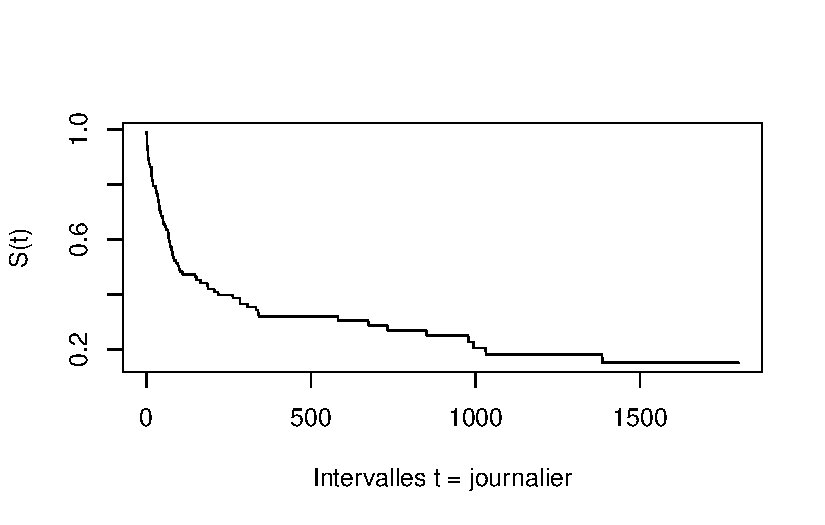
\includegraphics{14-R_files/figure-pdf/unnamed-chunk-4-1.pdf}

}

\end{figure}

\textbf{\emph{Intervalle \(dt=30\)}}

\begin{Shaded}
\begin{Highlighting}[]
\CommentTok{\# On définit un vecteur définissant les intervalles (il n\textquotesingle{}y avait pas plus simple????)}
\NormalTok{dt }\OtherTok{\textless{}{-}} \DecValTok{1}\SpecialCharTok{:}\FunctionTok{ceiling}\NormalTok{(}\FunctionTok{max}\NormalTok{(trans}\SpecialCharTok{$}\NormalTok{stime)}\SpecialCharTok{/}\DecValTok{30}\NormalTok{)}\SpecialCharTok{*}\DecValTok{30}

\CommentTok{\# Base dis avec une nouvelle variable de durée =\textgreater{} timeDisc }

\NormalTok{dis }\OtherTok{\textless{}{-}} \FunctionTok{contToDisc}\NormalTok{(}\AttributeTok{dataShort=}\NormalTok{trans, }\AttributeTok{timeColumn=}\StringTok{"stime"}\NormalTok{, }\AttributeTok{intervalLimits =}\NormalTok{ dt )}

\NormalTok{lt }\OtherTok{\textless{}{-}} \FunctionTok{lifeTable}\NormalTok{(}\AttributeTok{dataShort=}\NormalTok{dis, }\AttributeTok{timeColumn=}\StringTok{"timeDisc"}\NormalTok{, }\AttributeTok{eventColumn =} \StringTok{"died"}\NormalTok{)}

\FunctionTok{plot}\NormalTok{(lt, }\AttributeTok{x =} \DecValTok{1}\SpecialCharTok{:}\FunctionTok{dim}\NormalTok{(lt}\SpecialCharTok{$}\NormalTok{Output)[}\DecValTok{1}\NormalTok{], }\AttributeTok{y =}\NormalTok{ lt}\SpecialCharTok{$}\NormalTok{Output}\SpecialCharTok{$}\NormalTok{S, }\AttributeTok{xlab =} \StringTok{"Intervalles dt = 30 jours"}\NormalTok{, }\AttributeTok{ylab=}\StringTok{"S(t)"}\NormalTok{)}
\end{Highlighting}
\end{Shaded}

\begin{figure}[H]

\caption{Méthode actuarielle avec \texttt{discSurv} (2)}

{\centering 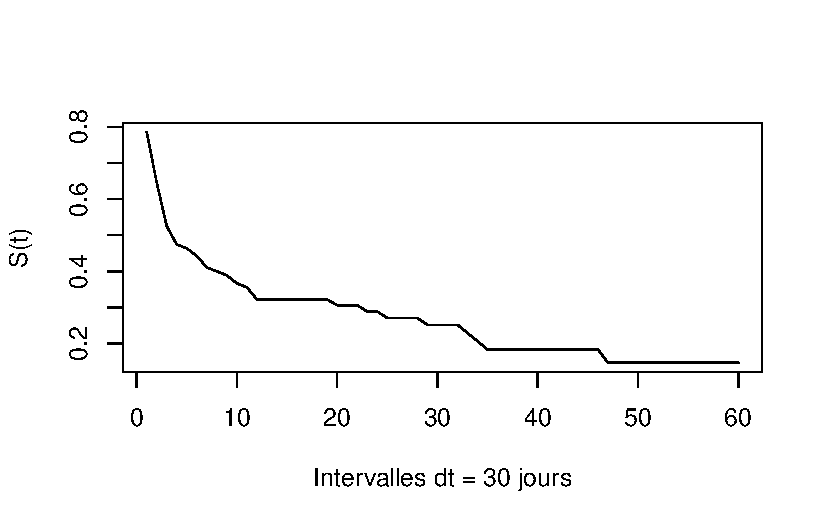
\includegraphics{14-R_files/figure-pdf/unnamed-chunk-5-1.pdf}

}

\end{figure}

Sur les abscisses, ce sont les valeurs des intervalles qui sont
reportés: 10=300 jours. Ce n'est vraiment pas terrible. Pour ce type
d'estimateurs, il est préférable d'utiliser Sas ou Stata.

\hypertarget{muxe9thode-kaplan-meier}{%
\subsection{Méthode Kaplan-Meier}\label{muxe9thode-kaplan-meier}}

Le package survival est le principal outil d'analyse des durée. Le
package \textbf{\texttt{survminer}} permet d'améliorer la présentation
des graphiques.

\textbf{Estimation des fonctions de survie}

Fonction \textbf{\texttt{survfit}}

\begin{codelisting}

\caption{\texttt{syntaxe}}

\begin{Shaded}
\begin{Highlighting}[]
\NormalTok{fit }\OtherTok{\textless{}{-}} \FunctionTok{survfit}\NormalTok{(}\FunctionTok{Surv}\NormalTok{(time, status) }\SpecialCharTok{\textasciitilde{}}\NormalTok{ x, }\AttributeTok{data =}\NormalTok{ base)}
\end{Highlighting}
\end{Shaded}

\end{codelisting}

On peut renseigner directement les variables permettant de calculer la
durée et non la variable de durée elle-même. Cette méthode est utilisée
lorsqu'on introduit une variable dynamique dans un modèle
semi-paramétrique de Cox (\texttt{coxph}).

\begin{codelisting}

\caption{\texttt{Syntaxe}}

\begin{Shaded}
\begin{Highlighting}[]
\NormalTok{fit }\OtherTok{\textless{}{-}} \FunctionTok{survfit}\NormalTok{(}\FunctionTok{Surv}\NormalTok{(variable\_start, variable\_end, status) }\SpecialCharTok{\textasciitilde{}}\NormalTok{ x, }\AttributeTok{data =}\NormalTok{ nom\_base)}
\end{Highlighting}
\end{Shaded}

\end{codelisting}

Sans comparaison de groupes:

\begin{Shaded}
\begin{Highlighting}[]
\NormalTok{fit }\OtherTok{\textless{}{-}} \FunctionTok{survfit}\NormalTok{(}\FunctionTok{Surv}\NormalTok{(stime, died) }\SpecialCharTok{\textasciitilde{}} \DecValTok{1}\NormalTok{, }\AttributeTok{data =}\NormalTok{ trans)}

\NormalTok{fit}
\end{Highlighting}
\end{Shaded}

\begin{verbatim}
Call: survfit(formula = Surv(stime, died) ~ 1, data = trans)

       n events median 0.95LCL 0.95UCL
[1,] 103     75    100      72     263
\end{verbatim}

\begin{Shaded}
\begin{Highlighting}[]
\FunctionTok{summary}\NormalTok{(fit)}
\end{Highlighting}
\end{Shaded}

\begin{verbatim}
Call: survfit(formula = Surv(stime, died) ~ 1, data = trans)

 time n.risk n.event survival std.err lower 95% CI upper 95% CI
    1    103       1    0.990 0.00966       0.9715        1.000
    2    102       3    0.961 0.01904       0.9246        0.999
    3     99       3    0.932 0.02480       0.8847        0.982
    5     96       2    0.913 0.02782       0.8597        0.969
    6     94       2    0.893 0.03043       0.8355        0.955
    8     92       1    0.883 0.03161       0.8237        0.948
    9     91       1    0.874 0.03272       0.8119        0.940
   12     89       1    0.864 0.03379       0.8002        0.933
   16     88       3    0.835 0.03667       0.7656        0.910
   17     85       1    0.825 0.03753       0.7543        0.902
   18     84       1    0.815 0.03835       0.7431        0.894
   21     83       2    0.795 0.03986       0.7208        0.877
   28     81       1    0.785 0.04056       0.7098        0.869
   30     80       1    0.776 0.04122       0.6989        0.861
   32     78       1    0.766 0.04188       0.6878        0.852
   35     77       1    0.756 0.04250       0.6769        0.844
   36     76       1    0.746 0.04308       0.6659        0.835
   37     75       1    0.736 0.04364       0.6551        0.827
   39     74       1    0.726 0.04417       0.6443        0.818
   40     72       2    0.706 0.04519       0.6225        0.800
   43     70       1    0.696 0.04565       0.6117        0.791
   45     69       1    0.686 0.04609       0.6009        0.782
   50     68       1    0.675 0.04650       0.5902        0.773
   51     67       1    0.665 0.04689       0.5796        0.764
   53     66       1    0.655 0.04725       0.5690        0.755
   58     65       1    0.645 0.04759       0.5584        0.746
   61     64       1    0.635 0.04790       0.5479        0.736
   66     63       1    0.625 0.04819       0.5374        0.727
   68     62       2    0.605 0.04870       0.5166        0.708
   69     60       1    0.595 0.04892       0.5063        0.699
   72     59       2    0.575 0.04929       0.4857        0.680
   77     57       1    0.565 0.04945       0.4755        0.670
   78     56       1    0.554 0.04958       0.4654        0.661
   80     55       1    0.544 0.04970       0.4552        0.651
   81     54       1    0.534 0.04979       0.4451        0.641
   85     53       1    0.524 0.04986       0.4351        0.632
   90     52       1    0.514 0.04991       0.4251        0.622
   96     51       1    0.504 0.04994       0.4151        0.612
  100     50       1    0.494 0.04995       0.4052        0.602
  102     49       1    0.484 0.04993       0.3953        0.592
  110     47       1    0.474 0.04992       0.3852        0.582
  149     45       1    0.463 0.04991       0.3749        0.572
  153     44       1    0.453 0.04987       0.3647        0.562
  165     43       1    0.442 0.04981       0.3545        0.551
  186     41       1    0.431 0.04975       0.3440        0.541
  188     40       1    0.420 0.04966       0.3336        0.530
  207     39       1    0.410 0.04954       0.3233        0.519
  219     38       1    0.399 0.04940       0.3130        0.509
  263     37       1    0.388 0.04923       0.3027        0.498
  285     35       2    0.366 0.04885       0.2817        0.475
  308     33       1    0.355 0.04861       0.2713        0.464
  334     32       1    0.344 0.04834       0.2610        0.453
  340     31       1    0.333 0.04804       0.2507        0.442
  342     29       1    0.321 0.04773       0.2401        0.430
  583     21       1    0.306 0.04785       0.2252        0.416
  675     17       1    0.288 0.04830       0.2073        0.400
  733     16       1    0.270 0.04852       0.1898        0.384
  852     14       1    0.251 0.04873       0.1712        0.367
  979     11       1    0.228 0.04934       0.1491        0.348
  995     10       1    0.205 0.04939       0.1279        0.329
 1032      9       1    0.182 0.04888       0.1078        0.308
 1386      6       1    0.152 0.04928       0.0804        0.287
\end{verbatim}

\begin{Shaded}
\begin{Highlighting}[]
\FunctionTok{plot}\NormalTok{(fit)}
\end{Highlighting}
\end{Shaded}

\begin{figure}[H]

{\centering 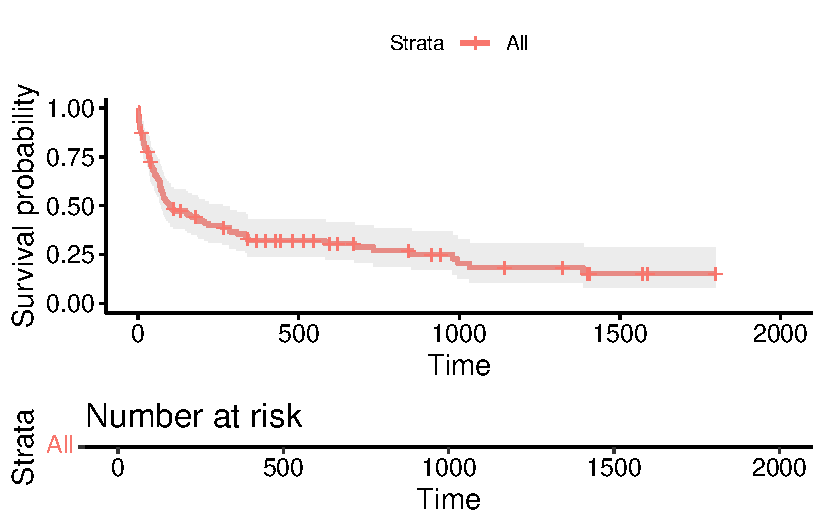
\includegraphics{14-R_files/figure-pdf/unnamed-chunk-8-1.pdf}

}

\end{figure}

Le premier output \texttt{fit} permet d'obtenir la durée médiane, ici
égale à 100 (\(S(100)=0.494\)). Le second avec la fonction
\textbf{\texttt{summary}} permet d'obtenir une table des estimateurs. La
fonction de survie peut être tracée avec la fonction
\textbf{\texttt{plot}} (en pointillés les intervalles de confiance).

On peut obtenir des graphes de meilleur qualité avec la librairie
\textbf{\texttt{survminer}}, avec la fonction
\textbf{\texttt{ggsurvplot}}

\begin{Shaded}
\begin{Highlighting}[]
\FunctionTok{ggsurvplot}\NormalTok{(fit, }\AttributeTok{conf.int =} \ConstantTok{TRUE}\NormalTok{)}
\end{Highlighting}
\end{Shaded}

\begin{figure}[H]

{\centering 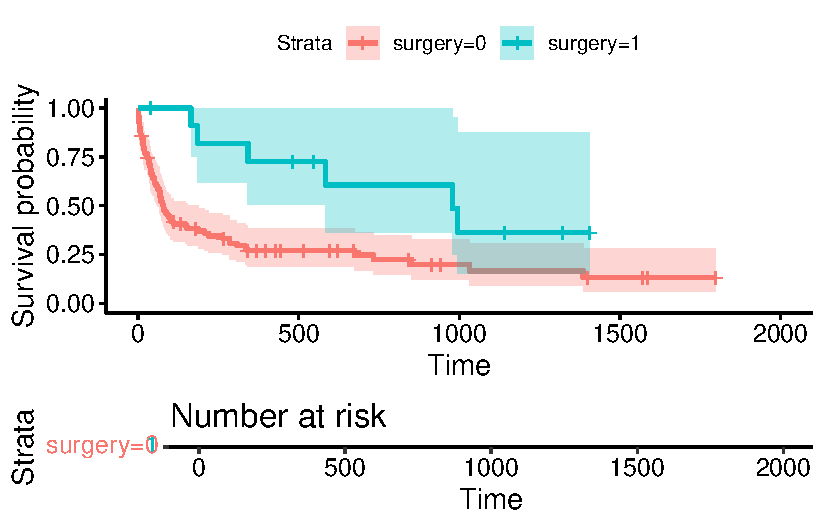
\includegraphics{14-R_files/figure-pdf/unnamed-chunk-9-1.pdf}

}

\end{figure}

On peut ajouter la population encore soumise au risque à plusieurs
points d'observation avec l'argument \texttt{risk.table\ =\ TRUE}

\begin{Shaded}
\begin{Highlighting}[]
\FunctionTok{ggsurvplot}\NormalTok{(fit, }\AttributeTok{conf.int =} \ConstantTok{TRUE}\NormalTok{, }\AttributeTok{risk.table =} \ConstantTok{TRUE}\NormalTok{)}
\end{Highlighting}
\end{Shaded}

\begin{figure}[H]

{\centering 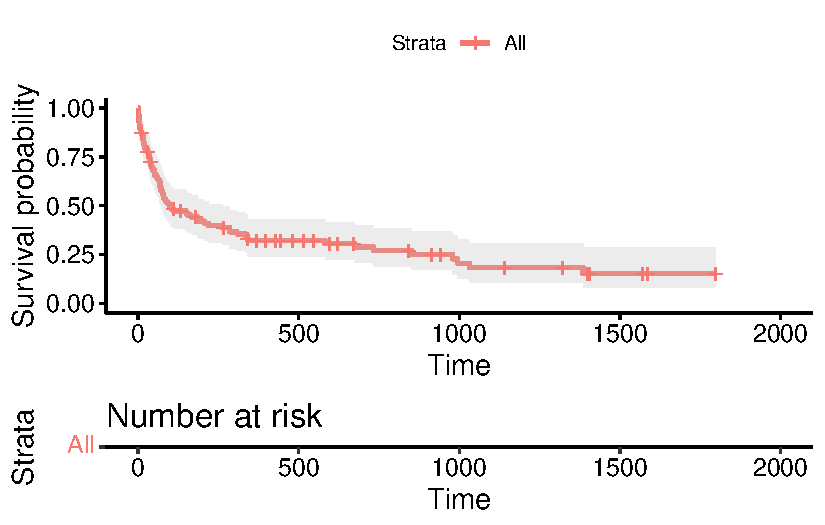
\includegraphics{14-R_files/figure-pdf/unnamed-chunk-10-1.pdf}

}

\end{figure}

\hypertarget{comparaison-des-st-muxe9thode-km}{%
\subsection{Comparaison des S(t) méthode
KM}\label{comparaison-des-st-muxe9thode-km}}

On va comparer les deuxfonctions de survie pour la variable
\emph{surgery}, celle pour les personnes non opérées et celle pour les
personnes opérées.

\begin{Shaded}
\begin{Highlighting}[]
\NormalTok{fit }\OtherTok{\textless{}{-}} \FunctionTok{survfit}\NormalTok{(}\FunctionTok{Surv}\NormalTok{(stime, died) }\SpecialCharTok{\textasciitilde{}}\NormalTok{ surgery, }\AttributeTok{data =}\NormalTok{ trans)}
\NormalTok{fit}
\end{Highlighting}
\end{Shaded}

\begin{verbatim}
Call: survfit(formula = Surv(stime, died) ~ surgery, data = trans)

           n events median 0.95LCL 0.95UCL
surgery=0 91     69     78      61     153
surgery=1 12      6    979     583      NA
\end{verbatim}

\begin{Shaded}
\begin{Highlighting}[]
\FunctionTok{ggsurvplot}\NormalTok{(fit, }\AttributeTok{conf.int =} \ConstantTok{TRUE}\NormalTok{, }\AttributeTok{risk.table =} \ConstantTok{TRUE}\NormalTok{)}
\end{Highlighting}
\end{Shaded}

\begin{figure}[H]

{\centering 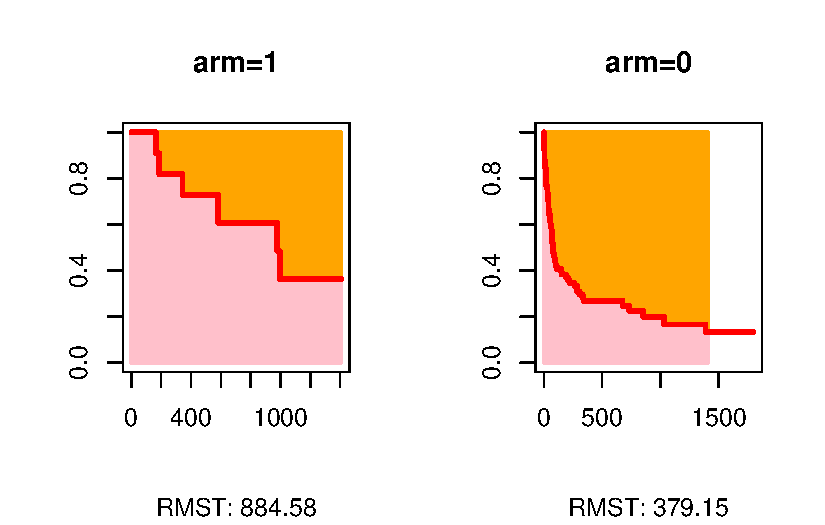
\includegraphics{14-R_files/figure-pdf/unnamed-chunk-11-1.pdf}

}

\end{figure}

\textbf{Tests du logrank}

On utilise la fonction \textbf{\texttt{survdiff}}, avec comme variante
le test de Peto-Peto (\texttt{rho=1}).\\
La syntaxe est quasiment identique à la fonction \texttt{survdiff}.

\begin{Shaded}
\begin{Highlighting}[]
\FunctionTok{survdiff}\NormalTok{(}\FunctionTok{Surv}\NormalTok{(stime, died) }\SpecialCharTok{\textasciitilde{}}\NormalTok{ surgery, }\AttributeTok{rho=}\DecValTok{1}\NormalTok{, }\AttributeTok{data =}\NormalTok{ trans)}
\end{Highlighting}
\end{Shaded}

\begin{verbatim}
Call:
survdiff(formula = Surv(stime, died) ~ surgery, data = trans, 
    rho = 1)

           N Observed Expected (O-E)^2/E (O-E)^2/V
surgery=0 91    45.28    39.12     0.968      8.65
surgery=1 12     2.03     8.18     4.630      8.65

 Chisq= 8.7  on 1 degrees of freedom, p= 0.003 
\end{verbatim}

Ici la variable est binaire. Si on veux tester deux à deux les niveaux
d'une variable catégorielle à plus de deux modalités, il est fortement
conseillé d'utiliser la fonction \textbf{\texttt{pairwise\_survdiff}} de
\texttt{survminer} (syntaxe identique que \texttt{survdiff}).

\textbf{Comparaison des RMST}

La fonction \textbf{\texttt{rmst2}} du package \textbf{\texttt{survRM2}}
permet de comparer les RMST entre 2 groupes . La strate pour les
comparaisons doit être impérativement renommée \emph{arm}. La fonction,
issue d'une commande de Stata, n'est pas très souple.

\begin{Shaded}
\begin{Highlighting}[]
\NormalTok{trans}\SpecialCharTok{$}\NormalTok{arm}\OtherTok{=}\NormalTok{trans}\SpecialCharTok{$}\NormalTok{surgery}
\NormalTok{a}\OtherTok{=}\FunctionTok{rmst2}\NormalTok{(trans}\SpecialCharTok{$}\NormalTok{stime, trans}\SpecialCharTok{$}\NormalTok{died, trans}\SpecialCharTok{$}\NormalTok{arm, }\AttributeTok{tau=}\ConstantTok{NULL}\NormalTok{)}
\FunctionTok{print}\NormalTok{(a)}
\end{Highlighting}
\end{Shaded}

\begin{verbatim}

The truncation time, tau, was not specified. Thus, the default tau  1407  is used. 

Restricted Mean Survival Time (RMST) by arm 
                Est.      se lower .95 upper .95
RMST (arm=1) 884.576 151.979   586.702  1182.450
RMST (arm=0) 379.148  58.606   264.283   494.012


Restricted Mean Time Lost (RMTL) by arm 
                 Est.      se lower .95 upper .95
RMTL (arm=1)  522.424 151.979   224.550   820.298
RMTL (arm=0) 1027.852  58.606   912.988  1142.717


Between-group contrast 
                        Est. lower .95 upper .95     p
RMST (arm=1)-(arm=0) 505.428   186.175   824.682 0.002
RMST (arm=1)/(arm=0)   2.333     1.483     3.670 0.000
RMTL (arm=1)/(arm=0)   0.508     0.284     0.909 0.022
\end{verbatim}

\begin{Shaded}
\begin{Highlighting}[]
\FunctionTok{plot}\NormalTok{(a)}
\end{Highlighting}
\end{Shaded}

\begin{figure}[H]

{\centering 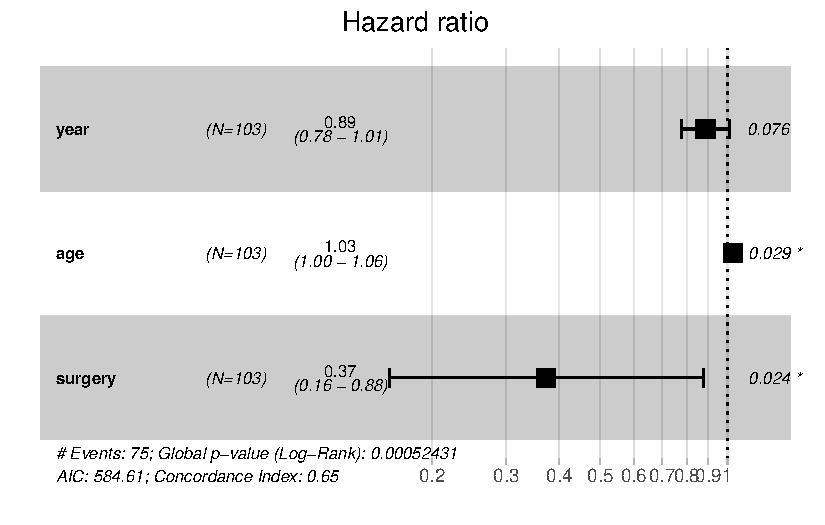
\includegraphics{14-R_files/figure-pdf/unnamed-chunk-13-1.pdf}

}

\end{figure}

\hypertarget{moduxe8le-de-cox-1}{%
\section{Modèle de Cox}\label{moduxe8le-de-cox-1}}

Ici tout est estimé de nouveau avec des fonctions du package
\texttt{survival}:

\begin{itemize}
\tightlist
\item
  Estimation du modèle: \texttt{coxph}.
\item
  Test de Grambsch-Therneau: \texttt{cox.zph} et \texttt{cox.oldzph}.
\item
  Introduction d'une variable dynamique: allongement de la base avec
  \texttt{survsplit}.
\end{itemize}

\hypertarget{estimation-du-moduxe8le}{%
\subsection{Estimation du modèle}\label{estimation-du-moduxe8le}}

Par défaut, R utilise la correction d'Efron pour les évènements
simultanés. Il est préférable de ne pas la modifier.

Syntaxe:

\begin{codelisting}

\caption{\texttt{Syntaxe}}

\begin{Shaded}
\begin{Highlighting}[]
\NormalTok{coxph(Surv(time, status) \textasciitilde{} x1 + x2 + ....., data=base, ties=}\StringTok{"nom\_correction"}\NormalTok{))}
\end{Highlighting}
\end{Shaded}

\end{codelisting}

\begin{Shaded}
\begin{Highlighting}[]
\NormalTok{coxfit }\OtherTok{=} \FunctionTok{coxph}\NormalTok{(}\AttributeTok{formula =} \FunctionTok{Surv}\NormalTok{(stime, died) }\SpecialCharTok{\textasciitilde{}}\NormalTok{ year }\SpecialCharTok{+}\NormalTok{ age }\SpecialCharTok{+}\NormalTok{ surgery, }\AttributeTok{data =}\NormalTok{ trans)}
\FunctionTok{summary}\NormalTok{(coxfit)}
\end{Highlighting}
\end{Shaded}

\begin{verbatim}
Call:
coxph(formula = Surv(stime, died) ~ year + age + surgery, data = trans)

  n= 103, number of events= 75 

            coef exp(coef) se(coef)      z Pr(>|z|)
year    -0.11963   0.88725  0.06734 -1.776   0.0757
age      0.02958   1.03002  0.01352  2.187   0.0287
surgery -0.98732   0.37257  0.43626 -2.263   0.0236

        exp(coef) exp(-coef) lower .95 upper .95
year       0.8872     1.1271    0.7775    1.0124
age        1.0300     0.9709    1.0031    1.0577
surgery    0.3726     2.6840    0.1584    0.8761

Concordance= 0.653  (se = 0.032 )
Likelihood ratio test= 17.63  on 3 df,   p=5e-04
Wald test            = 15.76  on 3 df,   p=0.001
Score (logrank) test = 16.71  on 3 df,   p=8e-04
\end{verbatim}

\begin{Shaded}
\begin{Highlighting}[]
\FunctionTok{tbl\_regression}\NormalTok{(coxfit, }\AttributeTok{exponentiate =} \ConstantTok{TRUE}\NormalTok{,)}
\end{Highlighting}
\end{Shaded}

\begin{verbatim}
Table printed with `knitr::kable()`, not {gt}. Learn why at
https://www.danieldsjoberg.com/gtsummary/articles/rmarkdown.html
To suppress this message, include `message = FALSE` in code chunk header.
\end{verbatim}

\begin{longtable}[]{@{}lccc@{}}
\toprule\noalign{}
\textbf{Characteristic} & \textbf{HR} & \textbf{95\% CI} &
\textbf{p-value} \\
\midrule\noalign{}
\endhead
\bottomrule\noalign{}
\endlastfoot
year & 0.89 & 0.78, 1.01 & 0.076 \\
age & 1.03 & 1.00, 1.06 & 0.029 \\
surgery & 0.37 & 0.16, 0.88 & 0.024 \\
\end{longtable}

L'output des résultats reporte le logarithme des Risques Ratios (coef)
ainsi que les RR (exp(coef)). Il est intéressant de regarder la valeur
de concordance (Harrel's) qui donne des indications sur la qualité de
l'ajustement (proche de l'AUC/ROC d'un modèle probabiliste standard).

On peut représenter sous forme graphique les résultats avec la fonction
\textbf{\texttt{ggforest}} de \texttt{survminer}

\begin{Shaded}
\begin{Highlighting}[]
\FunctionTok{ggforest}\NormalTok{(coxfit)}
\end{Highlighting}
\end{Shaded}

\begin{verbatim}
Warning in .get_data(model, data = data): The `data` argument is not provided.
Data will be extracted from model fit.
\end{verbatim}

\begin{figure}[H]

{\centering 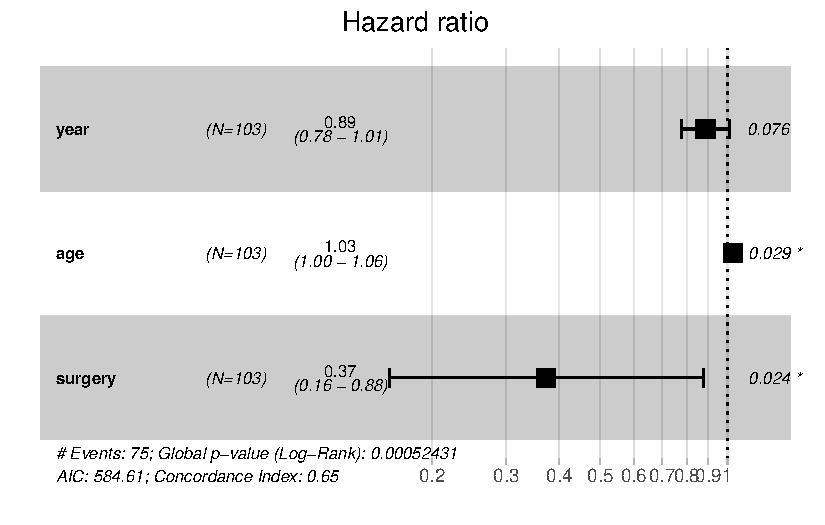
\includegraphics{14-R_files/figure-pdf/unnamed-chunk-16-1.pdf}

}

\end{figure}

\hypertarget{hypothuxe8se-ph}{%
\subsection{Hypothèse PH}\label{hypothuxe8se-ph}}

\hypertarget{test-grambsch-therneau}{%
\subsubsection{Test Grambsch-Therneau}\label{test-grambsch-therneau}}

\textbf{Résidus de Schoenfeld}

On utilise la fonction \textbf{\texttt{cox.zph}} pour effectuer le test
GLS (moindre carrés généralisés) qui a été substitué au test OLS
(moindres carrés ordinaires) avec le passage à la v3 du package.
\textbf{Je donne plus loin un moyen de récupérer et d'exécuter le test
OLS, que je conseille d'utiliser en présence de durées
discrètes/groupées}.

Le test peut utiliser plusieurs fonctions de la durée. Par défaut la
fonction utilise \(1-KM\), soit le complémentaire de l'estimateur de
Kaplan-Meier (option \texttt{transform="km"}).

\begin{itemize}
\tightlist
\item
  \textbf{Test GLS (V3 de survival)}
\end{itemize}

Avec \texttt{transform="km"}

\begin{Shaded}
\begin{Highlighting}[]
\FunctionTok{cox.zph}\NormalTok{(coxfit)}
\end{Highlighting}
\end{Shaded}

\begin{verbatim}
        chisq df     p
year    3.309  1 0.069
age     0.922  1 0.337
surgery 5.494  1 0.019
GLOBAL  8.581  3 0.035
\end{verbatim}

Avec \texttt{transform="identity"} (\(f(t)=t\))

\begin{Shaded}
\begin{Highlighting}[]
\FunctionTok{cox.zph}\NormalTok{(coxfit, }\AttributeTok{transform=}\StringTok{"identity"}\NormalTok{)}
\end{Highlighting}
\end{Shaded}

\begin{verbatim}
        chisq df     p
year     4.54  1 0.033
age      1.71  1 0.191
surgery  4.92  1 0.027
GLOBAL   9.47  3 0.024
\end{verbatim}

Remarque: avec la v3 de survival, quelques options ont été ajoutées tel
que \emph{\texttt{terms}} qui permet pour une variable catégorielle à
plus de deux modalités de choisir entre un sous test multiple sur la
variable (k modalités =\textgreater{} k-1 degré de liberté) et une série
de tests à 1 degré de liberté sur chaque modalité (k-1 tests). De mon
point de vue préférer la seconde solution avec
\textbf{\texttt{terms=FALSE}}. le test de Grambsch-Therneau est
particulièrement sensible au nombre de degré de liberté, et il convient
donc d'éviter de l'utiliser dans un cadre multiple.

\begin{itemize}
\tightlist
\item
  \textbf{Test OLS (V2 de survival - Stata - Sas - Python)}
\end{itemize}

\begin{codelisting}

\caption{\texttt{Récupération du test ols}}

\begin{Shaded}
\begin{Highlighting}[]
\FunctionTok{source}\NormalTok{(}\StringTok{"https://raw.githubusercontent.com/mthevenin/analyse\_duree/main/cox.zphold/cox.zphold.R"}\NormalTok{)}
\end{Highlighting}
\end{Shaded}

\end{codelisting}

\begin{codelisting}

\caption{\texttt{Exécution du test ols}}

\begin{Shaded}
\begin{Highlighting}[]
\FunctionTok{cox.zphold}\NormalTok{(coxfit, }\AttributeTok{transform=}\StringTok{"identity"}\NormalTok{)}
\end{Highlighting}
\end{Shaded}

\end{codelisting}

\begin{verbatim}
          rho chisq      p
year    0.102 0.797 0.3720
age     0.129 1.612 0.2043
surgery 0.297 5.539 0.0186
GLOBAL     NA 8.756 0.0327
\end{verbatim}

\hypertarget{introduction-dune-intuxe9raction}{%
\subsubsection{Introduction d'une
intéraction}\label{introduction-dune-intuxe9raction}}

Lorsque la covariable n'est pas continue, elle doit être impérativement
transformée en indicatrice \footnote{c'est le cas ici, la variable
  \emph{surgery} est bien codée (0;1)}. Penser à vérifier en amont que
les résultats du modèle sont bien identiques avec le modèle estimé
précédemment (ne pas oublier d'omettre le niveau en référence).

La variable d'intéraction est \textbf{\texttt{tt(nom\_variable)}}, la
fonction de la durée (ici forme linéaire simple) est indiquée en option
de la fonction: \textbf{\texttt{tt\ =\ function(x,\ t,\ ...)\ x*t}}.

\begin{Shaded}
\begin{Highlighting}[]
\NormalTok{coxfit2 }\OtherTok{=} \FunctionTok{coxph}\NormalTok{(}\AttributeTok{formula =} \FunctionTok{Surv}\NormalTok{(stime, died) }\SpecialCharTok{\textasciitilde{}}\NormalTok{ year }\SpecialCharTok{+}\NormalTok{ age }\SpecialCharTok{+}\NormalTok{ surgery }\SpecialCharTok{+} \FunctionTok{tt}\NormalTok{(surgery), }\AttributeTok{data =}\NormalTok{ trans, }\AttributeTok{tt =} \ControlFlowTok{function}\NormalTok{(x, t, ...) x}\SpecialCharTok{*}\NormalTok{t)}

\FunctionTok{summary}\NormalTok{(coxfit2)}
\end{Highlighting}
\end{Shaded}

\begin{verbatim}
Call:
coxph(formula = Surv(stime, died) ~ year + age + surgery + tt(surgery), 
    data = trans, tt = function(x, t, ...) x * t)

  n= 103, number of events= 75 

                 coef exp(coef)  se(coef)      z Pr(>|z|)
year        -0.123074  0.884198  0.066835 -1.841  0.06555
age          0.028888  1.029310  0.013449  2.148  0.03172
surgery     -1.754738  0.172953  0.674391 -2.602  0.00927
tt(surgery)  0.002231  1.002234  0.001102  2.024  0.04299

            exp(coef) exp(-coef) lower .95 upper .95
year           0.8842     1.1310   0.77564    1.0080
age            1.0293     0.9715   1.00253    1.0568
surgery        0.1730     5.7819   0.04612    0.6486
tt(surgery)    1.0022     0.9978   1.00007    1.0044

Concordance= 0.656  (se = 0.032 )
Likelihood ratio test= 21.58  on 4 df,   p=2e-04
Wald test            = 16.99  on 4 df,   p=0.002
Score (logrank) test = 19  on 4 df,   p=8e-04
\end{verbatim}

\begin{Shaded}
\begin{Highlighting}[]
\FunctionTok{tbl\_regression}\NormalTok{(coxfit2, }\AttributeTok{exponentiate =} \ConstantTok{TRUE}\NormalTok{, }\AttributeTok{estimate\_fun =}\NormalTok{ purrr}\SpecialCharTok{::}\FunctionTok{partial}\NormalTok{(style\_ratio, }\AttributeTok{digits =} \DecValTok{3}\NormalTok{))}
\end{Highlighting}
\end{Shaded}

\begin{verbatim}
Table printed with `knitr::kable()`, not {gt}. Learn why at
https://www.danieldsjoberg.com/gtsummary/articles/rmarkdown.html
To suppress this message, include `message = FALSE` in code chunk header.
\end{verbatim}

\begin{longtable}[]{@{}lccc@{}}
\toprule\noalign{}
\textbf{Characteristic} & \textbf{HR} & \textbf{95\% CI} &
\textbf{p-value} \\
\midrule\noalign{}
\endhead
\bottomrule\noalign{}
\endlastfoot
year & 0.884 & 0.776, 1.008 & 0.066 \\
age & 1.029 & 1.003, 1.057 & 0.032 \\
surgery & 0.173 & 0.046, 0.649 & 0.009 \\
tt(surgery) & 1.002 & 1.000, 1.004 & 0.043 \\
\end{longtable}

\textbf{Rappel}: le paramètre estimé pour \textbf{\texttt{tt(surgery)}}
ne reporte pas un rapport de risques, mais un rapport de de deux
rapports de risques. C'est bien une double différence sur l'échelle
d'estimation (log).

\hypertarget{introduction-dune-variable-dynamique-binaire}{%
\subsection{Introduction d'une variable dynamique
(binaire)}\label{introduction-dune-variable-dynamique-binaire}}

La dimension dynamique est ici le fait d'avoir été opéré pour une greffe
du coeur.

\begin{itemize}
\item
  \textbf{Etape 1}: créer un vecteur donnant les durées aux temps
  d'évènement.
\item
  \textbf{Etape 2}: appliquer ce vecteurs de points de coupure à la
  fonction \texttt{survsplit}.
\item
  \textbf{Etape 3}: modifier la variable transplant (ou créer une
  nouvelle) à l'aide de la variable \textbf{wait} qui prend la valeur 1
  à partir du jour de la greffe, 0 avant.
\item
  \emph{Etape 1}: création de l'objet cut (vecteur), qui récupère les
  moments où au moins un évènement est observé.
\end{itemize}

\begin{Shaded}
\begin{Highlighting}[]
\NormalTok{cut}\OtherTok{=} \FunctionTok{unique}\NormalTok{(trans}\SpecialCharTok{$}\NormalTok{stime[trans}\SpecialCharTok{$}\NormalTok{died }\SpecialCharTok{==} \DecValTok{1}\NormalTok{])}

\NormalTok{cut}
\end{Highlighting}
\end{Shaded}

\begin{verbatim}
 [1]    1    2    3    5    6    8    9   12   16   17   18   21   28   30   32
[16]   35   36   37   39   40   43   45   50   51   53   58   61   66   68   69
[31]   72   77   78   80   81   85   90   96  100  102  110  149  153  165  186
[46]  188  207  219  263  285  308  334  340  342  583  675  733  852  979  995
[61] 1032 1386
\end{verbatim}

\emph{Etape 2}: allonger la base aux durées d'évènement

\begin{Shaded}
\begin{Highlighting}[]
\NormalTok{tvc }\OtherTok{=} \FunctionTok{survSplit}\NormalTok{(}\AttributeTok{data =}\NormalTok{ trans, }\AttributeTok{cut =}\NormalTok{ cut, }\AttributeTok{end =} \StringTok{"stime"}\NormalTok{, }\AttributeTok{start =} \StringTok{"stime0"}\NormalTok{, }\AttributeTok{event =} \StringTok{"died"}\NormalTok{)}

\FunctionTok{head}\NormalTok{(tvc, }\AttributeTok{n=}\DecValTok{20}\NormalTok{ )}
\end{Highlighting}
\end{Shaded}

\begin{verbatim}
   id year age surgery transplant wait mois compet arm stime0 stime died
1  15   68  53       0          0    0    1      1   0      0     1    1
2  43   70  43       0          0    0    1      1   0      0     1    0
3  43   70  43       0          0    0    1      1   0      1     2    1
4  61   71  52       0          0    0    1      1   0      0     1    0
5  61   71  52       0          0    0    1      1   0      1     2    1
6  75   72  52       0          0    0    1      1   0      0     1    0
7  75   72  52       0          0    0    1      1   0      1     2    1
8   6   68  54       0          0    0    1      2   0      0     1    0
9   6   68  54       0          0    0    1      2   0      1     2    0
10  6   68  54       0          0    0    1      2   0      2     3    1
11 42   70  36       0          0    0    1      1   0      0     1    0
12 42   70  36       0          0    0    1      1   0      1     2    0
13 42   70  36       0          0    0    1      1   0      2     3    1
14 54   71  47       0          0    0    1      1   0      0     1    0
15 54   71  47       0          0    0    1      1   0      1     2    0
16 54   71  47       0          0    0    1      1   0      2     3    1
17 38   70  41       0          1    5    1      1   0      0     1    0
18 38   70  41       0          1    5    1      1   0      1     2    0
19 38   70  41       0          1    5    1      1   0      2     3    0
20 38   70  41       0          1    5    1      1   0      3     5    1
\end{verbatim}

On vérifie qu'on obtient les même résultats avec le modèle sans tvc

\begin{Shaded}
\begin{Highlighting}[]
\FunctionTok{coxph}\NormalTok{(}\AttributeTok{formula =} \FunctionTok{Surv}\NormalTok{(stime0, stime, died) }\SpecialCharTok{\textasciitilde{}}\NormalTok{ year }\SpecialCharTok{+}\NormalTok{ age }\SpecialCharTok{+}\NormalTok{ surgery, }\AttributeTok{data =}\NormalTok{ tvc)}
\end{Highlighting}
\end{Shaded}

\begin{verbatim}
Call:
coxph(formula = Surv(stime0, stime, died) ~ year + age + surgery, 
    data = tvc)

            coef exp(coef) se(coef)      z      p
year    -0.11963   0.88725  0.06734 -1.776 0.0757
age      0.02958   1.03002  0.01352  2.187 0.0287
surgery -0.98732   0.37257  0.43626 -2.263 0.0236

Likelihood ratio test=17.63  on 3 df, p=0.0005243
n= 3573, number of events= 75 
\end{verbatim}

\begin{itemize}
\tightlist
\item
  \emph{Etape 3}: on génère la variable dynamique de sorte que les
  personnes n'apparaissent pas greffés avant l'opération
\end{itemize}

\begin{Shaded}
\begin{Highlighting}[]
\NormalTok{tvc}\SpecialCharTok{$}\NormalTok{tvc}\OtherTok{=}\FunctionTok{ifelse}\NormalTok{(tvc}\SpecialCharTok{$}\NormalTok{transplant}\SpecialCharTok{==}\DecValTok{1} \SpecialCharTok{\&}\NormalTok{ tvc}\SpecialCharTok{$}\NormalTok{wait}\SpecialCharTok{\textless{}=}\NormalTok{tvc}\SpecialCharTok{$}\NormalTok{stime,}\DecValTok{1}\NormalTok{,}\DecValTok{0}\NormalTok{)}
\end{Highlighting}
\end{Shaded}

\textbf{Estimation du modèle}\\
En format long, on doit préciser dans la formule l'intervalle de durée
avec les variables stime0 (début) et stime(fin)

\begin{Shaded}
\begin{Highlighting}[]
\NormalTok{tvcfit }\OtherTok{=} \FunctionTok{coxph}\NormalTok{(}\AttributeTok{formula =} \FunctionTok{Surv}\NormalTok{(stime0, stime, died) }\SpecialCharTok{\textasciitilde{}}\NormalTok{ year }\SpecialCharTok{+}\NormalTok{ age }\SpecialCharTok{+}\NormalTok{ surgery }\SpecialCharTok{+}\NormalTok{ tvc, }\AttributeTok{data =}\NormalTok{ tvc)}

\FunctionTok{summary}\NormalTok{(tvcfit)}
\end{Highlighting}
\end{Shaded}

\begin{verbatim}
Call:
coxph(formula = Surv(stime0, stime, died) ~ year + age + surgery + 
    tvc, data = tvc)

  n= 3573, number of events= 75 

            coef exp(coef) se(coef)      z Pr(>|z|)
year    -0.12032   0.88664  0.06734 -1.787   0.0740
age      0.03044   1.03091  0.01390  2.190   0.0285
surgery -0.98289   0.37423  0.43655 -2.251   0.0244
tvc     -0.08221   0.92108  0.30484 -0.270   0.7874

        exp(coef) exp(-coef) lower .95 upper .95
year       0.8866      1.128    0.7770    1.0117
age        1.0309      0.970    1.0032    1.0594
surgery    0.3742      2.672    0.1591    0.8805
tvc        0.9211      1.086    0.5068    1.6741

Concordance= 0.659  (se = 0.032 )
Likelihood ratio test= 17.7  on 4 df,   p=0.001
Wald test            = 15.79  on 4 df,   p=0.003
Score (logrank) test = 16.74  on 4 df,   p=0.002
\end{verbatim}

\begin{Shaded}
\begin{Highlighting}[]
\FunctionTok{tbl\_regression}\NormalTok{(tvcfit, }\AttributeTok{exponentiate =} \ConstantTok{TRUE}\NormalTok{, }\AttributeTok{estimate\_fun =}\NormalTok{ purrr}\SpecialCharTok{::}\FunctionTok{partial}\NormalTok{(style\_ratio, }\AttributeTok{digits =} \DecValTok{3}\NormalTok{))}
\end{Highlighting}
\end{Shaded}

\begin{verbatim}
Table printed with `knitr::kable()`, not {gt}. Learn why at
https://www.danieldsjoberg.com/gtsummary/articles/rmarkdown.html
To suppress this message, include `message = FALSE` in code chunk header.
\end{verbatim}

\begin{longtable}[]{@{}lccc@{}}
\toprule\noalign{}
\textbf{Characteristic} & \textbf{HR} & \textbf{95\% CI} &
\textbf{p-value} \\
\midrule\noalign{}
\endhead
\bottomrule\noalign{}
\endlastfoot
year & 0.887 & 0.777, 1.012 & 0.074 \\
age & 1.031 & 1.003, 1.059 & 0.029 \\
surgery & 0.374 & 0.159, 0.880 & 0.024 \\
tvc & 0.921 & 0.507, 1.674 & 0.8 \\
\end{longtable}

\begin{Shaded}
\begin{Highlighting}[]
\FunctionTok{ggforest}\NormalTok{(tvcfit)}
\end{Highlighting}
\end{Shaded}

\begin{verbatim}
Warning in .get_data(model, data = data): The `data` argument is not provided.
Data will be extracted from model fit.
\end{verbatim}

\begin{figure}[H]

{\centering 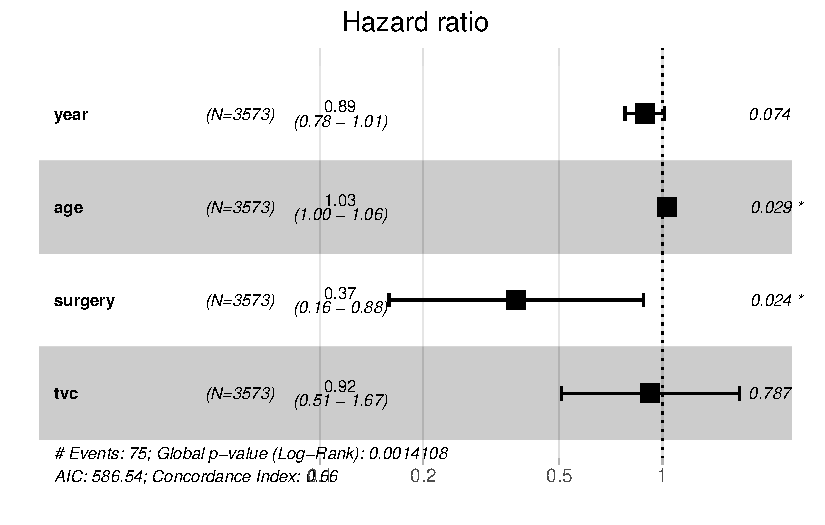
\includegraphics{14-R_files/figure-pdf/unnamed-chunk-27-1.pdf}

}

\end{figure}

\hypertarget{analyse-en-duruxe9e-discruxe8te}{%
\section{\texorpdfstring{\textbf{Analyse en durée
discrète}}{Analyse en durée discrète}}\label{analyse-en-duruxe9e-discruxe8te}}

Pour la durée, on va utiliser la variable mois (regroupement sur 30
jours).

La fonction \textbf{\texttt{uncount}} du package \texttt{tidyr}
permettra de splitter la base aux durées d'observation. C'est ici la
principale différence avec le modèle de Cox qui est une estimation aux
durées d'évènement

\begin{Shaded}
\begin{Highlighting}[]
\NormalTok{trans }\OtherTok{\textless{}{-}} \FunctionTok{read.csv}\NormalTok{(}\StringTok{"https://raw.githubusercontent.com/mthevenin/analyse\_duree/master/bases/transplantation.csv"}\NormalTok{)}
\end{Highlighting}
\end{Shaded}

La variable \emph{mois}, va être supprimée avec \texttt{uncount}. Comme
on en aura besoin plus loin pour générer proprement la variable
évènement, on peut créer ici une variable mirroir.

\begin{Shaded}
\begin{Highlighting}[]
\NormalTok{trans}\SpecialCharTok{$}\NormalTok{T }\OtherTok{=}\NormalTok{ trans}\SpecialCharTok{$}\NormalTok{mois}
\end{Highlighting}
\end{Shaded}

\begin{Shaded}
\begin{Highlighting}[]
\NormalTok{dt }\OtherTok{=} \FunctionTok{uncount}\NormalTok{(trans,mois)}
\NormalTok{dt }\OtherTok{=}\NormalTok{ dt[}\FunctionTok{order}\NormalTok{(dt}\SpecialCharTok{$}\NormalTok{id),]}
\end{Highlighting}
\end{Shaded}

\begin{Shaded}
\begin{Highlighting}[]
\FunctionTok{head}\NormalTok{(dt,}\DecValTok{11}\NormalTok{) }
\end{Highlighting}
\end{Shaded}

\begin{verbatim}
    id year age died stime surgery transplant wait compet  T
48   1   67  30    1    50       0          0    0      1  2
49   1   67  30    1    50       0          0    0      1  2
10   2   68  51    1     6       0          0    0      1  1
18   3   68  54    1    16       0          1    1      1  1
36   4   68  40    1    39       0          1   36      2  2
37   4   68  40    1    39       0          1   36      2  2
20   5   68  20    1    18       0          0    0      1  1
5    6   68  54    1     3       0          0    0      2  1
466  7   68  50    1   675       0          1   51      1 23
467  7   68  50    1   675       0          1   51      1 23
468  7   68  50    1   675       0          1   51      1 23
\end{verbatim}

On va générer une variable type compteur pour mesurer la durée à chaque
point d'observation.

\begin{Shaded}
\begin{Highlighting}[]
\NormalTok{dt}\SpecialCharTok{$}\NormalTok{x}\OtherTok{=}\DecValTok{1}
\NormalTok{dt}\SpecialCharTok{$}\NormalTok{t }\OtherTok{=} \FunctionTok{ave}\NormalTok{(dt}\SpecialCharTok{$}\NormalTok{x,dt}\SpecialCharTok{$}\NormalTok{id, }\AttributeTok{FUN=}\NormalTok{cumsum)}

\FunctionTok{head}\NormalTok{(dt, }\AttributeTok{n=}\DecValTok{8}\NormalTok{)}
\end{Highlighting}
\end{Shaded}

\begin{verbatim}
   id year age died stime surgery transplant wait compet T x t
48  1   67  30    1    50       0          0    0      1 2 1 1
49  1   67  30    1    50       0          0    0      1 2 1 2
10  2   68  51    1     6       0          0    0      1 1 1 1
18  3   68  54    1    16       0          1    1      1 1 1 1
36  4   68  40    1    39       0          1   36      2 2 1 1
37  4   68  40    1    39       0          1   36      2 2 1 2
20  5   68  20    1    18       0          0    0      1 1 1 1
5   6   68  54    1     3       0          0    0      2 1 1 1
\end{verbatim}

Si un individu est décédé, died=1 est reporté sur toute les lignes (idem
qu'avec la variable dynamique). On va modifier la variable tel que
\emph{died=0 si t\textless T\$}.

\begin{Shaded}
\begin{Highlighting}[]
\NormalTok{dt }\OtherTok{=} \FunctionTok{arrange}\NormalTok{(dt,id,t)}

\NormalTok{dt}\SpecialCharTok{$}\NormalTok{died[dt}\SpecialCharTok{$}\NormalTok{t}\SpecialCharTok{\textless{}}\NormalTok{dt}\SpecialCharTok{$}\NormalTok{T]}\OtherTok{=}\DecValTok{0}

\FunctionTok{head}\NormalTok{(dt, }\AttributeTok{n=}\DecValTok{8}\NormalTok{)}
\end{Highlighting}
\end{Shaded}

\begin{verbatim}
  id year age died stime surgery transplant wait compet T x t
1  1   67  30    0    50       0          0    0      1 2 1 1
2  1   67  30    1    50       0          0    0      1 2 1 2
3  2   68  51    1     6       0          0    0      1 1 1 1
4  3   68  54    1    16       0          1    1      1 1 1 1
5  4   68  40    0    39       0          1   36      2 2 1 1
6  4   68  40    1    39       0          1   36      2 2 1 2
7  5   68  20    1    18       0          0    0      1 1 1 1
8  6   68  54    1     3       0          0    0      2 1 1 1
\end{verbatim}

\hypertarget{ft-quantitative}{%
\subsection{\texorpdfstring{\textbf{\(f(t)\)
quantitative}}{f(t) quantitative}}\label{ft-quantitative}}

Avec un effet quadratique d'ordre 3 \^{}{[}Attention ici cela marche
bien. Bien vérifier qu'il n'y a pas un problème d'overfitting, comme
c'est le cas dans le TP.

On centre également les variables \emph{year} et \emph{age} sur leur
valeur moyenne pour donner un sens à la constante

\begin{Shaded}
\begin{Highlighting}[]
\NormalTok{dt}\SpecialCharTok{$}\NormalTok{t2}\OtherTok{=}\NormalTok{dt}\SpecialCharTok{$}\NormalTok{t}\SpecialCharTok{\^{}}\DecValTok{2}
\NormalTok{dt}\SpecialCharTok{$}\NormalTok{t3}\OtherTok{=}\NormalTok{dt}\SpecialCharTok{$}\NormalTok{t}\SpecialCharTok{\^{}}\DecValTok{3}

\NormalTok{my }\OtherTok{=} \FunctionTok{mean}\NormalTok{(dt}\SpecialCharTok{$}\NormalTok{year)}
\NormalTok{dt}\SpecialCharTok{$}\NormalTok{yearb }\OtherTok{=}\NormalTok{ dt}\SpecialCharTok{$}\NormalTok{year }\SpecialCharTok{{-}}\NormalTok{ my}
\NormalTok{ma }\OtherTok{=} \FunctionTok{mean}\NormalTok{(dt}\SpecialCharTok{$}\NormalTok{age)}
\NormalTok{dt}\SpecialCharTok{$}\NormalTok{ageb }\OtherTok{=}\NormalTok{ dt}\SpecialCharTok{$}\NormalTok{age  }\SpecialCharTok{{-}}\NormalTok{ ma}


\NormalTok{dtfit }\OtherTok{=} \FunctionTok{glm}\NormalTok{(died }\SpecialCharTok{\textasciitilde{}}\NormalTok{ t }\SpecialCharTok{+}\NormalTok{ t2 }\SpecialCharTok{+}\NormalTok{ t3 }\SpecialCharTok{+}\NormalTok{ yearb }\SpecialCharTok{+}\NormalTok{ ageb }\SpecialCharTok{+}\NormalTok{ surgery, }\AttributeTok{data=}\NormalTok{dt, }\AttributeTok{family=}\StringTok{"binomial"}\NormalTok{)}
\FunctionTok{summ}\NormalTok{(dtfit, }\AttributeTok{confint=}\ConstantTok{TRUE}\NormalTok{, }\AttributeTok{exp=}\ConstantTok{TRUE}\NormalTok{)}
\end{Highlighting}
\end{Shaded}

\begin{table}[!h]
\centering
\begin{tabular}{lr}
\toprule
\cellcolor{gray!6}{Observations} & \cellcolor{gray!6}{1127}\\
Dependent variable & died\\
\cellcolor{gray!6}{Type} & \cellcolor{gray!6}{Generalized linear model}\\
Family & binomial\\
\cellcolor{gray!6}{Link} & \cellcolor{gray!6}{logit}\\
\bottomrule
\end{tabular}
\end{table} \begin{table}[!h]
\centering
\begin{tabular}{lr}
\toprule
\cellcolor{gray!6}{$\chi^2$(6)} & \cellcolor{gray!6}{90.69}\\
Pseudo-R² (Cragg-Uhler) & 0.20\\
\cellcolor{gray!6}{Pseudo-R² (McFadden)} & \cellcolor{gray!6}{0.16}\\
AIC & 474.67\\
\cellcolor{gray!6}{BIC} & \cellcolor{gray!6}{509.86}\\
\bottomrule
\end{tabular}
\end{table} \begin{table}[!h]
\centering
\begin{threeparttable}
\begin{tabular}{lrrrrr}
\toprule
  & exp(Est.) & 2.5\% & 97.5\% & z val. & p\\
\midrule
\cellcolor{gray!6}{(Intercept)} & \cellcolor{gray!6}{0.44} & \cellcolor{gray!6}{0.27} & \cellcolor{gray!6}{0.72} & \cellcolor{gray!6}{-3.29} & \cellcolor{gray!6}{0.00}\\
t & 0.69 & 0.59 & 0.81 & -4.52 & 0.00\\
\cellcolor{gray!6}{t2} & \cellcolor{gray!6}{1.01} & \cellcolor{gray!6}{1.00} & \cellcolor{gray!6}{1.02} & \cellcolor{gray!6}{2.83} & \cellcolor{gray!6}{0.00}\\
t3 & 1.00 & 1.00 & 1.00 & -2.11 & 0.03\\
\cellcolor{gray!6}{yearb} & \cellcolor{gray!6}{0.88} & \cellcolor{gray!6}{0.76} & \cellcolor{gray!6}{1.01} & \cellcolor{gray!6}{-1.80} & \cellcolor{gray!6}{0.07}\\
\addlinespace
ageb & 1.03 & 1.00 & 1.06 & 2.27 & 0.02\\
\cellcolor{gray!6}{surgery} & \cellcolor{gray!6}{0.36} & \cellcolor{gray!6}{0.15} & \cellcolor{gray!6}{0.88} & \cellcolor{gray!6}{-2.25} & \cellcolor{gray!6}{0.02}\\
\bottomrule
\end{tabular}
\begin{tablenotes}
\item Standard errors: MLE
\end{tablenotes}
\end{threeparttable}
\end{table}

\begin{Shaded}
\begin{Highlighting}[]
\FunctionTok{tbl\_regression}\NormalTok{(dtfit, }\AttributeTok{exponentiate =} \ConstantTok{TRUE}\NormalTok{, }\AttributeTok{estimate\_fun =}\NormalTok{ purrr}\SpecialCharTok{::}\FunctionTok{partial}\NormalTok{(style\_ratio, }\AttributeTok{digits =} \DecValTok{3}\NormalTok{))}
\end{Highlighting}
\end{Shaded}

\begin{verbatim}
Table printed with `knitr::kable()`, not {gt}. Learn why at
https://www.danieldsjoberg.com/gtsummary/articles/rmarkdown.html
To suppress this message, include `message = FALSE` in code chunk header.
\end{verbatim}

\begin{longtable}[]{@{}lccc@{}}
\toprule\noalign{}
\textbf{Characteristic} & \textbf{OR} & \textbf{95\% CI} &
\textbf{p-value} \\
\midrule\noalign{}
\endhead
\bottomrule\noalign{}
\endlastfoot
t & 0.689 & 0.582, 0.805 & \textless0.001 \\
t2 & 1.014 & 1.005, 1.025 & 0.005 \\
t3 & 1.000 & 1.000, 1.000 & 0.035 \\
yearb & 0.876 & 0.756, 1.011 & 0.072 \\
ageb & 1.034 & 1.006, 1.066 & 0.023 \\
surgery & 0.364 & 0.136, 0.815 & 0.024 \\
\end{longtable}

\hypertarget{ft-en-indicatrices}{%
\subsection{\texorpdfstring{\textbf{\(f(t)\) en indicatrices
}}{f(t) en indicatrices }}\label{ft-en-indicatrices}}

On va créer une variable de type dicrète regroupant la variable \emph{t}
sur ses quartiles (pour l'exemple seulement, tous types de regroupement
est envisageable).\\
On va utiliser la fonction \texttt{quantcut} du package \texttt{gtools}.

\begin{Shaded}
\begin{Highlighting}[]
\NormalTok{dt}\SpecialCharTok{$}\NormalTok{ct4 }\OtherTok{\textless{}{-}} \FunctionTok{quantcut}\NormalTok{(dt}\SpecialCharTok{$}\NormalTok{t)}
\FunctionTok{table}\NormalTok{(dt}\SpecialCharTok{$}\NormalTok{ct4) }
\end{Highlighting}
\end{Shaded}

\begin{verbatim}

  [1,4]  (4,11] (11,23] (23,60] 
    299     275     282     271 
\end{verbatim}

On va générer un compteur et un total d'observations sur la strate
regroupant \emph{id} et \emph{ct4}.

\begin{Shaded}
\begin{Highlighting}[]
\NormalTok{dt}\SpecialCharTok{$}\NormalTok{n }\OtherTok{=} \FunctionTok{ave}\NormalTok{(dt}\SpecialCharTok{$}\NormalTok{x,dt}\SpecialCharTok{$}\NormalTok{id, dt}\SpecialCharTok{$}\NormalTok{ct4, }\AttributeTok{FUN=}\NormalTok{cumsum)}
\NormalTok{dt}\SpecialCharTok{$}\NormalTok{N }\OtherTok{=} \FunctionTok{ave}\NormalTok{(dt}\SpecialCharTok{$}\NormalTok{x,dt}\SpecialCharTok{$}\NormalTok{id, dt}\SpecialCharTok{$}\NormalTok{ct4, }\AttributeTok{FUN=}\NormalTok{sum)}
\end{Highlighting}
\end{Shaded}

On conserve la dernière observation dans la strate.

\begin{Shaded}
\begin{Highlighting}[]
\NormalTok{dt2 }\OtherTok{=} \FunctionTok{subset}\NormalTok{(dt, n}\SpecialCharTok{==}\NormalTok{N)}
\end{Highlighting}
\end{Shaded}

\textbf{Estimation du modèle}

\begin{Shaded}
\begin{Highlighting}[]
\NormalTok{fit }\OtherTok{=} \FunctionTok{glm}\NormalTok{(died }\SpecialCharTok{\textasciitilde{}}\NormalTok{ ct4 }\SpecialCharTok{+}\NormalTok{ yearb }\SpecialCharTok{+}\NormalTok{ ageb }\SpecialCharTok{+}\NormalTok{ surgery, }\AttributeTok{data=}\NormalTok{dt2, }\AttributeTok{family=}\NormalTok{binomial)}
\FunctionTok{summ}\NormalTok{(fit, }\AttributeTok{confint=}\ConstantTok{TRUE}\NormalTok{, }\AttributeTok{exp=}\ConstantTok{TRUE}\NormalTok{)}
\end{Highlighting}
\end{Shaded}

\begin{table}[!h]
\centering
\begin{tabular}{lr}
\toprule
\cellcolor{gray!6}{Observations} & \cellcolor{gray!6}{197}\\
Dependent variable & died\\
\cellcolor{gray!6}{Type} & \cellcolor{gray!6}{Generalized linear model}\\
Family & binomial\\
\cellcolor{gray!6}{Link} & \cellcolor{gray!6}{logit}\\
\bottomrule
\end{tabular}
\end{table} \begin{table}[!h]
\centering
\begin{tabular}{lr}
\toprule
\cellcolor{gray!6}{$\chi^2$(6)} & \cellcolor{gray!6}{39.30}\\
Pseudo-R² (Cragg-Uhler) & 0.25\\
\cellcolor{gray!6}{Pseudo-R² (McFadden)} & \cellcolor{gray!6}{0.15}\\
AIC & 236.48\\
\cellcolor{gray!6}{BIC} & \cellcolor{gray!6}{259.46}\\
\bottomrule
\end{tabular}
\end{table} \begin{table}[!h]
\centering
\begin{threeparttable}
\begin{tabular}{lrrrrr}
\toprule
  & exp(Est.) & 2.5\% & 97.5\% & z val. & p\\
\midrule
\cellcolor{gray!6}{(Intercept)} & \cellcolor{gray!6}{1.17} & \cellcolor{gray!6}{0.77} & \cellcolor{gray!6}{1.79} & \cellcolor{gray!6}{0.73} & \cellcolor{gray!6}{0.47}\\
ct4(4,11] & 0.36 & 0.16 & 0.81 & -2.47 & 0.01\\
\cellcolor{gray!6}{ct4(11,23]} & \cellcolor{gray!6}{0.20} & \cellcolor{gray!6}{0.07} & \cellcolor{gray!6}{0.58} & \cellcolor{gray!6}{-2.96} & \cellcolor{gray!6}{0.00}\\
ct4(23,60] & 0.62 & 0.19 & 2.01 & -0.80 & 0.42\\
\cellcolor{gray!6}{yearb} & \cellcolor{gray!6}{0.82} & \cellcolor{gray!6}{0.68} & \cellcolor{gray!6}{0.98} & \cellcolor{gray!6}{-2.18} & \cellcolor{gray!6}{0.03}\\
\addlinespace
ageb & 1.05 & 1.01 & 1.09 & 2.53 & 0.01\\
\cellcolor{gray!6}{surgery} & \cellcolor{gray!6}{0.33} & \cellcolor{gray!6}{0.12} & \cellcolor{gray!6}{0.88} & \cellcolor{gray!6}{-2.21} & \cellcolor{gray!6}{0.03}\\
\bottomrule
\end{tabular}
\begin{tablenotes}
\item Standard errors: MLE
\end{tablenotes}
\end{threeparttable}
\end{table}

\begin{Shaded}
\begin{Highlighting}[]
\FunctionTok{tbl\_regression}\NormalTok{(fit, }\AttributeTok{exponentiate =} \ConstantTok{TRUE}\NormalTok{, }\AttributeTok{estimate\_fun =}\NormalTok{ purrr}\SpecialCharTok{::}\FunctionTok{partial}\NormalTok{(style\_ratio, }\AttributeTok{digits =} \DecValTok{3}\NormalTok{))}
\end{Highlighting}
\end{Shaded}

\begin{verbatim}
Table printed with `knitr::kable()`, not {gt}. Learn why at
https://www.danieldsjoberg.com/gtsummary/articles/rmarkdown.html
To suppress this message, include `message = FALSE` in code chunk header.
\end{verbatim}

\begin{longtable}[]{@{}lccc@{}}
\toprule\noalign{}
\textbf{Characteristic} & \textbf{OR} & \textbf{95\% CI} &
\textbf{p-value} \\
\midrule\noalign{}
\endhead
\bottomrule\noalign{}
\endlastfoot
ct4 & & & \\
{[}1,4{]} & --- & --- & \\
(4,11{]} & 0.356 & 0.152, 0.792 & 0.014 \\
(11,23{]} & 0.199 & 0.061, 0.541 & 0.003 \\
(23,60{]} & 0.619 & 0.183, 1.981 & 0.4 \\
yearb & 0.816 & 0.677, 0.977 & 0.029 \\
ageb & 1.048 & 1.012, 1.089 & 0.011 \\
surgery & 0.330 & 0.113, 0.837 & 0.027 \\
\end{longtable}

\hypertarget{moduxe8les-paramuxe9triques-usuels}{%
\section{Modèles paramétriques
usuels}\label{moduxe8les-paramuxe9triques-usuels}}

Pour le modèle de \textbf{Weibull} par exemple.

\begin{itemize}
\tightlist
\item
  De type \textbf{AFT}
\end{itemize}

On utilise la fonction \texttt{survreg} du package
\textbf{\texttt{survival}}

\begin{Shaded}
\begin{Highlighting}[]
\NormalTok{weibull }\OtherTok{=} \FunctionTok{survreg}\NormalTok{(}\AttributeTok{formula =} \FunctionTok{Surv}\NormalTok{(stime, died) }\SpecialCharTok{\textasciitilde{}}\NormalTok{ year }\SpecialCharTok{+}\NormalTok{ age }\SpecialCharTok{+}\NormalTok{ surgery, }\AttributeTok{data =}\NormalTok{ trans, }\AttributeTok{dist=}\StringTok{"weibull"}\NormalTok{)}
\FunctionTok{summary}\NormalTok{(weibull)}
\end{Highlighting}
\end{Shaded}

\begin{verbatim}

Call:
survreg(formula = Surv(stime, died) ~ year + age + surgery, data = trans, 
    dist = "weibull")
              Value Std. Error     z       p
(Intercept) -3.0220     8.7284 -0.35   0.729
year         0.1620     0.1218  1.33   0.184
age         -0.0615     0.0247 -2.49   0.013
surgery      1.9703     0.7794  2.53   0.011
Log(scale)   0.5868     0.0927  6.33 2.5e-10

Scale= 1.8 

Weibull distribution
Loglik(model)= -488.2   Loglik(intercept only)= -497.6
    Chisq= 18.87 on 3 degrees of freedom, p= 0.00029 
Number of Newton-Raphson Iterations: 5 
n= 103 
\end{verbatim}

\begin{Shaded}
\begin{Highlighting}[]
\FunctionTok{tbl\_regression}\NormalTok{(weibull, }\AttributeTok{exponentiate =} \ConstantTok{TRUE}\NormalTok{, }\AttributeTok{estimate\_fun =}\NormalTok{ purrr}\SpecialCharTok{::}\FunctionTok{partial}\NormalTok{(style\_ratio, }\AttributeTok{digits =} \DecValTok{3}\NormalTok{))}
\end{Highlighting}
\end{Shaded}

\begin{verbatim}
Warning: The `exponentiate` argument is not supported in the `tidy()` method
for `survreg` objects and will be ignored.
\end{verbatim}

\begin{longtable}[]{@{}lccc@{}}
\toprule\noalign{}
\textbf{Characteristic} & \textbf{exp(Beta)} & \textbf{95\% CI} &
\textbf{p-value} \\
\midrule\noalign{}
\endhead
\bottomrule\noalign{}
\endlastfoot
year & 0.162 & -0.077, 0.401 & 0.2 \\
age & -0.062 & -0.110, -0.013 & 0.013 \\
surgery & 1.970 & 0.443, 3.498 & 0.011 \\
\end{longtable}

\begin{itemize}
\tightlist
\item
  De type \textbf{PH}
\end{itemize}

La paramétrisation PH n'est pas possible avec la fonction
\texttt{survreg}. Il faut utiliser le package
\textbf{\texttt{flexsurv}}, qui permet également d'estimer les modèles
paramétriques disponibles avec \texttt{survival}. La syntaxe est
quasiment identique.

Pour estimer le modèle de Weibull de type PH, on utilise en option
l'agument \texttt{dist="weibullPH}.

\begin{Shaded}
\begin{Highlighting}[]
\NormalTok{weibullph }\OtherTok{=} \FunctionTok{flexsurvreg}\NormalTok{(}\AttributeTok{formula =} \FunctionTok{Surv}\NormalTok{(stime, died) }\SpecialCharTok{\textasciitilde{}}\NormalTok{ year }\SpecialCharTok{+}\NormalTok{ age }\SpecialCharTok{+}\NormalTok{ surgery, }\AttributeTok{data =}\NormalTok{ trans, }\AttributeTok{dist=}\StringTok{"weibullPH"}\NormalTok{)}
\NormalTok{weibullph}
\end{Highlighting}
\end{Shaded}

\begin{verbatim}
Call:
flexsurvreg(formula = Surv(stime, died) ~ year + age + surgery, 
    data = trans, dist = "weibullPH")

Estimates: 
         data mean  est        L95%       U95%       se         exp(est) 
shape           NA   5.56e-01   4.64e-01   6.67e-01   5.16e-02         NA
scale           NA   5.37e+00   4.27e-04   6.75e+04   2.59e+01         NA
year      7.06e+01  -9.01e-02  -2.20e-01   3.97e-02   6.62e-02   9.14e-01
age       4.46e+01   3.42e-02   7.13e-03   6.13e-02   1.38e-02   1.03e+00
surgery   1.17e-01  -1.10e+00  -1.95e+00  -2.45e-01   4.34e-01   3.34e-01
         L95%       U95%     
shape           NA         NA
scale           NA         NA
year      8.03e-01   1.04e+00
age       1.01e+00   1.06e+00
surgery   1.43e-01   7.83e-01

N = 103,  Events: 75,  Censored: 28
Total time at risk: 31938
Log-likelihood = -488.1683, df = 5
AIC = 986.3366
\end{verbatim}

\hypertarget{risques-concurrents-1}{%
\section{Risques concurrents}\label{risques-concurrents-1}}

Le package \texttt{cmprsk} pour l'analyse non paramétrique et le modèle
de Fine-Gray (non traité).

Package cmprsk pour l'analyse non paramétrique et le modèle de
Fine-Gray. La variable de censure/évènement, \emph{compet}, correspond à
la variable died avec une modalité supplémentaire simulée. On suppose
l'existence d'une cause supplémentaire au décès autre qu'une
malformation cardiaque et non strictement indépendante de cell-ci.

\begin{Shaded}
\begin{Highlighting}[]
\NormalTok{compet }\OtherTok{\textless{}{-}} \FunctionTok{read.csv}\NormalTok{(}\StringTok{"https://raw.githubusercontent.com/mthevenin/analyse\_duree/master/bases/transplantation.csv"}\NormalTok{)}
\CommentTok{\# variable compet}
\FunctionTok{table}\NormalTok{(compet}\SpecialCharTok{$}\NormalTok{compet) }
\end{Highlighting}
\end{Shaded}

\begin{verbatim}

 0  1  2 
28 56 19 
\end{verbatim}

\begin{Shaded}
\begin{Highlighting}[]
\CommentTok{\# variable died}
\FunctionTok{table}\NormalTok{(compet}\SpecialCharTok{$}\NormalTok{died) }
\end{Highlighting}
\end{Shaded}

\begin{verbatim}

 0  1 
28 75 
\end{verbatim}

\hypertarget{incidences-cumuluxe9es}{%
\subsubsection{Incidences cumulées}\label{incidences-cumuluxe9es}}

On utilise la fonction \texttt{cuminc} du package
\textbf{\texttt{cmprsk}}.

\emph{Pas de comparaison de groupes}

\begin{Shaded}
\begin{Highlighting}[]
\NormalTok{ic }\OtherTok{=} \FunctionTok{cuminc}\NormalTok{(compet}\SpecialCharTok{$}\NormalTok{stime, compet}\SpecialCharTok{$}\NormalTok{compet)}
\NormalTok{ic }
\end{Highlighting}
\end{Shaded}

\begin{verbatim}
Estimates and Variances:
$est
          500      1000      1500
1 1 0.5067598 0.5808345 0.6340038
1 2 0.1720161 0.2140841 0.2140841

$var
            500        1000        1500
1 1 0.002619449 0.003131847 0.003676516
1 2 0.001473283 0.002203770 0.002203770
\end{verbatim}

\begin{Shaded}
\begin{Highlighting}[]
\FunctionTok{plot}\NormalTok{(ic)}
\end{Highlighting}
\end{Shaded}

\begin{figure}[H]

{\centering 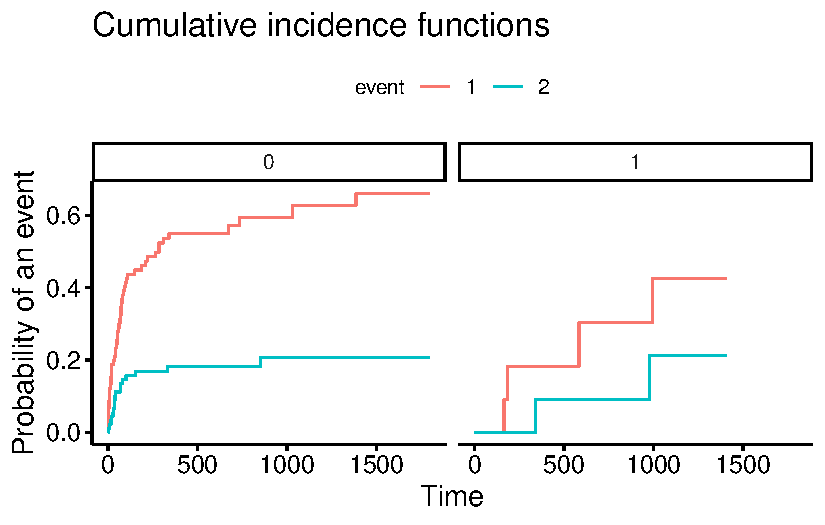
\includegraphics{14-R_files/figure-pdf/unnamed-chunk-42-1.pdf}

}

\end{figure}

Avec \texttt{survminer}

\begin{Shaded}
\begin{Highlighting}[]
\FunctionTok{ggcompetingrisks}\NormalTok{(}\AttributeTok{fit =}\NormalTok{ ic)}
\end{Highlighting}
\end{Shaded}

\begin{figure}[H]

{\centering 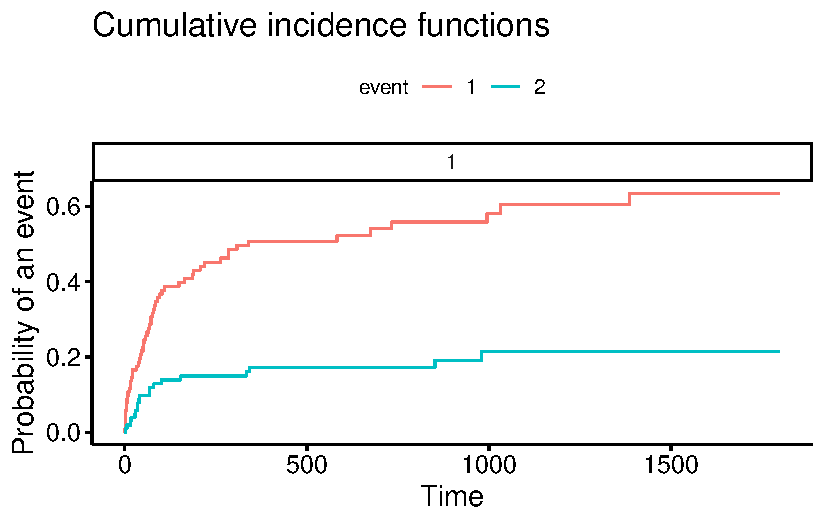
\includegraphics{14-R_files/figure-pdf/unnamed-chunk-43-1.pdf}

}

\end{figure}

\emph{Comparaison de groupes}

Le test de Gray est automatiquement exécuté.

\begin{Shaded}
\begin{Highlighting}[]
\NormalTok{ic }\OtherTok{=} \FunctionTok{cuminc}\NormalTok{(compet}\SpecialCharTok{$}\NormalTok{stime, compet}\SpecialCharTok{$}\NormalTok{compet, }\AttributeTok{group=}\NormalTok{compet}\SpecialCharTok{$}\NormalTok{surgery, }\AttributeTok{rho=}\DecValTok{1}\NormalTok{)}
\NormalTok{ic }
\end{Highlighting}
\end{Shaded}

\begin{verbatim}
Tests:
      stat         pv df
1 4.604792 0.03188272  1
2 0.272147 0.60189515  1
Estimates and Variances:
$est
           500      1000      1500
0 1 0.54917896 0.5940358 0.6604903
1 1 0.18181818 0.4242424        NA
0 2 0.18168014 0.2066006 0.2066006
1 2 0.09090909 0.2121212        NA

$var
            500        1000        1500
0 1 0.002955869 0.003335897 0.004199157
1 1 0.014958678 0.033339569          NA
0 2 0.001727112 0.002271242 0.002271242
1 2 0.008449138 0.022024737          NA
\end{verbatim}

\begin{Shaded}
\begin{Highlighting}[]
\FunctionTok{plot}\NormalTok{(ic)}
\end{Highlighting}
\end{Shaded}

\begin{figure}[H]

{\centering 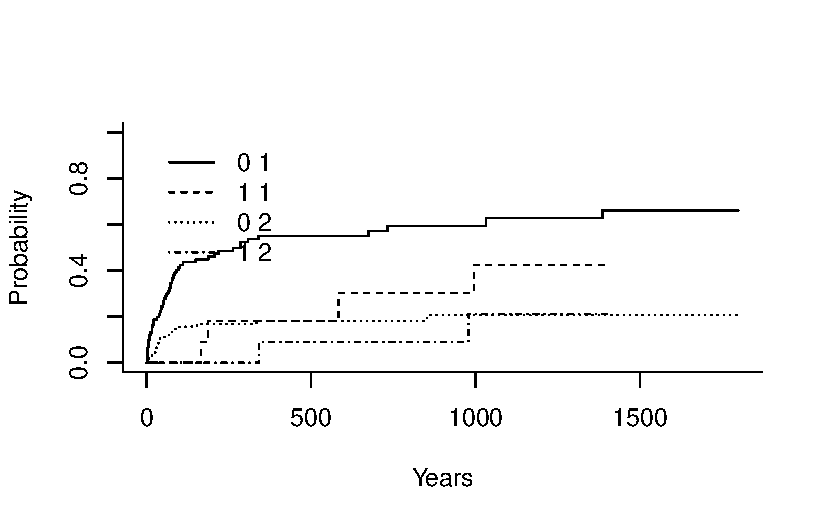
\includegraphics{14-R_files/figure-pdf/unnamed-chunk-44-1.pdf}

}

\end{figure}

Avec \texttt{survminer}, pour obtenir un seul graphique pour toutes les
courbes ajouter l'option \textbf{\texttt{multiple\_panels\ =\ F}}

\begin{Shaded}
\begin{Highlighting}[]
\FunctionTok{ggcompetingrisks}\NormalTok{(}\AttributeTok{fit =}\NormalTok{ ic)}
\end{Highlighting}
\end{Shaded}

\begin{figure}[H]

{\centering 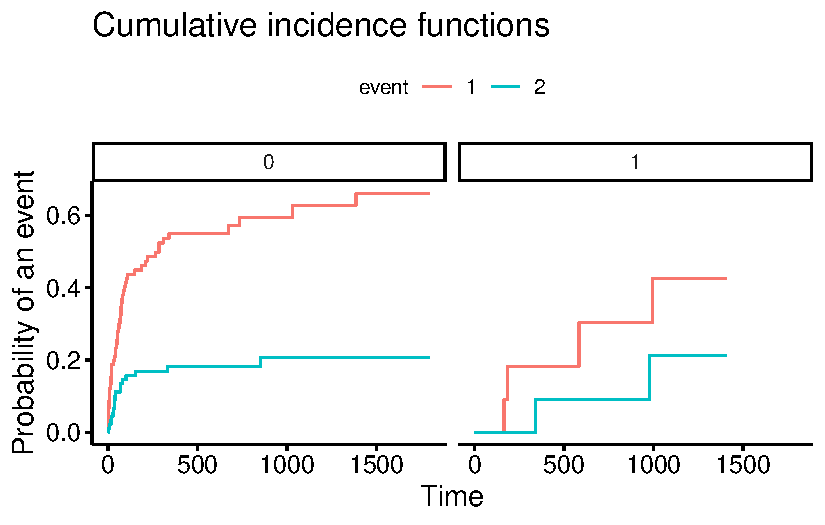
\includegraphics{14-R_files/figure-pdf/unnamed-chunk-45-1.pdf}

}

\end{figure}

\begin{Shaded}
\begin{Highlighting}[]
\FunctionTok{ggcompetingrisks}\NormalTok{(}\AttributeTok{fit =}\NormalTok{ ic, }\AttributeTok{multiple\_panels =}\NormalTok{ F)}
\end{Highlighting}
\end{Shaded}

\begin{figure}[H]

{\centering 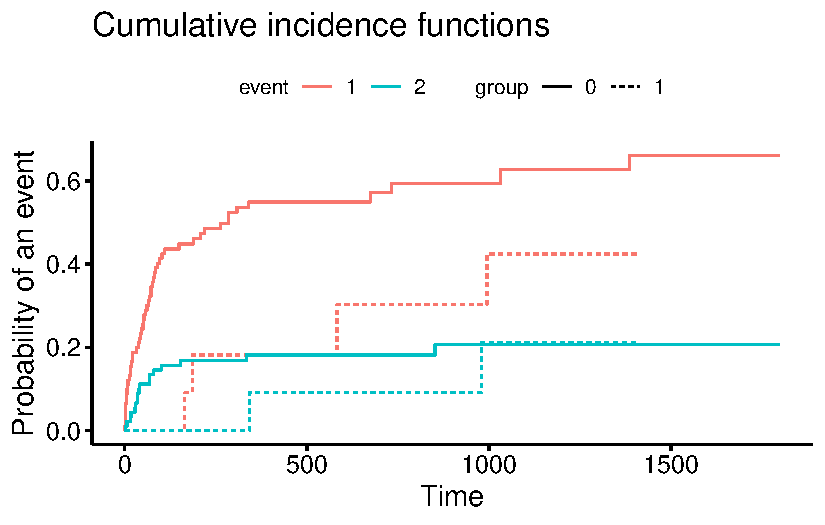
\includegraphics{14-R_files/figure-pdf/unnamed-chunk-45-2.pdf}

}

\end{figure}

\hypertarget{moduxe8les-1}{%
\subsubsection{\texorpdfstring{\textbf{Modèles}}{Modèles}}\label{moduxe8les-1}}

On va utilisé seulement le modèle multinomial à durée discrète, le
modèle \emph{fine-gray} pendant du modèle de Cox pour les risques
concurrents étant fortement critiqué. Si une analyse de type
\emph{cause-specific} est envisageable (issues concurrentes traitées
comme des censures à droites) on utilise simplement la fonction
\texttt{coxph} de \texttt{survival}.

On va de nouveau utiliser la variable mois (durée discrète). Le modèle
sera estimé à l'aide la fonction \textbf{\texttt{multinom}} du très
vieillissant package \texttt{nnet}, les p-values doivent-être
programmées, l'output ne donnant que les erreurs-types.

\emph{Mise en formae de la base}

\begin{Shaded}
\begin{Highlighting}[]
\NormalTok{compet }\OtherTok{\textless{}{-}} \FunctionTok{read.csv}\NormalTok{(}\StringTok{"https://raw.githubusercontent.com/mthevenin/analyse\_duree/master/bases/transplantation.csv"}\NormalTok{)}

\NormalTok{compet}\SpecialCharTok{$}\NormalTok{T }\OtherTok{=}\NormalTok{ compet}\SpecialCharTok{$}\NormalTok{mois}
\NormalTok{td }\OtherTok{=} \FunctionTok{uncount}\NormalTok{(compet, mois)}
\NormalTok{td }\OtherTok{=} \FunctionTok{arrange}\NormalTok{(td, id)}

\NormalTok{td}\SpecialCharTok{$}\NormalTok{x}\OtherTok{=}\DecValTok{1}
\NormalTok{td}\SpecialCharTok{$}\NormalTok{t }\OtherTok{=} \FunctionTok{ave}\NormalTok{(td}\SpecialCharTok{$}\NormalTok{x, td}\SpecialCharTok{$}\NormalTok{id, }\AttributeTok{FUN=}\NormalTok{cumsum)}
\NormalTok{td}\SpecialCharTok{$}\NormalTok{t2 }\OtherTok{=}\NormalTok{ td}\SpecialCharTok{$}\NormalTok{t}\SpecialCharTok{\^{}}\DecValTok{2}

\NormalTok{my }\OtherTok{=} \FunctionTok{mean}\NormalTok{(td}\SpecialCharTok{$}\NormalTok{year)}
\NormalTok{td}\SpecialCharTok{$}\NormalTok{yearb }\OtherTok{=}\NormalTok{ td}\SpecialCharTok{$}\NormalTok{year }\SpecialCharTok{{-}}\NormalTok{ my}
\NormalTok{ma }\OtherTok{=} \FunctionTok{mean}\NormalTok{(td}\SpecialCharTok{$}\NormalTok{age)}
\NormalTok{td}\SpecialCharTok{$}\NormalTok{ageb }\OtherTok{=}\NormalTok{ td}\SpecialCharTok{$}\NormalTok{age  }\SpecialCharTok{{-}}\NormalTok{ ma}

\NormalTok{td}\SpecialCharTok{$}\NormalTok{e }\OtherTok{=} \FunctionTok{ifelse}\NormalTok{(td}\SpecialCharTok{$}\NormalTok{t}\SpecialCharTok{\textless{}}\NormalTok{td}\SpecialCharTok{$}\NormalTok{T,}\DecValTok{0}\NormalTok{, td}\SpecialCharTok{$}\NormalTok{compet)}
\end{Highlighting}
\end{Shaded}

\emph{Estimation}

Pour estimer le modèle, on utilise la fonction \textbf{\texttt{mlogit}}.
Les p-values seront calculées à partir d'un test bilatéral (statistique
z).

\begin{Shaded}
\begin{Highlighting}[]
\NormalTok{competfit }\OtherTok{=} \FunctionTok{multinom}\NormalTok{(}\AttributeTok{formula =}\NormalTok{ e }\SpecialCharTok{\textasciitilde{}}\NormalTok{ t }\SpecialCharTok{+}\NormalTok{ t2 }\SpecialCharTok{+}\NormalTok{ yearb }\SpecialCharTok{+}\NormalTok{ ageb }\SpecialCharTok{+}\NormalTok{ surgery, }\AttributeTok{data =}\NormalTok{ td)}
\end{Highlighting}
\end{Shaded}

\begin{verbatim}
# weights:  21 (12 variable)
initial  value 1238.136049 
iter  10 value 608.949443
iter  20 value 341.102661
iter  30 value 277.143136
iter  40 value 275.005451
final  value 275.005419 
converged
\end{verbatim}

\begin{Shaded}
\begin{Highlighting}[]
\FunctionTok{tbl\_regression}\NormalTok{(competfit, }\AttributeTok{exponentiate =} \ConstantTok{TRUE}\NormalTok{,)}
\end{Highlighting}
\end{Shaded}

\begin{longtable}[]{@{}llccc@{}}
\toprule\noalign{}
\textbf{Outcome} & \textbf{Characteristic} & \textbf{OR} & \textbf{95\%
CI} & \textbf{p-value} \\
\midrule\noalign{}
\endhead
\bottomrule\noalign{}
\endlastfoot
1 & t & 0.82 & 0.75, 0.88 & \textless0.001 \\
& t2 & 1.00 & 1.00, 1.00 & \textless0.001 \\
& yearb & 0.88 & 0.75, 1.03 & 0.12 \\
& ageb & 1.04 & 1.01, 1.08 & 0.012 \\
& surgery & 0.32 & 0.11, 0.91 & 0.033 \\
2 & t & 0.82 & 0.71, 0.94 & 0.003 \\
& t2 & 1.00 & 1.00, 1.01 & 0.052 \\
& yearb & 0.82 & 0.62, 1.07 & 0.14 \\
& ageb & 1.01 & 0.96, 1.06 & 0.7 \\
& surgery & 0.54 & 0.12, 2.50 & 0.4 \\
\end{longtable}

\hypertarget{stata-6}{%
\chapter{\texorpdfstring{\textbf{Stata}}{Stata}}\label{stata-6}}

\begin{tcolorbox}[enhanced jigsaw, arc=.35mm, bottomrule=.15mm, titlerule=0mm, colbacktitle=quarto-callout-note-color!10!white, left=2mm, opacitybacktitle=0.6, toprule=.15mm, title=\textcolor{quarto-callout-note-color}{\faInfo}\hspace{0.5em}{Note}, colframe=quarto-callout-note-color-frame, breakable, coltitle=black, opacityback=0, toptitle=1mm, bottomtitle=1mm, rightrule=.15mm, leftrule=.75mm, colback=white]

\begin{itemize}
\tightlist
\item
  Le document a été compilé avec le magique kernel jupyter
  \href{https://github.com/hugetim/nbstata}{\textbf{nbstata}} programmé
  par \textbf{Tim Huegerich}. Comparé à l'ancienne solution
  \textbf{statamarkdown} qui exécutait Stata en mode batch, il n'y a pas
  photo au niveau du runtime, avec pratiquement aucune latence une fois
  le noyau chargé (attendre une quinzaine de seconde à la première
  compilation).
\item
  Le document n'a pas été compilé en PDF, seule cette version html est
  disponible.
\end{itemize}

\end{tcolorbox}

Ouverture de la base

\begin{verbatim}
<IPython.core.display.HTML object>
\end{verbatim}

\begin{verbatim}
(prefix now "https://raw.githubusercontent.com//mthevenin/analyse_duree/master/
> bases")
\end{verbatim}

\begin{verbatim}
(SAVASTATA created this dataset on 01AUG2019)
(prefix now "https://www.stata-press.com/data/r18")

     +------------------------------------------+
     | id   year   age   surgery   stime   died |
     |------------------------------------------|
  1. | 15     68    53         0       1      1 |
  2. | 43     70    43         0       2      1 |
  3. | 61     71    52         0       2      1 |
  4. | 75     72    52         0       2      1 |
  5. |  6     68    54         0       3      1 |
     |------------------------------------------|
  6. | 42     70    36         0       3      1 |
  7. | 54     71    47         0       3      1 |
  8. | 38     70    41         0       5      1 |
  9. | 85     73    47         0       5      1 |
 10. |  2     68    51         0       6      1 |
     +------------------------------------------+
\end{verbatim}

\hypertarget{analyse-non-paramuxe9trique-1}{%
\section{Analyse non paramétrique}\label{analyse-non-paramuxe9trique-1}}

\hypertarget{muxe9thode-actuarielle-1}{%
\subsection{Méthode actuarielle}\label{muxe9thode-actuarielle-1}}

Contrairement à la formation, l'estimation sera faite sur des
intervalles de 30 jours

\begin{Shaded}
\begin{Highlighting}[]
\KeywordTok{ltable}\NormalTok{ stime died, interval(30) }\KeywordTok{graph} \KeywordTok{ci}
\end{Highlighting}
\end{Shaded}

\begin{verbatim}

                 Beg.                                 Std.
   Interval     total   Deaths   Lost   Survival     error     [95% conf. int.]
-------------------------------------------------------------------------------
    0    30       103       22      1     0.7854    0.0406     0.6926    0.8531
   30    60        80       14      2     0.6462    0.0475     0.5449    0.7305
   60    90        64       12      0     0.5250    0.0498     0.4232    0.6171
   90   120        52        5      1     0.4741    0.0499     0.3738    0.5677
  120   150        46        1      1     0.4636    0.0499     0.3637    0.5575
  150   180        44        2      0     0.4426    0.0498     0.3435    0.5369
  180   210        42        3      1     0.4106    0.0495     0.3132    0.5053
  210   240        38        1      0     0.3998    0.0494     0.3030    0.4945
  240   270        37        1      1     0.3888    0.0492     0.2928    0.4836
  270   300        35        2      0     0.3666    0.0488     0.2720    0.4614
  300   330        33        1      0     0.3555    0.0486     0.2618    0.4502
  330   360        32        3      1     0.3216    0.0478     0.2308    0.4157
  360   390        28        0      1     0.3216    0.0478     0.2308    0.4157
  390   420        27        0      1     0.3216    0.0478     0.2308    0.4157
  420   450        26        0      2     0.3216    0.0478     0.2308    0.4157
  480   510        24        0      1     0.3216    0.0478     0.2308    0.4157
  510   540        23        0      1     0.3216    0.0478     0.2308    0.4157
  540   570        22        0      1     0.3216    0.0478     0.2308    0.4157
  570   600        21        1      1     0.3059    0.0479     0.2155    0.4010
  600   630        19        0      1     0.3059    0.0479     0.2155    0.4010
  660   690        18        1      1     0.2885    0.0483     0.1982    0.3849
  720   750        16        1      0     0.2704    0.0485     0.1807    0.3681
  840   870        15        1      1     0.2518    0.0486     0.1629    0.3506
  900   930        13        0      1     0.2518    0.0486     0.1629    0.3506
  930   960        12        0      1     0.2518    0.0486     0.1629    0.3506
  960   990        11        1      0     0.2289    0.0493     0.1404    0.3304
  990  1020        10        1      0     0.2060    0.0494     0.1192    0.3093
 1020  1050         9        1      0     0.1831    0.0489     0.0992    0.2873
 1140  1170         8        0      1     0.1831    0.0489     0.0992    0.2873
 1320  1350         7        0      1     0.1831    0.0489     0.0992    0.2873
 1380  1410         6        1      2     0.1465    0.0510     0.0645    0.2602
 1560  1590         3        0      2     0.1465    0.0510     0.0645    0.2602
 1770  1800         1        0      1     0.1465    0.0510     0.0645    0.2602
-------------------------------------------------------------------------------
\end{verbatim}

\begin{figure}[H]

{\centering 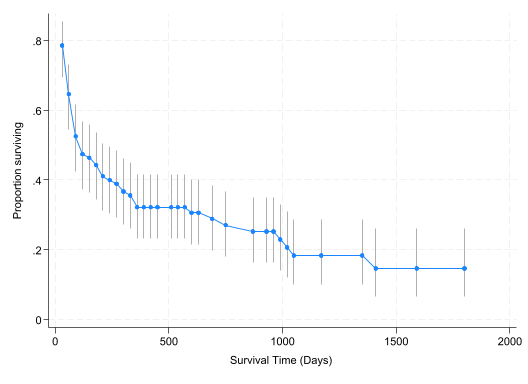
\includegraphics{15-Stata_files/figure-pdf/cell-3-output-2.png}

}

\end{figure}

\textbf{Récupération des quartiles de la durée}

Installation de la commande \texttt{qlt}

\begin{Shaded}
\begin{Highlighting}[]
\NormalTok{net install qlt, from(}\StringTok{"https://raw.githubusercontent.com/mthevenin/analyse\_duree/master/ado/qlt/"}\NormalTok{) }\KeywordTok{replace}

\NormalTok{* }\KeywordTok{help}\NormalTok{ qlt}
\end{Highlighting}
\end{Shaded}

\begin{Shaded}
\begin{Highlighting}[]
\KeywordTok{qui} \KeywordTok{ltable}\NormalTok{ stime died, interval(30) }\KeywordTok{saving}\NormalTok{(base, }\KeywordTok{replace}\NormalTok{)}
\KeywordTok{use}\NormalTok{ base, }\KeywordTok{clear}
\end{Highlighting}
\end{Shaded}

\begin{verbatim}
(SAVASTATA created this dataset on 01AUG2019)
\end{verbatim}

\begin{Shaded}
\begin{Highlighting}[]
\NormalTok{qlt}
\end{Highlighting}
\end{Shaded}

\begin{verbatim}
Duree pour differents quantiles de la fonction de survie
Definition des bornes Stata-ltable
S(t)=0.90: t=        .
S(t)=0.75: t=    7.623
S(t)=0.50: t=   74.729
S(t)=0.25: t=  849.325
S(t)=0.10: t=        .
\end{verbatim}

Avec la définition des bornes des intervalles de Sas

\begin{Shaded}
\begin{Highlighting}[]
\NormalTok{qlt, sas}
\end{Highlighting}
\end{Shaded}

\begin{verbatim}
Duree pour differents quantiles de la fonction de survie
Definition des bornes Sas-lifetest
\end{verbatim}

\begin{verbatim}
S(t)=0.90: t=   13.977
\end{verbatim}

\begin{verbatim}
S(t)=0.75: t=   37.623
S(t)=0.50: t=  104.729
S(t)=0.25: t=  906.993
S(t)=0.10: t=        .
\end{verbatim}

\hypertarget{muxe9thode-kaplan-meier-1}{%
\subsection{Méthode Kaplan-Meier}\label{muxe9thode-kaplan-meier-1}}

\textbf{Mode analyse des durées: stset}

Les données doivent être mises en mode analyse de durée avec la commande
\texttt{stset} (\texttt{help\ stset}).

A minima la commande \texttt{stset} entre la variable de durée en
argument principal et la variable de censure/évènement avec
\texttt{failure(nom\_var)} en option.

\begin{Shaded}
\begin{Highlighting}[]
\KeywordTok{stset}\NormalTok{ stime, f(died)}

\OtherTok{list}\NormalTok{ id stime died \_st \_d \_t \_t0 }\KeywordTok{in}\NormalTok{ 1/10}
\end{Highlighting}
\end{Shaded}

\begin{verbatim}

Survival-time data settings

         Failure event: died!=0 & died<.
Observed time interval: (0, stime]
     Exit on or before: failure

--------------------------------------------------------------------------
        103  total observations
          0  exclusions
--------------------------------------------------------------------------
        103  observations remaining, representing
         75  failures in single-record/single-failure data
     31,938  total analysis time at risk and under observation
                                                At risk from t =         0
                                     Earliest observed entry t =         0
                                          Last observed exit t =     1,799

     +-----------------------------------------+
     | id   stime   died   _st   _d   _t   _t0 |
     |-----------------------------------------|
  1. | 15       1      1     1    1    1     0 |
  2. | 43       2      1     1    1    2     0 |
  3. | 61       2      1     1    1    2     0 |
  4. | 75       2      1     1    1    2     0 |
  5. |  6       3      1     1    1    3     0 |
     |-----------------------------------------|
  6. | 42       3      1     1    1    3     0 |
  7. | 54       3      1     1    1    3     0 |
\end{verbatim}

\begin{verbatim}
  8. | 38       5      1     1    1    5     0 |
  9. | 85       5      1     1    1    5     0 |
 10. |  2       6      1     1    1    6     0 |
     +-----------------------------------------+
\end{verbatim}

\textbf{Estimation de la fonction de survie}

La commande \texttt{sts\ list} permet d'afficher le tableau des
estimations à chaque moment d'évènement

\begin{tcolorbox}[enhanced jigsaw, arc=.35mm, bottomrule=.15mm, titlerule=0mm, colbacktitle=quarto-callout-note-color!10!white, left=2mm, opacitybacktitle=0.6, toprule=.15mm, title=\textcolor{quarto-callout-note-color}{\faInfo}\hspace{0.5em}{Note}, colframe=quarto-callout-note-color-frame, breakable, coltitle=black, opacityback=0, toptitle=1mm, bottomtitle=1mm, rightrule=.15mm, leftrule=.75mm, colback=white]

Le tableau des estimateurs n'est reporté que pour le format htl du
support

\end{tcolorbox}

On récupére les quantiles de la durée avec \texttt{stci}. Par défaut la
commande affiche la durée médiane. On peut choisir le quantile avec
l'arguement p(valeur) en option

\begin{Shaded}
\begin{Highlighting}[]
\KeywordTok{stci}

\KeywordTok{stci}\NormalTok{, }\KeywordTok{p}\NormalTok{(75)}
\KeywordTok{stci}\NormalTok{, }\KeywordTok{p}\NormalTok{(25)}
\end{Highlighting}
\end{Shaded}

\begin{verbatim}

        Failure _d: died
  Analysis time _t: stime

             | Number of 
             |  subjects         50%      Std. err.    [95% conf. interval]
-------------+-------------------------------------------------------------
\end{verbatim}

\begin{verbatim}
       Total |       103         100      38.64425           69        219

        Failure _d: died
  Analysis time _t: stime

             | Number of 
             |  subjects         75%      Std. err.    [95% conf. interval]
-------------+-------------------------------------------------------------
\end{verbatim}

\begin{verbatim}
       Total |       103         979      144.4728          340          .
\end{verbatim}

\begin{verbatim}

        Failure _d: died
  Analysis time _t: stime

             | Number of 
             |  subjects         25%      Std. err.    [95% conf. interval]
-------------+-------------------------------------------------------------
\end{verbatim}

\begin{verbatim}
       Total |       103          36      9.033439           16         51
\end{verbatim}

Pour afficher le graphique des estimateurs KM, on utilise la commande
\textbf{\texttt{sts\ graph}}. On ajoute ici l'affichage des intervalles
de confiance avec l'option \texttt{ci}

\begin{Shaded}
\begin{Highlighting}[]
\KeywordTok{sts} \KeywordTok{graph}\NormalTok{, }\KeywordTok{ci}
\end{Highlighting}
\end{Shaded}

\begin{verbatim}

        Failure _d: died
  Analysis time _t: stime
\end{verbatim}

\begin{figure}[H]

{\centering 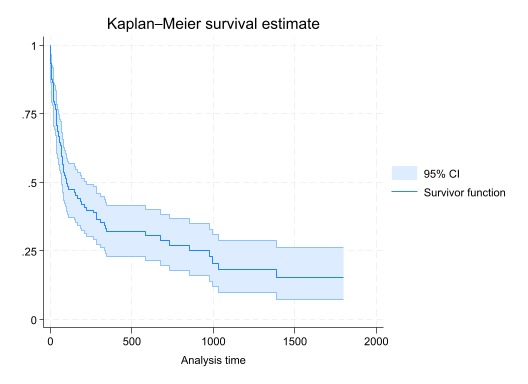
\includegraphics{15-Stata_files/figure-pdf/cell-12-output-2.png}

}

\end{figure}

Les commandes \texttt{sts\ list}, \texttt{stci} et \texttt{sts\ graph}
permettent avec l'option \texttt{by(nom\_variable)} d'obtenir des
comparaisons entre groupes.

\hypertarget{comparaison-des-fonctions-de-survie-km}{%
\subsection{Comparaison des fonctions de survie
(KM)}\label{comparaison-des-fonctions-de-survie-km}}

On va comparer les fonctions de survie pour la variable \emph{surgery}.

\textbf{Graphique}

On ajoute l'option \texttt{by(surgery)} à la commande
\texttt{sts\ graph}

\begin{Shaded}
\begin{Highlighting}[]
\KeywordTok{sts} \KeywordTok{graph}\NormalTok{, }\KeywordTok{by}\NormalTok{(surgery) }\KeywordTok{ci}\NormalTok{ ci1opts(fc(stc1\%40))  ci2opts(fc(stc2\%40)) }\BaseNTok{legend}\NormalTok{(pos(6))}
\end{Highlighting}
\end{Shaded}

\begin{verbatim}

        Failure _d: died
  Analysis time _t: stime
\end{verbatim}

\begin{figure}[H]

{\centering 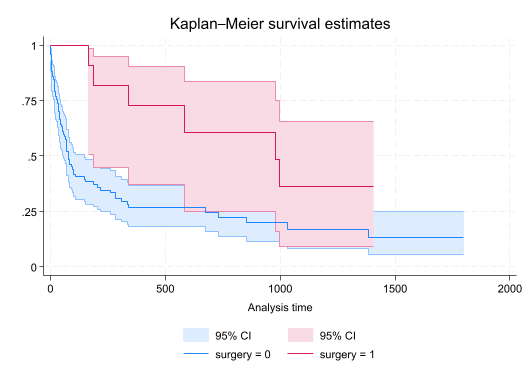
\includegraphics{15-Stata_files/figure-pdf/cell-13-output-2.png}

}

\end{figure}

\textbf{Tests du logrank}

Fonction \textbf{\texttt{sts\ test}}. On affichera ici plusieurs
variantes du test.

\begin{Shaded}
\begin{Highlighting}[]
\KeywordTok{local} \KeywordTok{test} \StringTok{\textasciigrave{}"} \StringTok{"l"} \StringTok{"w"} \StringTok{"tw"} \StringTok{"p"} \StringTok{"\textquotesingle{}}
\StringTok{foreach test2 of local test \{}
\StringTok{sts test surgery, \textasciigrave{}test2\textquotesingle{}}
\StringTok{\}}
\end{Highlighting}
\end{Shaded}

\begin{verbatim}

        Failure _d: died
  Analysis time _t: stime

Equality of survivor functions
Log-rank test

        |  Observed       Expected
surgery |    events         events
--------+-------------------------
      0 |        69          60.34
      1 |         6          14.66
--------+-------------------------
  Total |        75          75.00

                  chi2(1) =   6.59
                  Pr>chi2 = 0.0103

        Failure _d: died
  Analysis time _t: stime
\end{verbatim}

\begin{verbatim}

Equality of survivor functions
Wilcoxon–Breslow–Gehan test

        |  Observed       Expected       Sum of
surgery |    events         events        ranks
--------+--------------------------------------
      0 |        69          60.34          623
      1 |         6          14.66         -623
--------+--------------------------------------
  Total |        75          75.00            0

                               chi2(1) =   8.99
                               Pr>chi2 = 0.0027

        Failure _d: died
  Analysis time _t: stime
\end{verbatim}

\begin{verbatim}

Equality of survivor functions
Tarone–Ware test

        |  Observed       Expected       Sum of
surgery |    events         events        ranks
--------+--------------------------------------
      0 |        69          60.34    73.105398
      1 |         6          14.66   -73.105398
--------+--------------------------------------
  Total |        75          75.00            0

                               chi2(1) =   8.46
                               Pr>chi2 = 0.0036

        Failure _d: died
  Analysis time _t: stime
\end{verbatim}

\begin{verbatim}

Equality of survivor functions
Peto–Peto–Prentice test

        |  Observed       Expected       Sum of
surgery |    events         events        ranks
--------+--------------------------------------
      0 |        69          60.34    6.0505875
      1 |         6          14.66   -6.0505875
--------+--------------------------------------
  Total |        75          75.00            0

                               chi2(1) =   8.66
                               Pr>chi2 = 0.0032
\end{verbatim}

\emph{Comparaison des rmst}

Installation de la commande \textbf{\texttt{strmst2}}

\begin{Shaded}
\begin{Highlighting}[]
\KeywordTok{ssc}\NormalTok{ install strmst2}
\end{Highlighting}
\end{Shaded}

\begin{itemize}
\tightlist
\item
  Comparaison deux à deux (c'est pas plus mal comme cela). Je conseille
  de mettre les variables sous forme d'indicatrice.
\item
  Les labels de la variable ne sont jamais reportés. Ils sont remplacés
  par les modalités arm0 et arm1.
\item
  On peut changer la valeurs maximale de la durée avec l'option
  \texttt{tau(valeur)}.
\end{itemize}

arm1 = Opération\\
arm0 = pas d'opération

\begin{Shaded}
\begin{Highlighting}[]
\NormalTok{strmst2 surgery}
\end{Highlighting}
\end{Shaded}

\begin{verbatim}
 
Number of observations for analysis = 103
 
The truncation time, tau, was not specified. Thus, the default tau (the minimum
>  of the
largest observed event time within each group), 995.000, is used.
\end{verbatim}

\begin{verbatim}

Restricted Mean Survival Time (RMST) by arm
-----------------------------------------------------------
   Group |  Estimate    Std. Err.      [95% Conf. Interval]
---------+-------------------------------------------------
   arm 1 |   734.758     104.187      530.554      938.961
   arm 0 |   310.168      42.481      226.907      393.429
-----------------------------------------------------------

Between-group contrast (arm 1 versus arm 0) 
------------------------------------------------------------------------
           Contrast  |  Estimate       [95% Conf. Interval]     P>|z|
---------------------+--------------------------------------------------
RMST (arm 1 - arm 0) |   424.590      204.064      645.115      0.000
RMST (arm 1 / arm 0) |     2.369        1.610        3.486      0.000
------------------------------------------------------------------------
\end{verbatim}

\hypertarget{moduxe8les-uxe0-risques-proportionnels-1}{%
\section{Modèles à risques
proportionnels}\label{moduxe8les-uxe0-risques-proportionnels-1}}

\hypertarget{moduxe8le-de-cox-2}{%
\subsection{Modèle de Cox}\label{moduxe8le-de-cox-2}}

\hypertarget{estimation-du-moduxe8le-1}{%
\subsubsection{Estimation du modèle}\label{estimation-du-moduxe8le-1}}

Commande \textbf{\texttt{stcox}}

Avec la correction d'Efron (conseillé)

\textbf{HR}:

\begin{Shaded}
\begin{Highlighting}[]
\KeywordTok{stcox} \FunctionTok{year}\NormalTok{ age surgery, }\KeywordTok{nolog}\NormalTok{ noshow efron}
\end{Highlighting}
\end{Shaded}

\begin{verbatim}

Cox regression with Efron method for ties

No. of subjects =    103                                Number of obs =    103
No. of failures =     75
Time at risk    = 31,938
                                                        LR chi2(3)    =  17.63
Log likelihood = -289.30639                             Prob > chi2   = 0.0005
\end{verbatim}

\begin{verbatim}
------------------------------------------------------------------------------
\end{verbatim}

\begin{verbatim}
          _t | Haz. ratio   Std. err.      z    P>|z|     [95% conf. interval]
\end{verbatim}

\begin{verbatim}
-------------+----------------------------------------------------------------
\end{verbatim}

\begin{verbatim}
        year |
\end{verbatim}

\begin{verbatim}
      0.887      0.060    -1.78   0.076        0.778       1.012
         age |      1.030      0.014     2.19   0.029        1.003       1.058
     surgery |      0.373      0.163    -2.26   0.024        0.158       0.876
\end{verbatim}

\begin{verbatim}
------------------------------------------------------------------------------
\end{verbatim}

\textbf{log(HR)}:

\begin{Shaded}
\begin{Highlighting}[]
\KeywordTok{stcox} \FunctionTok{year}\NormalTok{ age surgery, }\KeywordTok{nolog}\NormalTok{ noshow efron nohr}
\end{Highlighting}
\end{Shaded}

\begin{verbatim}

Cox regression with Efron method for ties

No. of subjects =    103                                Number of obs =    103
No. of failures =     75
Time at risk    = 31,938
                                                        LR chi2(3)    =  17.63
Log likelihood = -289.30639                             Prob > chi2   = 0.0005

------------------------------------------------------------------------------
          _t | Coefficient  Std. err.      z    P>|z|     [95% conf. interval]
\end{verbatim}

\begin{verbatim}
-------------+----------------------------------------------------------------
        year |     -0.120      0.067    -1.78   0.076       -0.252       0.012
         age |      0.030      0.014     2.19   0.029        0.003       0.056
     surgery |     -0.987      0.436    -2.26   0.024       -1.842      -0.132
------------------------------------------------------------------------------
\end{verbatim}

\hypertarget{test-de-lhypothuxe8se-ph}{%
\subsubsection{Test de l'hypothèse PH}\label{test-de-lhypothuxe8se-ph}}

\textbf{Test Grambsch-Therneau sur les résidus de Schoenfeld}

Le test OLS est exécuté avec la commande
\textbf{\texttt{estat\ phtest}}. Je conseille d'ajouté l'option detail
pour récupéré les test à un degré de liberté, le test omnibus n'étant
pas fiable.

Par défaut \(f(t)=t\).

\begin{Shaded}
\begin{Highlighting}[]
\NormalTok{* f(t)=t {-} par défaut }

\KeywordTok{estat}\NormalTok{ phtest, }\KeywordTok{detail}


\NormalTok{* f(t)= 1{-}km {-} solution par défaut }\KeywordTok{de}\NormalTok{ R}
      
\KeywordTok{estat}\NormalTok{ phtest, }\KeywordTok{detail}\NormalTok{ km}
\end{Highlighting}
\end{Shaded}

\begin{verbatim}

Test of proportional-hazards assumption

Time function: Analysis time
--------------------------------------------------------
             |        rho     chi2       df    Prob>chi2
-------------+------------------------------------------
        year |    0.10162     0.80        1       0.3720
\end{verbatim}

\begin{verbatim}
         age |    0.12937     1.61        1       0.2043
     surgery |    0.29664     5.54        1       0.0186
-------------+------------------------------------------
 Global test |                8.76        3       0.0327
--------------------------------------------------------

Test of proportional-hazards assumption

Time function: 1 - Kaplan–Meier estimate
--------------------------------------------------------
             |        rho     chi2       df    Prob>chi2
-------------+------------------------------------------
        year |    0.15920     1.96        1       0.1620
         age |    0.10907     1.15        1       0.2845
     surgery |    0.25096     3.96        1       0.0465
-------------+------------------------------------------
 Global test |                7.99        3       0.0462
--------------------------------------------------------
\end{verbatim}

\textbf{Intéraction avec une fonction de la durée}

Avec \(f(t)=t\)

L'intéraction s'ajoute directement en option en indiquant la ou les
variables concernées (une seule de préférence) avec l'option
\texttt{tvc(nom\_variable)} et la transformation de la durée (variable
\emph{t}) avec l'option \texttt{texp(expression)}. Ici on a choisi
\(ft(t)\) soit l'expression dans l'option \texttt{texp(\_t)}

\begin{Shaded}
\begin{Highlighting}[]
\KeywordTok{stcox} \FunctionTok{year}\NormalTok{ age surgery, }\KeywordTok{nolog}\NormalTok{ noshow efron nohr tvc(surgery) texp(\_t)}
\end{Highlighting}
\end{Shaded}

\begin{verbatim}


Cox regression with Efron method for ties

No. of subjects =    103                                Number of obs =    103
No. of failures =     75
Time at risk    = 31,938
                                                        LR chi2(4)    =  21.58
Log likelihood = -287.32903                             Prob > chi2   = 0.0002

------------------------------------------------------------------------------
          _t | Coefficient  Std. err.      z    P>|z|     [95% conf. interval]
-------------+----------------------------------------------------------------
main         |
\end{verbatim}

\begin{verbatim}
        year |     -0.123      0.067    -1.84   0.066       -0.254       0.008
         age |      0.029      0.013     2.15   0.032        0.003       0.055
     surgery |     -1.755      0.674    -2.60   0.009       -3.077      -0.433
-------------+----------------------------------------------------------------
tvc          |
     surgery |      0.002      0.001     2.02   0.043        0.000       0.004
------------------------------------------------------------------------------
Note: Variables in tvc equation interacted with _t.
\end{verbatim}

\hypertarget{introduction-dune-variable-dynamique-binaire-1}{%
\subsubsection{Introduction d'une variable dynamique
(binaire)}\label{introduction-dune-variable-dynamique-binaire-1}}

\textbf{Transformation de la base en format long aux temps d'évènement}

\emph{Etape 1}

\begin{Shaded}
\begin{Highlighting}[]
\KeywordTok{stset}\NormalTok{ stime, f(died) id(id)}
\end{Highlighting}
\end{Shaded}

\begin{verbatim}

Survival-time data settings

           ID variable: id
         Failure event: died!=0 & died<.
Observed time interval: (stime[_n-1], stime]
     Exit on or before: failure

--------------------------------------------------------------------------
        103  total observations
          0  exclusions
--------------------------------------------------------------------------
        103  observations remaining, representing
        103  subjects
         75  failures in single-failure-per-subject data
     31,938  total analysis time at risk and under observation
                                                At risk from t =         0
                                     Earliest observed entry t =         0
                                          Last observed exit t =     1,799
\end{verbatim}

\emph{Etape 2}

\begin{Shaded}
\begin{Highlighting}[]
\KeywordTok{stsplit}\NormalTok{, }\FunctionTok{at}\NormalTok{(failure)}

\KeywordTok{stset}\NormalTok{ stime, f(died) id(id)}
\end{Highlighting}
\end{Shaded}

\begin{verbatim}
(62 failure times)
\end{verbatim}

\begin{verbatim}
(3,470 observations (episodes) created)
\end{verbatim}

\begin{verbatim}

Survival-time data settings

           ID variable: id
         Failure event: died!=0 & died<.
Observed time interval: (stime[_n-1], stime]
     Exit on or before: failure

--------------------------------------------------------------------------
      3,573  total observations
          0  exclusions
--------------------------------------------------------------------------
      3,573  observations remaining, representing
        103  subjects
         75  failures in single-failure-per-subject data
\end{verbatim}

\begin{verbatim}
     31,938  total analysis time at risk and under observation
                                                At risk from t =         0
                                     Earliest observed entry t =         0
                                          Last observed exit t =     1,799
\end{verbatim}

\emph{Etape 3}

\begin{Shaded}
\begin{Highlighting}[]
\KeywordTok{gen}\NormalTok{ tvc = transplant==1 \& wait\textless{}=\_t}
\KeywordTok{sort}\NormalTok{ id \_t}
\OtherTok{list}\NormalTok{ id transplant wait tvc \_d \_t \_t0 }\KeywordTok{if}\NormalTok{ id==10  , }\KeywordTok{noobs}
\end{Highlighting}
\end{Shaded}

\begin{verbatim}

  +--------------------------------------------+
  | id   transp~t   wait   tvc   _d   _t   _t0 |
  |--------------------------------------------|
  | 10          1     12     0    0    1     0 |
  | 10          1     12     0    0    2     1 |
  | 10          1     12     0    0    3     2 |
  | 10          1     12     0    0    5     3 |
  | 10          1     12     0    0    6     5 |
  |--------------------------------------------|
  | 10          1     12     0    0    8     6 |
  | 10          1     12     0    0    9     8 |
  | 10          1     12     1    0   12     9 |
  | 10          1     12     1    0   16    12 |
  | 10          1     12     1    0   17    16 |
  |--------------------------------------------|
  | 10          1     12     1    0   18    17 |
  | 10          1     12     1    0   21    18 |
  | 10          1     12     1    0   28    21 |
  | 10          1     12     1    0   30    28 |
  | 10          1     12     1    0   32    30 |
  |--------------------------------------------|
  | 10          1     12     1    0   35    32 |
  | 10          1     12     1    0   36    35 |
  | 10          1     12     1    0   37    36 |
  | 10          1     12     1    0   39    37 |
  | 10          1     12     1    0   40    39 |
  |--------------------------------------------|
  | 10          1     12     1    0   43    40 |
  | 10          1     12     1    0   45    43 |
  | 10          1     12     1    0   50    45 |
  | 10          1     12     1    0   51    50 |
  | 10          1     12     1    0   53    51 |
  |--------------------------------------------|
  | 10          1     12     1    1   58    53 |
  +--------------------------------------------+
\end{verbatim}

\textbf{Estimation du modèle}

\begin{Shaded}
\begin{Highlighting}[]
\KeywordTok{stcox} \FunctionTok{year}\NormalTok{ age surgery tvc, }\KeywordTok{nolog}\NormalTok{ noshow efron nohr}
\end{Highlighting}
\end{Shaded}

\begin{verbatim}

Cox regression with Efron method for ties

No. of subjects =    103                                Number of obs =  3,573
No. of failures =     75
Time at risk    = 31,938
                                                        LR chi2(4)    =  17.70
Log likelihood = -289.27014                             Prob > chi2   = 0.0014
\end{verbatim}

\begin{verbatim}
------------------------------------------------------------------------------
          _t | Coefficient  Std. err.      z    P>|z|     [95% conf. interval]
-------------+----------------------------------------------------------------
        year |     -0.120      0.067    -1.79   0.074       -0.252       0.012
         age |      0.030      0.014     2.19   0.029        0.003       0.058
     surgery |     -0.983      0.437    -2.25   0.024       -1.839      -0.127
         tvc |     -0.082      0.305    -0.27   0.787       -0.680       0.515
------------------------------------------------------------------------------
\end{verbatim}

\hypertarget{moduxe8le-uxe0-duruxe9e-discruxe8te-1}{%
\subsection{Modèle à durée
discrète}\label{moduxe8le-uxe0-duruxe9e-discruxe8te-1}}

Variable de durée = \emph{mois}

\hypertarget{mise-en-forme-de-la-base}{%
\subsubsection{Mise en forme de la
base}\label{mise-en-forme-de-la-base}}

\begin{Shaded}
\begin{Highlighting}[]
\NormalTok{expand mois}
\KeywordTok{bysort}\NormalTok{ id: }\KeywordTok{gen}\NormalTok{ t=}\DataTypeTok{\_n}
\KeywordTok{gen} \FunctionTok{e}\NormalTok{ = died}
\KeywordTok{replace} \FunctionTok{e}\NormalTok{=0 }\KeywordTok{if}\NormalTok{ t\textless{}mois}

\OtherTok{list}\NormalTok{ id }\FunctionTok{year}\NormalTok{ age surgery mois t }\FunctionTok{e}  \KeywordTok{in}\NormalTok{ 1/31}
\end{Highlighting}
\end{Shaded}

\begin{verbatim}
(1,024 observations created)
(399 real changes made)

     +-------------------------------------------+
     | id   year   age   surgery   mois    t   e |
     |-------------------------------------------|
  1. |  1     67    30         0      2    1   0 |
  2. |  1     67    30         0      2    2   1 |
  3. |  2     68    51         0      1    1   1 |
  4. |  3     68    54         0      1    1   1 |
  5. |  4     68    40         0      2    1   0 |
     |-------------------------------------------|
  6. |  4     68    40         0      2    2   1 |
  7. |  5     68    20         0      1    1   1 |
  8. |  6     68    54         0      1    1   1 |
  9. |  7     68    50         0     23    1   0 |
 10. |  7     68    50         0     23    2   0 |
     |-------------------------------------------|
 11. |  7     68    50         0     23    3   0 |
 12. |  7     68    50         0     23    4   0 |
 13. |  7     68    50         0     23    5   0 |
 14. |  7     68    50         0     23    6   0 |
 15. |  7     68    50         0     23    7   0 |
     |-------------------------------------------|
 16. |  7     68    50         0     23    8   0 |
 17. |  7     68    50         0     23    9   0 |
 18. |  7     68    50         0     23   10   0 |
 19. |  7     68    50         0     23   11   0 |
 20. |  7     68    50         0     23   12   0 |
     |-------------------------------------------|
 21. |  7     68    50         0     23   13   0 |
 22. |  7     68    50         0     23   14   0 |
 23. |  7     68    50         0     23   15   0 |
 24. |  7     68    50         0     23   16   0 |
 25. |  7     68    50         0     23   17   0 |
     |-------------------------------------------|
 26. |  7     68    50         0     23   18   0 |
 27. |  7     68    50         0     23   19   0 |
 28. |  7     68    50         0     23   20   0 |
 29. |  7     68    50         0     23   21   0 |
 30. |  7     68    50         0     23   22   0 |
     |-------------------------------------------|
 31. |  7     68    50         0     23   23   1 |
     +-------------------------------------------+
\end{verbatim}

\hypertarget{paramuxe9trisation-avec-duruxe9e-quantitative}{%
\subsubsection{Paramétrisation avec durée
quantitative}\label{paramuxe9trisation-avec-duruxe9e-quantitative}}

Les critères d'information

\begin{Shaded}
\begin{Highlighting}[]
\KeywordTok{gen}\NormalTok{ t2=t\^{}2}
\KeywordTok{gen}\NormalTok{ t3=t\^{}3}

\KeywordTok{qui} \KeywordTok{logit} \FunctionTok{e}\NormalTok{  t ,  }\KeywordTok{nolog} 
\KeywordTok{estat} \KeywordTok{ic}

\KeywordTok{qui} \KeywordTok{logit} \FunctionTok{e}\NormalTok{  t t2 ,  }\KeywordTok{nolog} 
\KeywordTok{estat} \KeywordTok{ic}

\KeywordTok{qui} \KeywordTok{logit} \FunctionTok{e}\NormalTok{  t2 t3 ,  }\KeywordTok{nolog} 
\KeywordTok{estat} \KeywordTok{ic}
\end{Highlighting}
\end{Shaded}

\begin{verbatim}

Akaike's information criterion and Bayesian information criterion

-----------------------------------------------------------------------------
       Model |          N   ll(null)  ll(model)      df        AIC        BIC
-------------+---------------------------------------------------------------
           . |      1,127  -275.6841  -250.2606       2   504.5212   514.5758
-----------------------------------------------------------------------------
Note: BIC uses N = number of observations. See [R] IC note.
\end{verbatim}

\begin{verbatim}

Akaike's information criterion and Bayesian information criterion

-----------------------------------------------------------------------------
       Model |          N   ll(null)  ll(model)      df        AIC        BIC
-------------+---------------------------------------------------------------
           . |      1,127  -275.6841  -243.0576       3   492.1152   507.1972
-----------------------------------------------------------------------------
Note: BIC uses N = number of observations. See [R] IC note.
\end{verbatim}

\begin{verbatim}

Akaike's information criterion and Bayesian information criterion

-----------------------------------------------------------------------------
       Model |          N   ll(null)  ll(model)      df        AIC        BIC
-------------+---------------------------------------------------------------
           . |      1,127  -275.6841  -254.3782       3   514.7563   529.8383
-----------------------------------------------------------------------------
Note: BIC uses N = number of observations. See [R] IC note.
\end{verbatim}

\textbf{Estimation du modèle}

\begin{Shaded}
\begin{Highlighting}[]
\KeywordTok{qui} \KeywordTok{sum} \FunctionTok{year}
\KeywordTok{qui} \KeywordTok{gen}\NormalTok{ year2 = }\FunctionTok{year}\NormalTok{ {-} }\OtherTok{\textasciigrave{}r(mean)\textquotesingle{}}
\KeywordTok{qui} \KeywordTok{sum}\NormalTok{ age}
\KeywordTok{qui} \KeywordTok{gen}\NormalTok{ age2 = age {-} }\OtherTok{\textasciigrave{}r(mean)\textquotesingle{}}


\KeywordTok{logit} \FunctionTok{e}\NormalTok{ t t2 t3 year2 age2 surgery, }\KeywordTok{nolog} \KeywordTok{or}
\end{Highlighting}
\end{Shaded}

\begin{verbatim}

Logistic regression                                     Number of obs =  1,127
                                                        LR chi2(6)    =  90.69
                                                        Prob > chi2   = 0.0000
Log likelihood = -230.33671                             Pseudo R2     = 0.1645
\end{verbatim}

\begin{verbatim}
------------------------------------------------------------------------------
           e | Odds ratio   Std. err.      z    P>|z|     [95% conf. interval]
-------------+----------------------------------------------------------------
           t |      0.689      0.057    -4.52   0.000        0.587       0.810
          t2 |      1.014      0.005     2.83   0.005        1.004       1.024
          t3 |      1.000      0.000    -2.11   0.035        1.000       1.000
       year2 |      0.876      0.065    -1.80   0.072        0.758       1.012
        age2 |      1.034      0.015     2.27   0.023        1.005       1.064
     surgery |      0.364      0.163    -2.25   0.024        0.151       0.877
       _cons |      0.440      0.110    -3.29   0.001        0.270       0.718
------------------------------------------------------------------------------
Note: _cons estimates baseline odds.
\end{verbatim}

\hypertarget{paramuxe9trisation-avec-duruxe9e-discruxe8te}{%
\subsubsection{Paramétrisation avec durée
discrète}\label{paramuxe9trisation-avec-duruxe9e-discruxe8te}}

Pour l'exemple seulement, on procède à un regroupement des intervalles
découpés sur les quartiles de la durée

\begin{Shaded}
\begin{Highlighting}[]
\KeywordTok{xtile}\NormalTok{ ct4=t, n(4)}
\KeywordTok{bysort}\NormalTok{ id ct4: }\KeywordTok{keep} \KeywordTok{if} \DataTypeTok{\_n}\NormalTok{==\_N}

\KeywordTok{tab}\NormalTok{  ct4 }\FunctionTok{e}
\end{Highlighting}
\end{Shaded}

\begin{verbatim}
(930 observations deleted)

         4 |
 quantiles |           e
      of t |         0          1 |     Total
-----------+----------------------+----------
         1 |        50         53 |       103 
         2 |        35         11 |        46 
         3 |        27          5 |        32 
         4 |        10          6 |        16 
-----------+----------------------+----------
     Total |       122         75 |       197 
\end{verbatim}

\begin{Shaded}
\begin{Highlighting}[]
\KeywordTok{logit} \FunctionTok{e}\NormalTok{ i.ct4  }\FunctionTok{year}\NormalTok{ age surgery,  }\KeywordTok{nolog} \KeywordTok{or}
\end{Highlighting}
\end{Shaded}

\begin{verbatim}

Logistic regression                                     Number of obs =    197
                                                        LR chi2(6)    =  39.30
                                                        Prob > chi2   = 0.0000
Log likelihood = -111.23965                             Pseudo R2     = 0.1501
\end{verbatim}

\begin{verbatim}

------------------------------------------------------------------------------
           e | Odds ratio   Std. err.      z    P>|z|     [95% conf. interval]
-------------+----------------------------------------------------------------
         ct4 |
          1  |      1.000  (base)
          2  |      0.356      0.149    -2.47   0.014        0.157       0.809
          3  |      0.199      0.108    -2.96   0.003        0.068       0.578
          4  |      0.619      0.371    -0.80   0.424        0.191       2.005
             |
        year |      0.816      0.076    -2.18   0.029        0.680       0.980
         age |      1.048      0.019     2.53   0.011        1.011       1.087
     surgery |      0.330      0.166    -2.21   0.027        0.123       0.882
       _cons |   2.54e+05   1.69e+06     1.87   0.061        0.552    1.17e+11
------------------------------------------------------------------------------
Note: _cons estimates baseline odds.
\end{verbatim}

\hypertarget{moduxe8les-paramuxe9triques-1}{%
\section{Modèles paramétriques}\label{moduxe8les-paramuxe9triques-1}}

Juste un exemple pour le modèle de \textbf{weibull}

Commande \textbf{\texttt{streg}}

Par défaut, le modèle de Weibull est exécuté sous paramétrisation PH.
Pour une paramétrisation type AFT, ajouter l'option \emph{time}.

\textbf{PH}: défaut

\begin{Shaded}
\begin{Highlighting}[]
\NormalTok{*}\KeywordTok{qui} \KeywordTok{stset}\NormalTok{ stime, f(died) }\CommentTok{// penser à mettre la base en mode analyse de durée}

\KeywordTok{streg} \FunctionTok{year}\NormalTok{ age surgery , dist(}\KeywordTok{weibull}\NormalTok{) }\KeywordTok{nolog} \KeywordTok{noheader}
\end{Highlighting}
\end{Shaded}

\begin{verbatim}

        Failure _d: died
  Analysis time _t: stime
\end{verbatim}

\begin{verbatim}
\end{verbatim}

\begin{verbatim}
------------------------------------------------------------------------------
          _t | Haz. ratio   Std. err.      z    P>|z|     [95% conf. interval]
-------------+----------------------------------------------------------------
        year |      0.914      0.061    -1.36   0.175        0.802       1.041
         age |      1.035      0.014     2.47   0.014        1.007       1.063
     surgery |      0.334      0.145    -2.52   0.012        0.143       0.783
       _cons |      5.368     25.895     0.35   0.728        0.000   68506.303
-------------+----------------------------------------------------------------
       /ln_p |     -0.587      0.093    -6.33   0.000       -0.769      -0.405
-------------+----------------------------------------------------------------
           p |      0.556      0.052                         0.464       0.667
         1/p |      1.798      0.167                         1.499       2.157
------------------------------------------------------------------------------
Note: _cons estimates baseline hazard.
\end{verbatim}

\textbf{AFT}

\begin{Shaded}
\begin{Highlighting}[]
\KeywordTok{streg} \FunctionTok{year}\NormalTok{ age surgery , dist(}\KeywordTok{weibull}\NormalTok{) time }\KeywordTok{nolog} \KeywordTok{noheader}
\end{Highlighting}
\end{Shaded}

\begin{verbatim}

        Failure _d: died
  Analysis time _t: stime
\end{verbatim}

\begin{verbatim}
\end{verbatim}

\begin{verbatim}
------------------------------------------------------------------------------
          _t | Coefficient  Std. err.      z    P>|z|     [95% conf. interval]
-------------+----------------------------------------------------------------
        year |      0.162      0.122     1.33   0.184       -0.077       0.401
         age |     -0.062      0.025    -2.49   0.013       -0.110      -0.013
     surgery |      1.970      0.779     2.53   0.011        0.443       3.498
       _cons |     -3.022      8.728    -0.35   0.729      -20.129      14.085
-------------+----------------------------------------------------------------
       /ln_p |     -0.587      0.093    -6.33   0.000       -0.769      -0.405
-------------+----------------------------------------------------------------
           p |      0.556      0.052                         0.464       0.667
         1/p |      1.798      0.167                         1.499       2.157
------------------------------------------------------------------------------
\end{verbatim}

\hypertarget{risques-concurrents-2}{%
\section{Risques concurrents}\label{risques-concurrents-2}}

\hypertarget{non-paramuxe9trique-estimation-des-ic}{%
\subsection{Non paramétrique: estimation des
IC}\label{non-paramuxe9trique-estimation-des-ic}}

Installer les commandes \texttt{stcompet} et \texttt{stcomlist}

\begin{Shaded}
\begin{Highlighting}[]
\KeywordTok{ssc}\NormalTok{ install stcompet}
\KeywordTok{ssc}\NormalTok{ install stcomlist}
\end{Highlighting}
\end{Shaded}

Le risque d'intérêt est compet=1, le risque concurrent est compet=2. La
commande externe \textbf{\texttt{stcompet}} permet d'estimer les CIF
mais ne propose pas d'output des estimateurs \footnote{on doit cependant
  l'installer pour utiliser la commande suivante}. On utilise alors la
commande \textbf{\texttt{stcomlist}} en précisant le ou les risques
concurrent (ici compet=2)

\begin{Shaded}
\begin{Highlighting}[]
\KeywordTok{stset}\NormalTok{ stime, failure(compet==1)}
\NormalTok{stcomlist, compet1(2)}
\end{Highlighting}
\end{Shaded}

\begin{verbatim}

Survival-time data settings

         Failure event: compet==1
Observed time interval: (0, stime]
     Exit on or before: failure

--------------------------------------------------------------------------
        103  total observations
          0  exclusions
--------------------------------------------------------------------------
        103  observations remaining, representing
         56  failures in single-record/single-failure data
     31,938  total analysis time at risk and under observation
                                                At risk from t =         0
                                     Earliest observed entry t =         0
                                          Last observed exit t =     1,799
\end{verbatim}

\begin{verbatim}

            failure:  compet == 1
 competing failures:  compet == 2

    Time       CIF         SE     [95% Conf. Int.]
--------------------------------------------------
\end{verbatim}

\begin{verbatim}
       1    0.0097     0.0097     0.0009    0.0477
       2    0.0388     0.0190     0.0127    0.0892
       3    0.0583     0.0231     0.0239    0.1149
       5    0.0777     0.0264     0.0363    0.1395
       6    0.0874     0.0278     0.0429    0.1515
       8    0.0971     0.0292     0.0497    0.1634
       9    0.1068     0.0304     0.0566    0.1751
      12    0.1166     0.0316     0.0638    0.1868
      16    0.1362     0.0338     0.0785    0.2099
      18    0.1461     0.0349     0.0860    0.2212
      21    0.1657     0.0367     0.1014    0.2437
      32    0.1756     0.0376     0.1093    0.2550
      37    0.1856     0.0384     0.1173    0.2662
      40    0.1957     0.0393     0.1254    0.2775
      43    0.2058     0.0400     0.1337    0.2888
      45    0.2158     0.0408     0.1420    0.2999
      50    0.2259     0.0415     0.1503    0.3110
      51    0.2360     0.0422     0.1588    0.3221
      53    0.2461     0.0428     0.1673    0.3330
      58    0.2562     0.0434     0.1759    0.3439
      61    0.2662     0.0440     0.1845    0.3548
      66    0.2763     0.0445     0.1932    0.3656
      69    0.2864     0.0450     0.2020    0.3763
      72    0.3066     0.0459     0.2197    0.3976
      77    0.3167     0.0464     0.2286    0.4082
      78    0.3267     0.0467     0.2376    0.4187
      81    0.3368     0.0471     0.2466    0.4292
      85    0.3469     0.0475     0.2556    0.4396
      90    0.3570     0.0478     0.2648    0.4500
      96    0.3671     0.0481     0.2739    0.4604
     102    0.3771     0.0484     0.2831    0.4707
     110    0.3874     0.0487     0.2925    0.4812
     149    0.3980     0.0489     0.3021    0.4920
     165    0.4085     0.0492     0.3118    0.5027
     186    0.4193     0.0495     0.3217    0.5137
     188    0.4301     0.0497     0.3316    0.5246
     207    0.4408     0.0499     0.3417    0.5354
     219    0.4516     0.0501     0.3517    0.5462
     263    0.4624     0.0502     0.3618    0.5570
     285    0.4846     0.0505     0.3826    0.5791
     308    0.4957     0.0506     0.3931    0.5900
     340    0.5068     0.0507     0.4037    0.6009
     583    0.5221     0.0514     0.4171    0.6168
     675    0.5401     0.0524     0.4322    0.6361
     733    0.5580     0.0532     0.4477    0.6548
     995    0.5808     0.0548     0.4659    0.6795
    1032    0.6036     0.0559     0.4851    0.7031
    1386    0.6340     0.0583     0.5083    0.7357


            failure:  compet == 2
 competing failures:  compet == 1

    Time       CIF         SE     [95% Conf. Int.]
--------------------------------------------------
       3    0.0097     0.0097     0.0009    0.0477
       6    0.0194     0.0136     0.0038    0.0619
      16    0.0292     0.0166     0.0079    0.0761
      17    0.0391     0.0191     0.0128    0.0897
      28    0.0489     0.0213     0.0182    0.1029
      30    0.0587     0.0232     0.0240    0.1157
      35    0.0686     0.0250     0.0302    0.1286
      36    0.0786     0.0267     0.0367    0.1411
      39    0.0885     0.0282     0.0435    0.1534
      40    0.0986     0.0296     0.0504    0.1658
      68    0.1188     0.0322     0.0650    0.1901
      80    0.1288     0.0334     0.0724    0.2020
     100    0.1389     0.0345     0.0800    0.2138
     153    0.1495     0.0356     0.0880    0.2261
     334    0.1605     0.0368     0.0964    0.2392
     342    0.1720     0.0381     0.1052    0.2526
     852    0.1913     0.0417     0.1175    0.2787
     979    0.2141     0.0460     0.1320    0.3094
\end{verbatim}

\hypertarget{moduxe8le-multinomial-uxe0-duruxe9e-discruxe8te}{%
\subsection{Modèle multinomial à durée
discrète}\label{moduxe8le-multinomial-uxe0-duruxe9e-discruxe8te}}

Rappel: Le modèle de Cox \emph{cause-specific} s'excute facilement. Il
suffit de passer la ou les causes concurrente en censure à droite. De
même le modèle Fine-Gray (critiqué) est estimable avec la commande usine
\textbf{\texttt{stcrreg}}

Attention le modèle modèle multinomial n'est pas directement relié aux
CIF. Il permet néanmoins d'estimer des probabilités conditionnelles qui
tiennent pleinement compte de concurrence entre les différentes issues.
Pour la variable de durée on utilise la variable \emph{mois}

\begin{Shaded}
\begin{Highlighting}[]
\KeywordTok{qui}\NormalTok{ expand mois}
\KeywordTok{qui} \KeywordTok{bysort}\NormalTok{ id: }\KeywordTok{gen}\NormalTok{ t=}\DataTypeTok{\_n}
\KeywordTok{qui} \KeywordTok{gen}\NormalTok{ t2=t*t}

\KeywordTok{qui} \KeywordTok{sum} \FunctionTok{year}
\KeywordTok{qui} \KeywordTok{gen}\NormalTok{ year2 = }\FunctionTok{year}\NormalTok{ {-} }\OtherTok{\textasciigrave{}r(mean)\textquotesingle{}}
\KeywordTok{qui} \KeywordTok{sum}\NormalTok{ age}
\KeywordTok{qui} \KeywordTok{gen}\NormalTok{ age2 = age {-} }\OtherTok{\textasciigrave{}r(mean)\textquotesingle{}}

\KeywordTok{gen} \FunctionTok{e}\NormalTok{ = compet}
\KeywordTok{replace} \FunctionTok{e}\NormalTok{=0 }\KeywordTok{if}\NormalTok{ t\textless{}mois}
\KeywordTok{mlogit} \FunctionTok{e}\NormalTok{ t t2 year2 age2 surgery, rrr }\KeywordTok{noheader}
\end{Highlighting}
\end{Shaded}

\begin{verbatim}
(399 real changes made)
\end{verbatim}

\begin{verbatim}
Iteration 0:  Log likelihood = -318.13171  
Iteration 1:  Log likelihood = -285.78811  
Iteration 2:  Log likelihood = -275.20206  
Iteration 3:  Log likelihood = -275.00574  
Iteration 4:  Log likelihood = -275.00542  
\end{verbatim}

\begin{verbatim}
Iteration 5:  Log likelihood = -275.00542  
\end{verbatim}

\begin{verbatim}
------------------------------------------------------------------------------
           e |        RRR   Std. err.      z    P>|z|     [95% conf. interval]
-------------+----------------------------------------------------------------
\end{verbatim}

\begin{verbatim}
0            |  (base outcome)
\end{verbatim}

\begin{verbatim}
-------------+----------------------------------------------------------------
1            |
           t |      0.816      0.034    -4.91   0.000        0.752       0.885
          t2 |      1.003      0.001     3.53   0.000        1.001       1.005
       year2 |      0.879      0.072    -1.57   0.116        0.749       1.032
        age2 |      1.045      0.018     2.51   0.012        1.010       1.081
     surgery |      0.318      0.171    -2.13   0.033        0.110       0.913
       _cons |      0.222      0.052    -6.49   0.000        0.141       0.350
-------------+----------------------------------------------------------------
2            |
           t |      0.817      0.056    -2.93   0.003        0.713       0.935
          t2 |      1.003      0.002     1.94   0.052        1.000       1.006
       year2 |      0.816      0.113    -1.47   0.141        0.622       1.070
        age2 |      1.011      0.025     0.45   0.654        0.964       1.061
     surgery |      0.541      0.422    -0.79   0.431        0.117       2.496
       _cons |      0.078      0.029    -6.94   0.000        0.038       0.160
------------------------------------------------------------------------------
Note: _cons estimates baseline relative risk for each outcome.
\end{verbatim}

\hypertarget{sas-7}{%
\chapter{\texorpdfstring{\textbf{SAS}}{SAS}}\label{sas-7}}

\begin{tcolorbox}[enhanced jigsaw, arc=.35mm, bottomrule=.15mm, titlerule=0mm, colbacktitle=quarto-callout-note-color!10!white, left=2mm, opacitybacktitle=0.6, toprule=.15mm, title=\textcolor{quarto-callout-note-color}{\faInfo}\hspace{0.5em}{Note}, colframe=quarto-callout-note-color-frame, breakable, coltitle=black, opacityback=0, toptitle=1mm, bottomtitle=1mm, rightrule=.15mm, leftrule=.75mm, colback=white]

\begin{itemize}
\tightlist
\item
  Ce pas à pas n'a pas fait de mise à jour depuis 3 ans.
\item
  Pour les personnes de l'Ined, à noter que SAS Studio (serveur margaux)
  a été mis à jour, et qu'il est maintenant possible d'estimer les RMST
  avec \texttt{proc\ lifetest}.
\item
  Le document n'a pas été compilé en PDF, seule cette version html est
  disponible.
\end{itemize}

\end{tcolorbox}

\textbf{Remarque: Sélection des outputs}

Selon le type d'analyse la totalité des outputs ne seront pas reproduits
(\texttt{ods\ include} ou \texttt{ods\ exclude} pour la sélection). Un
problème spécifique s'observe pour le tableau des estimateurs de
Kaplan-Meier qui est particulièrement illisible en présence d'un nombre
important d'observations censurées.

Exemple pour \texttt{proc\ lifetest}: noms des outputs récupérés dans la
log

\begin{Shaded}
\begin{Highlighting}[]
\NormalTok{Output Added}\SpecialCharTok{:}
\SpecialCharTok{{-}{-}{-}{-}{-}{-}{-}{-}{-}{-}{-}{-}{-}}
\NormalTok{Name}\SpecialCharTok{:}\NormalTok{       ProductLimitEstimates}
\NormalTok{Label}\SpecialCharTok{:}\NormalTok{      Product}\SpecialCharTok{{-}}\NormalTok{Limit Estimates}
\NormalTok{Template}\SpecialCharTok{:}\NormalTok{   Stat.Lifetest.ProductLimitEstimates}
\NormalTok{Path}\SpecialCharTok{:}\NormalTok{       Lifetest.Stratum1.ProductLimitEstimates}
\SpecialCharTok{{-}{-}{-}{-}{-}{-}{-}{-}{-}{-}{-}{-}{-}}

\NormalTok{Output Added}\SpecialCharTok{:}
\SpecialCharTok{{-}{-}{-}{-}{-}{-}{-}{-}{-}{-}{-}{-}{-}}
\NormalTok{Name}\SpecialCharTok{:}\NormalTok{       Quartiles}
\NormalTok{Label}\SpecialCharTok{:}\NormalTok{      Quartiles of the Survival Distribution}
\NormalTok{Template}\SpecialCharTok{:}\NormalTok{   Stat.Lifetest.Quartiles}
\NormalTok{Path}\SpecialCharTok{:}\NormalTok{       Lifetest.Stratum1.TimeSummary.Quartiles}
\SpecialCharTok{{-}{-}{-}{-}{-}{-}{-}{-}{-}{-}{-}{-}{-}}

\NormalTok{Output Added}\SpecialCharTok{:}
\SpecialCharTok{{-}{-}{-}{-}{-}{-}{-}{-}{-}{-}{-}{-}{-}}
\NormalTok{Name}\SpecialCharTok{:}\NormalTok{       Means}
\NormalTok{Label}\SpecialCharTok{:}\NormalTok{      Mean}
\NormalTok{Template}\SpecialCharTok{:}\NormalTok{   Stat.Lifetest.Means}
\NormalTok{Path}\SpecialCharTok{:}\NormalTok{       Lifetest.Stratum1.TimeSummary.Means}
\SpecialCharTok{{-}{-}{-}{-}{-}{-}{-}{-}{-}{-}{-}{-}{-}}

\NormalTok{Output Added}\SpecialCharTok{:}
\SpecialCharTok{{-}{-}{-}{-}{-}{-}{-}{-}{-}{-}{-}{-}{-}}
\NormalTok{Name}\SpecialCharTok{:}\NormalTok{       SurvivalPlot}
\NormalTok{Label}\SpecialCharTok{:}\NormalTok{      Survival Curve}
\NormalTok{Template}\SpecialCharTok{:}\NormalTok{   Stat.Lifetest.Graphics.ProductLimitSurvival}
\NormalTok{Path}\SpecialCharTok{:}\NormalTok{       Lifetest.Stratum1.SurvivalPlot}
\SpecialCharTok{{-}{-}{-}{-}{-}{-}{-}{-}{-}{-}{-}{-}{-}}

\NormalTok{Output Added}\SpecialCharTok{:}
\SpecialCharTok{{-}{-}{-}{-}{-}{-}{-}{-}{-}{-}{-}{-}{-}}
\NormalTok{Name}\SpecialCharTok{:}\NormalTok{       CensoredSummary}
\NormalTok{Label}\SpecialCharTok{:}\NormalTok{      Censored Summary}
\NormalTok{Template}\SpecialCharTok{:}\NormalTok{   Stat.Lifetest.CensoredSummary}
\NormalTok{Path}\SpecialCharTok{:}\NormalTok{       Lifetest.CensoredSummary}
\end{Highlighting}
\end{Shaded}

Utiliser de préférence le nom figurant dans la ligne \textbf{path:} (si
comparaison de deux strates, le nom figurant dans la ligne \textbf{name}
est identique).

\hypertarget{analyse-non-paramuxe9trique-2}{%
\section{Analyse non paramétrique}\label{analyse-non-paramuxe9trique-2}}

\hypertarget{muxe9thode-actuarielle-2}{%
\subsection{Méthode actuarielle}\label{muxe9thode-actuarielle-2}}

Avec une longueur d'intervalle fixe égale à 30 jours.

La durée médiane est donnée par la colonne \textbf{résidual median
time}. Sur la première ligne, il s'agit de la durée médiane sur toutes
les personnes exposées au risque. Dans les lignes suivante, cette durée
médiane est recalculée pour les personnes restant exposées au risque
dans chaque intervalle.

\begin{Shaded}
\begin{Highlighting}[]
\NormalTok{proc lifetest data}\OtherTok{=}\NormalTok{trans method}\OtherTok{=}\NormalTok{lifetable width}\OtherTok{=}\DecValTok{30}\NormalTok{;}
\NormalTok{time stime}\SpecialCharTok{*}\FunctionTok{died}\NormalTok{(}\DecValTok{0}\NormalTok{);run;}
\end{Highlighting}
\end{Shaded}

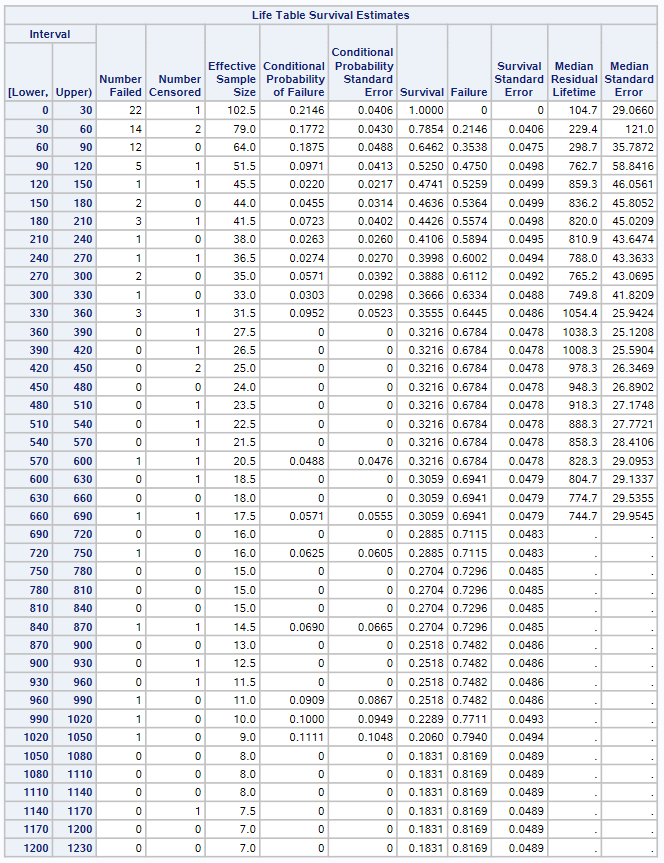
\includegraphics{sas/1a.PNG}

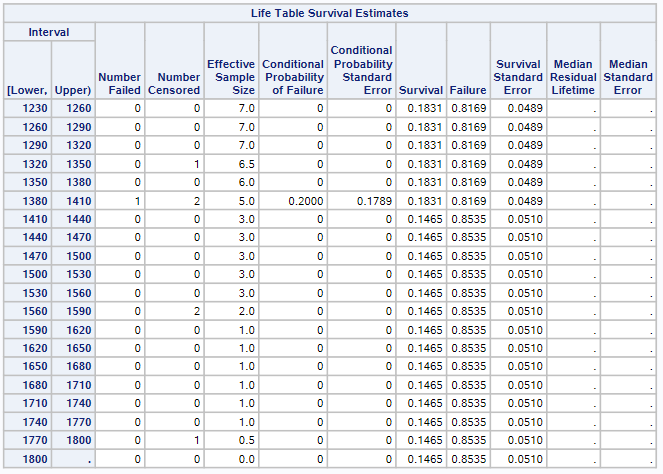
\includegraphics{sas/1b.PNG}

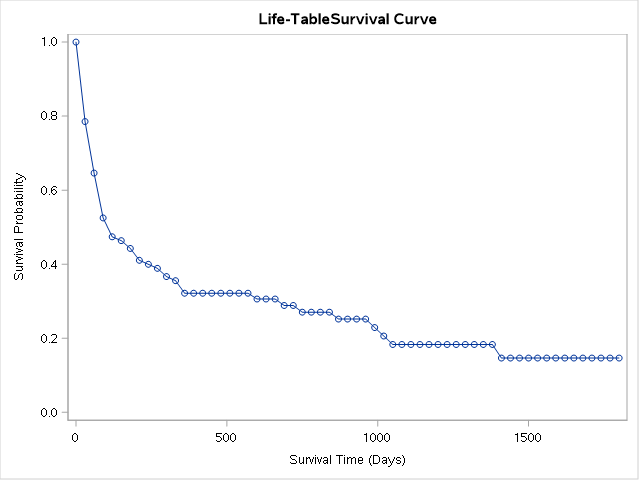
\includegraphics{sas/1c.png}

\hypertarget{muxe9thode-kaplan-meier-2}{%
\subsection{Méthode Kaplan-Meier}\label{muxe9thode-kaplan-meier-2}}

Le tableau des estimateurs ne sera pas reporté (voir intro du
document).\\
Pour récupérer ces estimateurs, on peut les récupérer via l'instruction
output et les exporter, par exemple, dans un tableur.

\begin{Shaded}
\begin{Highlighting}[]
\NormalTok{ods exclude Lifetest.Stratum1.ProductLimitEstimates;}
\NormalTok{proc lifetest data}\OtherTok{=}\NormalTok{trans;}
\NormalTok{time stime}\SpecialCharTok{*}\FunctionTok{died}\NormalTok{(}\DecValTok{0}\NormalTok{); run;}
\end{Highlighting}
\end{Shaded}

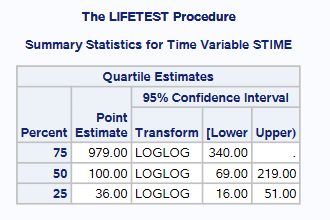
\includegraphics{sas/2a.PNG}

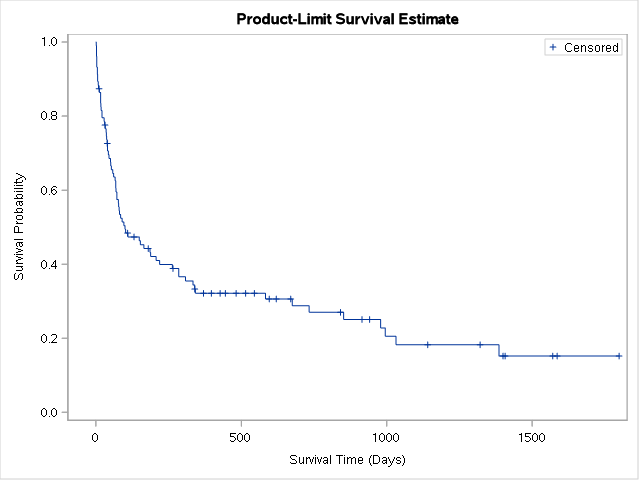
\includegraphics{sas/2b.png}

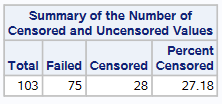
\includegraphics{sas/2c.PNG}

\textbf{Warning sur la durée moyenne reportée} Sauf exception ne pas
interpréter le tableau donnant la durée moyenne. Se reporter à
l'estimation des RMST plus bas.

\textbf{Comparaison des fonctions de survie}

\emph{Tests du log rank}

\begin{Shaded}
\begin{Highlighting}[]
\NormalTok{ods exclude Lifetest.Stratum1.ProductLimitEstimates Lifetest.Stratum2.ProductLimitEstimates ;}
\NormalTok{proc lifetest data}\OtherTok{=}\NormalTok{trans;}
\NormalTok{time stime}\SpecialCharTok{*}\FunctionTok{died}\NormalTok{(}\DecValTok{0}\NormalTok{);}
\NormalTok{strata surgery }\SpecialCharTok{/}\NormalTok{ test}\OtherTok{=}\NormalTok{all;}
\NormalTok{run;}
\end{Highlighting}
\end{Shaded}

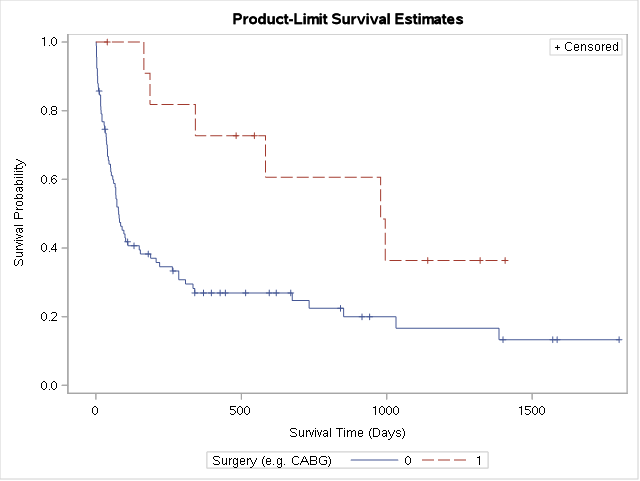
\includegraphics{sas/3a.png}

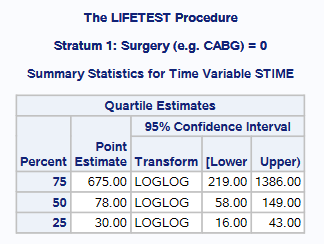
\includegraphics{sas/3b.PNG}

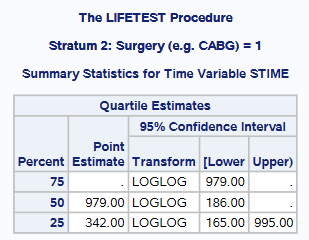
\includegraphics{sas/3c.PNG}

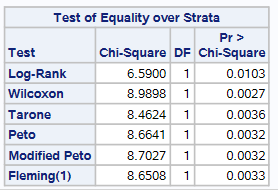
\includegraphics{sas/3d.PNG}

\emph{Comparaison des RMST}

Disponible avec le dernier module stat de Sas base (Sas-Stat 15.1
novembre 2018).

\begin{Shaded}
\begin{Highlighting}[]
\NormalTok{ods exclude Lifetest.Stratum1.ProductLimitEstimates;}
\NormalTok{proc lifetest data}\OtherTok{=}\NormalTok{trans rmst plots}\OtherTok{=}\NormalTok{(rmst);}
\NormalTok{time stime}\SpecialCharTok{*}\FunctionTok{died}\NormalTok{(}\DecValTok{0}\NormalTok{);}
\NormalTok{strata surgery; run;}
\end{Highlighting}
\end{Shaded}

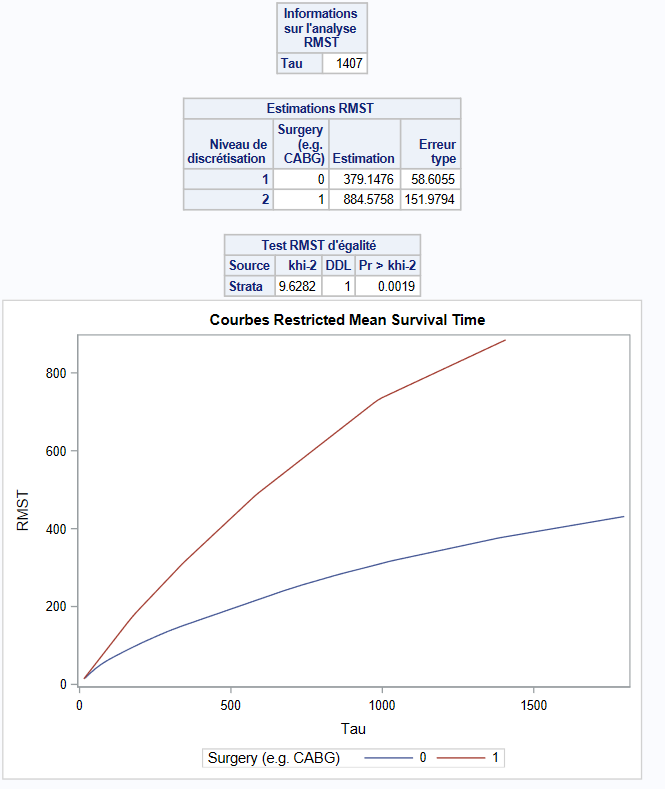
\includegraphics{sas/4.PNG}

\hypertarget{moduxe8le-de-cox-3}{%
\section{Modèle de Cox}\label{moduxe8le-de-cox-3}}

\hypertarget{estimation-du-moduxe8le-2}{%
\subsection{Estimation du modèle}\label{estimation-du-moduxe8le-2}}

\begin{Shaded}
\begin{Highlighting}[]
\NormalTok{proc phreg data}\OtherTok{=}\NormalTok{trans;}
\NormalTok{model stime}\SpecialCharTok{*}\FunctionTok{died}\NormalTok{(}\DecValTok{0}\NormalTok{) }\OtherTok{=}\NormalTok{ year age surgery ;}
\NormalTok{run;}
\end{Highlighting}
\end{Shaded}

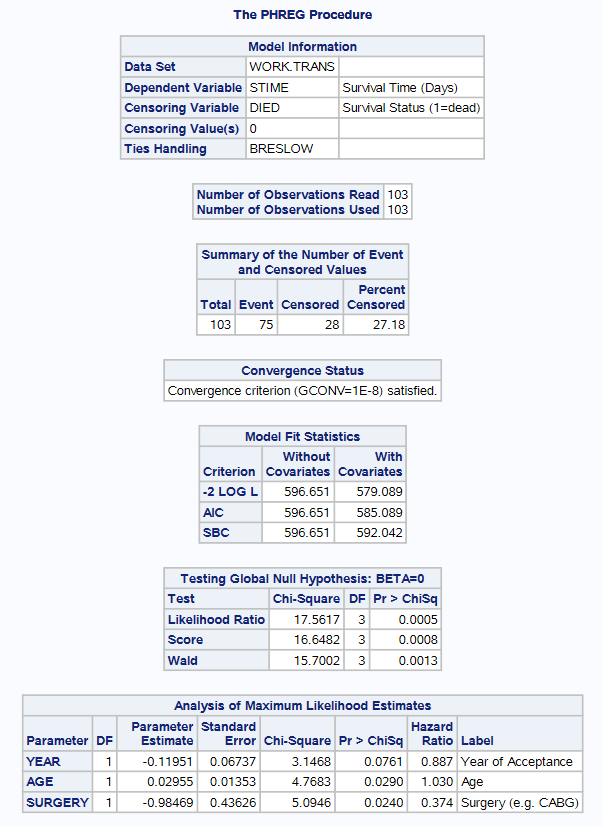
\includegraphics{sas/5a.PNG}

\hypertarget{tests-de-lhypothuxe8se-ph}{%
\subsection{Tests de l'hypothèse PH}\label{tests-de-lhypothuxe8se-ph}}

\hypertarget{test-de-grambsch-therneau}{%
\subsubsection{Test de Grambsch
Therneau}\label{test-de-grambsch-therneau}}

Demande au moins l'avant dernière version de Sas/Stat (2016?).

Le test est exécuté directement dans l'instruction \texttt{phreg}
(ajouter \texttt{zph}). L'option global permet de récupérer le résultat
du test omnibus (attention rejette facilement \(H_0\) - hypothèse PH
respectée - lorsque le nombre de degrés de liberté est élevé).

\begin{Shaded}
\begin{Highlighting}[]
\NormalTok{ods select PHReg.zphTest;}
\NormalTok{proc phreg data}\OtherTok{=}\NormalTok{trans }\FunctionTok{zph}\NormalTok{(global noplot);}
\NormalTok{model stime}\SpecialCharTok{*}\FunctionTok{died}\NormalTok{(}\DecValTok{0}\NormalTok{) }\OtherTok{=}\NormalTok{ year age surgery ;}
\NormalTok{run;}
\end{Highlighting}
\end{Shaded}

\includegraphics{sas/5b.PNG}

Par défaut SAS utilise la transformation \(f(t)=t\) (idem Stata). Pour
obtenir l'option par défaut de R \(f(t) = 1 - KM(t)\):

\begin{Shaded}
\begin{Highlighting}[]
\NormalTok{ods select PHReg.zphTest;}
\NormalTok{proc phreg data}\OtherTok{=}\NormalTok{trans }\FunctionTok{zph}\NormalTok{(global noplot }\AttributeTok{transform=}\NormalTok{km);}
\NormalTok{model stime}\SpecialCharTok{*}\FunctionTok{died}\NormalTok{(}\DecValTok{0}\NormalTok{) }\OtherTok{=}\NormalTok{ year age surgery ;}
\NormalTok{run;}
\end{Highlighting}
\end{Shaded}

\includegraphics{sas/5c.PNG}

\hypertarget{interaction-avec-la-duruxe9e}{%
\subsubsection{Interaction avec la
durée}\label{interaction-avec-la-duruxe9e}}

\textbf{Estimation d'un modèle avec indicatrices}\\
La covariable doit être sous forme d'indicatrice (binaire: (0,1)). Ce
qui est le cas ici avec la variable \emph{surgery}.

Exemple avec une covariable X à 3 modalités codée 1,2,3.

Estimation du modèle de Cox avec l'instruction \texttt{class} (ref: X=1)

\begin{Shaded}
\begin{Highlighting}[]
\NormalTok{proc phreg data}\OtherTok{=}\NormalTok{base;}
\NormalTok{class }\FunctionTok{X}\NormalTok{(}\AttributeTok{ref=}\StringTok{"1"}\NormalTok{);}
\NormalTok{model variable\_dur}\SpecialCharTok{*}\FunctionTok{variable\_cens}\NormalTok{(}\DecValTok{0}\NormalTok{) }\OtherTok{=}\NormalTok{ X; run;}
\end{Highlighting}
\end{Shaded}

Estimation du modèle de Cox avec indicatrices

\begin{Shaded}
\begin{Highlighting}[]
\NormalTok{data base; set base;}
\NormalTok{X1 }\OtherTok{=}\NormalTok{ X}\OtherTok{=}\DecValTok{1}\NormalTok{;}
\NormalTok{X2 }\OtherTok{=}\NormalTok{ X}\OtherTok{=}\DecValTok{2}\NormalTok{;}
\NormalTok{X3 }\OtherTok{=}\NormalTok{ X}\OtherTok{=}\DecValTok{3}\NormalTok{; run;}

\NormalTok{proc phreg data}\OtherTok{=}\NormalTok{base;}
\NormalTok{model variable\_dur}\SpecialCharTok{*}\FunctionTok{variable\_cens}\NormalTok{(}\DecValTok{0}\NormalTok{) }\OtherTok{=}\NormalTok{ X2 X3; run;}
\end{Highlighting}
\end{Shaded}

La variable d'intéraction (\(surgeryt = surgery\times stime\)) est
générée, le temps de l'estimation après l'instruction \texttt{model}.

\begin{Shaded}
\begin{Highlighting}[]
\NormalTok{ods select PHReg.ParameterEstimates;}
\NormalTok{proc phreg data}\OtherTok{=}\NormalTok{trans ;}
\NormalTok{model stime}\SpecialCharTok{*}\FunctionTok{died}\NormalTok{(}\DecValTok{0}\NormalTok{) }\OtherTok{=}\NormalTok{ year age surgery surgeryt ;}
\NormalTok{surgeryt }\OtherTok{=}\NormalTok{ surgery}\SpecialCharTok{*}\NormalTok{stime;}
\NormalTok{run;}
\end{Highlighting}
\end{Shaded}

\includegraphics{sas/5d.PNG}

\hypertarget{variable-dynamique}{%
\subsection{Variable dynamique}\label{variable-dynamique}}

\textbf{Warning: opération en `aveugle'}

Contrairement à R et Stata, la base n'a pas à être splittée, on ne peut
pas vérifier si la variable dynamique a été correctement créée. La
variable dynamique, qui peut être appréhendée comme une variable en
intéraction avec la durée, est générée après l'instruction
\texttt{model}.\\
Ici la tvc prendra la valeur 1 lorsque \emph{stime\textgreater wait}, 0
sinon.

\begin{Shaded}
\begin{Highlighting}[]
\NormalTok{ods select PHReg.ParameterEstimates;}
\NormalTok{proc phreg data}\OtherTok{=}\NormalTok{trans;}
\NormalTok{model stime}\SpecialCharTok{*}\FunctionTok{died}\NormalTok{(}\DecValTok{0}\NormalTok{) }\OtherTok{=}\NormalTok{ year age surgery tvc ;}
\NormalTok{tvc }\OtherTok{=}\NormalTok{ transplant}\OtherTok{=}\DecValTok{1}\NormalTok{ and stime}\SpecialCharTok{\textgreater{}=}\NormalTok{wait;}
\NormalTok{run;}
\end{Highlighting}
\end{Shaded}

\includegraphics{sas/6.PNG}

\hypertarget{moduxe8le-uxe0-temps-discret-2}{%
\section{Modèle à temps discret}\label{moduxe8le-uxe0-temps-discret-2}}

\hypertarget{mise-en-forme}{%
\subsection{Mise en forme}\label{mise-en-forme}}

On utilise une boucle pour répliquer les lignes sur la valeur de la
durée. La nouvelle variable de durée (t) sous forme de compteur est
générée automatiquement.

\begin{Shaded}
\begin{Highlighting}[]
\NormalTok{data td; set trans; }
\NormalTok{do t}\OtherTok{=}\DecValTok{1}\NormalTok{ to mois; }
\NormalTok{     output; }
\NormalTok{     end; run;}
     
\NormalTok{data td; set td;}
\ControlFlowTok{if}\NormalTok{ t}\SpecialCharTok{\textless{}}\NormalTok{mois then died}\OtherTok{=}\DecValTok{0}\NormalTok{;}
\NormalTok{t2}\OtherTok{=}\NormalTok{t}\SpecialCharTok{*}\NormalTok{t;}
\NormalTok{t3}\OtherTok{=}\NormalTok{t2}\SpecialCharTok{*}\NormalTok{t; run;}
\end{Highlighting}
\end{Shaded}

\hypertarget{duruxe9e-continue}{%
\subsection{Durée continue}\label{duruxe9e-continue}}

\emph{Estimation du modèle}

\begin{Shaded}
\begin{Highlighting}[]
\NormalTok{ods select Logistic.FitStatistics;}
\NormalTok{proc logistic data}\OtherTok{=}\NormalTok{td;}
\NormalTok{model }\FunctionTok{died}\NormalTok{(}\AttributeTok{ref=}\StringTok{"0"}\NormalTok{) }\OtherTok{=}\NormalTok{ t t2 t3 year age surgery  ; run;}
\end{Highlighting}
\end{Shaded}

\includegraphics{sas/7a.PNG}

\hypertarget{duruxe9e-discruxe8te}{%
\subsection{Durée discrète}\label{duruxe9e-discruxe8te}}

Pour l'exemple on va regrouper la durée par ses quartiles. Pour chaque
individu, on conserve seulement une observation dans chaque quartile.

\begin{Shaded}
\begin{Highlighting}[]
\NormalTok{proc rank data}\OtherTok{=}\NormalTok{td out}\OtherTok{=}\NormalTok{td2 groups}\OtherTok{=}\DecValTok{4}\NormalTok{;}
\NormalTok{var t;}
\NormalTok{ranks tq4;}
\NormalTok{run;}

\NormalTok{data td2; set td2;}
\NormalTok{id2}\OtherTok{=}\FunctionTok{put}\NormalTok{(id, }\FloatTok{3.}\NormalTok{);}
\NormalTok{tq42}\OtherTok{=}\FunctionTok{put}\NormalTok{(tq4, }\FloatTok{1.}\NormalTok{);}
\NormalTok{g}\OtherTok{=}\NormalTok{id2 }\SpecialCharTok{||}\NormalTok{ tq42; run;}

\NormalTok{proc sort data}\OtherTok{=}\NormalTok{td2; by id tq4; run;}

\NormalTok{data td2; set td2;}
\NormalTok{by g;}
\ControlFlowTok{if}\NormalTok{ LAST.g; run;}
\end{Highlighting}
\end{Shaded}

\emph{Estimation}

\begin{Shaded}
\begin{Highlighting}[]
\NormalTok{proc logistic data}\OtherTok{=}\NormalTok{td2;}
\NormalTok{class tq4 }\SpecialCharTok{/}\NormalTok{ param}\OtherTok{=}\NormalTok{ref;}
\NormalTok{model }\FunctionTok{died}\NormalTok{(}\AttributeTok{ref=}\StringTok{"0"}\NormalTok{) }\OtherTok{=}\NormalTok{ tq4 year age surgery; run;}
\end{Highlighting}
\end{Shaded}

\includegraphics{sas/7c.PNG}

\includegraphics{sas/7d.PNG}

\hypertarget{moduxe8les-paramuxe9trique}{%
\section{Modèles paramétrique}\label{moduxe8les-paramuxe9trique}}

On utilise la procédure proc \textbf{\texttt{lifereg}} et on indique le
type de distribution

\begin{Shaded}
\begin{Highlighting}[]
\NormalTok{proc lifereg data}\OtherTok{=}\NormalTok{trans;}
\NormalTok{model stime}\SpecialCharTok{*}\FunctionTok{died}\NormalTok{(}\DecValTok{0}\NormalTok{) }\OtherTok{=}\NormalTok{ year age surgery }\SpecialCharTok{/}\NormalTok{D}\OtherTok{=}\NormalTok{WEIBULL;}
\NormalTok{run;}
\end{Highlighting}
\end{Shaded}

\includegraphics{sas/8a.PNG}

\includegraphics{sas/8b.PNG}

\begin{Shaded}
\begin{Highlighting}[]
\NormalTok{proc lifereg data}\OtherTok{=}\NormalTok{trans;}
\NormalTok{model stime}\SpecialCharTok{*}\FunctionTok{died}\NormalTok{(}\DecValTok{0}\NormalTok{) }\OtherTok{=}\NormalTok{ year age surgery }\SpecialCharTok{/}\NormalTok{D}\OtherTok{=}\NormalTok{LLOGISTIC;}
\NormalTok{run;}
\end{Highlighting}
\end{Shaded}

\includegraphics{sas/8c.PNG}

\includegraphics{sas/8d.PNG}

\hypertarget{risques-concurrents-3}{%
\section{Risques concurrents}\label{risques-concurrents-3}}

\hypertarget{non-paramuxe9trique}{%
\subsection{Non paramétrique}\label{non-paramuxe9trique}}

On indique en option la cause d'intérêt avec
\textbf{\texttt{eventcode=valeur}} , les autres étant considérées commes
des risques concurrents.

\begin{Shaded}
\begin{Highlighting}[]
\NormalTok{proc lifetest data}\OtherTok{=}\NormalTok{trans plots}\OtherTok{=}\NormalTok{CIF;}
\NormalTok{time stime}\SpecialCharTok{*}\FunctionTok{compet}\NormalTok{(}\DecValTok{0}\NormalTok{) }\SpecialCharTok{/}\NormalTok{ eventcode}\OtherTok{=}\DecValTok{1}\NormalTok{; run;}
\end{Highlighting}
\end{Shaded}

\includegraphics{sas/9a.PNG}

\includegraphics{sas/9b.PNG}

\includegraphics{sas/9c.png}

Pour récupérer le test de Gray, on utilise l'instruction
\texttt{strata}.

\begin{Shaded}
\begin{Highlighting}[]
\NormalTok{proc lifetest data}\OtherTok{=}\NormalTok{trans plots}\OtherTok{=}\NormalTok{CIF;}
\NormalTok{time stime}\SpecialCharTok{*}\FunctionTok{compet}\NormalTok{(}\DecValTok{0}\NormalTok{) }\SpecialCharTok{/}\NormalTok{ eventcode}\OtherTok{=}\DecValTok{1}
\NormalTok{strata surgery; run;}
\end{Highlighting}
\end{Shaded}

\includegraphics{sas/9f.PNG}

\includegraphics{sas/9g.PNG}

\hypertarget{moduxe8le-logistique-multinomial-uxe0-duruxe9e-discruxe8te}{%
\subsection{Modèle logistique multinomial à durée
discrète}\label{moduxe8le-logistique-multinomial-uxe0-duruxe9e-discruxe8te}}

\begin{Shaded}
\begin{Highlighting}[]
\NormalTok{data td; set trans; }
\NormalTok{do t}\OtherTok{=}\DecValTok{1}\NormalTok{ to mois; }
\NormalTok{     output; }
\NormalTok{     end; }
\NormalTok{run;}
\NormalTok{data td; set td;}
\ControlFlowTok{if}\NormalTok{ t}\SpecialCharTok{\textless{}}\NormalTok{mois then compet}\OtherTok{=}\DecValTok{0}\NormalTok{;}
\NormalTok{t2}\OtherTok{=}\NormalTok{t}\SpecialCharTok{*}\NormalTok{t}
\NormalTok{run;}
\end{Highlighting}
\end{Shaded}

\begin{Shaded}
\begin{Highlighting}[]
\NormalTok{proc logistic data}\OtherTok{=}\NormalTok{td;}
\NormalTok{model }\FunctionTok{compet}\NormalTok{(}\AttributeTok{ref=}\StringTok{"0"}\NormalTok{) }\OtherTok{=}\NormalTok{ t t2 year age surgery }\SpecialCharTok{/}\NormalTok{ link}\OtherTok{=}\NormalTok{glogit;}
\NormalTok{run;}
\end{Highlighting}
\end{Shaded}

\includegraphics{sas/9i.PNG}

\includegraphics{sas/9j.PNG}

\hypertarget{python-6}{%
\chapter{\texorpdfstring{\textbf{Python}}{Python}}\label{python-6}}

\begin{tcolorbox}[enhanced jigsaw, arc=.35mm, bottomrule=.15mm, titlerule=0mm, colbacktitle=quarto-callout-note-color!10!white, left=2mm, opacitybacktitle=0.6, toprule=.15mm, title=\textcolor{quarto-callout-note-color}{\faInfo}\hspace{0.5em}{Note}, colframe=quarto-callout-note-color-frame, breakable, coltitle=black, opacityback=0, toptitle=1mm, bottomtitle=1mm, rightrule=.15mm, leftrule=.75mm, colback=white]

\begin{itemize}
\tightlist
\item
  Le document qui suit n'est qu'un programme fait il y a 3-4 ans.
  Utilisant très peu Python, je n'ai pas documenté les fonctions, plus
  ou moins obsures, qui ont été utilisées.
\item
  L'exécution a été réalisé le noyau \texttt{python3} de jupyter.
\item
  Le document n'a pas été compilé en PDF, seule cette version html est
  disponible.
\end{itemize}

\end{tcolorbox}

Deux paquets d'analyse: principalement \texttt{lifelines} (km, cox,
aft\ldots) et `statsmodels``` (estimation logit en temps discret,
kaplan-Meier, Cox).

Le package \texttt{statsmodels} est également ne mesure d'estimer des
courbes de séjour de type Kaplan-Meier et des modèles à risque
proportionnel de Cox. Le package \texttt{lifelines} couvre la quasi
totalité des méthodes standards, à l'exception des les risques
concurrents.

\begin{Shaded}
\begin{Highlighting}[]
\ImportTok{import}\NormalTok{ numpy  }\ImportTok{as}\NormalTok{ np}
\ImportTok{import}\NormalTok{ pandas }\ImportTok{as}\NormalTok{ pd}
\ImportTok{import}\NormalTok{ patsy  }\ImportTok{as}\NormalTok{ pt}
\ImportTok{import}\NormalTok{ lifelines }\ImportTok{as}\NormalTok{ lf}
\ImportTok{import}\NormalTok{ matplotlib.pyplot }\ImportTok{as}\NormalTok{ plt}
\ImportTok{import}\NormalTok{ statsmodels }\ImportTok{as}\NormalTok{ sm}
\end{Highlighting}
\end{Shaded}

Chargement de la base

\begin{Shaded}
\begin{Highlighting}[]
\NormalTok{trans }\OperatorTok{=}\NormalTok{ pd.read\_csv(}\StringTok{"https://raw.githubusercontent.com/mthevenin/analyse\_duree/master/bases/transplantation.csv"}\NormalTok{)}

\NormalTok{trans.head(}\DecValTok{10}\NormalTok{)}
\NormalTok{trans.info()}
\end{Highlighting}
\end{Shaded}

\begin{verbatim}
<class 'pandas.core.frame.DataFrame'>
RangeIndex: 103 entries, 0 to 102
Data columns (total 10 columns):
 #   Column      Non-Null Count  Dtype
---  ------      --------------  -----
 0   id          103 non-null    int64
 1   year        103 non-null    int64
 2   age         103 non-null    int64
 3   died        103 non-null    int64
 4   stime       103 non-null    int64
 5   surgery     103 non-null    int64
 6   transplant  103 non-null    int64
 7   wait        103 non-null    int64
 8   mois        103 non-null    int64
 9   compet      103 non-null    int64
dtypes: int64(10)
memory usage: 8.2 KB
\end{verbatim}

\hypertarget{package-lifelines}{%
\section{Package lifelines}\label{package-lifelines}}

\textbf{Documentation}:
\url{https://lifelines.readthedocs.io/en/latest/}

\hypertarget{non-paramuxe9trique-kaplan-meier}{%
\subsection{Non Paramétrique: Kaplan
Meier}\label{non-paramuxe9trique-kaplan-meier}}

\textbf{Estimateur KM et durée médiane}

\begin{Shaded}
\begin{Highlighting}[]
\NormalTok{T }\OperatorTok{=}\NormalTok{ trans[}\StringTok{\textquotesingle{}stime\textquotesingle{}}\NormalTok{]}
\NormalTok{E }\OperatorTok{=}\NormalTok{ trans[}\StringTok{\textquotesingle{}died\textquotesingle{}}\NormalTok{]}


\ImportTok{from}\NormalTok{ lifelines }\ImportTok{import}\NormalTok{ KaplanMeierFitter}
\NormalTok{kmf }\OperatorTok{=}\NormalTok{ KaplanMeierFitter()}
\NormalTok{kmf.fit(T,E)}
\BuiltInTok{print}\NormalTok{(kmf.survival\_function\_)}
\NormalTok{a }\OperatorTok{=} \StringTok{"DUREE MEDIANE:"}
\NormalTok{b }\OperatorTok{=}\NormalTok{ kmf.median\_survival\_time\_}
\BuiltInTok{print}\NormalTok{(a,b)}
\end{Highlighting}
\end{Shaded}

\begin{verbatim}
          KM_estimate
timeline             
0.0          1.000000
1.0          0.990291
2.0          0.961165
3.0          0.932039
5.0          0.912621
...               ...
1400.0       0.151912
1407.0       0.151912
1571.0       0.151912
1586.0       0.151912
1799.0       0.151912

[89 rows x 1 columns]
DUREE MEDIANE: 100.0
\end{verbatim}

\begin{Shaded}
\begin{Highlighting}[]
\NormalTok{kmf.plot()}
\end{Highlighting}
\end{Shaded}

\begin{verbatim}
<AxesSubplot: xlabel='timeline'>
\end{verbatim}

\begin{figure}[H]

{\centering \includegraphics{17-Python_files/figure-pdf/cell-5-output-2.pdf}

}

\end{figure}

\textbf{Comparaison des fonctions de survie}

\begin{Shaded}
\begin{Highlighting}[]
\NormalTok{ax }\OperatorTok{=}\NormalTok{ plt.subplot(}\DecValTok{111}\NormalTok{)}
\NormalTok{kmf }\OperatorTok{=}\NormalTok{ KaplanMeierFitter()}
\ControlFlowTok{for}\NormalTok{ name, grouped\_df }\KeywordTok{in}\NormalTok{ trans.groupby(}\StringTok{\textquotesingle{}surgery\textquotesingle{}}\NormalTok{):}
\NormalTok{    kmf.fit(grouped\_df[}\StringTok{\textquotesingle{}stime\textquotesingle{}}\NormalTok{], grouped\_df[}\StringTok{\textquotesingle{}died\textquotesingle{}}\NormalTok{], label}\OperatorTok{=}\NormalTok{name)}
\NormalTok{    kmf.plot(ax}\OperatorTok{=}\NormalTok{ax)}
\end{Highlighting}
\end{Shaded}

\begin{figure}[H]

{\centering \includegraphics{17-Python_files/figure-pdf/cell-6-output-1.pdf}

}

\end{figure}

\begin{Shaded}
\begin{Highlighting}[]
\ImportTok{from}\NormalTok{ lifelines.statistics }\ImportTok{import}\NormalTok{ multivariate\_logrank\_test}
\NormalTok{results }\OperatorTok{=}\NormalTok{ multivariate\_logrank\_test(trans[}\StringTok{\textquotesingle{}stime\textquotesingle{}}\NormalTok{], trans[}\StringTok{\textquotesingle{}surgery\textquotesingle{}}\NormalTok{], trans[}\StringTok{\textquotesingle{}died\textquotesingle{}}\NormalTok{])}
\NormalTok{results.print\_summary()}
\end{Highlighting}
\end{Shaded}

\begin{tabular}{lrrr}
 & test_statistic & p & -log2(p) \\
0 & 6.59 & 0.01 & 6.61 \\
\end{tabular}

\hypertarget{semi-paramuxe9trique-cox}{%
\section{Semi paramétrique: Cox}\label{semi-paramuxe9trique-cox}}

\hypertarget{estimation-2}{%
\subsection{Estimation}\label{estimation-2}}

\begin{Shaded}
\begin{Highlighting}[]
\NormalTok{model }\OperatorTok{=} \StringTok{\textquotesingle{}year + age + C(surgery) {-}1\textquotesingle{}}
\NormalTok{X }\OperatorTok{=}\NormalTok{ pt.dmatrix(model, trans, return\_type}\OperatorTok{=}\StringTok{\textquotesingle{}dataframe\textquotesingle{}}\NormalTok{)}
\NormalTok{design\_info }\OperatorTok{=}\NormalTok{ X.design\_info}
\NormalTok{YX }\OperatorTok{=}\NormalTok{ X.join(trans[[}\StringTok{\textquotesingle{}stime\textquotesingle{}}\NormalTok{,}\StringTok{\textquotesingle{}died\textquotesingle{}}\NormalTok{]])}
\NormalTok{YX.drop([}\StringTok{\textquotesingle{}C(surgery)[0]\textquotesingle{}}\NormalTok{], axis}\OperatorTok{=}\DecValTok{1}\NormalTok{, inplace}\OperatorTok{=}\VariableTok{True}\NormalTok{)}
\NormalTok{YX.head()}


\ImportTok{from}\NormalTok{ lifelines }\ImportTok{import}\NormalTok{ CoxPHFitter}
\NormalTok{cph }\OperatorTok{=}\NormalTok{ CoxPHFitter()}
\NormalTok{cph.fit(YX, duration\_col}\OperatorTok{=}\StringTok{\textquotesingle{}stime\textquotesingle{}}\NormalTok{, event\_col}\OperatorTok{=}\StringTok{\textquotesingle{}died\textquotesingle{}}\NormalTok{)}
\NormalTok{cph.print\_summary()}
\NormalTok{cph.plot()}
\end{Highlighting}
\end{Shaded}

\begin{tabular}{lrrrrrrrrrrr}
 & coef & exp(coef) & se(coef) & coef lower 95% & coef upper 95% & exp(coef) lower 95% & exp(coef) upper 95% & cmp to & z & p & -log2(p) \\
covariate &  &  &  &  &  &  &  &  &  &  &  \\
C(surgery)[1] & -0.99 & 0.37 & 0.44 & -1.84 & -0.13 & 0.16 & 0.88 & 0.00 & -2.26 & 0.02 & 5.40 \\
year & -0.12 & 0.89 & 0.07 & -0.25 & 0.01 & 0.78 & 1.01 & 0.00 & -1.78 & 0.08 & 3.72 \\
age & 0.03 & 1.03 & 0.01 & 0.00 & 0.06 & 1.00 & 1.06 & 0.00 & 2.19 & 0.03 & 5.12 \\
\end{tabular}

\begin{verbatim}
<AxesSubplot: xlabel='log(HR) (95% CI)'>
\end{verbatim}

\begin{figure}[H]

{\centering \includegraphics{17-Python_files/figure-pdf/cell-8-output-3.pdf}

}

\end{figure}

\hypertarget{tests-hypothuxe8se-ph}{%
\subsection{Tests hypothèse PH}\label{tests-hypothuxe8se-ph}}

\textbf{Test PH: Schoenfeld Méthode 1}

\begin{Shaded}
\begin{Highlighting}[]
\NormalTok{cph.check\_assumptions(YX,p\_value\_threshold}\OperatorTok{=}\FloatTok{0.05}\NormalTok{)}
\end{Highlighting}
\end{Shaded}

\begin{verbatim}
The ``p_value_threshold`` is set at 0.05. Even under the null hypothesis of no violations, some
covariates will be below the threshold by chance. This is compounded when there are many covariates.
Similarly, when there are lots of observations, even minor deviances from the proportional hazard
assumption will be flagged.

With that in mind, it's best to use a combination of statistical tests and visual tests to determine
the most serious violations. Produce visual plots using ``check_assumptions(..., show_plots=True)``
and looking for non-constant lines. See link [A] below for a full example.
\end{verbatim}

\begin{tabular}{llrrr}
 &  & test_statistic & p & -log2(p) \\
\multirow[c]{2}{*}{C(surgery)[1]} & km & 4.01 & 0.05 & 4.47 \\
 & rank & 3.74 & 0.05 & 4.23 \\
\multirow[c]{2}{*}{age} & km & 1.18 & 0.28 & 1.86 \\
 & rank & 1.06 & 0.30 & 1.72 \\
\multirow[c]{2}{*}{year} & km & 2.07 & 0.15 & 2.73 \\
 & rank & 2.08 & 0.15 & 2.75 \\
\end{tabular}

\begin{verbatim}


1. Variable 'C(surgery)[1]' failed the non-proportional test: p-value is 0.0452.

   Advice: with so few unique values (only 2), you can include `strata=['C(surgery)[1]', ...]` in
the call in `.fit`. See documentation in link [E] below.

---
[A]  https://lifelines.readthedocs.io/en/latest/jupyter_notebooks/Proportional%20hazard%20assumption.html
[B]  https://lifelines.readthedocs.io/en/latest/jupyter_notebooks/Proportional%20hazard%20assumption.html#Bin-variable-and-stratify-on-it
[C]  https://lifelines.readthedocs.io/en/latest/jupyter_notebooks/Proportional%20hazard%20assumption.html#Introduce-time-varying-covariates
[D]  https://lifelines.readthedocs.io/en/latest/jupyter_notebooks/Proportional%20hazard%20assumption.html#Modify-the-functional-form
[E]  https://lifelines.readthedocs.io/en/latest/jupyter_notebooks/Proportional%20hazard%20assumption.html#Stratification
\end{verbatim}

\begin{verbatim}
[]
\end{verbatim}

\textbf{Test PH: Schoenfeld Méthode 2}

\begin{Shaded}
\begin{Highlighting}[]
\ImportTok{from}\NormalTok{ lifelines.statistics }\ImportTok{import}\NormalTok{  proportional\_hazard\_test }
\NormalTok{zph }\OperatorTok{=}\NormalTok{ proportional\_hazard\_test(cph, YX, time\_transform}\OperatorTok{=}\StringTok{\textquotesingle{}all\textquotesingle{}}\NormalTok{)}
\NormalTok{zph.print\_summary()}
\end{Highlighting}
\end{Shaded}

\begin{tabular}{llrrr}
 &  & test_statistic & p & -log2(p) \\
\multirow[c]{4}{*}{C(surgery)[1]} & identity & 5.54 & 0.02 & 5.75 \\
 & km & 4.01 & 0.05 & 4.47 \\
 & log & 3.69 & 0.05 & 4.19 \\
 & rank & 3.74 & 0.05 & 4.23 \\
\multirow[c]{4}{*}{age} & identity & 1.61 & 0.20 & 2.29 \\
 & km & 1.18 & 0.28 & 1.86 \\
 & log & 0.61 & 0.44 & 1.20 \\
 & rank & 1.06 & 0.30 & 1.72 \\
\multirow[c]{4}{*}{year} & identity & 0.80 & 0.37 & 1.43 \\
 & km & 2.07 & 0.15 & 2.73 \\
 & log & 1.34 & 0.25 & 2.02 \\
 & rank & 2.08 & 0.15 & 2.75 \\
\end{tabular}

\textbf{Test PH: intéraction}

\begin{Shaded}
\begin{Highlighting}[]
\ImportTok{from}\NormalTok{ lifelines.utils }\ImportTok{import}\NormalTok{ to\_episodic\_format}
\ImportTok{from}\NormalTok{ lifelines }\ImportTok{import}\NormalTok{ CoxTimeVaryingFitter}
\end{Highlighting}
\end{Shaded}

\emph{Transformation de la base YX}

\begin{Shaded}
\begin{Highlighting}[]
\BuiltInTok{long} \OperatorTok{=}\NormalTok{ to\_episodic\_format(YX, duration\_col}\OperatorTok{=}\StringTok{\textquotesingle{}stime\textquotesingle{}}\NormalTok{, event\_col}\OperatorTok{=}\StringTok{\textquotesingle{}died\textquotesingle{}}\NormalTok{)}
\end{Highlighting}
\end{Shaded}

\emph{Création de la variable d'intéraction}

\begin{Shaded}
\begin{Highlighting}[]
\BuiltInTok{long}\NormalTok{[}\StringTok{\textquotesingle{}surgery\_t\textquotesingle{}}\NormalTok{] }\OperatorTok{=} \BuiltInTok{long}\NormalTok{[}\StringTok{\textquotesingle{}C(surgery)[1]\textquotesingle{}}\NormalTok{] }\OperatorTok{*} \BuiltInTok{long}\NormalTok{[}\StringTok{\textquotesingle{}stop\textquotesingle{}}\NormalTok{]}
\end{Highlighting}
\end{Shaded}

\emph{Estimation}

\begin{Shaded}
\begin{Highlighting}[]
\NormalTok{ctv }\OperatorTok{=}\NormalTok{ CoxTimeVaryingFitter()}
\NormalTok{ctv.fit(}\BuiltInTok{long}\NormalTok{,}
\NormalTok{        id\_col}\OperatorTok{=}\StringTok{\textquotesingle{}id\textquotesingle{}}\NormalTok{,}
\NormalTok{        event\_col}\OperatorTok{=}\StringTok{\textquotesingle{}died\textquotesingle{}}\NormalTok{,}
\NormalTok{        start\_col}\OperatorTok{=}\StringTok{\textquotesingle{}start\textquotesingle{}}\NormalTok{,}
\NormalTok{        stop\_col}\OperatorTok{=}\StringTok{\textquotesingle{}stop\textquotesingle{}}\NormalTok{,)}
\NormalTok{ctv.print\_summary(}\DecValTok{4}\NormalTok{)}
\end{Highlighting}
\end{Shaded}

\begin{tabular}{lrrrrrrrrrrr}
 & coef & exp(coef) & se(coef) & coef lower 95% & coef upper 95% & exp(coef) lower 95% & exp(coef) upper 95% & cmp to & z & p & -log2(p) \\
covariate &  &  &  &  &  &  &  &  &  &  &  \\
C(surgery)[1] & -1.7547 & 0.1730 & 0.6743 & -3.0764 & -0.4331 & 0.0461 & 0.6485 & 0.0000 & -2.6022 & 0.0093 & 6.7542 \\
age & 0.0289 & 1.0293 & 0.0134 & 0.0025 & 0.0552 & 1.0025 & 1.0568 & 0.0000 & 2.1479 & 0.0317 & 4.9785 \\
year & -0.1231 & 0.8842 & 0.0668 & -0.2541 & 0.0079 & 0.7756 & 1.0080 & 0.0000 & -1.8415 & 0.0656 & 3.9312 \\
surgery_t & 0.0022 & 1.0022 & 0.0011 & 0.0001 & 0.0044 & 1.0001 & 1.0044 & 0.0000 & 2.0239 & 0.0430 & 4.5402 \\
\end{tabular}

\hypertarget{variable-dynamique-binaire}{%
\subsection{Variable dynamique
binaire}\label{variable-dynamique-binaire}}

\hypertarget{moduxe8le-uxe0-temps-discret-3}{%
\section{Modèle à temps discret}\label{moduxe8le-uxe0-temps-discret-3}}

\hypertarget{ajustement-continu}{%
\subsection{Ajustement continu}\label{ajustement-continu}}

Modèle logistique estimé avec le paquet \texttt{statsmodel}. La fonction
\texttt{to\_episodic\_format} de \texttt{lifelines} permet de mettre en
forme la base.\\
Pour la durée, on utilisera ici la variable \textbf{mois} (regroupement
de stime par intervalle de 30 jours).

\begin{Shaded}
\begin{Highlighting}[]
\ImportTok{import}\NormalTok{ statsmodels.formula.api }\ImportTok{as}\NormalTok{ smf }\CommentTok{\#type R formule =\textgreater{} ce qu\textquotesingle{}on utilisera\#}
\ImportTok{import}\NormalTok{ statsmodels.api }\ImportTok{as}\NormalTok{ sm }\CommentTok{\#type python\#}
\end{Highlighting}
\end{Shaded}

\textbf{Transformation de la base en format long}

\begin{Shaded}
\begin{Highlighting}[]
\NormalTok{td }\OperatorTok{=}\NormalTok{ pd.read\_csv(}\StringTok{"https://raw.githubusercontent.com/mthevenin/analyse\_duree/master/bases/transplantation.csv"}\NormalTok{)}
\NormalTok{td.drop([}\StringTok{\textquotesingle{}id\textquotesingle{}}\NormalTok{], axis}\OperatorTok{=}\DecValTok{1}\NormalTok{, inplace}\OperatorTok{=}\VariableTok{True}\NormalTok{)}
\NormalTok{td[}\StringTok{\textquotesingle{}dur\textquotesingle{}}\NormalTok{] }\OperatorTok{=}\NormalTok{ td[}\StringTok{\textquotesingle{}mois\textquotesingle{}}\NormalTok{]}
\NormalTok{td }\OperatorTok{=}\NormalTok{ to\_episodic\_format(td, duration\_col}\OperatorTok{=}\StringTok{\textquotesingle{}mois\textquotesingle{}}\NormalTok{, event\_col}\OperatorTok{=}\StringTok{\textquotesingle{}died\textquotesingle{}}\NormalTok{)}
\end{Highlighting}
\end{Shaded}

\textbf{Evaluation de l'ajustement avec des fonctions quadratiques}

\begin{Shaded}
\begin{Highlighting}[]
\NormalTok{td[}\StringTok{\textquotesingle{}t2\textquotesingle{}}\NormalTok{] }\OperatorTok{=}\NormalTok{ td[}\StringTok{\textquotesingle{}stop\textquotesingle{}}\NormalTok{]}\OperatorTok{**}\DecValTok{2}
\NormalTok{td[}\StringTok{\textquotesingle{}t3\textquotesingle{}}\NormalTok{] }\OperatorTok{=}\NormalTok{ td[}\StringTok{\textquotesingle{}stop\textquotesingle{}}\NormalTok{]}\OperatorTok{**}\DecValTok{3}
\NormalTok{fit1 }\OperatorTok{=}\NormalTok{ smf.glm(formula}\OperatorTok{=}  \StringTok{"died \textasciitilde{} stop"}\NormalTok{, data}\OperatorTok{=}\NormalTok{td, family}\OperatorTok{=}\NormalTok{sm.families.Binomial()).fit()}
\NormalTok{fit2 }\OperatorTok{=}\NormalTok{ smf.glm(formula}\OperatorTok{=}  \StringTok{"died \textasciitilde{} stop + t2"}\NormalTok{, data}\OperatorTok{=}\NormalTok{td, family}\OperatorTok{=}\NormalTok{sm.families.Binomial()).fit()}
\NormalTok{fit3 }\OperatorTok{=}\NormalTok{ smf.glm(formula}\OperatorTok{=}  \StringTok{"died \textasciitilde{} stop + t2 + t3"}\NormalTok{, data}\OperatorTok{=}\NormalTok{td, family}\OperatorTok{=}\NormalTok{sm.families.Binomial()).fit()}
\end{Highlighting}
\end{Shaded}

\textbf{Comparaison des AIC}

\begin{Shaded}
\begin{Highlighting}[]
\BuiltInTok{print}\NormalTok{(}\StringTok{"AIC pour ajustement t1"}\NormalTok{)}
\BuiltInTok{print}\NormalTok{(fit1.aic)}
\BuiltInTok{print}\NormalTok{(}\StringTok{"AIC pour ajustement durée t1 + t2"}\NormalTok{)}
\BuiltInTok{print}\NormalTok{(fit2.aic)}
\BuiltInTok{print}\NormalTok{(}\StringTok{"AIC pour ajustement durée t1 + t2 + t3"}\NormalTok{)}
\BuiltInTok{print}\NormalTok{(fit3.aic)}
\end{Highlighting}
\end{Shaded}

\begin{verbatim}
AIC pour ajustement t1
504.5211512753311
AIC pour ajustement durée t1 + t2
492.11522432726747
AIC pour ajustement durée t1 + t2 + t3
486.50534103180416
\end{verbatim}

\textbf{Estimation du modèle}

\begin{Shaded}
\begin{Highlighting}[]
\NormalTok{tdfit }\OperatorTok{=}\NormalTok{ smf.glm(formula}\OperatorTok{=}  \StringTok{"died \textasciitilde{} stop + t2 + t3 + year + age + surgery"}\NormalTok{, data}\OperatorTok{=}\NormalTok{td, family}\OperatorTok{=}\NormalTok{sm.families.Binomial()).fit()}
\NormalTok{tdfit.summary()}
\end{Highlighting}
\end{Shaded}

\begin{longtable}[]{@{}llll@{}}
\caption{Generalized Linear Model Regression Results}\tabularnewline
\toprule\noalign{}
\endfirsthead
\endhead
\bottomrule\noalign{}
\endlastfoot
Dep. Variable: & died & No. Observations: & 1127 \\
Model: & GLM & Df Residuals: & 1120 \\
Model Family: & Binomial & Df Model: & 6 \\
Link Function: & Logit & Scale: & 1.0000 \\
Method: & IRLS & Log-Likelihood: & -230.34 \\
Date: & Mon, 21 Aug 2023 & Deviance: & 460.67 \\
Time: & 13:47:11 & Pearson chi2: & 1.30e+03 \\
No. Iterations: & 7 & Pseudo R-squ. (CS): & 0.07732 \\
Covariance Type: & nonrobust & & \\
\end{longtable}

\begin{longtable}[]{@{}lllllll@{}}
\toprule\noalign{}
\endhead
\bottomrule\noalign{}
\endlastfoot
& coef & std err & z & P\textgreater\textbar z\textbar{} & {[}0.025 &
0.975{]} \\
Intercept & 7.0827 & 5.308 & 1.334 & 0.182 & -3.320 & 17.486 \\
stop & -0.3721 & 0.082 & -4.516 & 0.000 & -0.534 & -0.211 \\
t2 & 0.0142 & 0.005 & 2.835 & 0.005 & 0.004 & 0.024 \\
t3 & -0.0002 & 7.85e-05 & -2.113 & 0.035 & -0.000 & -1.2e-05 \\
year & -0.1327 & 0.074 & -1.798 & 0.072 & -0.277 & 0.012 \\
age & 0.0333 & 0.015 & 2.270 & 0.023 & 0.005 & 0.062 \\
surgery & -1.0109 & 0.449 & -2.254 & 0.024 & -1.890 & -0.132 \\
\end{longtable}

\hypertarget{ajustement-discret-1}{%
\subsection{Ajustement discret}\label{ajustement-discret-1}}

\emph{Création des intervalles pour l'exemple (quantile de la durée en
mois)}

\begin{Shaded}
\begin{Highlighting}[]
\NormalTok{td[}\StringTok{\textquotesingle{}ct4\textquotesingle{}}\NormalTok{] }\OperatorTok{=}\NormalTok{ pd.qcut(td[}\StringTok{\textquotesingle{}stop\textquotesingle{}}\NormalTok{],[}\DecValTok{0}\NormalTok{, }\FloatTok{.25}\NormalTok{, }\FloatTok{.5}\NormalTok{, }\FloatTok{.75}\NormalTok{, }\FloatTok{1.}\NormalTok{]) }
\NormalTok{td[}\StringTok{\textquotesingle{}ct4\textquotesingle{}}\NormalTok{].value\_counts(normalize}\OperatorTok{=}\VariableTok{True}\NormalTok{)}\OperatorTok{*}\DecValTok{100}
\NormalTok{td.ct4 }\OperatorTok{=}\NormalTok{ pd.Categorical(td.ct4)}
\NormalTok{td[}\StringTok{\textquotesingle{}ct4\textquotesingle{}}\NormalTok{] }\OperatorTok{=}\NormalTok{ td.ct4.cat.codes}
\end{Highlighting}
\end{Shaded}

Pour chaque individu, on conserve une seule observation par intervalle.

\begin{Shaded}
\begin{Highlighting}[]
\NormalTok{td2 }\OperatorTok{=}\NormalTok{ td }
\NormalTok{td2[}\StringTok{\textquotesingle{}t\textquotesingle{}}\NormalTok{] }\OperatorTok{=}\NormalTok{ td2[}\StringTok{\textquotesingle{}ct4\textquotesingle{}}\NormalTok{]}
\NormalTok{td2 }\OperatorTok{=}\NormalTok{ td2.sort\_values([}\StringTok{\textquotesingle{}id\textquotesingle{}}\NormalTok{, }\StringTok{\textquotesingle{}stop\textquotesingle{}}\NormalTok{])}
\NormalTok{td2 }\OperatorTok{=}\NormalTok{  td2.groupby([}\StringTok{\textquotesingle{}id\textquotesingle{}}\NormalTok{,}\StringTok{\textquotesingle{}ct4\textquotesingle{}}\NormalTok{]).last()}
\end{Highlighting}
\end{Shaded}

\textbf{Estimation}

\begin{Shaded}
\begin{Highlighting}[]
\NormalTok{td2fit }\OperatorTok{=}\NormalTok{ smf.glm(formula}\OperatorTok{=}  \StringTok{"died \textasciitilde{} C(t) +  year + age + surgery"}\NormalTok{, data}\OperatorTok{=}\NormalTok{td2, family}\OperatorTok{=}\NormalTok{sm.families.Binomial()).fit()}
\NormalTok{td2fit.summary()}
\end{Highlighting}
\end{Shaded}

\begin{longtable}[]{@{}llll@{}}
\caption{Generalized Linear Model Regression Results}\tabularnewline
\toprule\noalign{}
\endfirsthead
\endhead
\bottomrule\noalign{}
\endlastfoot
Dep. Variable: & died & No. Observations: & 197 \\
Model: & GLM & Df Residuals: & 190 \\
Model Family: & Binomial & Df Model: & 6 \\
Link Function: & Logit & Scale: & 1.0000 \\
Method: & IRLS & Log-Likelihood: & -111.24 \\
Date: & Mon, 21 Aug 2023 & Deviance: & 222.48 \\
Time: & 13:47:12 & Pearson chi2: & 221. \\
No. Iterations: & 4 & Pseudo R-squ. (CS): & 0.1808 \\
Covariance Type: & nonrobust & & \\
\end{longtable}

\begin{longtable}[]{@{}lllllll@{}}
\toprule\noalign{}
\endhead
\bottomrule\noalign{}
\endlastfoot
& coef & std err & z & P\textgreater\textbar z\textbar{} & {[}0.025 &
0.975{]} \\
Intercept & 12.4467 & 6.654 & 1.871 & 0.061 & -0.594 & 25.488 \\
C(t){[}T.1{]} & -1.0334 & 0.419 & -2.467 & 0.014 & -1.854 & -0.212 \\
C(t){[}T.2{]} & -1.6152 & 0.545 & -2.965 & 0.003 & -2.683 & -0.547 \\
C(t){[}T.3{]} & -0.4789 & 0.599 & -0.799 & 0.424 & -1.654 & 0.696 \\
year & -0.2032 & 0.093 & -2.181 & 0.029 & -0.386 & -0.021 \\
age & 0.0469 & 0.018 & 2.533 & 0.011 & 0.011 & 0.083 \\
surgery & -1.1102 & 0.503 & -2.209 & 0.027 & -2.095 & -0.125 \\
\end{longtable}

\hypertarget{moduxe8le-paramuxe9trique-de-type-aft}{%
\section{Modèle paramétrique de type
AFT}\label{moduxe8le-paramuxe9trique-de-type-aft}}

\begin{Shaded}
\begin{Highlighting}[]
\ImportTok{from}\NormalTok{ lifelines }\ImportTok{import}\NormalTok{ WeibullAFTFitter, LogLogisticAFTFitter}
\end{Highlighting}
\end{Shaded}

\textbf{Weibull}

\begin{Shaded}
\begin{Highlighting}[]
\NormalTok{aftw }\OperatorTok{=}\NormalTok{ WeibullAFTFitter()}
\NormalTok{aftw.fit(YX, duration\_col}\OperatorTok{=}\StringTok{\textquotesingle{}stime\textquotesingle{}}\NormalTok{, event\_col}\OperatorTok{=}\StringTok{\textquotesingle{}died\textquotesingle{}}\NormalTok{)}
\NormalTok{aftw.print\_summary()}
\end{Highlighting}
\end{Shaded}

\begin{tabular}{llrrrrrrrrrrr}
 &  & coef & exp(coef) & se(coef) & coef lower 95% & coef upper 95% & exp(coef) lower 95% & exp(coef) upper 95% & cmp to & z & p & -log2(p) \\
param & covariate &  &  &  &  &  &  &  &  &  &  &  \\
\multirow[c]{4}{*}{lambda_} & C(surgery)[1] & 1.97 & 7.17 & 0.78 & 0.44 & 3.50 & 1.56 & 33.05 & 0.00 & 2.53 & 0.01 & 6.45 \\
 & age & -0.06 & 0.94 & 0.02 & -0.11 & -0.01 & 0.90 & 0.99 & 0.00 & -2.49 & 0.01 & 6.28 \\
 & year & 0.16 & 1.18 & 0.12 & -0.08 & 0.40 & 0.93 & 1.49 & 0.00 & 1.33 & 0.18 & 2.44 \\
 & Intercept & -3.02 & 0.05 & 8.73 & -20.13 & 14.09 & 0.00 & 1310196.43 & 0.00 & -0.35 & 0.73 & 0.46 \\
rho_ & Intercept & -0.59 & 0.56 & 0.09 & -0.77 & -0.41 & 0.46 & 0.67 & 0.00 & -6.33 & 0.00 & 31.93 \\
\end{tabular}

\textbf{Loglogistique}

\begin{Shaded}
\begin{Highlighting}[]
\NormalTok{aftl }\OperatorTok{=}\NormalTok{ LogLogisticAFTFitter()}
\NormalTok{aftl.fit(YX, duration\_col}\OperatorTok{=}\StringTok{\textquotesingle{}stime\textquotesingle{}}\NormalTok{, event\_col}\OperatorTok{=}\StringTok{\textquotesingle{}died\textquotesingle{}}\NormalTok{)}
\NormalTok{aftl.print\_summary()}
\end{Highlighting}
\end{Shaded}

\begin{tabular}{llrrrrrrrrrrr}
 &  & coef & exp(coef) & se(coef) & coef lower 95% & coef upper 95% & exp(coef) lower 95% & exp(coef) upper 95% & cmp to & z & p & -log2(p) \\
param & covariate &  &  &  &  &  &  &  &  &  &  &  \\
\multirow[c]{4}{*}{alpha_} & C(surgery)[1] & 2.27 & 9.70 & 0.69 & 0.92 & 3.63 & 2.50 & 37.56 & 0.00 & 3.29 & 0.00 & 9.95 \\
 & age & -0.04 & 0.96 & 0.02 & -0.08 & -0.00 & 0.92 & 1.00 & 0.00 & -2.01 & 0.04 & 4.48 \\
 & year & 0.24 & 1.27 & 0.12 & 0.01 & 0.47 & 1.01 & 1.60 & 0.00 & 2.06 & 0.04 & 4.66 \\
 & Intercept & -10.43 & 0.00 & 8.34 & -26.77 & 5.92 & 0.00 & 372.19 & 0.00 & -1.25 & 0.21 & 2.24 \\
beta_ & Intercept & -0.18 & 0.84 & 0.10 & -0.37 & 0.01 & 0.69 & 1.01 & 0.00 & -1.86 & 0.06 & 3.99 \\
\end{tabular}

\hypertarget{package-statsmodels}{%
\chapter{Package statsmodels}\label{package-statsmodels}}

https://www.statsmodels.org/dev/duration.html

Le package permet d'estimer des fonction de séjour de type Kaplan-Meier
et des modèles de Cox.

\hypertarget{kaplan-meier}{%
\section{Kaplan-Meier}\label{kaplan-meier}}

\begin{Shaded}
\begin{Highlighting}[]
\NormalTok{km }\OperatorTok{=}\NormalTok{ sm.SurvfuncRight(trans[}\StringTok{"stime"}\NormalTok{], trans[}\StringTok{"died"}\NormalTok{])}
\NormalTok{km.summary()}
\end{Highlighting}
\end{Shaded}

\begin{verbatim}
C:\Users\thevenin_m\AppData\Roaming\Python\Python310\site-packages\IPython\core\formatters.py:343: FutureWarning:

In future versions `DataFrame.to_latex` is expected to utilise the base implementation of `Styler.to_latex` for formatting and rendering. The arguments signature may therefore change. It is recommended instead to use `DataFrame.style.to_latex` which also contains additional functionality.
\end{verbatim}

\begin{tabular}{lrrrr}
\toprule
{} &  Surv prob &  Surv prob SE &  num at risk &  num events \\
Time &            &               &              &             \\
\midrule
1    &   0.990291 &      0.009661 &          103 &         1.0 \\
2    &   0.961165 &      0.019037 &          102 &         3.0 \\
3    &   0.932039 &      0.024799 &           99 &         3.0 \\
5    &   0.912621 &      0.027825 &           96 &         2.0 \\
6    &   0.893204 &      0.030432 &           94 &         2.0 \\
8    &   0.883495 &      0.031612 &           92 &         1.0 \\
9    &   0.873786 &      0.032722 &           91 &         1.0 \\
12   &   0.863969 &      0.033795 &           89 &         1.0 \\
16   &   0.834515 &      0.036672 &           88 &         3.0 \\
17   &   0.824697 &      0.037532 &           85 &         1.0 \\
18   &   0.814879 &      0.038348 &           84 &         1.0 \\
21   &   0.795244 &      0.039858 &           83 &         2.0 \\
28   &   0.785426 &      0.040557 &           81 &         1.0 \\
30   &   0.775608 &      0.041222 &           80 &         1.0 \\
32   &   0.765664 &      0.041875 &           78 &         1.0 \\
35   &   0.755721 &      0.042496 &           77 &         1.0 \\
36   &   0.745777 &      0.043084 &           76 &         1.0 \\
37   &   0.735833 &      0.043642 &           75 &         1.0 \\
39   &   0.725890 &      0.044171 &           74 &         1.0 \\
40   &   0.705726 &      0.045186 &           72 &         2.0 \\
43   &   0.695644 &      0.045652 &           70 &         1.0 \\
45   &   0.685562 &      0.046090 &           69 &         1.0 \\
50   &   0.675481 &      0.046502 &           68 &         1.0 \\
51   &   0.665399 &      0.046888 &           67 &         1.0 \\
53   &   0.655317 &      0.047249 &           66 &         1.0 \\
58   &   0.645235 &      0.047585 &           65 &         1.0 \\
61   &   0.635153 &      0.047898 &           64 &         1.0 \\
66   &   0.625072 &      0.048187 &           63 &         1.0 \\
68   &   0.604908 &      0.048696 &           62 &         2.0 \\
69   &   0.594826 &      0.048917 &           60 &         1.0 \\
72   &   0.574663 &      0.049293 &           59 &         2.0 \\
77   &   0.564581 &      0.049448 &           57 &         1.0 \\
78   &   0.554499 &      0.049583 &           56 &         1.0 \\
80   &   0.544417 &      0.049695 &           55 &         1.0 \\
81   &   0.534335 &      0.049787 &           54 &         1.0 \\
85   &   0.524254 &      0.049858 &           53 &         1.0 \\
90   &   0.514172 &      0.049908 &           52 &         1.0 \\
96   &   0.504090 &      0.049938 &           51 &         1.0 \\
100  &   0.494008 &      0.049946 &           50 &         1.0 \\
102  &   0.483926 &      0.049934 &           49 &         1.0 \\
110  &   0.473630 &      0.049922 &           47 &         1.0 \\
149  &   0.463105 &      0.049910 &           45 &         1.0 \\
153  &   0.452580 &      0.049873 &           44 &         1.0 \\
165  &   0.442055 &      0.049811 &           43 &         1.0 \\
186  &   0.431273 &      0.049750 &           41 &         1.0 \\
188  &   0.420491 &      0.049660 &           40 &         1.0 \\
207  &   0.409709 &      0.049544 &           39 &         1.0 \\
219  &   0.398928 &      0.049399 &           38 &         1.0 \\
263  &   0.388146 &      0.049227 &           37 &         1.0 \\
285  &   0.365966 &      0.048848 &           35 &         2.0 \\
308  &   0.354876 &      0.048610 &           33 &         1.0 \\
334  &   0.343786 &      0.048340 &           32 &         1.0 \\
340  &   0.332696 &      0.048036 &           31 &         1.0 \\
342  &   0.321224 &      0.047730 &           29 &         1.0 \\
583  &   0.305928 &      0.047845 &           21 &         1.0 \\
675  &   0.287932 &      0.048297 &           17 &         1.0 \\
733  &   0.269936 &      0.048515 &           16 &         1.0 \\
852  &   0.250655 &      0.048731 &           14 &         1.0 \\
979  &   0.227868 &      0.049341 &           11 &         1.0 \\
995  &   0.205081 &      0.049390 &           10 &         1.0 \\
1032 &   0.182295 &      0.048877 &            9 &         1.0 \\
1386 &   0.151912 &      0.049277 &            6 &         1.0 \\
\bottomrule
\end{tabular}

Les test du log-rank sont disponibles avec la fonction \texttt{survdiff}
(nom idem R). Au niveau graphique, la programmation semble un peu lourde
et mériterait d'être simplifiée (donc non traitée).

\textbf{Comparaison de S(t) à partir des tests du log-rank}

Résultat: (statistique de test, p-value)

\emph{Test non pondéré}

\begin{Shaded}
\begin{Highlighting}[]
\NormalTok{sm.duration.survdiff(trans.stime, trans.died, trans.surgery)}
\end{Highlighting}
\end{Shaded}

\begin{verbatim}
(6.5900123232343875, 0.010255246157888975)
\end{verbatim}

\emph{Breslow}

\begin{Shaded}
\begin{Highlighting}[]
\NormalTok{sm.duration.survdiff(trans.stime, trans.died, trans.surgery, weight\_type}\OperatorTok{=}\StringTok{\textquotesingle{}gb\textquotesingle{}}\NormalTok{)}
\end{Highlighting}
\end{Shaded}

\begin{verbatim}
(8.989753779902493, 0.0027149757927903417)
\end{verbatim}

\emph{Tarone-Ware}

\begin{Shaded}
\begin{Highlighting}[]
\NormalTok{sm.duration.survdiff(trans.stime, trans.died, trans.surgery, weight\_type}\OperatorTok{=}\StringTok{\textquotesingle{}tw\textquotesingle{}}\NormalTok{)}
\end{Highlighting}
\end{Shaded}

\begin{verbatim}
(8.462352726451392, 0.0036257256194570653)
\end{verbatim}

\hypertarget{moduxe8le-de-cox-4}{%
\section{Modèle de Cox}\label{moduxe8le-de-cox-4}}

\begin{Shaded}
\begin{Highlighting}[]
\NormalTok{mod }\OperatorTok{=}\NormalTok{ smf.phreg(}\StringTok{"stime \textasciitilde{}  year + age + surgery "}\NormalTok{,trans, status}\OperatorTok{=}\StringTok{\textquotesingle{}died\textquotesingle{}}\NormalTok{, ties}\OperatorTok{=}\StringTok{"efron"}\NormalTok{)}
\NormalTok{rslt }\OperatorTok{=}\NormalTok{ mod.fit()}
\BuiltInTok{print}\NormalTok{(rslt.summary())}
\end{Highlighting}
\end{Shaded}

\begin{verbatim}
                       Results: PHReg
=============================================================
Model:                    PH Reg       Sample size:       103
Dependent variable:       stime        Num. events:       75 
Ties:                     Efron                              
-------------------------------------------------------------
         log HR log HR SE   HR      t    P>|t|  [0.025 0.975]
-------------------------------------------------------------
year    -0.1196    0.0673 0.8872 -1.7765 0.0757 0.7775 1.0124
age      0.0296    0.0135 1.0300  2.1872 0.0287 1.0031 1.0577
surgery -0.9873    0.4363 0.3726 -2.2632 0.0236 0.1584 0.8761
=============================================================
Confidence intervals are for the hazard ratios
\end{verbatim}



\end{document}
